% -*- Mode:TeX -*-

%% IMPORTANT: The official thesis specifications are available at:
%%            http://libraries.mit.edu/archives/thesis-specs/
%%
%%            Please verify your thesis' formatting and copyright
%%            assignment before submission.  If you notice any
%%            discrepancies between these templates and the 
%%            MIT Libraries' specs, please let us know
%%            by e-mailing thesis@mit.edu

%% The documentclass options along with the pagestyle can be used to generate
%% a technical report, a draft copy, or a regular thesis.  You may need to
%% re-specify the pagestyle after you \include  cover.tex.  For more
%% information, see the first few lines of mitthesis.cls. 

%\documentclass[12pt,vi,twoside]{mitthesis}
%%ERROR: System command execution is disabled (see Preferences) to you instead of MIT, use the
%%  ``vi'' option, as above.
%%
%\documentclass[12pt,twoside,leftblank]{mitthesis}
%%
%% If you want blank pages before new chapters to be labelled ``This
%% Page Intentionally Left Blank'', use the ``leftblank'' option, as
%% above. 

\documentclass[11pt,twoside]{mitthesis}
\usepackage{lgrind}
%% These have been added at the request of the MIT Libraries, because
%% some PDF conversions mess up the ligatures.  -LB, 1/22/2014
\usepackage{cmap}
\usepackage[T1]{fontenc}
\usepackage{amsmath}
\usepackage{amssymb}
\usepackage{graphicx}
\usepackage{wrapfig}
\graphicspath{ {images/} }
\usepackage{longtable}
\usepackage{multirow}
\usepackage{booktabs}
\usepackage{siunitx}
\usepackage{array}
\usepackage{titletoc}
\contentsmargin{2em}
%\usepackage{tabto}
\newcolumntype{L}{>{\raggedright\arraybackslash}}
\usepackage[rightcaption]{sidecap}
\sidecaptionvpos{figure}{t}
\usepackage{pdflscape}
\usepackage[export]{adjustbox}
\usepackage{caption}
\captionsetup[table]{singlelinecheck=false}
\usepackage{hyperref}
\def\sectionautorefname{Section}
\def\subsectionautorefname{Section}
\def\subsubsectionautorefname{Section}
\def\figureautorefname{Figure}
\def\chapterautorefname{Chapter}
\usepackage{xcolor}
\hypersetup{
  colorlinks   = true, %Colours links instead of ugly boxes
  urlcolor     = cyan, %Colour for external hyperlinks
  linkcolor    = black, %Colour of internal links
  citecolor   = black %Colour of citation 
}

\usepackage{titlesec}
\titleformat{\chapter}[display]
{\normalfont%
    \huge% %change this size to your needs for the first line
    \bfseries}{\chaptertitlename\ \thechapter}{20pt}{%
    \fontsize{40}{30}\selectfont %change this size to your needs for the second line
    }
\titlespacing*{\subsubsection}{0pt}{0.5\baselineskip}{0.5\baselineskip}
\titlespacing*{\subsection}{0pt}{0.5\baselineskip}{0.5\baselineskip}
\usepackage[hang,flushmargin]{footmisc} 
\pagestyle{plain}

\setcounter{secnumdepth}{4}

%% This bit allows you to either specify only the files which you wish to
%% process, or `all' to process all files which you \include.
%% Krishna Sethuraman (1990).

\typein [\files]{Enter file names to process, (chap1,chap2 ...), or `all' to
process all files:}
\def\all{all}
\ifx\files\all \typeout{Including all files.} \else \typeout{Including only \files.} \includeonly{\files} \fi

\begin{document}
\raggedbottom

% -*-latex-*-
% 
% For questions, comments, concerns or complaints:
% thesis@mit.edu
% 
%
% $Log: cover.tex,v $
% Revision 1.8  2008/05/13 15:02:15  jdreed
% Degree month is June, not May.  Added note about prevdegrees.
% Arthur Smith's title updated
%
% Revision 1.7  2001/02/08 18:53:16  boojum
% changed some \newpages to \cleardoublepages
%
% Revision 1.6  1999/10/21 14:49:31  boojum
% changed comment referring to documentstyle
%
% Revision 1.5  1999/10/21 14:39:04  boojum
% *** empty log message ***
%
% Revision 1.4  1997/04/18  17:54:10  othomas
% added page numbers on abstract and cover, and made 1 abstract
% page the default rather than 2.  (anne hunter tells me this
% is the new institute standard.)
%
% Revision 1.4  1997/04/18  17:54:10  othomas
% added page numbers on abstract and cover, and made 1 abstract
% page the default rather than 2.  (anne hunter tells me this
% is the new institute standard.)
%
% Revision 1.3  93/05/17  17:06:29  starflt
% Added acknowledgements section (suggested by tompalka)
% 
% Revision 1.2  92/04/22  13:13:13  epeisach
% Fixes for 1991 course 6 requirements
% Phrase "and to grant others the right to do so" has been added to 
% permission clause
% Second copy of abstract is not counted as separate pages so numbering works
% out
% 
% Revision 1.1  92/04/22  13:08:20  epeisach

% NOTE:
% These templates make an effort to conform to the MIT Thesis specifications,
% however the specifications can change.  We recommend that you verify the
% layout of your title page with your thesis advisor and/or the MIT 
% Libraries before printing your final copy.

\title{The Remineralization of Marine Organic Matter by Diverse Biological and Abiotic Processes}

\author{James R. Collins}
% If you wish to list your previous degrees on the cover page, use the 
% previous degrees command:
%       \prevdegrees{A.A., Harvard University (1985)}
% You can use the \\ command to list multiple previous degrees
       \prevdegrees{B.A., Yale College, 2004 \\
                    M.E.Sc., Yale School of Forestry \& Environmental Studies, 2011}
\department{Joint Program in Oceanography\\Massachusetts Institute of Technology \& Woods Hole Oceanographic Institution}

% If the thesis is for two degrees simultaneously, list them both
% separated by \and like this:
 \degree{Doctor of Philosophy}
%\degree{Bachelor of Science in Computer Science and Engineering}

% As of the 2007-08 academic year, valid degree months are September, 
% February, or June.  The default is June.
\degreemonth{February}
\degreeyear{2017}
\thesisdate{January 20, 2017}

%% By default, the thesis will be copyrighted to MIT.  If you need to copyright
%% the thesis to yourself, just specify the `vi' documentclass option.  If for
%% some reason you want to exactly specify the copyright notice text, you can
%% use the \copyrightnoticetext command.  
%\copyrightnoticetext{\copyright IBM, 1990.  Do not open till Xmas.}
\copyrightnoticetext{\copyright 2017 James R. Collins.  All rights reserved. 
\\The author hereby grants to MIT and WHOI permission to reproduce and 
to distribute publicly paper and electronic copies of this thesis document 
in whole or in part in any medium now known or hereafter created.}

% If there is more than one supervisor, use the \supervisor command
% once for each.
\supervisor{Dr. Benjamin A. S. Van Mooy}{Senior Scientist, Woods Hole Oceanographic Institution}


%Henrik Schmidt
%Chairman, Joint Committee for Applied Ocean Science & Engineering
%Massachusetts Institute of Technology
%Woods Hole Oceanographic Institutio
\chairwhoi{Prof. Shuhei Ono}{Associate Professor of Geochemistry, MIT\linebreak Chair, Joint Committee for Chemical Oceanography}

% Make the titlepage based on the above information.  If you need
% something special and can't use the standard form, you can specify
% the exact text of the titlepage yourself.  Put it in a titlepage
% environment and leave blank lines where you want vertical space.
% The spaces will be adjusted to fill the entire page.  The dotted
% lines for the signatures are made with the \signature command.
\maketitle

% The abstractpage environment sets up everything on the page except
% the text itself.  The title and other header material are put at the
% top of the page, and the supervisors are listed at the bottom.  A
% new page is begun both before and after.  Of course, an abstract may
% be more than one page itself.  If you need more control over the
% format of the page, you can use the abstract environment, which puts
% the word "Abstract" at the beginning and single spaces its text.

%% You can either \input (*not* \include) your abstract file, or you can put
%% the text of the abstract directly between the \begin{abstractpage} and
%% \end{abstractpage} commands.

% First copy: start a new page, and save the page number.
\cleardoublepage
% Uncomment the next line if you do NOT want a page number on your
% abstract and acknowledgments pages.
% \pagestyle{empty}
\setcounter{savepage}{\thepage}
\begin{abstractpage}
\currentpdfbookmark{Abstract}{Abstract}
% $Log: abstract.tex,v $
% Revision 1.1  93/05/14  14:56:25  starflt
% Initial revision
% 
% Revision 1.1  90/05/04  10:41:01  lwvanels
% Initial revision
% 
%
%% The text of your abstract and nothing else (other than comments) goes here.
%% It will be single-spaced and the rest of the text that is supposed to go on
%% the abstract page will be generated by the abstractpage environment.  This
%% file should be \input (not \include 'd) from cover.tex.
While aerobic respiration is typically invoked as the dominant mass-balance sink for organic matter in the upper ocean, many other biological and abiotic processes can degrade particulate and dissolved substrates on globally significant scales. The relative strengths of these other remineralization processes --- including mechanical mechanisms such as dissolution and disaggregation of sinking particles, and abiotic processes such as photooxidation --- remain poorly constrained. In this thesis, I examine the biogeochemical significance of various alternative pathways of organic matter remineralization using a combination of field experiments, modeling approaches, geochemical analyses, and a new, high-throughput lipidomics method for identification of lipid biomarkers. I first assess the relative importance of particle-attached microbial respiration compared to other processes that can degrade sinking marine particles. A hybrid methodological approach --- comparison of substrate-specific respiration rates from across the North Atlantic basin with Monte Carlo-style sensitivity analyses of a simple mechanistic model --- suggested sinking particle material was transferred to the water column by various biological and mechanical processes nearly 3.5 times as fast as it was directly respired, questioning the conventional assumption that direct respiration dominates remineralization. I next present and demonstrate a new lipidomics method and open-source software package for discovery and identification of molecular biomarkers for organic matter degradation in large, high-mass-accuracy HPLC-ESI-MS datasets. I use the software to unambiguously identify more than 1,100 unique lipids, oxidized lipids, and oxylipins in data from cultures of the marine diatom \emph{Phaeodactylum tricornutum} that were subjected to oxidative stress. Finally, I present the results of photooxidation experiments conducted with liposomes --- nonliving aggregations of lipids --- in natural waters of the Southern Ocean. A broadband polychromatic apparent quantum yield (AQY) is applied to estimate rates of lipid photooxidation in surface waters of the West Antarctic Peninsula, which receive seasonally elevated doses of ultraviolet radiation as a consequence of anthropogenic ozone depletion in the stratosphere. The mean daily rate of lipid photooxidation (50 $\pm$ 11 pmol IP-DAG L$^{-1}$ d$^{-1}$, equivalent to 31 $\pm$ 7 $\mu$g C m$^{-3}$ d$^{-1}$) represented between 2 and 8 \% of the total bacterial production observed in surface waters immediately following the retreat of the sea ice.

\end{abstractpage}

% Additional copy: start a new page, and reset the page number.  This way,
% the second copy of the abstract is not counted as separate pages.
% Uncomment the next 6 lines if you need two copies of the abstract
% page.
% \setcounter{page}{\thesavepage}
% \begin{abstractpage}
% % $Log: abstract.tex,v $
% Revision 1.1  93/05/14  14:56:25  starflt
% Initial revision
% 
% Revision 1.1  90/05/04  10:41:01  lwvanels
% Initial revision
% 
%
%% The text of your abstract and nothing else (other than comments) goes here.
%% It will be single-spaced and the rest of the text that is supposed to go on
%% the abstract page will be generated by the abstractpage environment.  This
%% file should be \input (not \include 'd) from cover.tex.
While aerobic respiration is typically invoked as the dominant mass-balance sink for organic matter in the upper ocean, many other biological and abiotic processes can degrade particulate and dissolved substrates on globally significant scales. The relative strengths of these other remineralization processes --- including mechanical mechanisms such as dissolution and disaggregation of sinking particles, and abiotic processes such as photooxidation --- remain poorly constrained. In this thesis, I examine the biogeochemical significance of various alternative pathways of organic matter remineralization using a combination of field experiments, modeling approaches, geochemical analyses, and a new, high-throughput lipidomics method for identification of lipid biomarkers. I first assess the relative importance of particle-attached microbial respiration compared to other processes that can degrade sinking marine particles. A hybrid methodological approach --- comparison of substrate-specific respiration rates from across the North Atlantic basin with Monte Carlo-style sensitivity analyses of a simple mechanistic model --- suggested sinking particle material was transferred to the water column by various biological and mechanical processes nearly 3.5 times as fast as it was directly respired, questioning the conventional assumption that direct respiration dominates remineralization. I next present and demonstrate a new lipidomics method and open-source software package for discovery and identification of molecular biomarkers for organic matter degradation in large, high-mass-accuracy HPLC-ESI-MS datasets. I use the software to unambiguously identify more than 1,100 unique lipids, oxidized lipids, and oxylipins in data from cultures of the marine diatom \emph{Phaeodactylum tricornutum} that were subjected to oxidative stress. Finally, I present the results of photooxidation experiments conducted with liposomes --- nonliving aggregations of lipids --- in natural waters of the Southern Ocean. A broadband polychromatic apparent quantum yield (AQY) is applied to estimate rates of lipid photooxidation in surface waters of the West Antarctic Peninsula, which receive seasonally elevated doses of ultraviolet radiation as a consequence of anthropogenic ozone depletion in the stratosphere. The mean daily rate of lipid photooxidation (50 $\pm$ 11 pmol IP-DAG L$^{-1}$ d$^{-1}$, equivalent to 31 $\pm$ 7 $\mu$g C m$^{-3}$ d$^{-1}$) represented between 2 and 8 \% of the total bacterial production observed in surface waters immediately following the retreat of the sea ice.

% \end{abstractpage}

\cleardoublepage

%\section*{Biography}
%{\color{Red}
%ADD BIO HERE!!!
%}%end red
\currentpdfbookmark{Acknowledgments}{Acknowledgments}
\begin{singlespace}
\section*{Acknowledgments}

Modern science is a highly collaborative enterprise. And yet --- at times --- it can be incredibly isolating. A great number of people have nurtured, challenged, and supported me scientifically and emotionally over the past five and a half years as I have operated at fits and starts in each of these modes of scientific inquiry. While I've thanked many of these individuals in these Acknowledgments and in the acknowledgments sections of my separate thesis chapters, I am sure I've committed the sin of omission. To those whose names do not appear here, thank you as well.

First, I thank my advisor, Benjamin Van Mooy. A half-decade after arriving in the Joint Program with what I always assumed was a greater-than-usual case of impostor syndrome, I finally feel as though I have become --- under his guidance --- a scientist, geochemist, and oceanographer. Ben's mentorship through the good and the bad was always full of insightful questions, helpful corrections and suggestions, and a brilliant capacity for designing and executing successful experiments in the field and in the laboratory. I also thank (in alphabetical order) the members of my thesis committee: Hugh Ducklow, Philip Gschwend, Colleen Hansel, and Elizabeth Kujawinski. I have come to know each of my committee members in some way beyond the nominal roles they have played in guiding me through my dissertation. As instructors in the classroom, shipmates on research cruises, supervisors in the laboratory, and co-authors on various manuscripts, these talented women and men have taught me so very much. I am indebted in particular to Hugh, whose brilliance, mentorship, kindness, encouragement, and willingness to take me on as a volunteer with the Palmer LTER study carried me through some of the most difficult phases of my dissertation, yet provided me with a source of great scientific and personal inspiration. In addition, Bernhard Peucker-Ehrenbrink served as chair of my thesis defense and assisted me in navigating other challenges I encountered as a student in the Joint Program.

I owe a special debt to Helen Fredricks, Justin Ossolinski, and MK1 Steven Jayne. Helen is a brilliant organic chemist and has been an incredible mentor, collaborator, and surrogate mother to me over the past half-decade. Justin is a man who knows how to get things done. His efforts and know-how have been critical to every one of my scientific endeavors at WHOI and in far-flung places and oceans. Justin has also been a close friend and he generously shared with me his knowledge of the waters in and around Woods Hole. Steve has been an understanding but critical mentor, a good friend, and an unexpected yet much-needed Coast Guard shipmate at WHOI. Steve: You were right, it was all (mostly) okay. I owe much of my accomplishment to other members of the Van Mooy Lab, past and present: Kim Popendorf, Bethanie Edwards, Suni Shah, Patrick Martin, Jamey Fulton (the ``other'' Jamie), Kevin Becker, Jon Hunter, Kyle Mayers, J. Tags, and Fiona Hopewell.

The administrative staff of the WHOI MC\&G Department --- Sheila Clifford, Mary Murphy, Mary Zawoysky, Donna Mortimer, and Linda Cannata --- have been a godsend. I am also grateful for the incredible support I've received from the entire WHOI Academic Programs Office staff and many of the staff at MIT EAPS HQ: Julia Westwater, Lea Fraser, Tricia Morin Gebbie, Christine Charette, Meg Tivey, Jim Yoder, Valerie Caron, Linda Cannata, Ronni Schwartz, Kris Kipp, and Roberta Allard.

For various scientific discussions, collaborations, and inspiration, I also thank Krista Longnecker, Scott Doney, Ollie Zafiriou, Dan Repeta, Amanda Spivak, Paul Fucile, Pete Raymond, and the many instructors of my courses at WHOI, MIT, and the Yale School of Forestry \& Environmental Studies. The science in this thesis would not exist without the ships and research facilities in which I have embarked over the past five and half years. Of course, ships are only as good as the people who man them and I therefore thank the crews (past and present) of the R/V \emph{Knorr}, ARSV \emph{Laurence M. Gould}, R/V \emph{Ka`imikai-O-Kanaloa}, R/V \emph{Clifford A. Barnes} (the former USCGC \emph{Bitt}), SSV \emph{Corwith Cramer}, and the staff of Palmer Station.

My JP cohort --- particularly my officemate, Winn Johnson --- have been an incredible source of support and (when needed) diversion. I also thank Max Kaplan, Cam Braun, Kate French, Deepak Cherian, Melissa Moulton, Dan Amrhein, Harriet Alexander, Katie Pitz, Sophia Merrifeld, Becca Jackson, Emily Zakem, Jill McDermott, Randie Bundy, and Rene Boiteau, with whom I have shared both good and trying times in Woods Hole and Cambridge.

For their support and friendship in ways both professional and personal, I thank Jo Carey, Steve Brady, David Butman, David Griffith, Cam Moore, Charlie Munford, Dr.\textsuperscript{2} Christopher Bartley, Lauren Brooks, Jeff Bowman, Naomi Shelton, Jeffrey Brodeur, Stace Beaulieu, Dan McCorkle, Valier Galy, Dave Glover, Carl Johnson, Steve Manganini, Phoebe Lam, Kay Bidle, Eugene Melamud, the staff at Bioconductor, Matthew Barton, Tim Silva, Mary Beth Decker \& Paul Turner, S. Marshall Griffin, Patrick Haney, Julia Diaz, Sebastian Vivancos, Tina Haskins, Carolyn Lipke, and Dug, Kona, Cutter, and Sophie.

I also owe a debt to my U.S. Coast Guard shipmates and supervisors at the First Coast Guard District, Sector Southeastern New England, and Sector Boston. These incredibly professional men and women patiently allowed me to continue my Reserve service as I sank ever deeper into my Ph.D. studies, making manageable an at-times very challenging competition between the two major professional obligations in my life.

Finally, I thank my family: My mother and father, for providing me with a life's worth of opportunities, inspiring in me a love of the outdoors and the natural world, and for imparting to me the undying wisdom and curiosity of their respective careers in science and education; my brother Andrew, for his support and friendship; and my partner Meredith, for her love and constant encouragement.

Most of the work in this thesis was supported by awards to my advisor from the National Science Foundation (NSF OCE-1155438, OCE-1059884, and OCE-1031143), the Gordon and Betty Moore Foundation (GBMF3301), the Woods Hole Oceanographic Institution (through a Cecil and Ida Green Foundation Innovative Technology Award), and the Simons Foundation as part of the Simons Collaboration on Ocean Processes and Ecology (SCOPE). My work at Palmer Station and aboard the ARSV \emph{Laurence M. Gould} was supported by the Palmer LTER study (NSF awards OPP-9011927, 9632763, 0217282, 0823101, and GEO-PLR 1440435, to H. Ducklow and others).

I was personally supported in the middle years of my thesis research by a U.S. Environmental Protection Agency (EPA) STAR Graduate Fellowship (Fellowship Assistance agreement FP-91744301-0). During my fourth year, I received support from the Stanley W. Watson Student Fellowship Fund. Benefits I earned on active duty under the Post 9/11 GI Bill supported me financially in the first year of my Ph.D. studies. I received supplementary funding for my work in Antarctica through an award from the WHOI Ocean Ventures Fund. The contents of this thesis have not been formally reviewed by EPA. The views expressed in this thesis are solely mine and those of my co-authors, and EPA does not endorse any products or commercial services mentioned therein.
\end{singlespace}
%%%%%%%%%%%%%%%%%%%%%%%%%%%%%%%%%%%%%%%%%%%%%%%%%%%%%%%%%%%%%%%%%%%%%%
% -*-latex-*-
% Some departments (e.g. 5) require an additional signature page.  See
% signature.tex for more information and uncomment the following line if
% applicable.
% % -*- Mode:TeX -*-
%
% Some departments (e.g. Chemistry) require an additional cover page
% with signatures of the thesis committee.  Please check with your
% thesis advisor or other appropriate person to determine if such a 
% page is required for your thesis.  
%
% If you choose not to use the "titlepage" environment, a \newpage
% commands, and several \vspace{\fill} commands may be necessary to
% achieve the required spacing.  The \signature command is defined in
% the "mitthesis" class
%
% The following sample appears courtesy of Ben Kaduk <kaduk@mit.edu> and
% was used in his June 2012 doctoral thesis in Chemistry. 

\begin{titlepage}
\begin{large}
This doctoral thesis has been examined by a Committee of the Department
of Chemistry as follows:

\signature{Professor Jianshu Cao}{Chairman, Thesis Committee \\
   Professor of Chemistry}

\signature{Professor Troy Van Voorhis}{Thesis Supervisor \\
   Associate Professor of Chemistry}

\signature{Professor Robert W. Field}{Member, Thesis Committee \\
   Haslam and Dewey Professor of Chemistry}
\end{large}
\end{titlepage}


\pagestyle{plain}
  % -*- Mode:TeX -*-
%% This file simply contains the commands that actually generate the table of
%% contents and lists of figures and tables.  You can omit any or all of
%% these files by simply taking out the appropriate command.  For more
%% information on these files, see appendix C.3.3 of the LaTeX manual. 
\newpage
\currentpdfbookmark{Table of Contents}{Table of Contents}
%\addcontentsline{toc}{chapter}{Contents}
\tableofcontents
\newpage
\currentpdfbookmark{List of Figures}{List of Figures}
%\addcontentsline{toc}{chapter}{List of Figures}
\listoffigures
\newpage
\currentpdfbookmark{List of Tables}{List of Tables}
\listoftables
%\addcontentsline{toc}{chapter}{List of Tables}

%% This is an example first chapter.  You should put chapter/appendix that you
%% write into a separate file, and add a line \include{yourfilename} to
%% main.tex, where `yourfilename.tex' is the name of the chapter/appendix file.
%% You can process specific files by typing their names in at the 
%% \files=
%% prompt when you run the file main.tex through LaTeX.

\begingroup%
\makeatletter%
\cleardoublepage%
\let\newpage\relax%
\let\clearpage\relax%
\vspace*{\fill}%
\vspace*{\dimexpr-50\p@-\baselineskip}% Remove the initial
%% -default- 50pt gap (plus 1 line) 
\chapter{Introduction}
\label{chap1}
\vspace*{\fill}%
\endgroup%

\clearpage
Much of chemical oceanography and organic geochemistry is concerned in some way with the very small fraction of fixed organic matter that is preserved in sediments at the bottom of the sea. This organic matter must survive various destructive forces in the surface ocean and water column, all of which have the thermodynamic advantage. On timescales of millennia --- i.e., within the faster of Earth's two carbon cycles (Falkowski, 2014) --- the burial of the reduced carbon contained in this organic matter is the primary source (in a mass-balance sense) of atmospheric oxygen. On longer timescales, an even smaller fraction of this carbon survives to enter the Earth's lithosphere, which contains a massive $15\times10^6$ Pg of carbon (Petsch, 2014). Because of the importance of this small fraction of organic matter, it is no surprise that the various processes which determine its size and nature have been the subject of continual scientific investigation for centuries.

Although the ocean's biological pump was not formally defined as such until the late 20th century (Volk and Hoffert, 1985; Broecker, 1981), the hypothesis that the atmospheric and terrestrial compartments of the earth system could be connected in some meaningful way through chemical reactions in the oceans and hydrosphere first formally appeared in the late 19th century in the work of Arrhenius (1896), Chamberlin (1898), and contemporaries (Sundquist and Ackerman, 2014).\textsuperscript{1}\let\thefootnote\relax\footnote{{\setlength{\parindent}{0pt}\textsuperscript{1} The more fundamental notion that the chemical constituents of seawater could be subject to cycles of input and output orignated with Perrault (1674), who drew on the work of the Greek philosophers (Mottl and Elderfield, 2014). A wonderful history of biogeochemistry, with attention to the many early scientific contributions that shaped the discipline's development, can be found in Gorham (1991).}} In 1924, Vernadsky made one of the earliest attempts to quantify the sizes of the various carbon reservoirs that are connected through this hydrological nexus. His estimate of the size of the lithospheric carbon reservoir, $8\times10^{16}$ metric tons (or $8\times10^7$ Pg), was remarkably close to modern estimates. Vernadsky's other major contribution was, of course, to propose the term \emph{biogeochemistry} to describe the transfers of energy and carbon between these reservoirs, and the effects of and consequences for biota within each. Among the first modern oceanographers to investigate the transfer of energy and carbon between various biogeochemically distinct regions of the ocean were Dugdale and Goering (1967) and Eppley and Peterson (1979), who introduced the concepts of new versus regenerated primary production in the surface ocean and then established the importance of the former for the export of particulate matter to the deep sea, respectively.

Among modern geochemists and chemical oceanographers whose primary domain is these sinking marine particles and marine sediments, scientific inquiry into the fate of organic matter originating in the surface ocean has often been framed in terms of remineralization (i.e., oxidation by one or more terminal electron acceptors) or selectivity (or non-selectivity) in the preservation of certain of its components (e.g., Berner, 1981; D. Krom and A. Berner, 1981; Hedges et al., 2001; Keil et al., 1994; Middelburg, 1989; see also Figure 1). Of particular interest to chemical oceanographers and geochemists in this regard are the lipids of marine plankton, biochemicals whose taxonomic specificity and functional diversity make them uniquely suited for use as biomarkers of particular taxa or biogeochemical processes (Close et al., 2013; Pearson, 2014; Rontani et al., 2012; Sturt et al., 2004; Wakeham et al., 1997). Lipids and their many oxidation products are equally useful as indicators of various processes and phenomena in living or senescent biomass (Hunter et al., 2015; Van Mooy et al., 2006; Van Mooy et al., 2009; Vardi et al., 2012). Implicit in the use of these molecules as biomarkers is the recognition that they may be shaped and transformed by diverse catabolic and diagenetic processes in the water column and (when persisting for sufficient time) in sediments (Killops and Killops, 2005).

It is when one moves closer to the ocean's surface --- as I have in the course of researching and writing this thesis --- that a nuanced consideration of the various biological and abiotic processes which can contribute to the remineralization of organic matter is often simplified to a balance between aerobic respiration and primary production, i.e.
\begin{equation}
\begin{aligned}
  \text{GPP}=\text{NCP}+\text{GR}
\end{aligned}
\end{equation}
where GPP is gross primary production, NCP is net community production, and GR is gross (community) respiration. In the vast majority of cases, this is a logical and very useful simplification: The surface ocean is where photosynthesis takes place, and aerobic respiration by heterotrophic bacteria is the ultimate sink for particulate (Giering et al., 2014; Ploug and Grossart, 1999) and dissolved (Ar\'{i}stegui et al., 2002; Carlson and Ducklow, 1996) organic matter in virtually every major marine ecosystem (though, the state of the balance between the two processes is still hotly debated; e.g., del Giorgio and Duarte, 2002; del Giorgio et al., 1997; Ducklow and Doney, 2013; le B. Williams, 1998).

Yet, there is considerable evidence that select other processes which can degrade or remineralize organic matter may be significant in shaping both trophic balance in surface and pelagic ecosystems and the rate at which sinking marine particles are lost during their transit to the seafloor. First, several studies have shown that photochemical processes can directly oxidize some fractions of dissolved organic carbon (DOC) to inorganic forms at scales which are globally significant (Miller and Zepp, 1995; Mopper and Kieber, 2002; Mopper et al., 1991). This direct photochemical oxidation of DOC to CO$_2$ represents the extreme case in which a process other than aerobic respiration acts as the immediate and ultimate sink for fixed organic matter. The more profound significance of non-respiratory processes for ocean biogeochemistry can be seen in the many instances in which aerobic respiration or another biologically mediated oxidation reaction remains the ultimate sink for organic matter but one of these processes fundamentally facilitates the remineralization.

This is the case with photochemical degradation of dissolved organic matter: In many instances, while only a small fraction of DOC is directly oxidized to CO$_2$, photochemical reactions make a more significant additional fraction available to bacteria by reducing complex, often recalcitrant molecules to smaller labile components (Kieber et al., 1989; Zafiriou et al., 2003). This more labile DOC can then be remineralized at rates that far exceed those achievable in the absence of photochemistry. The significance of indirect contributions to rates of remineralization by non-respiratory processes can also be seen in increasing evidence from sinking marine particles. While aerobic respiration by free-living and particle-attached bacteria remains the ultimate sink for marine snow, other processes such as ``sloppy feeding'' or mechanical disaggregation by zooplankton may prepare organic material for heterotrophic metabolism by rendering it more labile (Grossart et al., 2007; Stemmann et al., 2004). These processes can, in some instances, be highly significant (Giering et al., 2014). Photochemical processes may also act on particulate organic carbon in a manner similar to DOC (Rontani et al., 2012).

While the chapters in this thesis are largely the product of a number of separate research projects, they are therefore joined together by two primary themes: Each focuses on a process or processes which augment or facilitate the degradation of organic matter by respiration, and, in two instances, lipids and their oxidation products are explored as biomarkers to assess processes' significance and magnitude. In all cases, I have sought to combine oceanographic field experiments and traditional geochemical analyses with novel modeling and computational approaches. While lipids are the central focus of this work in a geochemical sense, the projects in this thesis span multiple domains of chemistry and depth within the ocean (\autoref{fig:c1n1}).

\begin{figure}[t]
\centering
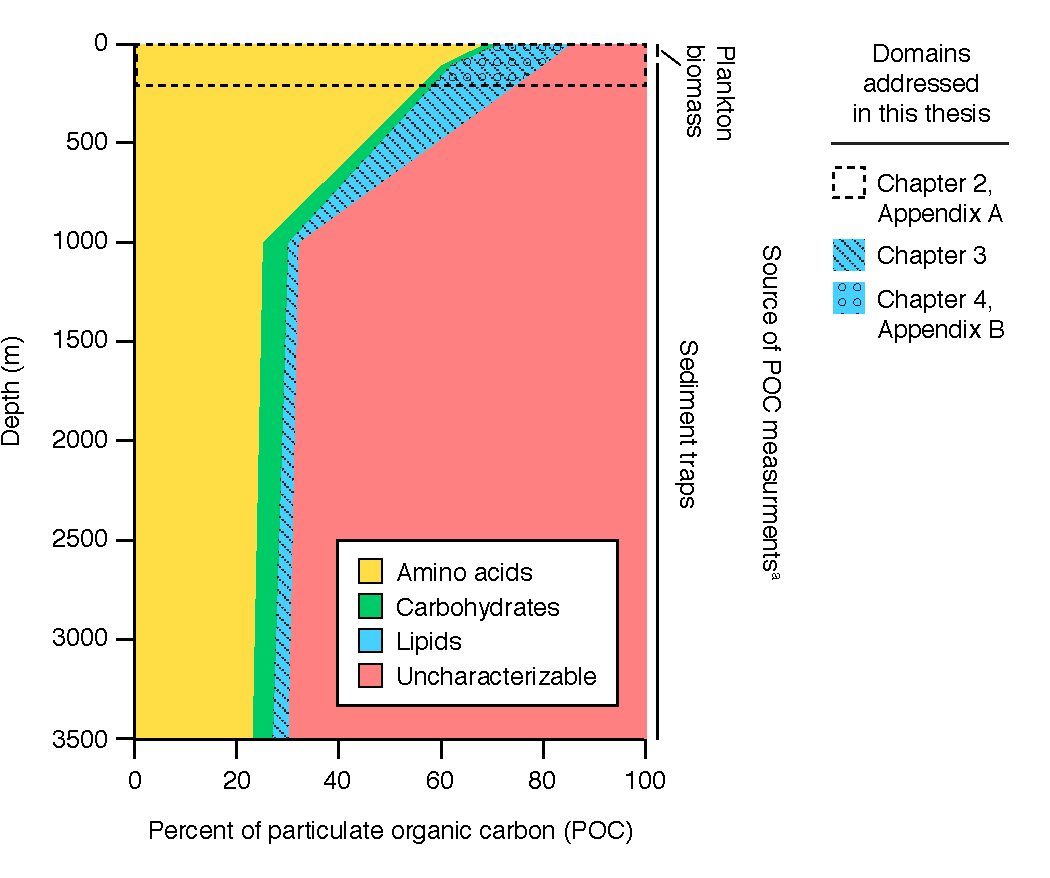
\includegraphics[width=0.75\textwidth]{Fig_1-1.pdf}
\captionsetup{font={footnotesize}}
\caption[Concept of the thesis in relation to the relative proportions of biochemicals in organic matter at different depths in the ocean.]{Percentage of particulate organic carbon in three of the four major classes of biochemicals, as determined in samples collected at various depths in the central equatorial Pacific by Wakeham et al. (1997). Depicted in red is the large fraction of organic matter that could not be characterized at the molecular level. Superimposed over the figure are the chemical and depth domains addressed by various chapters of the thesis. \textsuperscript{a} As reported by Wakeham et al. (1997). The sediment trap samples were collected at 105, 1000, and $\geq$ 3500 m.}
\label{fig:c1n1}
\end{figure}

\begin{figure}[!p]
\centering
\includegraphics[width=0.75\textwidth]{Fig_1-2.pdf}
\captionsetup{font={footnotesize}}
\caption[Schematic showing the major processes that ultimately remove sinking particle material in the mesopelagic ocean, as conceptualized in \autoref{chap2} of the thesis.]{Schematic showing the major processes that ultimately remove sinking particle material in the mesopelagic ocean, as conceptualized in \autoref{chap2} of the thesis (Collins et al., 2015). Also shown are the accompanying first-order rate constants ($k$; units of day$^{-1}$) through which we represent these attenuation processes in the model described in that chapter. Arrow a, in magenta: Respiration of particle material by particle-attached heterotrophic bacteria ($k_{R}$, which we calculate from direct measurements). We use a single rate constant ($k_{S,D,Z}$) in our model sensitivity analyses to account for the other processes (arrows b-e), which we did not directly observe. $k_{S,D,Z}$ represents the fraction of particle flux attenuation that cannot be attributed to direct respiration by particle-attached bacteria. Arrow b, in orange: Enzymatic solubilization or mechanical disaggregation of particle material by attached bacteria. This process transfers organic matter to the dissolved or suspended phases in the surrounding water column, where it can then be metabolized by free-living bacterial communities (arrows f and g). Arrows c-e, in green: Particle flux attenuation processes attributable to zooplankton, including (arrow c) mechanical disaggregation (e.g., ``sloppy feeding''), (arrow d) egestion or excretion, or (arrow e) direct respiration of material to carbon dioxide. Disaggregation and excretion can transfer particle material to the dissolved or suspended phases; egestion of smaller fecal pellets can also transfer material to the suspended organic matter pool. Our interpretation of the sensitivity analysis results was informed by additional direct observations of arrow g.\\\\\tiny{Reproduced with permission from:\\\\Collins, J. R., B. R. Edwards, K. Thamatrakoln, J. E. Ossolinski, G. R. DiTullio, K. D. Bidle, S. C. Doney, and B. A. S. Van Mooy. 2015. The multiple fates of sinking particles in the North Atlantic Ocean. \emph{Global Biogeochemical Cycles} \emph{29}:1471-1494; doi:10.1002/2014GB005037\\\\\copyright 2015 American Geophysical Union}}
\label{fig:c1n2}
\end{figure}

First, in \autoref{chap2}, I sought to determine the relative contribution to particle flux attenuation by respiration compared to the other major biological and mechanical processes that progressively remove sinking particles with depth (\autoref{fig:c1n2}). I first present measurements collected at six stations in North Atlantic basin of sinking particulate carbon fluxes, water column bacterial production and respiration rates, and specific respiration rates on sinking particle material. I then calculate substrate-specific respiration rates on sinking particles, bacterial growth efficiencies (BGE) both in the water column and on sinking particle material, and depth-integrated estimates of water column BP and respiration for the upper mesopelagic zone (50 to 150 m). Finally, I apply the measurements of particulate organic carbon (POC) fluxes and substrate-specific respiration in a series of sensitivity analyses of a simple, yet mechanistic model of particle flux attenuation. Observational data and the results of these sensitivity analyses are combined to (1) constrain the relative contribution to particle flux attenuation by particle-attached microbial respiration compared to other processes and (2) determine how differences in the average sinking speed of marine particles affect this partitioning.

In \autoref{chap3}, I present a new software package and computational strategy for discovering lipid, oxylipin, and oxidized lipid biomarkers in large volumes of high-resolution, accurate-mass HPLC-ESI-MS lipid data. I was inspired in developing the software by the need for new computational approaches to parse the increasingly complex dataset that are generated in metabolomics and lipidomics studies (Cajka and Fiehn, 2016; Prosser et al., 2014). Lipid and Oxylipin Biomarker Screening through Adduct Hierarchy Sequences, or LOBSTAHS, is centered around a novel screening methodology that exploits the unique tendency of lipids to form adduct ions in consistent, diagnostic patterns of abundance that remain relatively consistent across sample types. Using lipid data from cultures of a mutant strain of a marine diatom (\emph{Phaeodactylum tricornutum}) designed for studies of oxidative stress (van Creveld et al., 2015), LOBSTAHS is applied in \autoref{chap3} to resolve conflicting compound assignments, examine differential expression of compounds across experimental treatments, discover and identify potential oxidized intact polar lipid (ox-IPL) and oxylipin biomarkers, and identify potential isomers and isobars. In the experimental dataset, a stress response is induced in the \emph{P. tricornutum} by treating the cultures with hydrogen peroxide (H$_2$O$_2$), a reactive oxygen species (ROS) that can be generated both biologically (e.g., as a consequence of metabolic activity) and abiotically (e.g., via photochemical reactions). H$_2$O$_2$ represents a persistent source of stress in many marine ecosystems.

\begin{figure}[!th]
\centering
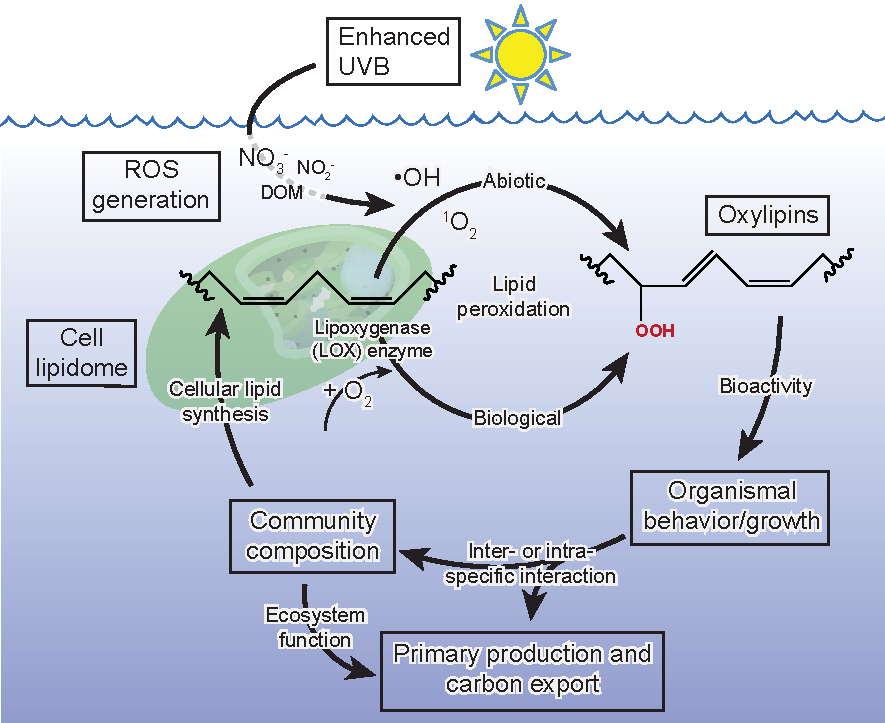
\includegraphics[width=1\textwidth]{Fig_1-3.pdf}
\captionsetup{font={footnotesize}}
\caption[Schematic illustrating the mechanisms through which oxidized lipids and oxylipins can be generated marine ecosystems, and the relationships between lipid peroxidation and several major biogeochemical and ecological processes.]{Schematic illustrating the mechanisms through which oxidized lipids and oxylipins can be generated marine ecosystems, and the relationships between lipid peroxidation and several major biogeochemical and ecological processes. In \autoref{chap4}, this conceptual framework is applied to the study of lipid photooxidation in surface waters of the West Antarctic Peninsula.
}
\label{fig:c1n3}
\end{figure}

In \autoref{chap4}, I explore the mechanisms and biogeochemical significance of lipid photooxidation in coastal surface waters of the West Antarctic Peninsula. The research in \autoref{chap4} was motivated by a paucity of information about the potentially complex relationships between ecosystem processes and the photochemical production of oxidized lipids and oxylipins induced by ultraviolet radiation (\autoref{fig:c1n3}). I combine results from experiments in a model liposome system with diverse environmental data --- including high-resolution, accurate-mass HPLC-ESI-MS analysis of lipid samples and in situ time-series measurements of ultraviolet irradiance --- to address several research objectives. By exposing liposomes to different light treatments under natural conditions, I sought to determine whether the photooxidation of intact polar diacylglycerols (IP-DAG; a broad class of membrane lipid) was dependent on molecular structure. Specifically, I hypothesized that a higher degree of unsaturation in the fatty acids of a particular IP-DAG would make it more amenable to photooxidation. As part of these experiments, I also investigated the effect of lipid photooxidation on natural communities of heterotrophic bacteria, and conversely, whether the presence of these bacteria would enhance apparent overall rates of lipid degradation. The diversity, quantities, and structures of various products of lipid photooxidation are queried by applying the data analysis methods described in \autoref{chap3} (Collins et al., 2016) to the HPLC-ESI-MS data from our liposome experiments. Using the same MS and data analysis methods, I also sought to characterize the lipidome of plankton from the WAP water column to determine what fraction of the particulate ($\geq$ 0.2 $\mu$m) lipid biomass would likely be amenable to degradation by photooxidation. Finally, I calculate broadband polychromatic apparent quantum yields (AQY) for photooxidation of IP-DAG under natural environmental conditions. These are applied to the water column lipid data and measurements of irradiance to estimate the significance of lipid photooxidation within the carbon cycle of the WAP ecosystem.

Finally, in \autoref{chap5}, I offer some new perspectives on the results and methods presented in the three main thesis chapters, and present some conclusions and directions for future research.

The thesis also contains several appendices: In \autoref{AppA}, I present a description and demonstration of the PHORCYS (PHOtosynthesis, Respiration, and Carbon-balance Yielding System), a new, incubation-based instrument that can be deployed in situ to determine rates of respiration and primary production in a wide range of marine and aquatic ecosystems. Development and testing of the PHORCYS was motivated by a surprising finding: Despite the attention that aerobic respiration has received relative to other processes that remineralize and degrade organic matter in the ocean, there are still far fewer total observations in the literature of respiration than primary production (\autoref{fig:c1n4}; le B. Williams and del Giorgio, 2005). Large discrepancies have also been observed between geochemical tracer and in vitro-based methods for measuring the net community productivity of marine ecosystems (le B. Williams et al., 2013). In \autoref{AppA}, respiration rate estimates from two versions of the PHORCYS are compared with estimates based a traditional method using Winkler titrations. A new method for estimating rates of error in metabolic rate measurements derived from dissolved oxygen time series is also presented. In \autoref{AppB}, I present some preliminary results from an experiment in which whole, unfiltered surface seawater samples from a site in the North Pacific Subtropical Gyre (NPSG) were exposed to different qualities of natural radiation during a series of shipboard incubations. The lipidomics pipeline described in \autoref{chap4} is applied to samples from the experiment to discover patterns and biomarkers of lipid photooxidation. The additional appendices (\autoref{AppC}, \autoref{AppD}, and \autoref{AppE}) contain supporting information, including supplementary figures and tables, for the main thesis chapters.

\begin{figure}[!th]
\centering
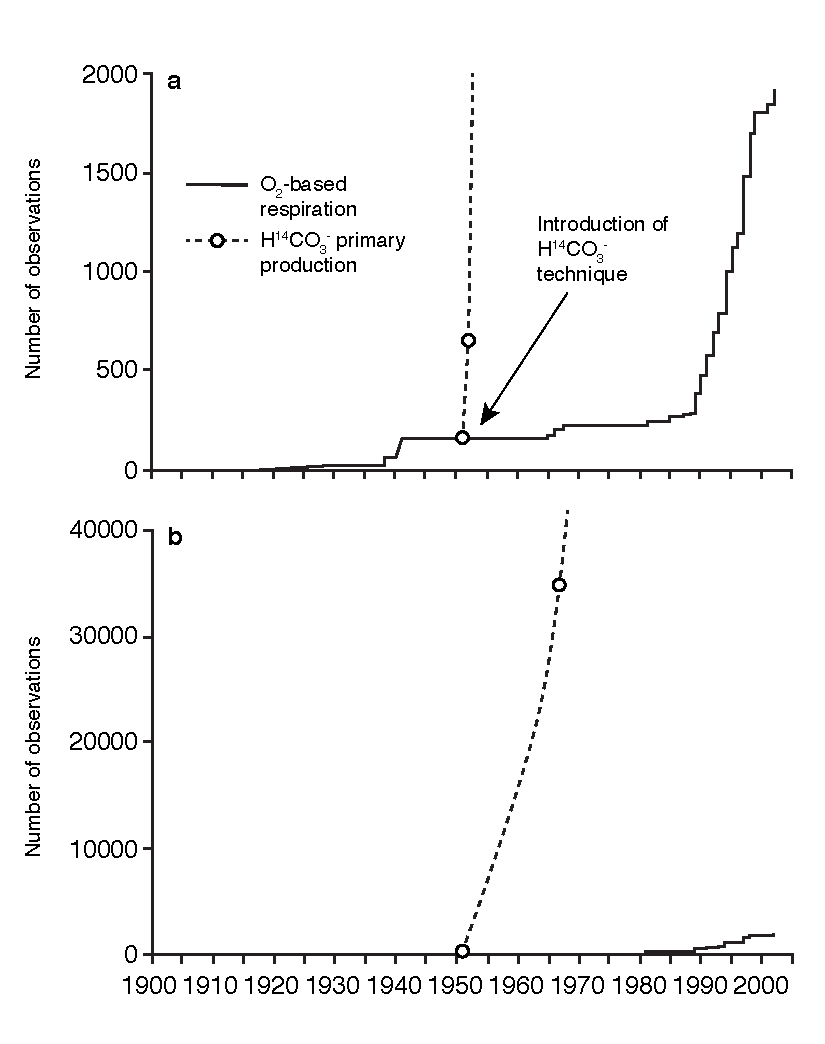
\includegraphics[width=.75\textwidth]{Fig_1-4.pdf}
\captionsetup{font={footnotesize}}
\caption[Cumulative estimate of the number of observations of aerobic respiration from measurements of dissolved oxygen and observations of primary production based on the H$^{14}$CO$_3^-$ method.]{Cumulative estimate of the number of observations of aerobic respiration from measurements of dissolved oxygen (solid line) and observations of primary production based on the H$^{14}$CO$_3^-$ method (dashed line). The figure is modified from Williams and del Giorgio (2005). Panel (a) shows the same data as panel (b), but with a 20-fold expansion of the \emph{y}-axis.}
\label{fig:c1n4}
\end{figure}

In preparing this thesis, I was keenly aware of a widely-held perception that geoscientists have been slow to adopt many of the core tenets of open science (McNutt et al., 2016). Accordingly, I have endeavored to make all data, software, and code required to reproduce the results in this thesis publicly available in open-source or non-proprietary formats; instructions can be found in designated sections at the end of each chapter, or in the corresponding supporting information. I sincerely apologize that some of my earlier computations (for \autoref{chap2}) were performed in MATLAB. MATLAB is a great product, but it costs a considerable amount of money for those who don't have access to a site license. With this caveat, I have hewed as closely as possible to the guidelines established by the \href{http://www.scientificpaperofthefuture.org/gpf/what-is-a-gpf}{Geoscience Papers of the Future Initiative} for provenance and data and software availability.
\clearpage
\begin{singlespace}
\section*{References}
\addtocounter{section}{1}
{\setlength{\parindent}{0pt}
Ar\'{i}stegui, J., C. M. Duarte, S. Agust\'{i}, M. Doval, X. A. \'{A}lvarez-Salgado,
and D. A. Hansell (2002), Dissolved organic carbon support of
respiration in the dark ocean, \emph{Science}, \emph{298}(5600),
1967-1967, doi:\href{http://dx.doi.org/10.1126/science.1076746}{10.1126/science.1076746}.

{\setlength{\parskip}{10pt}

Arrhenius, S. (1896), On the influence of carbonic acid in the air upon the temperature of the ground, \emph{London, Edinburgh and Dublin Philosophical Magazine and Journal of Science}, \emph{41}, 237-276.

Berner, R. A. (1981), A new geochemical classification of sedimentary
environments, \emph{Journal of Sedimentary Research}, \emph{51}(2),
359-365, doi:\href{http://dx.doi.org/10.1306/212f7c7f-2b24-11d7-8648000102c1865d}{10.1306/212f7c7f-2b24-11d7-8648000102c1865d}.

Broecker, W. S. (1983), The ocean, \emph{Scientific American}, \emph{249}, 146-161.

Cajka, T., and O. Fiehn (2016), Toward merging untargeted and targeted
methods in mass spectrometry-based metabolomics and lipidomics,
\emph{Analytical Chemistry}, \emph{88}(1), 524-545,
doi:\href{http://dx.doi.org/10.1021/acs.analchem.5b04491}{10.1021/acs.analchem.5b04491}.

Carlson, C. A., and H. W. Ducklow (1996), Growth of bacterioplankton and
consumption of dissolved organic carbon in the Sargasso Sea,
\emph{Aquatic Microbial Ecology}, \emph{10}(1), 69-85.

Chamberlin, T. C. (1898), The influence of great epochs of limestone formation upon the constitution of the atmosphere, \emph{Journal of Geology}, \emph{6}, 609-621.

Close, H. G., S. R. Shah, A. E. Ingalls, A. F. Diefendorf, E. L. Brodie,
R. L. Hansman, K. H. Freeman, L. I. Aluwihare, and A. Pearson (2013),
Export of submicron particulate organic matter to mesopelagic depth in
an oligotrophic gyre, \emph{Proceedings of the National Academy of Sciences of the United States of America}, \emph{110}(31),
12565-12570, doi:\href{http://dx.doi.org/10.1073/pnas.1217514110}{10.1073/pnas.121751411\\0}.

Collins, J. R., B. R. Edwards, K. Thamatrakoln, J. E. Ossolinski, G. R.
DiTullio, K. D. Bidle, S. C. Doney, and B. A. S. Van Mooy (2015), The
multiple fates of sinking particles in the North Atlantic Ocean,
\emph{Global Biogeochemical Cycles}, \emph{29}, 1471-1494,
doi:\href{http://dx.doi.org/10.1002/2014GB005037}{10.1002/2014GB005\\037}.

D. Krom, M., and R. A. Berner (1981), The diagenesis of phosphorus in a
nearshore marine sediment, \emph{Geochimica et Cosmochimica Acta},
\emph{45}(2), 207-216, doi:\href{http://dx.doi.org/10.1016/0016-7037(81)90164-2}{10.1016/0016-7037(81)90164-2}.

del Giorgio, P. A., and C. M. Duarte (2002), Respiration in the open
ocean, \emph{Nature}, \emph{420}(6914), 379-384.

del Giorgio, P. A., J. J. Cole, and A. Cimbleris (1997), Respiration
rates in bacteria exceed phytoplankton production in unproductive
aquatic systems, \emph{Nature}, \emph{385}(6612), 148-151.

Ducklow, H. W., and S. C. Doney (2013), What is the metabolic state of
the oligotrophic ocean? A debate, \emph{Annual Review of Marine Science}, \emph{5},
15.11--15.19, doi:\\\href{http://dx.doi.org/10.1146/annurev-marine-121211-172331}{10.1146/annurev-marine-121211-172331}.

Dugdale, R. C., and J. J. Goering (1967), Uptake of new and regenerated forms of nitrogen in primary productivity, \emph{Limnology \& Oceanography}, \emph{12}(2), 196-206.

Eppley, R. W., and B. J. Peterson (1979), Particulate organic matter flux and planktonic new production in the deep ocean, \emph{Nature}, \emph{282}(5740), 677-680.

Falkowski, P. G. (2014), Biogeochemistry of primary production in the
sea, in \emph{Treatise on Geochemistry (Second Edition)}, edited by K.
K. Turekian, pp. 163-187, Elsevier, Oxford,
doi:\href{http://dx.doi.org/10.1016/B978-0-08-095975-7.00805-6}{10.1016/B978-0-08-095975-7.00805-6}.

Giering, S. L. C., et al. (2014), Reconciliation of the carbon budget in
the ocean's twilight zone, \emph{Nature}, \emph{507}(7493), 480-483,
doi:\href{http://dx.doi.org/10.1038/nature13123}{10.1038/nature13123}.

Gorham, E. (1991), Biogeochemistry: its origins and development, \emph{Biogeochemistry}, \emph{13}(3), 199-239.

Grossart, H. P., A. Engel, C. Arnosti, C. L. De La Rocha, A. E. Murray,
and U. Passow (2007), Microbial dynamics in autotrophic and
heterotrophic seawater mesocosms. III. Organic matter fluxes,
\emph{Aquatic Microbial Ecology}, \emph{49}(2), 143-156,
doi:\href{http://dx.doi.org/10.3354/ame01140}{10.3354/ame01140}.

Hedges, J. I., J. A. Baldock, Y. Gelinas, C. Lee, M. Peterson, and S. G.
Wakeham (2001), Evidence for non-selective preservation of organic
matter in sinking marine particles, \emph{Nature}, \emph{409}(6822),
801-804.

Hunter, J. E., M. J. Frada, H. F. Fredricks, A. Vardi, and B. A. S. Van
Mooy (2015), Targeted and untargeted lipidomics of \emph{Emiliania huxleyi}
viral infection and life cycle phases highlights molecular biomarkers of
infection, susceptibility, and ploidy, \emph{Frontiers in Marine
Science}, \emph{2}, doi:\href{http://dx.doi.org/10.3389/fmars.2015.00081}{10.3389/fmars.2015.00081}.

Keil, R. G., D. B. Montlucon, F. G. Prahl, and J. I. Hedges (1994),
Sorptive preservation of labile organic matter in marine sediments,
\emph{Nature}, \emph{370}(6490), 549-552.

Kieber, D. J., J. McDaniel, and K. Mopper (1989), Photochemical source
of biological substrates in sea water: implications for carbon cycling,
\emph{Nature}, \emph{341}(6243), 637-639.

Killops, S. D., and V. J. Killops (2005), \emph{An Introduction to
Organic Geochemistry}, 2nd ed., 408 pp., Wiley-Blackwell, New York.

McNutt, M., K. Lehnert, B. Hanson, B. A. Nosek, A. M. Ellison, and J. L.
King (2016), Liberating field science samples and data, \emph{Science},
\emph{351}(6277), 1024-1026, doi:\href{http://dx.doi.org/10.1126/science.aad7048}{10.1126/science.a\\ad7048}.

Middelburg, J. J. (1989), A simple rate model for organic matter
decomposition in marine sediments, \emph{Geochimica et Cosmochimica Acta},
\emph{53}(7), 1577-1581, doi:\href{http://dx.doi.org/10.1016/0016-7037(89)90239-1}{10.1016/0016-7037(89)90239-1}.

Miller, W. L., and R. G. Zepp (1995), Photochemical production of
dissolved inorganic carbon from terrestrial organic matter: Significance
to the oceanic organic carbon cycle, \emph{Geophysical Research Letters},
\emph{22}(4), 417-420, doi:\href{http://dx.doi.org/10.1029/94GL03344}{10.1029/94GL03344}.

Mopper, K., and D. J. Kieber (2002), Photochemistry and the cycling of
carbon, sulfur, nitrogen and phosphorous, in \emph{Biogeochemistry of
Marine Dissolved Organic Matter}, edited by D. A. Hansell and C. A.
Carlson, pp. 455-489, Academic Press, New York.

Mopper, K., X. Zhou, R. J. Kieber, D. J. Kieber, R. J. Sikorski, and R.
D. Jones (1991), Photochemical degradation of dissolved organic carbon
and its impact on the oceanic carbon cycle, \emph{Nature},
\emph{353}(6339), 60-62.

Mottl, M. J., and H. Elderfield (2014), Volume editor's introduction, in \emph{Treatise on Geochemistry (Second Edition)}, edited by K. K. Turekian, pp. xxiii-xxv, Elsevier, Oxford, doi:\href{http://dx.doi.org/10.1016/B978-0-08-095975-7.09985-X}{10.1016/B978-0-08-095975-7.09985-X}.

Pearson, A. (2014), Lipidomics for geochemistry, in \emph{Treatise on
Geochemistry}, edited by H. D. Holland and K. K. Turekian, pp. 291-336,
Elsevier, Oxford.

Perrault, P. (1674), \emph{De l'origine des fontaines} (\emph{On the Origin of Springs}, translated by Hafner, 1966).

Petsch, S. T. (2014), Weathering of organic carbon, in \emph{Treatise on
Geochemistry (Second Edition)}, edited by K. K. Turekian, pp. 217-238,
Elsevier, Oxford, doi:\href{http://dx.doi.org/10.1016/B978-0-08-095975-7.01013-5}{10.1016/B978-0-08-095975-7.01013-5}.

Ploug, H., and H.-P. Grossart (1999), Bacterial production and
respiration in suspended aggregates --- a matter of the incubation
method, \emph{Aquatic Microbial Ecology}, \emph{20}, 21-29.

Prosser, G. A., G. Larrouy-Maumus, and L. P. de Carvalho (2014),
Metabolomic strategies for the identification of new enzyme functions
and metabolic pathways, \emph{EMBO Reports}, \emph{15}(6), 657-669,
doi:\href{http://dx.doi.org/10.15252/embr.201338283}{10.15252/embr.201338283}.

Rontani, J.-F., B. Charriere, A. Forest, S. Heussner, F. Vaultier, M.
Petit, N. Delsaut, L. Fortier, and R. Sempere (2012), Intense
photooxidative degradation of planktonic and bacterial lipids in sinking
particles collected with sediment traps across the Canadian Beaufort
Shelf (Arctic Ocean), \emph{Biogeosciences}, \emph{9}(11), 4787-4802,
doi:\href{http://dx.doi.org/10.5194/Bg-9-4787-2012}{10.5194/Bg-9-4787-2012}.

Rontani, J.-F., B. Charriere, M. Petit, F. Vaultier, H. J. Heipieper, H.
Link, G. Chaillou, and R. Sempere (2012), Degradation state of organic
matter in surface sediments from the Southern Beaufort Sea: a lipid
approach, \emph{Biogeosciences}, \emph{9}(9), 3513-3530,
doi:\href{http://dx.doi.org/10.5194/Bg-9-3513-2012}{10.5194/Bg-9-3513-2012}.

Stemmann, L., G. A. Jackson, and G. Gorsky (2004), A vertical model of
particle size distributions and fluxes in the midwater column that
includes biological and physical processes---Part II: application to a
three year survey in the NW Mediterranean Sea, \emph{Deep Sea Research
Part I: Oceanographic Research Papers}, \emph{51}(7), 885-908,
doi:\href{http://dx.doi.org/10.1016/j.dsr.2004.03.002}{10.1016/j.dsr.2004.03.002}.

Sturt, H. F., R. E. Summons, K. Smith, M. Elvert, and K. U. Hinrichs
(2004), Intact polar membrane lipids in prokaryotes and sediments
deciphered by high-performance liquid chromatography/electrospray
ionization multistage mass spectrometry - new biomarkers for
biogeochemistry and microbial ecology, \emph{Rapid Communications in Mass Spectrometry}, \emph{18}(6), 617-628, doi:\href{http://dx.doi.org/10.1002/rcm.1378}{10.1002/rcm.1378}.

Sundquist, E. T., and K. V. Ackerman (2014), The geologic history of the carbon cycle, in \emph{Treatise on Geochemistry (Second Edition)}, edited by K. K. Turekian, pp. 361-398, Elsevier, Oxford, doi:\href{http://dx.doi.org/10.1016/B978-0-08-095975-7.00809-3}{10.1016/B978-0-08-095975-7.00809-3}.

van Creveld, S. G., S. Rosenwasser, D. Schatz, I. Koren, and A. Vardi
(2015), Early perturbation in mitochondria redox homeostasis in response
to environmental stress predicts cell fate in diatoms, \emph{The ISME Journal},
\emph{9}(2), 385-395, doi:\href{http://dx.doi.org/10.1038/ismej.2014.136}{10.1038/ismej.2014.136}.

Van Mooy, B. A. S., G. Rocap, H. F. Fredricks, C. T. Evans, and A. H.
Devol (2006), Sulfolipids dramatically decrease phosphorus demand by
picocyanobacteria in oligotrophic marine environments, \emph{Proceedings of the National Academy of Sciences of the United States of America}, \emph{103}(23), 8607-8612, doi:\href{http://dx.doi.org/10.1073/pnas.0600540103}{10.1073/pnas.0600540103}.

Van Mooy, B. A. S., et al. (2009), Phytoplankton in the ocean use
non-phosphorus lipids in response to phosphorus scarcity, \emph{Nature},
\emph{458}(7234), 69-72.

Vardi, A., L. Haramaty, B. A. Van Mooy, H. F. Fredricks, S. A. Kimmance,
A. Larsen, and K. D. Bidle (2012), Host-virus dynamics and subcellular
controls of cell fate in a natural coccolithophore population,
\emph{Proceedings of the National Academy of Sciences of the United
States of America}, \emph{109}(47), 19327-19332,
doi:\href{http://dx.doi.org/10.1073/pnas.1208895109}{10.1073/pnas.1208895109}.

Vernadsky, V. I. (1924), \emph{La G\'{e}ochimie}, Alcan, Paris.

Volk, T., and M. I. Hoffert (1985), Ocean carbon pumps: Analysis of relative strengths and efficiencies in ocean-driven atmospheric CO2 changes, in \emph{The Carbon Cycle and Atmospheric CO2: Natural Variations Archean to Present}, edited by E. T. Sundquist and W. S. Broecker, pp. 99-110, AGU, Washington, DC, doi:\href{http://dx.doi.org/10.1029/GM032p0099}{10.1029/GM032p0099}.

Wakeham, S. G., J. I. Hedges, C. Lee, M. L. Peterson, and P. J. Hernes
(1997), Compositions and transport of lipid biomarkers through the water
column and surficial sediments of the equatorial Pacific Ocean,
\emph{Deep Sea Research Part II: Topical Studies in Oceanography}, \emph{44}(9-10), 2131-2162,
doi:\href{http://dx.doi.org/10.1016/s0967-0645(97)00035-0}{10.1016/s0967-0645(97)00035-0}.

Wakeham, S. G., C. Lee, J. I. Hedges, P. J. Hernes, and M. J. Peterson
(1997), Molecular indicators of diagenetic status in marine organic
matter, \emph{Geochimica et Cosmochimica Acta}, \emph{61}(24), 5363-5369,
doi:\href{http://dx.doi.org/10.1016/S0016-7037(97)00312-8}{10.1016/S0016-7037(97)00312-8}.

Williams, P. J. le B. (1998), The balance of plankton respiration and
photosynthesis in the open oceans, \emph{Nature}, \emph{394}(6688),
55-57.

Williams, P. J. le B., and P. del Giorgio (2005), Respiration in aquatic
ecosystems: history and background, in \emph{Respiration in Aquatic
Ecosystems}, edited by P. del Giorgio and P. J. le B. Williams, Oxford
University Press, New York.

Williams, P. J. le B., P. D. Quay, T. K. Westberry, and M. J. Behrenfeld
(2013), The oligotrophic ocean is autotrophic, \emph{Annual Review of Marine Science}, \emph{5}, 16.11-16.15, doi:\href{http://dx.doi.org/10.1146/annurev-marine-121211-172335}{10.1146/\\annurev-marine-121211-172335}.

Zafiriou, O. C., S. S. Andrews, and W. Wang (2003), Concordant estimates
of oceanic carbon monoxide source and sink processes in the Pacific
yield a balanced global ``blue-water'' CO budget, \emph{Global
Biogeochemical Cycles}, \emph{17}(1), 1015, doi:\href{http://dx.doi.org/10.1029/2001GB001638}{10.1029/2001GB001638}.}}
\end{singlespace}
%% This is an example first chapter.  You should put chapter/appendix that you
%% write into a separate file, and add a line \include{yourfilename} to
%% main.tex, where `yourfilename.tex' is the name of the chapter/appendix file.
%% You can process specific files by typing their names in at the 
%% \files=
%% prompt when you run the file main.tex through LaTeX.

\begingroup%
\makeatletter%
\cleardoublepage%
\let\newpage\relax%
\let\clearpage\relax%
\vspace*{\fill}%
\vspace*{\dimexpr-50\p@-\baselineskip}% Remove the initial
%% -default- 50pt gap (plus 1 line) 
\chapter{The Multiple Fates of Sinking Particles in the North Atlantic Ocean}
\label{chap2}
\let\thefootnote\relax\footnote{{\setlength{\parindent}{0pt}This chapter was originally published as:\\\\Collins, J. R., B. R. Edwards, K. Thamatrakoln, J. E. Ossolinski, G. R. DiTullio, K. D. Bidle, S. C. Doney, and B. A. S. Van Mooy. 2015. The multiple fates of sinking particles in the North Atlantic Ocean. \emph{Global Biogeochemical Cycles} \emph{29}:1471-1494; doi:\href{http://dx.doi.org/10.1002/2014GB005037}{10.1002/2014GB005037}\\\\\copyright 2015 American Geophysical Union}}
\vspace*{\fill}%
\endgroup%

\clearpage
\section{Abstract}
The direct respiration of sinking organic matter by attached bacteria is often invoked as the dominant sink for settling particles in the mesopelagic ocean. However, other processes, such as enzymatic solubilization\textsuperscript{1}\let\thefootnote\relax\footnote{{\setlength{\parindent}{0pt}\textsuperscript{1} i.e., via exoenzyme hydrolysis. The term ``enzymatic solubilization'' is used throughout the chapter.}} and mechanical disaggregation, also contribute to particle flux attenuation by transferring organic matter to the water column. Here we use observations from the North Atlantic Ocean, coupled to sensitivity analyses of a simple model, to assess the relative importance of particle-attached microbial respiration compared to the other processes that can degrade sinking particles. The observed carbon fluxes, bacterial production rates, and respiration by water column and particle-attached microbial communities each spanned more than an order of magnitude. Rates of substrate-specific respiration on sinking particle material ranged from 0.007 $\pm$ 0.003 to 0.173 $\pm$ 0.105 day\textsuperscript{-1}. A comparison of these substrate-specific respiration rates with model results suggested sinking particle material was transferred to the water column by various biological and mechanical processes nearly 3.5 times as fast as it was directly respired. This finding, coupled with strong metabolic demand imposed by measurements of water column respiration (729.3 $\pm$ 266.0 mg C m\textsuperscript{-2} d\textsuperscript{-1}, on average, over the 50 to 150 m depth interval), suggested a large fraction of the organic matter evolved from sinking particles ultimately met its fate through subsequent remineralization in the water column. At three sites, we also measured very low bacterial growth efficiencies and large discrepancies between depth-integrated mesopelagic respiration and carbon inputs.
\clearpage
\section{Introduction}
The efficiency of the ocean's biological pump, one of the two primary mechanisms by which carbon dioxide is chemically reduced and exported to depth, is defined by a fine balance between primary production in the marine surface layer and the destruction of this organic matter in and below the euphotic zone. The majority of this export occurs as a rain of sinking particles that are progressively remineralized by heterotrophic bacteria or zooplankton as they sink through the mesopelagic ocean (Buesseler and Boyd, 2009; Buesseler et al., 2007b; Steinberg et al., 2008b). Respiration by particle-associated heterotrophic communities has been invoked in several specific ecosystems as the primary sink for these particles, based on observations either in the field or in the laboratory (e.g., McDonnell et al., 2015; Ploug et al., 1999) or statistical relationships, for example, between the remineralization length scale and temperature (Marsay et al., 2015). However, modeling exercises, together with an increasing number of environmental studies, indicate that a substantial fraction of particles from the ocean's surface can be degraded during their downward transit by other processes that rival particle-attached microbial respiration in magnitude (Close et al., 2013; Giering et al., 2014; Ki\o{}rboe, 2001; Ki\o{}rboe and Jackson, 2001; Stemmann et al., 2004a, 2004b; Taylor and Karl, 1991).

Observational and experimental evidence both suggest that particle disaggregation and solubilization can transfer sinking organic matter to the suspended particulate (POM\textsubscript{susp}) or dissolved organic matter (DOM) pools, as an alternative to direct respiration (Alldredge, 2000; Grossart and Simon, 1998; Smith et al., 1992). The POM\textsubscript{susp} and DOM can then provide an immediate metabolic substrate for free-living bacteria in the water column (Ki\o{}rboe and Jackson, 2001). Alternatively, dissolved organic matter can remain within the 662 Pg pool of marine dissolved organic carbon (DOC), where it may be later respired or instead removed by some other process (Azam, 1998; Hansell et al., 2009). Zooplankton can serve both as a sink for particle material, via respiration or mechanical disaggregation, and as a source of particles below the mixed layer. At depth, zooplankton can egest fecal pellets following their daily vertical migration from the ocean's surface (Steinberg et al., 2008b); they may also ``repackage'' suspended particles at depth into sinking particles.

Establishing the relative contributions of these various particle degradation processes to total observed particle flux attenuation remains a principal challenge in investigations of the marine carbon cycle, particularly at global and basin scales (Burd et al., 2010; Sanders et al., 2014; Siegel et al., 2014). The inability to accurately, precisely, and reliably quantify the relative importance of these processes has been identified as a significant source of uncertainty in continuing efforts to ascertain the metabolic state of various ocean ecosystems (Buesseler and Boyd, 2009; Ducklow and Doney, 2013). Many of these studies have identified order-of-magnitude imbalances in the mesopelagic and upper bathypelagic between inputs of settling organic matter and metabolic sinks, often with large uncertainties attached to the latter (del Giorgio et al., 1997; Duarte et al., 2013; Geider, 1997; Williams and Robertson, 1991; Reinthaler et al., 2006; Steinberg et al., 2008b). Even in the few recent studies that have narrowed or closed this mass imbalance, authors have relied on literature surveys, models, or significant interpolation for many of the sink terms associated with bacterial respiration and particle flux attenuation (Aranguren-Gassis et al., 2012; Giering et al., 2014; Westberry et al., 2012).

\begin{figure}[!p]
\centering
\includegraphics[width=0.75\textwidth]{Fig_2-1.pdf}
\captionsetup{font={footnotesize}}
\caption[Schematic showing the major processes that ultimately remove sinking particle material in the mesopelagic ocean, as conceptualized in \autoref{chap2}.]{Schematic showing the major processes that ultimately remove sinking particle material in the mesopelagic ocean, as conceptualized in \autoref{chap2} of the thesis (Collins et al., 2015). Also shown are the accompanying first-order rate constants ($k$; units of day$^{-1}$) through which we represent these attenuation processes in the model described in that chapter. Arrow a, in magenta: Respiration of particle material by particle-attached heterotrophic bacteria ($k_{R}$, which we calculate from direct measurements). We use a single rate constant ($k_{S,D,Z}$) in our model sensitivity analyses to account for the other processes (arrows b-e), which we did not directly observe. $k_{S,D,Z}$ represents the fraction of particle flux attenuation that cannot be attributed to direct respiration by particle-attached bacteria. Arrow b, in orange: Enzymatic solubilization or mechanical disaggregation of particle material by attached bacteria. This process transfers organic matter to the dissolved or suspended (i.e., colloidal) phases in the surrounding water column, where it can then be metabolized by free-living bacterial communities (arrows f and g). Arrows c-e, in green: Particle flux attenuation processes attributable to zooplankton, including (arrow c) mechanical disaggregation (e.g., ``sloppy feeding''), (arrow d) egestion or excretion, or (arrow e) direct respiration of material to carbon dioxide. Disaggregation and excretion can transfer particle material to the dissolved or suspended (i.e., colloidal) phases; egestion of smaller fecal pellets can also transfer material to the suspended organic matter pool. Our interpretation of the sensitivity analysis results was informed by additional direct observations of arrow g.}
\label{fig:c2n1}
\end{figure}

Here we sought to determine the relative contribution to particle flux attenuation by respiration compared to the other major biological and mechanical processes that progressively remove sinking particles with depth (\autoref{fig:c2n1}). While we focus in this study on the ultimate mass-balance sinks for these particles, complex mechanisms act to both disaggregate and re-aggregate particles continuously as they sink through the water column (Burd, 2013; Jackson and Burd, 1998). In this study, we first present measurements collected at six stations in North Atlantic basin (\autoref{fig:c2n2}) of sinking particulate carbon fluxes, water column bacterial production and respiration rates, and specific respiration rates on sinking particle material. From these data, we calculate substrate-specific respiration rates on sinking particles, bacterial growth efficiencies (\emph{BGE}) both in the water column and on sinking particle material, and depth-integrated estimates of water column BP and respiration for the upper mesopelagic zone (50 to 150 m). We then use our measurements of particulate organic carbon (POC) fluxes and substrate-specific respiration in a series of sensitivity analyses of a simple, yet mechanistic model of particle flux attenuation. Model-observed deviations allow us to place a minimum constraint at each station on the average particle sinking velocity, \emph{W\textsubscript{avg}}. We then combine our observational data and the results of these sensitivity analyses to (1) constrain the relative contribution to particle flux attenuation by particle-attached microbial respiration compared to other processes and (2) determine how differences in \emph{W\textsubscript{avg}} affect this partitioning. Our objective in quantifying this partitioning was to inform how respiration and other particle flux attenuation processes should be prioritized and parameterized in new models of marine carbon export (e.g., Siegel et al., 2014).

\section{Methods and Model Description}

\subsection{Cruises and Study Locations}


Conductivity-temperature-depth (CTD) data and water samples were collected on two cruises aboard the R/V \emph{Knorr} in 2012: BLATZ II (KN207-1; \url{http://www.bco-dmo.org/deployment/58787}) and NA VICE (KN207-3; \url{http://www.bco-dmo.org/project/2136}). The cruise tracks (\autoref{fig:c2n2}) allowed us to capture data for a variety of biogeographical provinces (Longhurst, 2010) in the North Atlantic Ocean over the course of 4 months. Deployments of sediment traps and shipboard incubations for determination of respiration rates in water column and sinking particle samples were performed during both cruises at six, 3 to 5 day, quasi-Lagrangian process stations. In addition, the rate of bacterial production was measured at each process station and along both cruise tracks. Process station locations were chosen based on physical and biological properties determined from real-time sea surface height and ocean color remote sensing data. Station PS-3 was reoccupied after approximately one week as station PS-4.

\subsection{Sediment Trap Deployments}

Vertically sinking particulate carbon fluxes were measured at 50, 150, and 300 m using surface-tethered cylindrical sediment traps (0.0125 m\textsuperscript{2} cross-sectional area; materials and construction as described in McDonnell and Buesseler (2012)). A mooring consisting of four traps at each depth, a surface buoy, wave-action mitigation bungee cord, and several floats, was deployed at each process station and allowed to drift for 3-5 days. The quasi-Lagrangian behavior of the mooring during each deployment was confirmed by comparison of positional data obtained from an Argos satellite beacon mounted on the surface buoy with shipboard acoustic Doppler current profiler data from the R/V \emph{Knorr}, which trailed the mooring at a range of 1-2 miles.

Traps were prepared, deployed, and recovered as described in McDonnell and Buesseler (2012). Traps were then sampled for particulate carbon in accordance with McDonnell and Buesseler (2012), except that the screened brine suspension (350 $\mu$m pore size, to exclude macrozooplankton) was filtered onto a series of precombusted, 47 mm GF/F filters (0.7 $\mu$m nominal pore size). Field and analytical blanks were collected at each station. Filters were immediately frozen in liquid nitrogen and then stored at -80$^{\circ}$C.

\subsection{Determination of Particulate Carbon Fluxes}

Filters from three of the four traps at each depth were used for determination of total particulate and particulate inorganic carbon (TPC and PIC, respectively). After thawing, the filters (including blanks) were first dried at 70$^{\circ}$C in a drying oven; each filter was then weighed and cut in half with precombusted stainless steel scissors. Each half was then weighed separately. One half was reserved for PIC analysis and the other reserved for determination of TPC. For TPC, sets of filter halves were transferred to 12 mm by 20 cm precombusted quartz tubes containing copper oxide (100 mg) and elemental silver wires. The tubes were then attached to a vacuum line, evacuated, flame-sealed, and combusted at 850$^{\circ}$C for 10 h. The evolved carbon dioxide was then isolated through a series of cold traps and quantified manometrically. PIC was determined from the other set of filter halves by coulometric analysis of acidified samples using a Model CM5014 UIC Coulometric Analyzer with Carbonate Acidification Module, as described in Honjo et al. (1995). Particulate organic carbon (POC) was determined for each trap by difference of the blank-corrected TPC and PIC measurements. An instrument failure in the laboratory prevented us from analyzing particle flux samples from station PS-1.

\subsection{Bacterial Production}

Water column bacterial production (BP) rates were measured at each process station and along both cruise tracks using the \textsuperscript{3}H-leucine incorporation microcentrifuge method of Simon and Azam (1989), as modified by Kirchman (2001). Incubations were conducted following each CTD cast using water samples from six depths; the first and sixth samples were always from the immediate surface layer (3-5 m) and 150 m. In addition, at process stations QL-1 and QL-2 (both on the eastern cruise leg), we conducted incubations for BP using sinking particle material retrieved from large-diameter net traps (see \autoref{ssec:Respiration by Bacteria Attached to Sinking Particles} below). Triplicate 1 mL samples from each chosen depth or net trap were incubated with \textsuperscript{3}H-leucine (PerkinElmer, Inc., Waltham, MA; 146.5 Ci mmol\textsuperscript{-1}, diluted to achieve 20 nM final concentration) for 4-12 h. Limited incubator space available for radiotracer work on the two cruises required us to incubate all BP samples from a given station at the same temperature. We chose a temperature that was most representative of the temperatures at the depths from which the majority of samples were drawn; this was, in almost all cases, the temperature of the mixed layer. Incubation of deeper samples (e.g., from 150 m) at this temperature could in some cases have biased the observed rates. However, we suspect such a temperature bias would only have been consequential at stations PS-2, PS-3, and PS-4, which were characterized by a significant vertical temperature gradient; at the other stations, the vertical temperature gradient did not exceed 3$^{\circ}$C (\autoref{fig:c2n3}e).

\begin{SCfigure}[0.5][!bh]
\centering
\includegraphics[width=0.6\textwidth]{Fig_2-2.pdf}
\captionsetup{font={footnotesize}}
\caption[Cruise tracks and sampling locations referenced in \autoref{chap2}.]{(a) Cruise tracks (blue, KN207-1 and red, KN207-3) and locations in the North Atlantic basin of the quasi-Lagrangian stations at which we conducted 3-5 day deployments of surface-tethered sediment traps and made measurements of respiration and bacterial production on sinking particle material. Symbols representing the locations of the six stations correspond to the data plotted in \autoref{fig:c2n3} and \autoref{fig:c2n4}. (b) Map expansion, showing locations of stations PS-3 and PS-4 superimposed over 8 day average MODIS Aqua surface reflectance at 555 nm. This parameter is an indicator of PIC concentration.}
\label{fig:c2n2}
\end{SCfigure}

At the conclusion of the two cruises, samples were processed and analyzed in a laboratory ashore according to Kirchman (2001) using Ultima Gold Low-Level Tritium cocktail (PerkinElmer, Inc.). Decay per minute counts in killed control samples were subtracted from the mean of each set of triplicates and divided by the incubation time to obtain a blank-corrected leucine incorporation rate (\emph{leu\textsubscript{inc}}) in units of pmol leucine L\textsuperscript{-1} h\textsuperscript{-1}.

To convert our volumetric measurements of \emph{leu\textsubscript{inc}} to carbon-based estimates of bacterial production (BP), we applied the basic equation
\begin{equation} \label{eq:c2e1}
BP = {\nu _{C:leu}}le{u_{inc}}ID
\end{equation}
where $\nu _{C:leu}$ $\nu _{C:leu}$ is a theoretical or empirical carbon to leucine conversion factor and \emph{ID} is a scaling factor that accounts for isotope dilution, i.e., the degree to which the added \textsuperscript{3}H-leucine was diluted within the cell by endogenous leucine sources. We employed two strategies with regard to the values of the scaling factors. First, to obtain individual estimates of water column and particle-attached bacterial production (\emph{BP\textsubscript{wc}} and \emph{BP\textsubscript{pa}}, respectively) in units of mg C m\textsuperscript{-3} d\textsuperscript{-1}, we applied a constant $\nu _{C:leu}$ of 1.5 kg C (mol leucine)\textsuperscript{-1} (Kirchman, 2001; Simon and Azam, 1989) and made the conservative assumption that \emph{ID} \emph{=}  1, i.e., that bacteria in our incubations had satisfied their leucine demand using only the added radiolabeled substrate. These are the results we report in \autoref{table:c2n2} and use for the upper axes in \autoref{fig:c2n3} and \autoref{fig:acn2} in the supporting information.

However, empirical evidence indicates that $\nu _{C:leu}$ and \emph{ID} both can vary considerably in the environment across depth, space, and time. \emph{ID} is difficult to measure and can represent a significant source of uncertainty in calculations of bacterial production (Chin-Leo and Kirchman, 1988; Ducklow and Hill, 1985; Kirchman, 2001). While variation in $\nu _{C:leu}$ is often more amenable to prediction (e.g., according to \emph{BGE}) (Alonso-Saez et al., 2008), it too varies widely (Giering et al., 2014). Therefore, as a second strategy, we used a bootstrap Monte Carlo analysis to consider wide variation in both of these parameters in our estimates of depth-integrated bacterial production, \emph{BP\textsubscript{int}}, from 50 to 150 m.

To obtain our estimates of \emph{BP\textsubscript{int}}, we followed the method of Giering et al. (2014), using the observational uncertainties in our water column measurements of \emph{leu\textsubscript{inc}} (\emph{N}  = 6 per station, as above) to fit a series of 100,000 bootstrap power law distributions to the data at each station, in increments of 0.1 m. A power law distribution provided the best empirical fit to the data from a range of simple functions we considered (\autoref{fig:c2n3}c). We then numerically integrated the bootstrap samples in each simulated data set from 50 to 150 m, according to
\begin{equation} \label{eq:c2e2}
B{P_{int}} = \int\limits_{z = 50}^{150} {le{u_{inc}}{\nu _{C:leu}}IDdz}
\end{equation}
In each simulation, we allowed \emph{ID} to take any value from 1 to 2, assuming a uniform distribution between the two extremes. We allowed $\nu _{C:leu}$ to vary according to a set of empirical values assembled from the literature by Giering et al. (2014) for depths \textgreater{} 50 m, which we assumed were normally distributed (\emph{N} = 21; mean $\pm$ standard deviation, 0.44 $\pm$ 0.27 kg C (mol leucine)\textsuperscript{-1}). We then used the mean and standard deviation of these repeated integrations to estimate a central value and uncertainty for \emph{BP\textsubscript{int}} at each station. This method allowed us to obtain estimates (\autoref{table:c2n3}) that reflected both observational uncertainties and possible variation in the two scaling factors.

\subsection{Photosynthetic Pigments}
\label{sec:Photosynthetic Pigments}

To evaluate the taxonomic composition of the phytoplankton community at each station, analysis of photosynthetic pigments was performed by high-performance liquid chromatography (HPLC). At each process station, water samples were collected from multiple depths via shipboard CTD and filtered onto precombusted 0.7 $\mu$m glass fiber filters. HPLC analysis was conducted in the laboratory according to DiTullio and Geesey (2003).

\subsubsection{Remote Sensing Data Analysis}

To generate the image in \autoref{fig:c2n1}b, we used 8-day average, level 3 MODIS AQUA satellite data of surface reflectance at 555 nm. A 4 km resolution data file (A201217720\\12184.L3m\_8D\_RRS\_Rrs\_555\_4km.hdf) was retrieved using the NASA GSFC\\OceanColor Level 3 Browser at \url{http://oceancolor.gsfc.nasa.gov/cgi/l3}. The false-color image was generated in ArcGIS 10.1 after geographical indexing.

\subsection{Respiration Measurements}

\subsubsection{Water Column Respiration}

Estimates of aerobic respiration by the water column microbial community (\emph{WCR}) were calculated by linear regression of measurements of dissolved oxygen concentration in a series of 300 mL shipboard bottle incubations. We made profiles of water column respiration at stations PS-2, PS-3, and PS-4; we made only one water column respiration measurement, in the euphotic zone, at each of the three other stations (QL-1, QL-2, and PS-1). Determination of dissolved oxygen was made at 3 to 9 h intervals in at least five replicates using optode spot minisensors (PreSens PSt3; Precision Sensing GmbH, Regensburg, Germany) that were glued to the inside surfaces of the bottles using food quality silicone cement (Warkentin et al., 2007). The use of these optode spots eliminated the need for drawing of aliquots from the sample bottles. Incubations were conducted in the dark at in situ temperature as described in Edwards et al. (2011). We validated the rates from these incubations using a series of Winkler titrations; methods are described in the supporting information. We used the standard error of the slope parameter from these regressions as the uncertainty in our estimates of \emph{WCR}. Depth-integrated water column respiration (\emph{WCR}\textsubscript{int}) was calculated from water column observations at stations PS-2, PS-3, and PS-4 (\emph{N} = 9, 6, and 7, respectively) using the same 100,000 simulation bootstrap method as for \emph{BP\textsubscript{int}}.

\subsubsection{Respiration by Bacteria Attached to Sinking Particles}
\label{ssec:Respiration by Bacteria Attached to Sinking Particles}

For determination of respiration by bacteria attached to sinking particles, particulate material was collected from the appropriate depth using a series of surface-tethered, large-diameter net traps with a detachable 0.2 $\mu$m mesh cod end (Peterson et al., 2005). These traps were allowed to drift from a surface mooring for approximately 24 h in the same eddy feature as the corresponding cylindrical sediment traps. The exact deployment time was controlled by use of a remote acoustic release, which allowed us to close the traps prior to recovery.
Upon recovery, the particle material in the cod end was homogenized by gentle shaking, then quantitatively split into fractions using an eight-way rotating electric splitter (Lamborg et al., 2008); aliquots were taken from one or more of these fractions, screened to 350 $\mu$m to exclude larger mesozooplankton, and dispensed quantitatively into replicate biochemical oxygen demand (BOD) bottles for incubation. The 350 $\mu$m screen was inspected to ensure it had not retained any particle material. Incubation bottles were then made up to volume with seawater retrieved by CTD cast from the same depth as the trap, and oxygen concentrations were monitored over time using optode sensor spots, as described above. An additional quantitative split was immediately collected by vacuum onto a precombusted 0.7 $\mu$m GF/F filter for determination of POC. POC was determined for these samples from the preserved filter by elemental analyzer (Carlo Erba Model 1108) after acid-fuming to remove the inorganic carbon fraction.

A substrate-specific respiration rate (\emph{k\textsubscript{R}}\textsubscript{;} units of mol C\textsubscript{respired}:mol POC d\textsuperscript{-1}) was determined from these measurements according to an adaptation of McDonnell (2011):
\begin{equation} \label{eq:c2e3}
{k_R} = \frac{{({r_{pa}} - {r_{col}}){V_{inc}}{\nu _{{\text{C:}}{{\text{O}}_{\text{2}}}}}}}{{PO{C_{trap}}}}
\end{equation}
where \emph{r\textsubscript{pa}} and \emph{r\textsubscript{col}} are volumetric respiration rates from the particle-attached and water column samples, respectively, calculated by simple linear regression from replicate shipboard incubations; \emph{V\textsubscript{inc}} is the incubation volume (300 mL); \emph{POC\textsubscript{trap}} is the quantity of POC used in the incubation; and $\nu _{{\text{C:}}{{\text{O}}_{\text{2}}}}$ is a molar respiratory quotient for the remineralization of organic matter at depth (we applied a value of 117/170) (Anderson and Sarmiento, 1994).

\subsubsection{Use of Winkler Titrations to Validate Respiration Rate Calculations}

To validate the water-column respiration rates we derived from our shipboard incubations, we used a simple method based on a series Winkler titrations. Winkler titration remains the standard analytical method for determination of dissolved oxygen in water (EPA Method 360.2 as modified for shipboard determination in seawater; U S EPA, 1983). For the comparison, we chose the depth in each respiration profile (\autoref{fig:c2n3}) that corresponded to the middle of the mixed layer (\autoref{table:c2n3}). We determined the respiration rate at this depth using triplicate samples sacrificed at two timepoints. A \emph{t} = 0 dissolved oxygen concentration was determined immediately in samples collected from the same CTD cast used for the respiration profile. A final concentration was determined using 300 mL samples that had been incubated alongside the optode sensor spot bottles. The respiration rate was determined by simple difference of the mean concentrations at the two timepoints.

\subsection{Bacterial Growth Efficiency}

Bacterial growth efficiency (\emph{BGE}) is a fundamental constraint on both bacterial growth and on microbial food web pathways that consume secondary production. It can be defined generally as the balance between bacterial production and bacterial respiration (BR) or
\begin{equation} \label{eq:c2e4}
BGE = \frac{{BP}}{{BP + BR}}
\end{equation}
We used our observations of \emph{BP\textsubscript{wc}} and \emph{WCR} to calculate the water column bacterial growth efficiency (\emph{BGE\textsubscript{wc}}) for depths \textgreater{} 50 m at stations PS-2, PS-3, and PS-4. We assumed in these calculations that, at these depths, our measurements of \emph{WCR = BR}; i.e., that no other microbiota (algae, protists, nanozooplankton, etc.) contributed to the oxygen consumption we observed in our incubations. We discuss the implications of this assumption for our results in \autoref{sssec:Enigmatically Low Efficiencies of Bacterial Growth}. We also calculated the growth efficiency on sinking particle material (\emph{BGE\textsubscript{pa}}) at stations QL-1 and QL-2, where we had observations of both particle-attached \emph{BP} and \emph{BR}.

\subsection{Sensitivity Analyses of a Simple Yet Mechanistic Flux Attenuation Model}

To complement our observations, we used sensitivity analyses of a simple model to diagnose the relative contributions to particle flux attenuation by direct respiration compared to other degradation processes. We also used these sensitivity analyses to place a minimum constraint on \emph{W\textsubscript{avg}} at each station. Models of particle flux attenuation range from the purely empirical, including the classic power law Martin curve, in which the exponent \emph{b} does not represent any particular thermodynamic process but can be used for comparison across ecosystems (Buesseler et al., 2007b; Martin et al., 1987), to models that attempt to account explicitly for the many complex mechanisms that form, destroy, and alter sinking particles (Anderson and Tang, 2010; Stemmann et al., 2004a).

\subsubsection{Model Specification}

Because our objective was to estimate generally the contribution to POC flux attenuation by particle-attached bacterial respiration compared to other possible processes, we chose to modify a simple, mechanistic, and frequently invoked exponential model of sinking particle flux attenuation that uses as primary inputs (1) sediment trap derived-particle fluxes and (2) rates of specific respiration on sinking particles (\emph{k\textsubscript{R}}; day\textsuperscript{-1}) (Boyd and Trull, 2007; Buesseler and Boyd, 2009; Lutz et al., 2002; McDonnell et al., 2015; Sarmiento and Gruber, 2006; Volk and Hoffert, 1985). In the model, the POC flux at a given depth \emph{z} (\emph{F\textsubscript{z}}, in mg C m\textsuperscript{-2} d\textsuperscript{-1}) is proportional to the flux observed at an overlying depth (\emph{F}\textsubscript{0}), which is attenuated according to first-order kinetics over a characteristic remineralization length scale (\emph{L\textsubscript{remin}}):
\begin{equation} \label{eq:c2e5}
{F_z} = {F_0}{e^{ - (z - {z_0})/{L_{remin}}}}
\end{equation}
A full derivation of \autoref{eq:c2e5} can be found in Sarmiento and Gruber (2006). We defined the length scale \emph{L\textsubscript{remin}} as the quotient of \emph{W\textsubscript{avg}} and the sum of two first-order rate constants that represent mechanistically, according to first-order kinetics, the processes (\autoref{fig:c2n1}) through which we assumed sinking POC could be oxidized or lost to the surrounding water column:
\begin{equation} \label{eq:c2e6}
{L_{remin}} = \frac{{{W_{avg}}}}{{{k_R} + {k_{S,D,Z}}}}
\end{equation}
\emph{k\textsubscript{R}} (day\textsuperscript{-1}) is the rate of oxidation of sinking POC by particle-attached bacteria, which we calculate from observations. \emph{k\textsubscript{S}}\textsubscript{,\emph{D},\emph{Z}} is a parameter of unknown magnitude that we use to estimate the rate of degradation of sinking POC by other processes; we diagnose the value of \emph{k\textsubscript{S}}\textsubscript{,\emph{D},\emph{Z}} using our sensitivity analyses to make comparisons with \emph{k\textsubscript{R}}.

In our conceptualization (\autoref{fig:c2n1}), the particle flux attenuation processes captured in \emph{k\textsubscript{S}}\textsubscript{,\emph{D},\emph{Z}} include (1) enzymatic solubilization (Azam and Malfatti, 2007) and (2) mechanical disaggregation, which transfer of sinking POC to the water column as dissolved organic carbon (DOC) or suspended POC (POC\textsubscript{susp}), and (3) various activities of zooplankton (discussed below). Solubilization occurs primarily via the activity of ectohydrolytic enzymes associated with bacterial cells, but can also be abiotic in origin (Taylor and Karl, 1991). Because ectoenzymes have high specificities for the different chemical components of sinking particle material, their relative contribution to disaggregation and dissolution will depend on how well the respective enzyme pool matches particle composition (Azam and Malfatti, 2007). Zooplankton can attenuate fluxes of sinking POC via mechanical disaggregation (e.g., ``sloppy feeding'' or ``zooplankton mining''), egestion or excretion or direct respiration. Shear stresses in the turbulent mixed layer are often strong enough to induce abiotic disaggregation of sinking particles, but evidence suggests abiotic shear does not play a major role in disaggregation in the ``quiescent'' mesopelagic ocean (Alldredge et al., 1990; Stemmann et al., 2004a). Although we do not consider mid-water shear in our conceptualization of particle flux attenuation, its effect would be captured in \emph{k\textsubscript{S}}\textsubscript{,\emph{D},\emph{Z}}.

Our definition of \emph{L\textsubscript{remin}} thus differs from previous parameterizations (e.g., McDonnell et al., 2015) by accounting in \emph{k\textsubscript{S}}\textsubscript{,\emph{D},\emph{Z}} for the losses of sinking particulate carbon to processes distinct from particle-attached bacterial respiration. Our parameterization does not allow us to further partition flux attenuation among these other processes (as in, e.g., Stemmann et al. (2004a)); however, our primary objective was only to estimate their collective strength compared to respiration by particle-attached bacteria. In addition, because we limited \autoref{eq:c2e5} and \autoref{eq:c2e6} to include a relatively small number of terms, we were required to diagnose or assume the values of only two unmeasured parameters, \emph{k\textsubscript{S}}\textsubscript{,\emph{D},\emph{Z}} and \emph{W\textsubscript{avg}}.

In applying \autoref{eq:c2e5} to sinking POC fluxes measured with surface-tethered sediment traps, we made several assumptions about the various biases inherent in the collection method. Horizontal shear can reduce the quantity of certain fractions of organic matter captured in moored traps relative to neutrally buoyant sediment traps or other collection methods (Stanley et al., 2004). Although there is evidence that the horizontal flow field can vary considerably across the depth range over which we made our measurements (Buesseler et al., 2007a), we assumed that any horizontal flow acted equally on the traps deployed at the three different depths, thus introducing a uniform bias for a given study site. We also assumed that the increase in the volume of ocean integrated by the traps at each successive depth (i.e., the ``statistical funnel'') (e.g., Siegel et al., 2008) was not so significant as to invalidate the use of measurements from different depths in the same model.

\subsubsection{Model Sensitivity Analyses and Bootstrap Monte Carlo Simulation}

We performed sensitivity analyses of the model over two depth intervals at five of our six stations (50-150 m and 150--300 m at QL-1, QL-2, PS-2, PS-3, and PS-4, yielding 10 observations of particle flux attenuation). Since we were able to fix the value of \emph{k\textsubscript{R}} at each station based on our observations, we used the sensitivity analyses to compute \emph{L\textsubscript{remin}} over a range of possible values for and \emph{k\textsubscript{S}}\textsubscript{,\emph{D},\emph{Z}}. We considered a range of values for \emph{W\textsubscript{avg}} (from 1 to 200 m d\textsuperscript{-1}, in 0.1 m d\textsuperscript{-1} increments) that encompassed those in the published literature for the temperate North Atlantic Ocean at depths \textless{} 1000 m; the results of our literature review are assembled in \autoref{table:acn1}. For \emph{k\textsubscript{S}}\textsubscript{,\emph{D},\emph{Z}}, we considered 1000 logarithmically distributed values from 10\textsuperscript{-5} d\textsuperscript{-1} (implying effectively no flux attenuation due to processes other than particle-attached bacterial respiration) to 1 day\textsuperscript{-1}, spanning several orders of magnitude and broadly encompassing our observed values of \emph{k\textsubscript{R}}. Because \emph{k\textsubscript{S}}\textsubscript{,\emph{D},\emph{Z}} was a parameter we created here to achieve our study objective, we found no truly equivalent values for it in the literature. At each station and depth interval, we then used the observational uncertainties in the inputs \emph{k\textsubscript{R}} and \emph{F}\textsubscript{0} to generate from \autoref{eq:c2e5} and \autoref{eq:c2e6} a simulated bootstrap data set of predictions of \emph{F\textsubscript{z}} (\emph{N} = 100,000) for each different pair of values of \emph{k\textsubscript{S}}\textsubscript{,\emph{D},\emph{Z}} and \emph{W\textsubscript{avg}}. We took the mean and standard deviation of each set of predictions to estimate the model flux (\emph{F\textsubscript{z}\textsubscript{,mod}}) and accompanying uncertainty ($\sigma_{mod}$) for each combination of \emph{k\textsubscript{S}}\textsubscript{,\emph{D},\emph{Z}} and \emph{W\textsubscript{avg}}.
ZXa
We then compared each model prediction (\emph{N} = $2\times10^6$ possible combinations per depth interval) to the observed flux at that station and depth (\emph{F\textsubscript{z}\textsubscript{,obs}}) using a simple measure of model-observed deviation (${F_{z,mod}} - {F_{z,obs}}$). Variation in this parameter at each station allowed us to diagnose the model's sensitivity to changes in \emph{k\textsubscript{S}}\textsubscript{,\emph{D},\emph{Z}} and \emph{W\textsubscript{avg}}. To determine whether the model-observed deviation was statistically significant, we tested the null hypothesis
\begin{equation} \label{eq:c2e7}
{H_0}:{F_{z,mod}} - {F_{z,obs}} = 0
\end{equation} 
at the $1\sigma$ confidence level. We rejected \emph{H}\textsubscript{0} where the absolute value of the model-observed deviation was greater than or equal to the root sum of the squared uncertainties or
\begin{equation} \label{eq:c2e8}
\left| {{F_{z,mod}} - {F_{z,obs}}} \right| \geq \sqrt {\sigma _{mod}^2 + \sigma _{obs}^2}
\end{equation} 
We used this test to assess a $1\sigma$ confidence region on the sensitivity analysis results at each station. We then excluded from further consideration those values of \emph{W\textsubscript{avg}} and \emph{k\textsubscript{S}}\textsubscript{,\emph{D},\emph{Z}} for which the model-observed deviation lay outside this region.

\section{Results and Discussion of Field Observations}

\subsection{POC and PIC Export}

Sinking particulate carbon fluxes captured with sediment traps varied geographically according to biogeochemical province and the composition of the phytoplankton community responsible for the majority of carbon fixation at each station (\autoref{fig:c2n3} and \autoref{table:c2n2}). POC fluxes at 50 m ranged from 47.9 $\pm$ 16.5 to 249 $\pm$ 16.3 mg C m\textsuperscript{-2} d\textsuperscript{-1}, while fluxes at 150 m ranged from 25.2 $\pm$ 2.0 to 208 $\pm$ 16.5 mg C m\textsuperscript{-2} d\textsuperscript{-1}. We observed the greatest variation in sinking carbon flux at 300 m; POC fluxes at that depth varied by a factor of 14, ranging from 9.6 $\pm$ 0.9 to 14.7 $\pm$ 4.6 mg C m\textsuperscript{-2} d\textsuperscript{-1} in oligotrophic waters (at station QL-2 in the Sargasso Sea and at station PS-2, respectively) to 131 $\pm$ 18.5 and 101 $\pm$ 12.3 mg C m\textsuperscript{-2} d\textsuperscript{-1} at the early and late stages of a summer coccolithophore bloom in subpolar waters (stations PS-3 and PS-4, respectively). By comparing the 50 m POC fluxes at stations PS-3 and PS-4 (249 $\pm$ 16.3 and 179 $\pm$ 33.7 mg C m\textsuperscript{-2} d\textsuperscript{-1}, respectively) with satellite-derived estimates of the duration (25 days) and total biomass fixed (24,000 t or 18.0 g m\textsuperscript{-2}) during a similar and simultaneous \emph{Emiliania huxleyi}-dominated bloom in the same region of the North Atlantic (Lehahn et al., 2014), we estimate that between 25 and 35\% of carbon fixed during the event could have been exported from the euphotic zone in the particulate phase. (The mean \emph{Z\textsubscript{eu}} for all stations in our study was 41 m; \autoref{table:acn2}.)

The ``rain ratio'' of POC to PIC, a measure of bulk flux composition, varied geographically as much as flux quantity. Occupying station PS-3 at the height of the coccolithophore bloom, we measured rain ratios of 2.3, 2.5, and 1.8 mol POC:mol PIC at 50, 150, and 300 m, respectively (\autoref{table:c2n1}). The relative contribution of PIC to total particulate carbon export decreased only slightly when the subpolar bloom site was reoccupied as station PS-4 the following week (\autoref{table:c2n2}). These low rain ratios were driven by the large PIC fluxes at the two stations (at 50 m, 109 $\pm$ 16.3 and, 1 week later, 42 $\pm$ 6.1 mg C m\textsuperscript{-2} d\textsuperscript{-1}). The rain ratios we documented at these two stations are among the lowest recorded for the North Atlantic and were consistent with patterns of export measured in quasi-Lagrangian mode during previous coccolithophore blooms (Foster and Shimmield, 2002; Schmidt et al., 2013). By comparison, the higher rain ratios we observed at the two stations on the western edge of the basin (16.6 and 13.4 for QL-1 and QL-2, respectively, at 50 m) were consistent with export from a diatom bloom observed at an earlier time of year in the eastern North Atlantic (Martin et al., 2011).

The dominant role of coccolithophores in driving primary production and export at the site of stations PS-3 and PS-4 was evident in both Moderate Resolution Imaging Spectroradiometer (MODIS) Aqua remote sensing imagery for the region (\autoref{fig:c2n2}b) and photosynthetic pigment data (\autoref{table:c2n2}). Surface reflectance at 555 nm, an indicator of biological calcium carbonate standing stock (Moore et al., 2012), remained elevated at the site throughout the time it was occupied (\autoref{fig:c2n2}b; remote sensing data analysis methods are described in the supporting information). HPLC pigment analysis of particulate samples also confirmed the dominance of coccolithophores at these stations: Of the four process stations on the eastern cruise track, PS-3 and PS-4 yielded samples with the highest ratios of $19'$-hexanoyloxyfucoxanthin ($19'$-hex) to fucoxanthin. This ratio can be used as a rough proxy for the abundance of coccolithophores relative to diatoms (\autoref{table:c2n2}) (Wright and Jeffrey, 1987).

Intense activity by coccolithoviruses is one possible means by which dead coccolithophore cell material at stations PS-3 and PS-4 was transformed into a PIC-dominated export flux. The active infection of \emph{Emiliania huxleyi} cells by these viruses (EhV) was shown to influence the development and senescence of a coccolithophore bloom within a nearby anticyclonic eddy observed during the same study (Lehahn et al., 2014). EhV infection at stations PS-3 and PS-4 was confirmed using flow cytometry, quantitative PCR, and diagnostic lipid biomarkers (K. D. Bidle, et al., unpublished data, 2015). EhVs have been shown to facilitate formation of transparent exopolymer particles (TEP) in the surface layer during bloom decline (Vardi et al., 2012); this TEP could have stimulated increased particulate carbon export at the stations via an aggregation mechanism similar to that described in Passow et al. (1994).

\subsection{Bacterial Production}
\label{ssec:Bacterial Production}

As with the quantity and composition of the particulate carbon flux, rates of water column bacterial production reflected both vertical (\autoref{fig:c2n3}) and latitudinal (\autoref{fig:acn2}) variations in biogeochemistry. Rates of leucine incorporation (\emph{leu\textsubscript{inc}}) above 25 pmol leu L\textsuperscript{-1} h\textsuperscript{-1} (equivalent to 0.94 mg C m\textsuperscript{-3} d\textsuperscript{-1}, assuming $\nu _{C:leu}$ = 1.5 kg C (mol leucine)\textsuperscript{-1} and \emph{ID} = 1) were generally confined to the surface mixed layer (upper 40 m of the water column) on both sides of the basin (\autoref{fig:c2n3} and \autoref{fig:acn2}); only on the immediate continental shelf east of New England (to far right in \autoref{fig:acn2}) was there evidence of significant bacterial production at greater depths. We obtained robust rates from the \textsuperscript{3}H-leucine microcentrifuge method at all but the deepest depths. Our killed control samples accounted for 12.5\%, on average, of the values obtained from the accompanying incubations; as expected, however, the signal-to-noise ratio was lower for deeper samples in which very low rates of leucine incorporation were measured (\autoref{fig:acn1}).

\begin{figure}[!p]
\centering
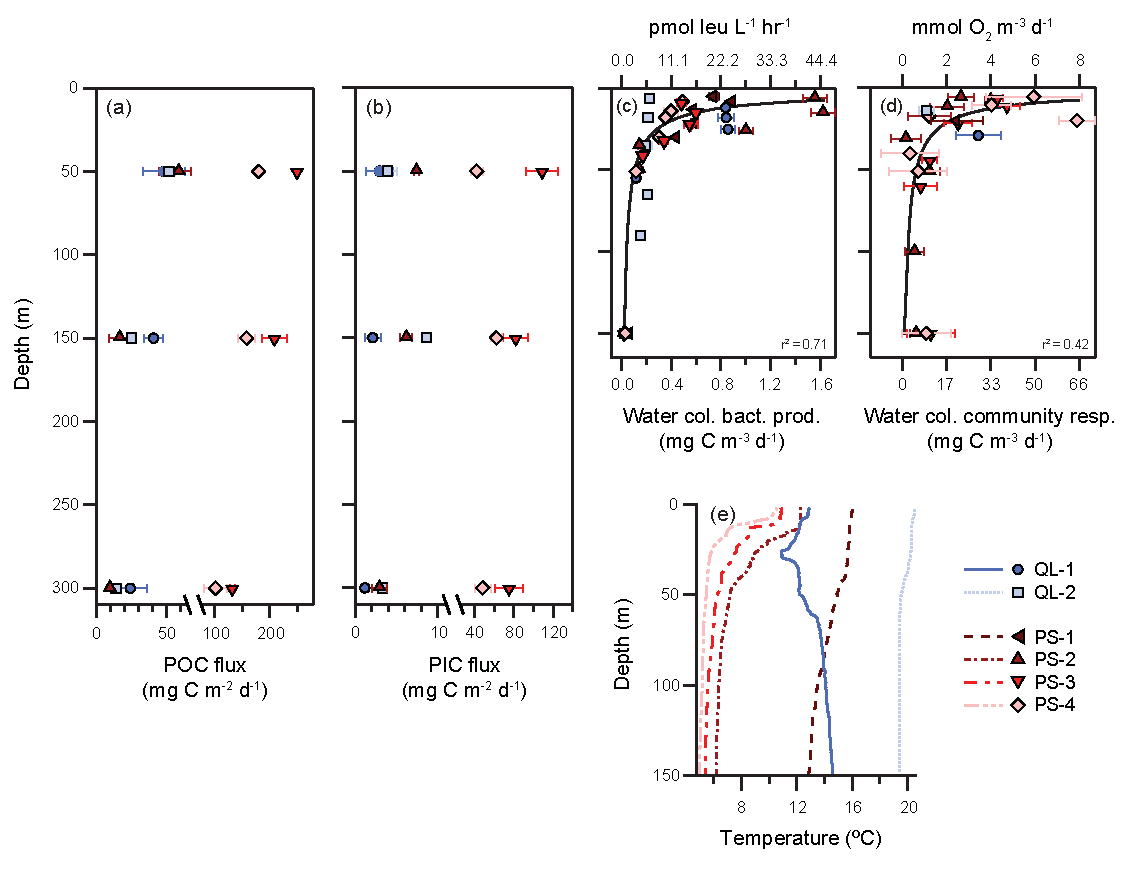
\includegraphics[width=1\textwidth]{Fig_2-3.pdf}
\captionsetup{font={footnotesize}}
\caption[Vertical profiles of sinking carbon fluxes and indicators of community metabolic activity at the six process stations described in the text.]{Vertical profiles of sinking carbon fluxes and indicators of community metabolic activity at the six process stations described in the text. Symbols correspond to those used in \autoref{fig:c2n2} (blue symbols, stations along KN207-1 cruise track; red symbols, KN207-3 stations). Fluxes of sinking (a) POC and (b) PIC were measured using sediment traps at 50, 150, and 300 m. (c) Water column bacterial production. For conversion to units of C in this plot, an isotope dilution (\emph{ID}) of 1 and a conversion factor $\nu _{C:leu}$ of 1.5 kg C (mol leu)\textsuperscript{-1} were employed. A power-law curve (black line, \emph{y} = 10.6 ($\pm$ 0.02) \emph{x} \textsuperscript{-0.69 ($\pm$ 0.01)}; r\textsuperscript{2} = 0.71) was fit by weighted least-squares regression to the data in carbon units. (d) Water column (community) respiration derived from changes in dissolved oxygen concentration in a series of shipboard incubations. We made water-column profiles of community respiration at only three stations (PS-2, PS-3, and PS-4); at the other stations, we made only a single measurement of water column respiration in the euphotic zone. For conversion to units of C, a molar respiratory quotient $\nu _{{\text{C:}}{{\text{O}}_{\text{2}}}}$of 117/170 was used, after Anderson and Sarmiento. A power-law curve (\emph{y} = 169.9 ($\pm$ 3.9) \emph{x} \textsuperscript{-0.74 ($\pm$ 0.01)}; r\textsuperscript{2} = 0.42) was fit as in (c). (e) Also shown are vertical profiles of temperature to 150 m from CTD casts at each of the process stations. Error bars in panels (a), (b), and (c) represent $\pm$ 1$\sigma$ uncertainties derived from replicate (\emph{N} = 3) measurements. Error bars in (d) represent $\pm$ 1$\sigma$ uncertainties derived from the standard error of regression for each set of incubations.}
\label{fig:c2n3}
\end{figure}

Along the westernmost cruise track (KN207-1), a pronounced gradient in surface layer bacterial production was evident in the transition from nutrient replete waters on the continental shelf (those north of the Gulf Stream) to the oligotrophic waters of the Sargasso Sea, at latitudes south of 37$^{\circ}$N. Measured rates of leucine incorporation did not exceed 5 pmol leu L\textsuperscript{-1} h\textsuperscript{-1} anywhere in the water column south of 35.5$^{\circ}$N. These low rates of bacterial production are consistent with the limited inputs of particulate organic substrate that we observed in sediment traps below 50 m at station QL-2, the process station nearest this section of the transect.

We measured the highest rates of bacterial production (\textgreater{}40 pmol leu L\textsuperscript{-1} h\textsuperscript{-1}, equivalent to 1.5 mg C m\textsuperscript{-} d\textsuperscript{-1} assuming $\nu _{C:leu}$ = 1.5 kg C (mol leucine)\textsuperscript{-1} and \emph{ID} = 1) between 52$^{\circ}$N and 54$^{\circ}$N on the eastern KN207-3 cruise transect (\autoref{fig:acn2}b). These sites were associated not with the large particulate carbon fluxes of our subpolar process stations (PS-3 and PS-4), but with the very modest fluxes, we documented at a more southerly station, PS-2. Particulate carbon export at this station was marked by a very pronounced attenuation of flux with depth; 71.7\% and 83.6\% of the POC flux captured at 50 m at this station was attenuated by the time sinking particle material reached the underlying traps at 150 and 300 m, respectively (\autoref{table:c2n3}). These were the sharpest reductions of flux with depth we observed at any location.

The leucine incorporation rates we measured at stations PS-3 and PS-4 were surprisingly low by comparison (\textless{}15 pmol leu L\textsuperscript{-1} h\textsuperscript{-1}; \autoref{fig:acn2}b, to extreme right of plot), despite the development and early senescence (due to active virus infection; K. D. Bidle et al., unpublished data, 2015) of a substantial coccolithophore bloom there during the same period (\autoref{fig:c2n2}b). Evidence from a variety of systems suggests that this is not extraordinary, however. Even in instances when large quantities of particulate carbon are exported to depth, bacterial production may lag primary production and export by days (Ducklow et al., 1993), weeks (Lancelot and Billen, 1984), and, in colder-water ecosystems, months (Azam et al., 1994; Ortega-Retuerta et al., 2014).

Our observations of leucine incorporation (ranging from effectively zero for several stations at 150 m to 51.3 $\pm$ 1.08 pmol leu L\textsuperscript{-1} h\textsuperscript{-1} at station PS-3 at 6 m) agreed with the range of values measured by Hoppe et al\emph{.} (2002) in the North Atlantic surface layer during a transect on the eastern side of the basin (6.52--134 pmol leu L\textsuperscript{-1} h\textsuperscript{-1}, all at 11 m). However, the maximum rates of leucine incorporation we observed were an order of magnitude less than the maximum of 240 pmol leu L\textsuperscript{-1} h\textsuperscript{-1} measured during a previous spring bloom in the western North Atlantic (Li et al., 1993); during that event, rates of 100 pmol leu L\textsuperscript{-1} h\textsuperscript{-1}, still more than double the maximum we observed, were consistently measured at depths \textless{} 20 m. However, at depths \textgreater{} 50 m, the rates measured in that study were nearly at parity with those we report here, suggesting the stimulatory effect of dynamic inputs of sinking carbon may be less significant as depth increases.

\subsection{Respiration Rates}

Profiles of respiration rates in the upper water column (\autoref{fig:c2n3}d) were characterized by a nonlinear decrease in activity with depth that has been broadly documented across marine ecosystems (Reinthaler et al., 2006; Robinson and Williams, 2005). Rates ranged from nearly 8 mmol O\textsubscript{2} m\textsuperscript{-3} d\textsuperscript{-1} in surface waters to those approaching the analytical limit of detection, which was approximately 0.2 mmol O\textsubscript{2} m \textsuperscript{-3} d\textsuperscript{-1}, at depths below 50 m (\autoref{fig:c2n3}d). We found the rate of water column respiration was only weakly predicted by temperature when data for the various stations were aggregated (\emph{p} \textless{} 0.1, \emph{r}\textsuperscript{2} = 0.11; \autoref{fig:c2n4}b); however, a strong (\emph{r}\textsuperscript{2}  \textgreater{} 0.60) positive relationship between \emph{WCR} and temperature was found at some individual stations (PS-2 and PS-3; not shown). By contrast, the decrease with depth we observed in water column respiration was closely paralleled by the trend in bacterial production (\autoref{fig:c2n3}c); the correlation was relatively strong and statistically significant (\emph{p} \textless{} 0.01, \emph{r}\textsuperscript{2} = 0.40; \autoref{fig:c2n4}c).

The decrease in respiration rate with depth was more pronounced at the subpolar site of stations PS-3 and PS-4, where we documented the coccolithophore bloom, than at station PS-2 (\autoref{fig:c2n3}c). The range (0.17--7.9 mmol O\textsubscript{2} m\textsuperscript{-3} d\textsuperscript{-1}) and distribution of the rates we measured (mean $\pm$ standard deviation of all observations, 2.4 $\pm$ 0.8 mmol O\textsubscript{2} m\textsuperscript{-3} d\textsuperscript{-1}) were nearly identical to those of the extensive data set of water column respiration rates compiled by Robinson and Williams (2005). However, when averaged by depth, our rates proved slightly lower than the mean estimates Robinson and Williams reported for the same depth bins (e.g., 3.5 $\pm$ 0.8 versus 4.6 mmol O\textsubscript{2} m\textsuperscript{-3} d\textsuperscript{-1} for data from 0 to 20 m and 0.9 $\pm$ 0.7 versus 1.2 mmol O\textsubscript{2} m\textsuperscript{-3} d\textsuperscript{-1} for 60--200 m). At four stations, we used the traditional two-point Winkler method on samples from the euphotic zone (\emph{N} = 4) to validate our optode sensor spot based bottle measurements (\autoref{table:acn2}). While our incubation measurements generally agreed with the rates we obtained from the Winkler method, the incubations appeared to overestimate the rate of respiration slightly at two stations (or, alternatively, the two-point Winkler method underestimated the true rate; \autoref{fig:acn3} and \autoref{table:acn2}).

\begin{SCfigure}[0.7][!t]
\centering
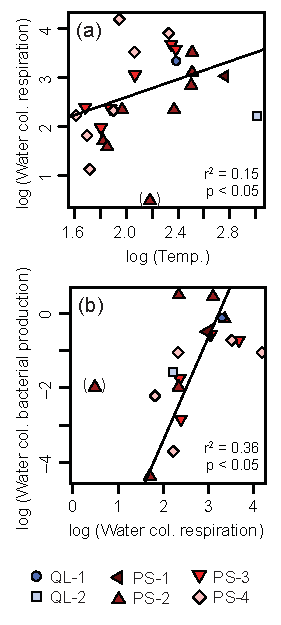
\includegraphics[width=.38\textwidth]{Fig_2-4.pdf}
\captionsetup{font={footnotesize}}
\caption[Relationships between variables transformed by natural logarithm.]{Relationships between variables transformed by natural logarithm. (a) Water column respiration (\emph{WCR}; mg C m\textsuperscript{-3} d\textsuperscript{-1}) versus temperature ($^{\circ}$C). (b) Water column bacterial production (\emph{BP\textsubscript{wc}}; mg C m\textsuperscript{-3} d\textsuperscript{-1}) versus \emph{WCR}. The scatterplots were created using \emph{WCR} and \emph{BP\textsubscript{wc}} data pooled from all stations. In \autoref{fig:c2n4}a, the linear regression \emph{y} = 0.91 ($\pm$0.40) \emph{x} + 0.76 ($\pm$0.88) (black line) was fitted using a weighted ordinary least squares method. In \autoref{fig:c2n4}b, we fitted the linear regression \emph{y} = 2.76 ($\pm$0.42) \emph{x}  - 8.93 ($\pm$1.19) using a type II (major axis---orthogonal distance) method to account for the uncertainties in both variables. We excluded from both regressions the outlier set off with parentheses. Colors and symbols for the various stations correspond to those used in \autoref{fig:c2n2} and \autoref{fig:c2n3}. \emph{WCR} and \emph{BP\textsubscript{wc}} were converted to units of carbon using the same conventions as in \autoref{fig:c2n3}. Uncertainties on regression parameters are $\pm$ 1$\sigma$.}
\label{fig:c2n4}
\end{SCfigure}

The substrate-specific respiration rates we measured on sinking particle material (\emph{k\textsubscript{R}}) spanned an order of magnitude (\autoref{table:c2n2}) and exhibited no clear relationship with depth, water temperature, water column respiration or bacterial production rates, or the magnitude or bulk quality (i.e., rain ratio) of the particulate C flux. The range of values we obtained for \emph{k\textsubscript{R}} (0.007 $\pm$ 0.003 to 0.173 $\pm$ 0.105 d\textsuperscript{-1}) was broader than, yet with a median similar to, the range reported by Sarmiento and Gruber (2006) for \emph{k}\textsubscript{remin}, a model-diagnosed rate constant that encompassed both respiration by particle-attached bacteria and other removal processes (0.02 to 0.1 d\textsuperscript{-1}). Iversen and Ploug (2010) reported a range of values for the carbon-specific respiration rate from 0.08 to 0.20 d\textsuperscript{-1}, based on a compilation of their own measurements and several from the literature. Using an in situ particle incubator in the Sargasso Sea (Bermuda Atlantic Time-series Study site), McDonnell et al. (2015) calculated significantly faster particle ``microbial remineralization rates'' of 0.3 $\pm$ 0.1 to 1.7 $\pm$ 0.4 d\textsuperscript{-1} by normalizing oxygen consumption directly to trap fluxes; these exceeded our sole measurement from the Sargasso (0.084 $\pm$ 0.008, at station QL-2) by an order of magnitude.

The mean value of our \emph{k\textsubscript{R}} measurements for all stations and depths (0.058 $\pm$ 0.011 d\textsuperscript{-1}; \emph{N} = 9 unique observations) agreed with the POC-specific respiration rate of 0.083 d\textsuperscript{-1} calculated by Ploug and Grossart (2000) from roller tank experiments. Working with a natural bacterial assemblage from temperate Pacific waters, Bidle et al. (2002) measured POC-specific remineralization rates on diatom detritus ranging from 0.09 to 0.28 d\textsuperscript{-1}. These rates, which encompassed both particle-attached respiration and processes related to enzymatic solubilization and mechanical disaggregation, were heavily correlated with temperature. Specific remineralization rates of the biogenic silica in the same detritus ranged from 1.1 to 49\% of the corresponding POC-specific rate.

\section{Model Results and Discussion}

\subsection{Sensitivity Analyses}

We compared our model results --- POC flux predictions based on ranges of values for \emph{k\textsubscript{S}}\textsubscript{,\emph{D},\emph{Z}} and \emph{W\textsubscript{avg}} --- to observations of POC flux at two depth intervals for each of five process stations (\autoref{fig:c2n5}). Relatively narrow confidence regions in 6 of our 10 analyses allowed us to place both upper and lower constraints on the agreement between our predictions and observations (\autoref{fig:c2n5}; confidence regions are shaded and enclosed within dashed lines). However, in four cases (both depth intervals at station QL-1, the 150-300 m interval at PS-2, and the 50-150 m interval at PS-4), large uncertainties in either the observed fluxes or in our inputs of \emph{k\textsubscript{R}} prevented us from assigning significance to the model-observed deviations, except at very slow sinking speeds. The six analyses that produced narrower confidence regions offer several insights into the partitioning between processes that drive particle flux attenuation (\autoref{sssec:Partitioning of Sinking POC Flux Attenuation Between Direct Bacterial Respiration and Other Degradation Processes}, below).

\subsubsection{Minimum Constraints on Average Particle Sinking Velocity}
\label{sssec:Minimum Constraints on Average Particle Sinking Velocity}

We diagnosed a statistically significant minimum constraint on \emph{W\textsubscript{avg}} at all depth intervals to which we applied a sensitivity analysis (\autoref{table:c2n3}). At slow average sinking velocities (\autoref{fig:c2n5}, to extreme left in each plot), we obtained low uncertainties from the model over the entire range of values we considered for \emph{k\textsubscript{S}}\textsubscript{,\emph{D},\emph{Z}}; this allowed us to exclude completely from the solution space values of \emph{W\textsubscript{avg}} that fell below a certain threshold. The minimum bound on \emph{W\textsubscript{avg}} we obtained in this manner ranged from 2.8 m d\textsuperscript{-1} to 16.8 m d\textsuperscript{-1} (mean $\pm$ standard deviation, 9.3 $\pm$ 4.3 m d\textsuperscript{-1}). There was no statistically significant difference between the average minimum bounds for the two depth intervals.

While the form of our analysis did not allow us to estimate a central, best fit value for \emph{W\textsubscript{avg}} at each station, the minimum constraints we obtained are consistent with previous observations of the average particle sinking velocity at a diversity of sites in the mesopelagic North Atlantic Ocean (\autoref{table:acn1}). Although sinking velocities \textless{} 1 m d\textsuperscript{-1} have been reported for cell material from individual cultures of certain phytoplankton species (Bach et al., 2012) and for certain lithogenic particles of Aeolian origin (Ohnemus and Lam, 2014), a median \emph{W\textsubscript{avg}} of 50 m d\textsuperscript{-1} (interquartile range, 11.5--100 m d\textsuperscript{-1}; mean, 63.8 m d\textsuperscript{-1}) emerged from a data set of observations we assembled from the literature for the temperate North Atlantic Ocean at depths \textless{} 1000 m (\autoref{table:acn1} and \autoref{fig:c2n5}). Average particle sinking velocities well in excess of 500 m d\textsuperscript{-1} have been reported in other ocean basins and at depths \textgreater{} 1500 m (Berelson, 2002; McDonnell et al., 2015; Stemmann et al., 2004a). In instances where a bimodal distribution of particle sinking velocities has been observed in the North Atlantic, a slow-sinking particle size fraction can be complemented by a fast-sinking fraction with an average sinking velocity of nearly 200 m d\textsuperscript{-1} (Riley et al., 2012). Of course, regardless of the system, \emph{W\textsubscript{avg}} is a function of a heterogeneous distribution of individual sinking speeds attached to different particle size classes (McDonnell and Buesseler, 2010; Villa-Alfageme et al., 2014). Despite the lack of correlation in this case between \emph{k\textsubscript{R}} and the ratio of POC:PIC in the sinking flux (i.e., the rain ratio; \autoref{table:c2n2}), we did identify a weak (\emph{r}\textsuperscript{2} = 0.19) and barely significant (\emph{p} = 0.1) negative correlation between our minimum estimates of \emph{W\textsubscript{avg}} and the rain ratio. This result follows the finding of a recent, culture-based laboratory study suggesting concentrations of biogenic PIC can enhance bulk particle sinking speed even when little effect is seen on the substrate-specific respiration rate (Iversen and Ploug, 2010). Conversely, Lam et al. (2011) have suggested that the high mesopelagic transfer efficiencies associated with CaCO\textsubscript{3}-rich organic matter may be less a function of faster sinking velocity than the result of an inherent complexity in such organic matter that renders it less amenable to direct respiration.

\subsubsection{Partitioning of Sinking POC Flux Attenuation Between Direct Bacterial Respiration and Other Degradation Processes}
\label{sssec:Partitioning of Sinking POC Flux Attenuation Between Direct Bacterial Respiration and Other Degradation Processes}

Several sets of values of \emph{W\textsubscript{avg}} and \emph{k\textsubscript{S}}\textsubscript{,\emph{D},\emph{Z}} minimized the deviation between the modeled and observed fluxes at each station; these are the pairs of values that fall along the ``0'' isoline in each of the plots in \autoref{fig:c2n5}. To constrain this set of possible solutions and obtain best fit estimates for \emph{k\textsubscript{S}}\textsubscript{,\emph{D},\emph{Z}} in each case, we sought to limit our assessment of \emph{k\textsubscript{S}}\textsubscript{,\emph{D},\emph{Z}} to those values of \emph{W\textsubscript{avg}} that were most plausible for the North Atlantic. We chose 50 m d\textsuperscript{-1}, the median value of the data set we assembled from the literature (\autoref{fig:c2n5} and \autoref{table:acn1}; \emph{N} = 72 individual observations of \emph{W\textsubscript{avg}}), as the average sinking velocity for which we report a best fit value for \emph{k\textsubscript{S}}\textsubscript{,\emph{D},\emph{Z}} in each case. Using this criterion, we obtained estimates of \emph{k\textsubscript{S}}\textsubscript{,\emph{D},\emph{Z}} and accompanying uncertainties of $0.015_{ - 0.02}^{ + 0.15}$ to $0.57_{ - 0.30}^{ + 0.43}$ d\textsuperscript{-1} (\autoref{table:c2n3}; mean $\pm$ standard deviation, 0.16 $\pm$ 0.17 d\textsuperscript{-1}). These estimates are the values in \autoref{fig:c2n5} (denoted with + symbol) where the vertical line corresponding to 50 m d\textsuperscript{-1} intersects the $\Delta$(model-observed) ``0'' isoline and the boundaries of the confidence region. To estimate the relative contribution to sinking POC flux attenuation of the processes represented in \emph{k\textsubscript{S}}\textsubscript{,\emph{D},\emph{Z}} compared with respiration of particle material by attached bacteria, we calculated the ratio of the two rate constants, \emph{k\textsubscript{S}}\textsubscript{,\emph{D},\emph{Z}} : \emph{k\textsubscript{R}}. This ratio ranged from 0.3 over the 50--150 m interval at station PS-4 to 11.2 over the same interval at station PS-2. The mean ratio of the two rate constants was 3.4, although the distribution was highly scattered (standard deviation = 4.0).

\begin{figure}[!p]
\includegraphics[width=1\textwidth]{Fig_2-5.pdf}
\end{figure}

In the following sense, we believe these values represent a conservative estimate of the predominance of other degradation processes over the respiration of sinking particles by attached bacteria. Our diagnostic approach depends on the value we assume for \emph{W\textsubscript{avg}}; we applied the median value of 50 m d\textsuperscript{-1} from our survey of the literature. If the true average sinking velocity at any station were faster than 50 m d\textsuperscript{-1}, we would therefore have underestimated \emph{k\textsubscript{S}}\textsubscript{,\emph{D},\emph{Z}} (and, by extension, the ratio of \emph{k\textsubscript{S}}\textsubscript{,\emph{D},\emph{Z}} : \emph{k\textsubscript{R}}). We suspect the average sinking velocity at our sites could well have been faster, particularly at the stations where primary production was dominated by coccolithophores (PS-3 and PS-4; \autoref{table:c2n2}). The one study in our literature survey to report average sinking velocities for particles specifically associated with a coccolithophore bloom estimated a \emph{W\textsubscript{avg}} of 141 $\pm$ 11 m d\textsuperscript{-1}, nearly 3 times that of the 50 m d\textsuperscript{-1} we selected (Knappertsbusch and Brummer, 1995). During a summer coccolithophore bloom in the equatorial Atlantic, Fischer and Karakas (2009) measured average particle sinking velocities of almost 570 m d\textsuperscript{-1}. Given the shapes of the curves that result from the exponential decay model, a small upward revision in \emph{W\textsubscript{avg}} from a starting value of 50 m d\textsuperscript{-1} would have little impact on our diagnosis. For example, in all instances except for the 150--300 m depth interval at station QL-1, an increase in \emph{W\textsubscript{avg}} from 50 to 75 m d\textsuperscript{-1} would produce only a modest change in the value of \emph{k\textsubscript{S}}\textsubscript{,\emph{D},\emph{Z}}, since this is region where the ``0'' isoline curve begins to approach an asymptote (\autoref{fig:c2n5}).
\begin{figure} [!t]
\captionsetup{font={footnotesize}}
\captionof{figure}[Sensitivity analyses of the particle flux attenuation model by station and depth interval.]{(preceding page). Sensitivity analyses of the particle flux attenuation model by station and depth interval. We evaluated variation in two parameters, the average particle sinking velocity (\emph{W\textsubscript{avg}}, from 1 to 200 m d\textsuperscript{-1}; \emph{x}-axis) and \emph{k\textsubscript{S}}\textsubscript{,\emph{D},\emph{Z}}, an activity constant that captures losses of sinking POC due to processes other than direct respiration by particle-attached bacteria (\emph{y}-axis; from 10\textsuperscript{-5} to 1 d\textsuperscript{-1}; \autoref{fig:c2n1}). Colorbar ramp and labeled contour lines indicate, for a given pair of values of \emph{W\textsubscript{avg}} and \emph{k\textsubscript{S}}\textsubscript{,\emph{D},\emph{Z}}, deviation of the model result from the observed POC flux at that station, in units of mg C m\textsuperscript{-2} d\textsuperscript{-1}. Left panels: Results for 50-150 m. Right panels: Results for 150-300 m. The secondary \emph{y}-axis (ratio of \emph{k\textsubscript{S}}\textsubscript{,\emph{D},\emph{Z}} to \emph{k\textsubscript{R}}, the measured substrate-specific rate of respiration on sinking particles) shows the relative contribution to particle flux attenuation at each station by respiration compared to the other processes that degrade sinking particles. The shaded area in each plot encompassed by the dashed line is a 1$\sigma$ ({\raise.17ex\hbox{$\scriptstyle\sim$}} 68\%) confidence region derived from uncertainties in the model solutions and observed flux at that station. Model-observed deviations outside this region are statistically significant. Also shown above each set of plots is an identical histogram of relevant observations (\emph{N} = 72) of average sinking velocities in the North Atlantic; the assembly of these data is described in \autoref{sssec:Minimum Constraints on Average Particle Sinking Velocity} of the text. The median (50 m d\textsuperscript{-1}; band at center of box plot) and IQR (11.5-100 m d\textsuperscript{-1}) are shown in the accompanying boxplot. Whiskers extend to 1.5 IQR. The sole reported value \textgreater{} 200 m d\textsuperscript{-1} (250 m d\textsuperscript{-1}) was excluded as an outlier.}
\label{fig:c2n5}
\end{figure}

We take the results of our analysis to indicate that, at minimum, the majority of sinking particle material attenuated between 50 and 300 m did not meet its ultimate fate through direct respiration by attached bacteria. Instead, the results suggest a significant fraction of the sinking particulate flux was transferred to the water column as suspended particulate or dissolved organic matter, at least some of it providing a metabolic subsidy to the free-living bacterial community. Because some of the sinking POC flux might have been directly respired by associated zooplankton, we cannot be certain \emph{k\textsubscript{S}}\textsubscript{,\emph{D},\emph{Z}} exclusively represents the transfer of mass to the water column. However, while carbon demand incurred by zooplankton is an important sink in some marine systems such as the central equatorial Pacific (Landry et al., 1997), subarctic Pacific (Steinberg et al., 2008b), and at station ALOHA (Steinberg et al., 2008a), the results of the North Atlantic Bloom Experiment suggest zooplankton are much less significant players in midlatitude or subpolar North Atlantic systems during bloom conditions (Dam et al., 1993). In this case, we hypothesize that the major role played by zooplankton was instead that of mechanical disaggregator, complementing enzymatic solubilization by particle-attached bacteria in transferring carbon to the dissolved and suspended particulate phases.

The hypothesized transfer of organic matter from the sinking particulate to suspended or dissolved phases is supported by theoretical and laboratory studies (Alldredge, 2000; Bendtsen et al., 2002; Grossart and Simon, 1998; Ki\o{}rboe and Jackson, 2001), evidence from other field-based research (Giering et al., 2014; Smith et al., 1992; Taylor and Karl, 1991), and, at stations PS-2, PS-3, and PS-4, by very high rates of depth-integrated water column respiration from 50 to 150 m (465.2 $\pm$ 182.1 to 887.09 $\pm$ 456.2 mg C m\textsuperscript{-2} d\textsuperscript{-1}; mean $\pm$ standard deviation, 729.3 $\pm$ 266.0 mg C m\textsuperscript{-2} d\textsuperscript{-1}; \autoref{table:c2n3}). Intriguingly, we could find no direct statistical correlations between our estimates of the \emph{k\textsubscript{S}}\textsubscript{,\emph{D},\emph{Z}} : \emph{k\textsubscript{R}} ratio (or \emph{k\textsubscript{S}}\textsubscript{,\emph{D},\emph{Z}} itself) and any of the other parameters we measured. In the cases of \emph{BP\textsubscript{wc}}, \emph{WCR}\textsubscript{int}, and \emph{BGE}\textsubscript{pa} specifically, we did not have enough observations of the parameters to make a statistical assessment (\autoref{table:c2n2} and \autoref{table:c2n3}).

While our analysis did not allow us to identify the specific mechanisms by which this mass transfer might have occurred, our finding is general in nature and therefore accommodates all of the degradation processes we considered in our initial conceptualization of particle flux attenuation (\autoref{fig:c2n1}). In balancing a carbon budget for a site roughly 1000 km southeast of our PS-2 station, Giering et al. (2014) hypothesized that mechanical fragmentation by zooplankton had diverted nearly a third of fast-sinking particles to the dissolved and suspended phases, where the carbon they contained was then respired by bacteria. Mayor et al. (2014) described this apparent dynamic as a manifestation of Fenchel's (1970) ``microbial gardening'' hypothesis. Because so much of the sinking POC appeared to meet its ultimate fate in the water column, Giering et al. chose to construct their budget around indirect estimates of the depth-integrated water column respiration rate, which they contended best captured the total metabolic sink imposed by the microbial community.

Drawing on observations from the North Pacific, Taylor and Karl (1991) concluded that the inefficient metabolism of sinking particles by attached microbiota was likely reflected in a large transfer of organic matter to the suspended and dissolved phases. This is the roughly the same hypothesis advanced by Smith et al. (1992), who based their speculation on the very intense ectohydrolytic enzyme activity and low direct carbon demand they measured on sinking particle material. Other authors have also used observations and manipulations of particle material to argue for the importance of this mechanism in carbon transfer (Alldredge, 2000; Grossart and Simon, 1998). Ki\o{}rboe and Jackson (2001) later used results from a series of models to estimate that the dissolved organic matter left behind in the wake of a sinking particle could provide a very significant subsidy to the surrounding water column; Bendtsen et al\emph{.} (2002) concluded based on a larger-scale modeling analysis that solubilization of particle material was a significant source of DOC in the deep ocean.

In invoking this mechanism as a possible explanation for their findings, Taylor and Karl (1991) noted that any form of disaggregation or solubilization necessarily introduces a time lag between components of the ecosystem metabolic engine. The sinking organic matter not directly respired by attached bacteria --- as we hypothesize, a majority, or at least a significant fraction, of the sinking POC at our sites --- will not necessarily become immediate metabolic substrate for microbes in the water column. Consistent with observations from a variety of marine systems (see our brief discussion in \autoref{ssec:Bacterial Production}, above), this DOM or suspended POM may linger for weeks, months, or years before it is respired; some fraction will become part of the recalcitrant dissolved organic matter pool. Solubilization of sinking particles and the fraction of solubilized material that is directly respired by attached bacteria are therefore directly intertwined, even when the majority of the solubilized material is instead transferred to the water column.

Ki\o{}rboe et al. (2002) have further suggested that some loss of sinking particle mass can be explained by the shedding of live bacterial cells, which abandon the particle for the water column. Given the low bacterial growth efficiencies we observed on both sinking particles and in the water column (\autoref{table:c2n2}), we suspect this mechanism of particle loss was probably not significant in the present study.

\subsubsection{Enigmatically Low Efficiencies of Bacterial Growth}
\label{sssec:Enigmatically Low Efficiencies of Bacterial Growth}

We used our observations of water column bacterial production and respiration to calculate the water column \emph{BGE} (\emph{BGE\textsubscript{wc}}) at stations PS-2, PS-3, and PS-4 (\autoref{table:c2n2}). At stations QL-1 and QL-2, complementary measurements allowed us to calculate analogous values on sinking particles (\autoref{table:c2n2}). Bacterial growth in both carbon reservoirs proved generally inefficient, but our estimates of \emph{BGE} in the water column at depths $\geq$ 50 m were extraordinary low (0.001 $\pm$ 0.001 to 0.014 $\pm$ 0.012; mean $\pm$ standard deviation, 0.006 $\pm$ 0.002). Estimates of \emph{BGE\textsubscript{wc}} as low as 0.001 have been reported for depths below the mixed layer (90 m) in the highly oligotrophic Mediterranean Sea (Lem\'{e}e et al., 2002), and Reinthaler et al. (2006) reported growth efficiencies of just 0.006-0.016 in deep waters (\textgreater{}1200 m) of the North Atlantic. By contrast, \emph{BGE}s of 0.09 to 0.38 were estimated for the Ross Sea surface layer during a bloom of \emph{Phaeocystis} (Carlson et al., 1999). However, in the latter case, one might expect that the substrate available to the bacterial community was considerably more amenable to metabolism than either the sinking particles or the dissolved and suspended organic matter derived from them.

We believe for several reasons that our estimates are minimum bounds on water column \emph{BGE}. Since we used unfiltered water samples in our incubations, constituents of the water column microbial community other than prokaryotes (nanozooplankton, protists, and even some phytoplankton) could have contributed to the observed consumption of oxygen if they were present. Although we controlled for the presence of macrozooplankton by visual inspection, Ki\o{}rboe (2001) notes that it is virtually impossible to distinguish between bacteria and other smaller microorganisms such as protozoans. If we assume conservatively that these other organisms contributed as much to respiration as did bacteria, our mean estimate of \emph{BGE\textsubscript{wc}} for depths $\geq$ 50 m would roughly double to 0.01 $\pm$ 0.004. Additionally, flaws inherent in the \textsuperscript{3}H-leucine incorporation method, or in our choice of values for \emph{ID} or $\nu _{C:leu}$, could have caused us to significantly underestimate rates of bacterial production. The large uncertainties we introduced into our estimates of depth-integrated BP when we considered variation in both of the conversion factors (uncertainties represented 60\%, on average, of the accompanying estimate; \autoref{table:c2n3}) demonstrate how a broad range of possible values can be extrapolated from a single set of leucine incorporation measurements. For example, if we also discarded our conservative assumption for \emph{ID} and instead adopted a value of 2 --- assuming bacteria incorporated as much radiolabeled leucine into protein as endogenous leucine (Kirchman, 2001) --- our mean estimate of \emph{BGE\textsubscript{wc}} could be as high as 0.04.

However, the fact remains that when considered independently, our observations of both bacterial production and water column respiration are highly consistent with the large sets of values previously reported for the North Atlantic for both parameters. Critically, even a \emph{BGE} of 0.04 --- the highest possible value we could accept obtaining from our observations under the hypothetical scenario above --- would still be considerably lower than the 0.15 applied by Steinberg et al. (2008b) or the median value of 0.08 Giering et al. (2014) obtained from an assembled data set; those studies represent two of the most prominent attempts to balance carbon budgets in the mesopelagic ocean on an ecosystem scale.

\subsubsection{Possible Imbalances in the North Atlantic Carbon Budget}

If, as Giering et al. (2014) and others have contended, depth-integrated water column bacterial respiration is the primary carbon sink in a given marine ecosystem, our data suggest a very substantial imbalance existed in the carbon budgets of our study sites, at least over the spatial and temporal scales we considered. At the three stations (PS-2, PS-3, and PS-4) for which we had concurrent measurements of the relevant parameters, the metabolic sink imposed by \emph{WCR\textsubscript{int}} over the 50 to 150 m depth interval surpassed observed attenuation in sinking POC flux over the same interval by an average of more than 26 times (\autoref{table:c2n3}). There are very few sediment trap- or \textsuperscript{234}Th-derived observations of POC fluxes in the literature that would have supplied a quantity of carbon sufficient to satisfy the respiratory demand we measured; for example, the 940.4 mg C m\textsuperscript{-2} d\textsuperscript{-1} observed by Le Moigne et al., 2015) in the Atlantic sector of the Arctic Ocean is remarkably high. No observations previously reported for the sub-Arctic North Atlantic would have satisfied the metabolic demand imposed by our observations of \emph{WCR\textsubscript{int}}.

Depth-integrated water column BP comprised such a small fraction of \emph{WCR\textsubscript{int}} at each site (\autoref{table:c2n3}) that the substantial uncertainties we introduced into our calculations of \emph{BP\textsubscript{int}} by incorporating variation in \emph{ID} and $\nu _{C:leu}$ were of relatively little consequence. Our bootstrap analysis indicated that variation in the two conversion factors accounted for more than 90\% of the uncertainties in our estimates of \emph{BP\textsubscript{int}}. We acknowledge here that, if instead of measuring respiration directly, we had extrapolated estimates of \emph{WCR\textsubscript{int}} from these measurements of BP (as did Giering et al. (2014)), these uncertainties would have become extremely consequential. Further, if some systematic bias in our incubation technique caused us to overestimate individual rates of \emph{WCR} by even a small amount, the offset would have produced a large positive deviation upon vertical integration.

Even if our calculations of \emph{WCR\textsubscript{int}} represented a twofold overestimate of the metabolic demand imposed by bacteria (based on the same logic we invoke in our discussion of \emph{BGE}; \autoref{sssec:Enigmatically Low Efficiencies of Bacterial Growth}, above), the carbon budgets at these three sites could only be closed by large lateral or vertical inputs of DOC, or by some other unknown source of reducing power. Zooplankton respiration in the water column --- a sink we did not measure or estimate --- would supply additional oxidizing power in excess of that already captured in \emph{WCR\textsubscript{int}}, creating a demand for even more reduced carbon. Giering et al. estimated that inputs of DOC supplied 17\% of the carbon needed to balance the metabolic budget they created in their study; similar values have been reported elsewhere in the North Atlantic (Carlson et al., 2010), though evidence suggests the fraction of export supplied by DOC could be even higher ($\sim 29$\%) in oligotrophic waters of the Sargasso Sea (Carlson et al., 1994). Inputs of DOC on the order of that observed in those studies could narrow the metabolic disparity at our sites significantly, but would be insufficient to close the gap completely.

Alternatively, our bottle-based measurements of \emph{WCR\textsubscript{int}} could be significant overestimates that reflect a methodological bias. Bottle-based methods for measuring respiration or other metabolic processes in marine microorganisms are prone to error from (1) contamination and disruption introduced through the process of obtaining seawater samples and preparing them for incubation, including the effects of depressurization when samples are collected from depth (Tamburini et al., 2013); (2) unrepresentative incubation conditions that do not faithfully reproduce the variations in temperature and light inherent in natural systems; and (3) so-called ``bottle effects'' associated with low-volume incubations which may limit nutrient availability (Furnas, 2002) or induce unnatural changes in community structure (Calvo-D\'{i}az et al., 2011; Venrick et al., 1977).

Our data thus suggest balance in the North Atlantic carbon budget remains elusive, likely due to some combination methodological limitations, a failure to account for some critical additional flux, or a failure to consider adequately the time scales of those sources and sinks we did measure. Despite a handful of successful attempts at balancing marine carbon budgets on ecosystem (Giering et al., 2014) and basin scales (Williams et al., 2013), we arrive by different methods at the same vexing problem that confronted Steinberg et al. (2008b): A system that apparently out of metabolic balance. This imbalance notwithstanding, the strong oxidizing power in the depth-integrated respiration rates we observed still supports our hypothesis for a significant transfer of sinking particulate carbon to the water column. Insofar as this mass transfer is concerned, the apparent metabolic imbalance simply indicates that carbon evolved from sinking particle material is alone insufficient to supply the necessary reducing power.

\section{Conclusion}

The relative strength --- and apparent predominance, at the majority of sites in this study --- of the other biological and mechanical processes that compete with direct respiration to degrade sinking particles suggest the mesopelagic ocean is characterized by a distinct remineralization regime in which hydrolysis and respiration are significantly decoupled. Sinking organic matter transferred to the dissolved or suspended particulate phases through enzymatic solubilization or mechanical disaggregation provides a considerable metabolic subsidy to the water column microbial community. Yet evidence from other studies suggests the respiration of this organic matter may lag its transfer from the sinking particulate phase by weeks, months, or years. This temporal disconnect makes it difficult to diagnose the exact mechanisms of organic matter transfer from the sinking particulate phase and hinders accurate appraisal of the flux's magnitude.

The large disparity we documented between rates of depth-integrated water column respiration and attenuation of sinking POC is further evidence that our methods of characterizing microbial metabolisms remain inadequate, or that our knowledge of the various reservoirs and fluxes that define the marine carbon cycle remains incomplete. The very low bacterial growth efficiencies we observed in this study are further evidence for both of these deficiencies. The variation in \emph{BGE} we observed both in the water column and on the sinking particles suggests that the lability of particulate organic matter can be altered as it is exported to depth.

One way to diagnose apparent carbon budget discrepancies is by pairing incubation-based techniques such as those we employed with concurrent measurements based on in situ geochemical tracer techniques that integrate more broadly over both time and space (e.g., Quay et al., 2010). For example, at steady state, a respiratory sink of the magnitude we measured would have required some complementary source of dissolved oxygen; otherwise, we would have expected to observe at some timescale a significant decrease in dissolved oxygen inventory. Concurrent measurements of dissolved oxygen anomalies (e.g., Najjar and Keeling, 1997) or apparent oxygen utilization (e.g., Stanley et al., 2012) might have allowed us to determine whether this metabolic demand was in fact balanced over seasonal or annual timescales by other processes.

Despite a handful of recent studies that have successfully balanced carbon budgets for sectors of the North Atlantic, we find strong justification here for the further development of new analytical methods and new hypotheses about how the carbon cycle functions. At the same time, the rates of water column respiration that drove this apparent imbalance provide support for our hypothesis that degradation processes other than direct respiration can dominate particle flux attenuation. Investigators seeking to accurately characterize the marine carbon cycle with new mechanistic models of production and export should endeavor to incorporate these other processes to an extent equal to that of respiration.

\section{Acknowledgments}

We thank the captains and crew of the R/V \emph{Knorr}, as well as Jamey Fulton, Anton Zafereo, David Sims, Filipa Carvalho, Helen Fredricks, Dan McCorkle, Valier Galy, Krista Longnecker, Suni Shah, Dave Glover, Carl Johnson, Olivia De Meo, Steve Manganini, Phoebe Lam, Joe Salisbury, and Maria Kavanaugh. Elizabeth Kujawinski provided thoughtful comments on an earlier version of the manuscript. We are lastly grateful to Hugh Ducklow and to two anonymous reviewers, whose criticism improved the manuscript dramatically. J.R.C. acknowledges support from a U.S. Environmental Protection Agency (EPA) STAR Graduate Fellowship (Fellowship Assistance agreement FP-91744301-0). The contents of this research have not been formally reviewed by EPA. The views expressed in this manuscript are solely those of the authors, and EPA does not endorse any products or commercial services mentioned therein. K.D.B. acknowledges support from the National Science Foundation (NSF OCE-1061883) and the Gordon and Betty Moore Foundation (3301 and 3789). S.C.D. acknowledges support from the National Science Foundation through the Center for Microbial Oceanography: Research and Education (C-MORE) (NSF EF-0424599). B.A.S.V.M. acknowledges support from the National Science Foundation (NSF OCE-1155438, OCE-1059884, and OCE-1031143), the Gordon and Betty Moore Foundation, and the Woods Hole Oceanographic Institution through a Cecil and Ida Green Foundation Innovative Technology Award and an Interdisciplinary Science Award.

\section{Availability of Data and Code }

Curated oceanographic data can be found on the BCO-DMO web site at \url{http://www.bco-dmo.org/deployment/58787} (KN207-1) and \url{http://www.bco-dmo.org/project/2136} (KN207-3). Additional data and all code used to produce the figures and analysis in this chapter are contained in GitHub repositories at \texttt{\href{https://github.com/jamesrco/MultipleFatesofParticles}{https://github.com/jamesrco/MultipleF\\atesofParticles}} and (for analysis of bacterial production data) \url{https://github.com/jamesrco/3H_Leu_BactProd}

\clearpage
\begin{singlespace}
\section*{References}
\addtocounter{section}{1}
{\setlength{\parindent}{0pt}
Alldredge, A. L. (2000), Interstitial dissolved organic carbon (DOC) concentrations within sinking marine aggregates and their potential contribution to carbon flux, \emph{Limnology \& Oceanography}, 45(6), 1245-1253.

{\setlength{\parskip}{10pt}

Alldredge, A. L., T. C. Granata, C. C. Gotschalk, and T. D. Dickey (1990), The physical strength of marine snow and its implications for particle disaggregation in the ocean, \emph{Limnology \& Oceanography}, 35(7), 1415-1428.

Alonso-Saez, L., et al. (2008), Factors controlling the year-round variability in carbon flux through bacteria in a coastal marine system, \emph{Ecosystems}, 11(3), 397-409, doi:\href{http://dx.doi.org/10.1007/S10021-008-9129-0}{10.1007/S10021-008-9129-0}.

Anderson, L. A., and J. L. Sarmiento (1994), Redfield ratios of remineralization determined by nutrient data-analysis, \emph{Global Biogeochemical Cycles}, 8(1), 65-80, doi:\href{http://dx.doi.org/10.1029/93GB03318}{10.1029/93GB03318}.

Anderson, T. R., and K. W. Tang (2010), Carbon cycling and POC turnover in the mesopelagic zone of the ocean: Insights from a simple model, \emph{Deep Sea Research Part II: Topical Studies in Oceanography}, 57(16), 1581-1592, doi:\href{http://dx.doi.org/10.1016/j.dsr2.2010.02.024}{10.1016/j.dsr2.2010.02.024}.

Aranguren-Gassis, M., P. Serret, E. Fern\'{a}ndez, J. L. Herrera, J. F. Dom\'{i}nguez, V. P\'{e}rez, and J. Escanez (2012), Balanced plankton net community metabolism in the oligotrophic North Atlantic subtropical gyre from Lagrangian observations, \emph{Deep Sea Research Part I: Oceanographic Research Papers}, 68, 116-122, doi:\href{http://dx.doi.org/10.1016/j.dsr.2012.06.004}{10.1016/j.dsr.2012.06.004}.

Azam, F. (1998), Microbial control of oceanic carbon flux: The plot thickens, \emph{Science}, 280(5364), 694-696, doi:\href{http://dx.doi.org/10.1126/science.280.5364.694}{10.1126/science.280.5364.694}.

Azam, F., and F. Malfatti (2007), Microbial structuring of marine ecosystems, \emph{Nature Reviews Microbiology}, 5(10), 782-791.

Azam, F., D. C. Smith, G. F. Steward, and \AA{}. Hagstr\"{o}m (1994), Bacteria-organic matter coupling and its significance for oceanic carbon cycling, \emph{Microbial Ecology}, 28(2), 167-179, doi:\href{http://dx.doi.org/10.1007/BF00166806}{10.1007/BF00166806}.

Bach, L. T., U. Riebesell, S. Sett, S. Febiri, P. Rzepka, and K. G. Schulz (2012), An approach for particle sinking velocity measurements in the 3-400 $\mu$m size range and considerations on the effect of temperature on sinking rates, \emph{Marine Biology}, 159(8), 1853-1864, doi:\href{http://dx.doi.org/10.1007/S00227-012-1945-2}{10.1007/S00227-012-1945-2}.

Bendtsen, J., C. Lundsgaard, M. Middelboe, and D. Archer (2002), Influence of bacterial uptake on deep-ocean dissolved organic carbon, \emph{Global Biogeochemical Cycles}, 16(4), 1127, doi:\href{http://dx.doi.org/10.1029/2002GB001947}{10.1029/2002GB001947}.

Berelson, W. M. (2002), Particle settling rates increase with depth in the ocean, \emph{Deep Sea Research Part II: Topical Studies in Oceanography}, 49(1-3), 237-251.

Bidle, K. D., M. Manganelli, and F. Azam (2002), Regulation of oceanic silicon and carbon preservation by temperature control on bacteria, \emph{Science}, 298(5600), 1980-1984, doi:\href{http://dx.doi.org/10.1126/science.1076076}{10.1126/\\science.1076076}.

Boyd, P. W., and T. W. Trull (2007), Understanding the export of biogenic particles in oceanic waters: Is there consensus?, \emph{Progress in Oceanography}, 72(4), 276-312, doi:\href{http://dx.doi.org/10.1016/J.Pocean.2006.10.007}{10.1016/J\\.Pocean.2006.10.007}.

Buesseler, K. O., and P. W. Boyd (2009), Shedding light on processes that control particle export and flux attenuation in the twilight zone of the open ocean, \emph{Limnology \& Oceanography}, 54(4), 1210-1232, doi:\href{http://dx.doi.org/10.4319/lo.2009.54.4.1210}{10.4319/lo.2009.54.4.1210}.

Buesseler, K. O., et al. (2007a), An assessment of the use of sediment traps for estimating upper ocean particle fluxes, \emph{Journal of Marine Research}, 65(3), 345-416.

Buesseler, K. O., et al. (2007b), Revisiting carbon flux through the ocean's twilight zone, \emph{Science}, 316(5824), 567-570, doi:\href{http://dx.doi.org/10.1126/science.1137959}{10.1126/science.1137959}.

Burd, A. B. (2013), Modeling particle aggregation using size class and size spectrum approaches, \emph{Journal of Geophysical Research: Oceans}, 118, 3431-3443, doi:\href{http://dx.doi.org/10.1002/Jgrc.20255}{10.1002/Jgrc.20255}.

Burd, A. B., et al. (2010), Assessing the apparent imbalance between geochemical and biochemical indicators of meso- and bathypelagic biological activity: What the @\$\#! is wrong with present calculations of carbon budgets?, \emph{Deep Sea Research Part II: Topical Studies in Oceanography}, 57(16), 1557-1571, doi:\href{http://dx.doi.org/10.1016/J.Dsr2.2010.02.022}{10.1016/J.Dsr2.2010.02.022}.

Calvo-D\'{i}az, A., L. D\'{i}az-P\'{e}rez, L. \'{a}. Su\'{a}rez, X. A. G. Mor\'{a}n, E. Teira, and E. Mara\~{n}\'{o}n (2011), Decrease in the autotrophic-to-heterotrophic biomass ratio of picoplankton in oligotrophic marine waters due to bottle enclosure, \emph{Applied and Environmental Microbiology}, 77(16), 5739-5746, doi:\href{http://dx.doi.org/10.1128/aem.00066-11}{10.1128/aem.00066-11}.

Carlson, C. A., H. W. Ducklow, and A. F. Michaels (1994), Annual flux of dissolved organic carbon from the euphotic zone in the northwestern Sargasso Sea, \emph{Nature}, 371(6496), 405-408.

Carlson, C. A., N. R. Bates, H. W. Ducklow, and D. A. Hansell (1999), Estimation of bacterial respiration and growth efficiency in the Ross Sea, Antarctica, \emph{Aquatic Microbial Ecology}, 19(3), 229-244, doi:\href{http://dx.doi.org/10.3354/ame019229}{10.3354/ame019229}.

Carlson, C. A., D. A. Hansell, N. B. Nelson, D. A. Siegel, W. M. Smethie, S. Khatiwala, M. M. Meyers, and E. Halewood (2010), Dissolved organic carbon export and subsequent remineralization in the mesopelagic and bathypelagic realms of the North Atlantic basin, \emph{Deep Sea Research Part II: Topical Studies in Oceanography}, 57(16), 1433-1445, doi:\href{http://dx.doi.org/10.1016/j.dsr2.2010.02.013}{10.1016/j.dsr2.2010.02.013}.

Chin-Leo, G., and D. L. Kirchman (1988), Estimating bacterial production in marine waters from the simultaneous incorporation of thymidine and leucine, \emph{Applied and Environmental Microbiology}, 54(8), 1934-1939.

Close, H. G., S. R. Shah, A. E. Ingalls, A. F. Diefendorf, E. L. Brodie, R. L. Hansman, K. H. Freeman, L. I. Aluwihare, and A. Pearson (2013), Export of submicron particulate organic matter to mesopelagic depth in an oligotrophic gyre, \emph{Proceedings of the National Academy of Sciences of the United States of America}, 110(31), 12,565-12,570, doi:\href{http://dx.doi.org/10.1073/pnas.1217514110}{10.1073/pnas.1217514110}.
 
Dam, H. G., C. A. Miller, and S. H. Jonasdottir (1993), The trophic role of mesozooplankton at 47$^{\circ}$ N, 20$^{\circ}$ W during the North-Atlantic Bloom Experiment, \emph{Deep Sea Research Part II: Topical Studies in Oceanography}, 40(1-2), 197-212, doi:\href{http://dx.doi.org/10.1016/0967-0645\%2893\%2990013-D}{10.1016/0967-0645(93)90013-D}.

del Giorgio, P. A., J. J. Cole, and A. Cimbleris (1997), Respiration rates in bacteria exceed phytoplankton production in unproductive aquatic systems, \emph{Nature}, 385(6612), 148-151.

DiTullio, G., and M. E. Geesey (2003), Photosynthetic pigments in marine algae and bacteria, in \emph{Encyclopedia of Environmental Microbiology}, vol. 5, edited by G. Bitton, pp. 2453-2470, John Wiley, New York, doi:\href{http://dx.doi.org/10.1002/0471263397.env185}{10.1002/0471263397.env185}.

Duarte, C. M., A. Regaudie-de-Giroux, J. M. Arrieta, A. Delgado-Huertas, and S. Agust\'{i} (2013), The oligotrophic ocean is heterotrophic, \emph{Annual Review of Marine Science}, 5, 551-569, doi:\href{http://dx.doi.org/10.1146/annurev-marine-121211-172337}{10.1146/annurev-marine-121211-172337}.

Ducklow, H. W., and S. C. Doney (2013), What is the metabolic state of the oligotrophic ocean? A debate, \emph{Annual Review of Marine Science}, 5, 525-533, doi:\href{http://dx.doi.org/10.1146/annurev-marine-121211-172331}{10.1146/annurev-marine-121211-172331}.

Ducklow, H. W., and S. M. Hill (1985), Tritiated-thymidine incorporation and the growth of heterotrophic bacteria in warm core rings, \emph{Limnology \& Oceanography}, 30(2), 260-272.

Ducklow, H. W., D. L. Kirchman, H. L. Quinby, C. A. Carlson, and H. G. Dam (1993), Stocks and dynamics of bacterioplankton carbon during the spring bloom in the eastern North Atlantic Ocean, \emph{Deep Sea Research Part II: Topical Studies in Oceanography}, 40(1-2), 245-263, doi:\href{http://dx.doi.org/10.1016/0967-0645\%2893\%2990016-G}{10.1016/0967-0645(93)90016-G}.

Edwards, B. R., C. M. Reddy, R. Camilli, C. A. Carmichael, K. Longnecker, and B. A. S. Van Mooy (2011), Rapid microbial respiration of oil from the Deepwater Horizon spill in offshore surface waters of the Gulf of Mexico, \emph{Environmental Research Letters}, 6(3), 03530, doi:\href{http://dx.doi.org/10.1088/1748-9326/6/3/035301}{10.1088/1748-9326/6/3/035301}.

Fenchel, T. (1970), Studies on the decomposition of organic detritus derived from the turtle grass Thalassia testudinum, \emph{Limnology \& Oceanography}, 15, 14-20.

Fischer, G., and G. Karakas (2009), Sinking rates and ballast composition of particles in the Atlantic Ocean: Implications for the organic carbon fluxes to the deep ocean, \emph{Biogeosciences}, 6(1), 85-102.

Foster, J. M., and G. B. Shimmield (2002), \textsuperscript{234}Th as a tracer of particle flux and POC export in the northern North Sea during a coccolithophore bloom, \emph{Deep Sea Research Part II: Topical Studies in Oceanography}, 49(15), 2965-2977, doi:\href{http://dx.doi.org/10.1016/S0967-0645\%2802\%2900066-8}{10.1016/S0967-0645(02)00066-8}.

Furnas, M. J. (2002), Measuring the growth rates of phytoplankton in natural populations, in \emph{Pelagic Ecology Methodology}, edited by D. V. S. Rao, pp. 221-249, A. A. Balkema, Lisse, Netherlands.

Geider, R. J. (1997), Photosynthesis or planktonic respiration?, \emph{Nature}, 388(6638), 132.

Giering, S. L. C., et al. (2014), Reconciliation of the carbon budget in the ocean's twilight zone, \emph{Nature}, 507(7493), 480-483, doi:\href{http://dx.doi.org/10.1038/nature13123}{10.1038/nature13123}.

Grossart, H. P., and M. Simon (1998), Bacterial colonization and microbial decomposition of limnetic organic aggregates (lake snow), \emph{Aquatic Microbial Ecology}, 15(2), 127-140, doi:\href{http://dx.doi.org/10.3354/Ame015127}{10.3354/Ame015127}.

Hansell, D. A., C. A. Carlson, D. J. Repeta, and R. Schlitzer (2009), Dissolved organic matter in the ocean: A controversy stimulates new insights, \emph{Oceanography}, 22(4), 202-211.

Honjo, S., J. Dymond, R. Collier, and S. J. Manganini (1995), Export production of particles to the interior of the equatorial Pacific Ocean during the 1992 EqPac experiment, \emph{Deep Sea Research Part II: Topical Studies in Oceanography}, 42(2-3), 831-870, doi:\href{http://dx.doi.org/10.1016/0967-0645\%2895\%2900034-N}{10.1016/0967-0645(95)00034-N}.

Hoppe, H.-G., K. Gocke, R. Koppe, and C. Begler (2002), Bacterial growth and primary production along a north-south transect of the Atlantic Ocean, \emph{Nature}, 416(6877), 168-171.

Iversen, M. H., and H. Ploug (2010), Ballast minerals and the sinking carbon flux in the ocean: Carbon-specific respiration rates and sinking velocity of marine snow aggregates, \emph{Biogeosciences}, 7(9), 2613-2624, doi:\href{http://dx.doi.org/10.5194/bg-7-2613-2010}{10.5194/bg-7-2613-2010}.

Jackson, G. A., and A. B. Burd (1998), Aggregation in the marine environment, \emph{Environmental Science \& Technology}, 32(19), 2805-2814, doi:\href{http://dx.doi.org/10.1021/es980251w}{10.1021/es980251w}.

Ki\o{}rboe, T. (2001), Formation and fate of marine snow: Small-scale processes with large-scale implications, \emph{Scientia Marina}, 65, 57-71.

Ki\o{}rboe, T., and G. A. Jackson (2001), Marine snow, organic solute plumes, and optimal chemosensory behavior of bacteria, \emph{Limnology \& Oceanography}, 46(6), 1309-1318.

Ki\o{}rboe, T., H.-P. Grossart, H. Ploug, and K. Tang (2002), Mechanisms and rates of bacterial colonization of sinking aggregates, \emph{Applied and Environmental Microbiology}, 68(8), 3996-4006, doi:\href{http://dx.doi.org/10.1128/aem.68.8.3996-4006.2002}{10.1128/aem.68.8.3996-4006.2002}.

Kirchman, D. (2001), Measuring bacterial biomass production and growth rates from leucine incorporation in natural aquatic environments, in \emph{Methods in Microbiology}, edited by J. H. Paul, pp. 227-237, Academic, St. Petersburg, Fla., doi:\href{http://dx.doi.org/10.1016/S0580-9517\%2801\%2930047-8}{10.1016/S0580-9517(01)30047-8}.

Knappertsbusch, M., and G. J. A. Brummer (1995), A sediment trap investigation of sinking coccolithophorids in the North Atlantic, \emph{Deep Sea Research Part I: Oceanographic Research Papers}, 42(7), 1083-1109, doi:\href{http://dx.doi.org/10.1016/0967-0637\%2895\%2900036-6}{10.1016/0967-0637(95)00036-6}.

Lam, P. J., S. C. Doney, and J. K. B. Bishop (2011), The dynamic ocean biological pump: Insights from a global compilation of particulate organic carbon, CaCO$_3$, and opal concentration profiles from the mesopelagic, \emph{Global Biogeochemical Cycles}, 25, GB3009, doi:\href{http://dx.doi.org/10.1029/2010GB003868}{10.1029/2010GB003868}.

Lamborg, C. H., K. O. Buesseler, J. Valdes, C. H. Bertrand, R. Bidigare, S. Manganini, S. Pike, D. Steinberg, T. Trull, and S. Wilson (2008), The flux of bio- and lithogenic material associated with sinking particles in the mesopelagic ``twilight zone'' of the northwest and North Central Pacific Ocean, \emph{Deep Sea Research Part II: Topical Studies in Oceanography}, 55(14-15), 1540-1563, doi:\href{http://dx.doi.org/10.1016/j.dsr2.2008.04.011}{10.1016/j.dsr2.2008.04.011}.

Lancelot, C., and G. Billen (1984), Activity of heterotrophic bacteria and its coupling to primary production during the spring phytoplankton bloom in the southern bight of the North Sea, \emph{Limnology \& Oceanography}, 29(4), 721-730.

Landry, M. R., et al. (1997), Iron and grazing constraints on primary production in the central equatorial Pacific: An EqPac synthesis, \emph{Limnology \& Oceanography}, 42(3), 405-418.

Lehahn, Y., et al. (2014), Decoupling physical from biological processes to assess the impact of viruses on a mesoscale algal bloom, \emph{Current Biology}, 24(17), 2041-2046, doi:\href{http://dx.doi.org/10.1016/j.cub.2014.07.046}{10.1016/j.cub.\\2014.07.046}.

Lem\'{e}e, R., E. Rochelle-Newall, F. Van Wambeke, M.-D. Pizay, P. Rinaldi, and J.-P. Gattuso (2002), Seasonal variation of bacterial production, respiration and growth efficiency in the open NW Mediterranean Sea, \emph{Aquatic Microbial Ecology}, 29(3), 227-237, doi:\href{http://dx.doi.org/10.3354/ame029227}{10.3354/ame029\\227}.

Le Moigne, F. A. C., et al. (2015), Carbon export efficiency and phytoplankton community composition in the Atlantic sector of the Arctic Ocean, \emph{Journal of Geophysical Research: Oceans}, 120, 3896-3912, doi:\href{http://dx.doi.org/10.1002/2015JC010700}{10.1002/2015JC010700}.

Li, W. K. W., P. M. Dickie, W. G. Harrison, and B. D. Irwin (1993), Biomass and production of bacteria and phytoplankton during the spring bloom in the western North Atlantic Ocean, \emph{Deep Sea Research Part II: Topical Studies in Oceanography}, 40(1-2), 307-327, doi:\href{http://dx.doi.org/10.1016/0967-0645\%2893\%2990019-J}{10.1016/0967-0645(93)90019-J}.

Longhurst, A. R. (2010), \emph{Ecological Geography of the Sea}, 2nd ed., 560 pp., Elsevier Sci., Academic Press, Burlington, Mass.

Lutz, M., R. Dunbar, and K. Caldeira (2002), Regional variability in the vertical flux of particulate organic carbon in the ocean interior, \emph{Global Biogeochemical Cycles}, 16(3), 1037, doi:\href{http://dx.doi.org/10.1029/2000GB001383}{10.1029/2000GB001383}.

Marsay, C. M., R. J. Sanders, S. A. Henson, K. Pabortsava, E. P. Achterberg, and R. S. Lampitt (2015), Attenuation of sinking particulate organic carbon flux through the mesopelagic ocean, \emph{Proceedings of the National Academy of Sciences of the United States of America}, 112(4), 1089-1094, doi:\href{http://dx.doi.org/10.1073/pnas.1415311112}{10.1073/pnas.1415311112}.

Martin, J. H., G. A. Knauer, D. M. Karl, and W. W. Broenkow (1987), VERTEX: Carbon cycling in the northeast Pacific, \emph{Deep Sea Research Part A. Oceanographic Research Papers}, 34(2), 267-285, doi:\href{http://dx.doi.org/10.1016/0198-0149\%2887\%2990086-0}{10.1016/0198-0149(87)90086-0}.

Martin, P., R. S. Lampitt, M. J. Perry, R. Sanders, C. Lee, and E. D'Asaro (2011), Export and mesopelagic particle flux during a North Atlantic spring diatom bloom, \emph{Deep Sea Research Part I: Oceanographic Research Papers}, 58(4), 338-349, doi:\href{http://dx.doi.org/10.1016/J.Dsr.2011.01.006}{10.1016/J.Dsr.2011.01.006}.

Mayor, D. J., R. Sanders, S. L. C. Giering, and T. R. Anderson (2014), Microbial gardening in the ocean's twilight zone: Detritivorous metazoans benefit from fragmenting, rather than ingesting, sinking detritus, \emph{BioEssays}, 36(12), 1132-1137, doi:\href{http://dx.doi.org/10.1002/bies.201400100}{10.1002/bies.201400100}.

McDonnell, A. M. P. (2011), Marine Particle Dynamics: Sinking Velocities, Size Distributions, Fluxes, and Microbial Degradation Rates (Ph.D. Thesis), 210 pp., Mass. Inst. of Technol., Cambridge.

McDonnell, A. M. P., and K. O. Buesseler (2010), Variability in the average sinking velocity of marine particles, \emph{Limnology \& Oceanography}, 55(5), 2085-2096, doi:\href{http://dx.doi.org/10.4319/Lo.2010.55.5.2085}{10.4319/Lo.2010.55.5.\\2085}.

McDonnell, A. M. P., and K. O. Buesseler (2012), A new method for the estimation of sinking particle fluxes from measurements of the particle size distribution, average sinking velocity, and carbon content, \emph{Limnology \& Oceanography: Methods}, 10, 329-346, doi:\href{http://dx.doi.org/10.4319/Lom.2012.10.329}{10.4319/Lom.201\\2.10.329}.

McDonnell, A. M. P., P. W. Boyd, and K. O. Buesseler (2015), Effects of sinking velocities and microbial respiration rates on the attenuation of particulate carbon fluxes through the mesopelagic zone, \emph{Global Biogeochemical Cycles}, 29, 175-193, doi:\href{http://dx.doi.org/10.1002/2014GB004935}{10.1002/2014GB004935}.

Moore, T. S., M. D. Dowell, and B. A. Franz (2012), Detection of coccolithophore blooms in ocean color satellite imagery: A generalized approach for use with multiple sensors, \emph{Remote Sensing of Environment}, 117, 249-263, doi:\href{http://dx.doi.org/10.1016/j.rse.2011.10.001}{10.1016/j.rse.2011.10.001}.

Najjar, R. G., and R. F. Keeling (1997), Analysis of the mean annual cycle of the dissolved oxygen anomaly in the World Ocean, \emph{Journal of Marine Research}, 55(1), 117-151, doi:\href{http://dx.doi.org/10.1357/0022240973224481}{10.1357/0022240973224481}.

Ohnemus, D. C., and P. J. Lam (2014), Cycling of lithogenic marine particles in the US GEOTRACES North Atlantic transect, \emph{Deep Sea Research Part II: Topical Studies in Oceanography}, doi:\href{http://dx.doi.org/10.1016/j.dsr2.2014.11.019}{10.1016/j.dsr2.2014.11.019}.

Ortega-Retuerta, E., C. G. Fichot, K. R. Arrigo, G. L. Van Dijken, and F. Joux (2014), Response of marine bacterioplankton to a massive under-ice phytoplankton bloom in the Chukchi Sea (Western Arctic Ocean), \emph{Deep Sea Research Part II: Topical Studies in Oceanography}, doi:\href{http://dx.doi.org/10.1016/j.dsr2.2014.03.015}{10.1016/j.dsr2.2014.03.015}.

Passow, U., A. L. Alldredge, and B. E. Logan (1994), The role of particulate carbohydrate exudates in the flocculation of diatom blooms, \emph{Deep Sea Research Part I: Oceanographic Research Papers}, 41(2), 335-357, doi:\href{http://dx.doi.org/10.1016/0967-0637\%2894\%2990007-8}{10.1016/0967-0637(94)90007-8}.

Peterson, M. L., S. G. Wakeham, C. Lee, M. A. Askea, and J. C. Miquel (2005), Novel techniques for collection of sinking particles in the ocean and determining their settling rates, \emph{Limnology \& Oceanography: Methods}, 3, 520-532.

Ploug, H., and H. P. Grossart (2000), Bacterial growth and grazing on diatom aggregates: Respiratory carbon turnover as a function of aggregate size and sinking velocity, \emph{Limnology \& Oceanography}, 45(7), 1467-1475.

Ploug, H., H.-P. Grossart, F. Azam, and B. B. Jorgensen (1999), Photosynthesis, respiration, and carbon turnover in sinking marine snow from surface waters of Southern California Bight: Implications for the carbon cycle in the ocean, \emph{Marine Ecology Progress Series}, 179, 1-11.

Quay, P. D., C. Peacock, K. Bj\"{o}rkman, and D. M. Karl (2010), Measuring primary production rates in the ocean: Enigmatic results between incubation and non-incubation methods at Station ALOHA, \emph{Global Biogeochemical Cycles}, 24, GB3014, doi:\href{http://dx.doi.org/10.1029/2009GB003665}{10.1029/2009GB003665}.

Reinthaler, T., H. van Aken, C. Veth, J. Aristegui, C. Robinson, P. J. L. R. Williams, P. Lebaron, and G. J. Herndl (2006), Prokaryotic respiration and production in the meso- and bathypelagic realm of the eastern and western North Atlantic basin, \emph{Limnology \& Oceanography}, 51(3), 1262-1273.

Riley, J. S., R. Sanders, C. Marsay, F. A. C. Le Moigne, E. P. Achterberg, and A. J. Poulton (2012), The relative contribution of fast and slow sinking particles to ocean carbon export, \emph{Global Biogeochemical Cycles}, 26, GB1026, doi:\href{http://dx.doi.org/10.1029/2011GB004085}{10.1029/2011GB004085}.

Robinson, C., and P. J. B. Williams (2005), Respiration and its measurement in surface marine waters, in \emph{Respiration in Aquatic Ecosystems}, edited by P. del Giorgio and P. J. B. Williams, pp. 147-180, Oxford Univ. Press, New York.

Sanders, R., et al. (2014), The biological carbon pump in the North Atlantic, \emph{Progress in Oceanography}, doi:\href{http://dx.doi.org/10.1016/j.pocean.2014.05.005}{10.1016/j.pocean.2014.05.005}.

Sarmiento, J. L., and N. Gruber (2006), \emph{Ocean Biogeochemical Dynamics}, 528 pp., Princeton Univ. Press, Princeton, N. J.

Schmidt, S., J. Harlay, A. V. Borges, S. Groom, B. Delille, N. Roevros, S. Christodoulou, and L. Chou (2013), Particle export during a bloom of \emph{Emiliania huxleyi} in the North-West European continental margin, \emph{Journal of Marine Systems}, 109, S182-S190, doi:\href{http://dx.doi.org/10.1016/j.jmarsys.2011.12.005}{10.1016/j.jmarsys.\\2011.12.005}.

Siegel, D. A., E. Fields, and K. O. Buesseler (2008), A bottom-up view of the biological pump: Modeling source funnels above ocean sediment traps, \emph{Deep Sea Research Part I: Oceanographic Research Papers}, 55(1), 108-127, doi:\href{http://dx.doi.org/10.1016/j.dsr.2007.10.006}{10.1016/j.dsr.2007.10.006}.

Siegel, D. A., et al. (2014), Export processes in the ocean from remote sensing (EXPORTS), Rep., 101 pp.

Simon, M., and F. Azam (1989), Protein-content and protein-synthesis rates of planktonic marine bacteria, \emph{Marine Ecology Progress Series}, 51(3), 201-213, doi:\href{http://dx.doi.org/10.3354/meps051201}{10.3354/meps051201}.

Smith, D. C., M. Simon, A. L. Alldredge, and F. Azam (1992), Intense hydrolytic enzyme activity on marine aggregates and implications for rapid particle dissolution, \emph{Nature}, 359(6391), 139-142.

Stanley, R. H. R., K. O. Buesseler, S. J. Manganini, D. K. Steinberg, and J. R. Valdes (2004), A comparison of major and minor elemental fluxes collected in neutrally buoyant and surface-tethered sediment traps, \emph{Deep Sea Research Part I: Oceanographic Research Papers}, 51(10), 1387-1395, doi:\href{http://dx.doi.org/10.1016/j.dsr.2004.05.010}{10.1016/j.dsr.2004.05.010}.

Stanley, R. H. R., S. C. Doney, W. J. Jenkins, and D. E. Lott III (2012), Apparent oxygen utilization rates calculated from tritium and helium-3 profiles at the Bermuda Atlantic Time-series Study site, \emph{Biogeosciences}, 9(6), 1969-1983, doi:\href{http://dx.doi.org/10.5194/bg-9-1969-2012}{10.5194/bg-9-1969-2012}.

Steinberg, D. K., J. S. Cope, S. E. Wilson, and T. Kobari (2008a), A comparison of mesopelagic mesozooplankton community structure in the subtropical and subarctic North Pacific Ocean, \emph{Deep Sea Research Part II: Topical Studies in Oceanography}, 55(14-15), 1615-1635, doi:\href{http://dx.doi.org/10.1016/j.dsr2.2008.04.025}{10.1016/j.dsr2.2008.04.025}.

Steinberg, D. K., B. A. S. Van Mooy, K. O. Buesseler, P. W. Boyd, T. Kobari, and D. M. Karl (2008b), Bacterial vs. zooplankton control of sinking particle flux in the ocean's twilight zone, \emph{Limnology \& Oceanography}, 53(4), 1327-1338.

Stemmann, L., G. A. Jackson, and D. Ianson (2004a), A vertical model of particle size distributions and fluxes in the midwater column that includes biological and physical processes---Part I: Model formulation, \emph{Deep Sea Research Part I: Oceanographic Research Papers}, 51(7), 865-884, doi:\href{http://dx.doi.org/10.1016/j.dsr.2004.03.001}{10.1016/j.dsr.2004.03.001}.

Stemmann, L., G. A. Jackson, and G. Gorsky (2004b), A vertical model of particle size distributions and fluxes in the midwater column that includes biological and physical processes---Part II: Application to a three year survey in the NW Mediterranean Sea, \emph{Deep Sea Research Part I: Oceanographic Research Papers}, 51(7), 885-908, doi:\href{http://dx.doi.org/10.1016/j.dsr.2004.03.002}{10.1016/j.dsr.2004.03.002}.

Tamburini, C., M. Boutrif, M. Garel, R. R. Colwell, and J. W. Deming (2013), Prokaryotic responses to hydrostatic pressure in the ocean---A review, \emph{Environmental Microbiology}, 15(5), 1262-1274, doi:\href{http://dx.doi.org/10.1111/1462-2920.12084}{10.1111/1462-2920.12084}.

Taylor, G. T., and D. M. Karl (1991), Vertical fluxes of biogenic particles and associated biota in the eastern North Pacific: Implications for biogeochemical cycling and productivity, \emph{Global Biogeochemical Cycles}, 5(3), 289-303, doi:\href{http://dx.doi.org/10.1029/91GB01543}{10.1029/91GB01543}.

U.S. Environmental Protection Agency (1983), Oxygen, dissolved (modified Winkler, full-bottle technique), Method \#360.2, Washington, D.C.

Vardi, A., L. Haramaty, B. A. Van Mooy, H. F. Fredricks, S. A. Kimmance, A. Larsen, and K. D. Bidle (2012), Host-virus dynamics and subcellular controls of cell fate in a natural coccolithophore population, \emph{Proceedings of the National Academy of Sciences of the United States of America}, 109(47), 19,327-19,332, doi:\href{http://dx.doi.org/10.1073/pnas.1208895109}{10.1073/pnas.1208895109}.

Venrick, E. L., J. R. Beers, and J. F. Heinbokel (1977), Possible consequences of containing microplankton for physiological rate measurements, \emph{Journal of Experimental Marine Biology and Ecology}, 26(1), 55-76.

Villa-Alfageme, M., F. de Soto, F. A. C. Le Moigne, S. L. C. Giering, R. Sanders, and R. Garc\'{i}a-Tenorio (2014), Observations and modeling of slow sinking particles in the twilight zone, \emph{Global Biogeochemical Cycles}, 28, 1327-1342, doi:\href{http://dx.doi.org/10.1002/2014GB004981}{10.1002/2014GB004981}.

Volk, T., and M. I. Hoffert (1985), Ocean carbon pumps: Analysis of relative strengths and efficiencies in ocean-driven atmospheric CO\textsubscript{2} changes, in \emph{The Carbon Cycle and Atmospheric CO\textsubscript{2}: Natural Variations Archean to Present}, edited by E. T. Sundquist, and W. S. Broecker, pp. 99-110, AGU, Washington, D. C., doi:\href{http://dx.doi.org/10.1029/GM032p0099}{10.1029/GM032p0099}.

Warkentin, M., H. M. Freese, U. Karsten, and R. Schumann (2007), New and fast method to quantify respiration rates of bacterial and plankton communities in freshwater ecosystems by using optical oxygen sensor spots, \emph{Applied and Environmental Microbiology}, 73(21), 6722-6729, doi:\href{http://dx.doi.org/10.1128/aem.00405-07}{10.1128/aem.00405-07}.

Westberry, T. K., P. J. L. Williams, and M. J. Behrenfeld (2012), Global net community production and the putative net heterotrophy of the oligotrophic oceans, \emph{Global Biogeochemical Cycles}, 26, GB4019, doi:\href{http://dx.doi.org/10.1029/2011GB004094}{10.1029/2011GB004094}.

Williams, P. J. B., and J. E. Robertson (1991), Overall planktonic oxygen and carbon-dioxide metabolisms---The problem of reconciling observations and calculations of photosynthetic quotients, \emph{Journal of Plankton Research}, 13, S153-S169.

Williams, P. J. B., P. D. Quay, T. K. Westberry, and M. J. Behrenfeld (2013), The oligotrophic ocean is autotrophic, \emph{Annual Review of Marine Science}, 5, 535-549, doi:\href{http://dx.doi.org/10.1146/annurev-marine-121211-172335}{10.1146/an\\nurev-marine-121211-172335}.

Wright, S. W., and S. W. Jeffrey (1987), Fucoxanthin pigment markers of marine-phytoplank-ton analyzed by HPLC and HPTLC, \emph{Marine Ecology Progress Series}, 38(3), 259-266, doi:\href{http://dx.doi.org/10.3354/meps038259}{10.3\\354/meps038259}.}}
\end{singlespace}

\clearpage

\begin{landscape}
\begin{footnotesize}
\begin{singlespace}
\begin{longtable}{ Lp{.10\linewidth} p{.35\linewidth} p{.35\linewidth} Lp{.15\linewidth} }
\captionsetup{font={normalsize}}
\caption[Definition of Parameters and Method of Measurement or Calculation]{Definition of Parameters Referenced in this Study, and Method of Measurement or Calculation}
\label{table:c2n1}
\endfirsthead
\endhead
\toprule
Parameter or Variable & Definition & Method of Measurement or Calculation, or Value Used (If a Constant) & Units \\
\midrule
 &  &  &  \\
\multicolumn{4}{ c }{\emph{Measured Parameters or those Directly Derived from Observations}} \\
 &  &  &  \\
POC flux & Sinking particulate organic carbon flux & 3-5 day deployments of surface-tethered cylindrical sediment traps; did not recover samples at station PS-1 & mg C m$^{-2}$ d$^{-1}$ \\

PIC flux & Sinking particulate inorganic carbon flux & 3-5 day deployments of surface-tethered cylindrical sediment traps; did not recover samples at station PS-1 & mg C m$^{-2}$ d$^{-1}$ \\

Ratio $19'$-hex : fucoxanthin & Ratio of two photosynthetic pigments; approximate indicator of coccolithophore vs. diatom abundance & Analysis of field samples by HPLC-MS & mg $19'$-hex (mg fucoxanthin)$^{-1}$ \\

${leu}_{inc}$ & Rate of $^3$H-leucine incorporation by bacteria (blank-corrected) & Measured for water column at all process stations, and on sinking particle material at process stations QL-1 and QL-2 & pmol leucine L$^{-1}$ h$^{-1}$ \\

${\nu _{C:leu}}$ & Carbon-to-leucine conversion factor applied to measurements of ${leu}_{inc}$ & Value of 1.5 assumed for conversion of individual volumetric measurements in \autoref{table:c2n2} and \autoref{fig:c2n3}; range of values (0.44 $\pm$ 0.27; Giering et al., 2014) considered in calculation of depth-integrated estimates in \autoref{table:c2n3} & kg C (mol leucine)$^{-1}$ \\

\emph{ID} & Isotope dilution factor & Value of 1 assumed for conversion of individual volumetric measurements in \autoref{table:c2n2} and \autoref{fig:c2n3}; range of values (1 to 2) considered in calculation of depth-integrated estimates in \autoref{table:c2n3} & unitless \\

${BP}_{wc}$ & Rate of bacterial production in water column samples & \autoref{eq:c2e1} with ${\nu _{C:leu}}$  = 1.5 and \emph{ID} = 1 & mg C m$^{-3}$ d$^{-1}$ \\

${BP}_{pa}$ & Rate of bacterial production on sinking particle material & \autoref{eq:c2e1} with ${\nu _{C:leu}}$  = 1.5 and \emph{ID} = 1; estimated only at stations QL-1 and QL-2 & mg C m$^{-3}$ d$^{-1}$ \\

${V}_{inc}$ & Depth-integrated rate of bacterial production from 50 to 150 m & \autoref{eq:c2e2} using power-law curve fits and bootstrap Monte Carlo simulation to incorporate range of variation in ${\nu _{C:leu}}$  and \emph{ID} & mg C m$^{-2}$ d$^{-1}$ \\

${r}_{pa}$ & Rate of oxygen consumption by particle-attached bacterial community in incubations of sinking particle material & Continuous measurements of dissolved oxygen (DO) concentration in replicate shipboard incubations & mmol O$_2$ m$^{-3}$ d$^{-1}$ \\

${r}_{col}$ & Rate of oxygen consumption by water column bacterial community & Continuous measurements of DO concentration in replicate shipboard incubations & mmol O$_2$ m$^{-3}$ d$^{-1}$ \\

${V}_{inc}$ & Volume of BOD bottles used for shipboard incubations & 300 & mL \\

$\nu _{{\text{C:}}{{\text{O}}_{\text{2}}}}$ & Molar respiratory quotient & 117 : 170 (L A Anderson and J L Sarmiento, 1994) & mol C : mol O$_2$ \\

${POC}_{trap}$ & Quantity of POC (substrate) in vessel at outset of each incubation of sinking particle material & Elemental analysis of sample collected onto 0.7 $\mu$m GF/F filter & mol POC \\

${k}_{R}$ & Rate of substrate-specific respiration on sinking particle material & \autoref{eq:c2e3} using measurements of ${r}_{pa}$, ${r}_{col}$, ${V}_{inc}$, $\nu _{{\text{C:}}{{\text{O}}_{\text{2}}}}$, ${POC}_{trap}$ & mg C respired : mg POC d$^{-1}$	 \\

\emph{WCR} & Rate of water-column respiration & Application of $\nu _{{\text{C:}}{{\text{O}}_{\text{2}}}}$ to measurements of ${r}_{col}$ & mg C m$^{-3}$ d$^{-1}$ \\

${BGE}_{wc}$ & Water col. bacterial growth efficiency & \autoref{eq:c2e4} using measurements of \emph{WCR} and ${BGE}_{wc}$, assuming \emph{WCR} = bacterial respiration; calculated only at stations PS-2, PS-3, PS-4 & unitless \\

${BGE}_{pa}$ & Bacterial growth efficiency on sinking particles & \autoref{eq:c2e4} using measurements of \emph{WCR} and ${BGE}_{wc}$, assuming \emph{WCR} = bacterial respiration; calculated only at stations QL-1 and QL-2 & unitless \\

 &  &  &  \\

\multicolumn{4}{ c }{\emph{Model Parameters}} \\

 &  &  &  \\

$F_0$ & Sinking POC flux at initial depth & Observations of POC flux in \autoref{table:c2n2} & mg C m$^{-2}$ d$^{-1}$ \\

$F_{z,mod}$ & Model-predicted POC fluxes at bottom depth & $2\times10^6$ predictions per station and depth interval using \autoref{eq:c2e5} and \autoref{eq:c2e6}; Monte Carlo simulation and sensitivity analysis applied to integrate uncertainties in $F_0$ and ${k}_{R}$, and to consider ranges of possible values of ${W}_{avg}$ and \emph{k\textsubscript{S}}\textsubscript{,\emph{D},\emph{Z}} & mg C m$^{-2}$ d$^{-1}$ \\

$F_{z,obs}$ & Sinking POC flux at bottom depth & Observations of POC flux in \autoref{table:c2n2}; compared with $F_{z,mod}$ in sensitivity analyses & mg C m$^{-2}$ d$^{-1}$ \\

$L_{remin}$ & Remineralization length scale & \autoref{eq:c2e6}, using measurements of ${k}_{R}$ and ranges of possible values of ${W}_{avg}$ and \emph{k\textsubscript{S}}\textsubscript{,\emph{D},\emph{Z}} & m \\

${W}_{avg}$ & Average particle sinking velocity & Range of values considered (1 to 200 m d$^{-1}$, in increments of 0.1 m d$^{-1}$; \autoref{table:acn1}) & m d$^{-1}$ \\

${k}_{R}$ & Rate of substrate-specific respiration by particle-attached bacteria on sinking particle material & Same as ${k}_{R}$, above & mg C respired : mg POC d$^{-1}$ \\

\emph{k\textsubscript{S}}\textsubscript{,\emph{D},\emph{Z}} & Rate of degradation of sinking particles by processes other than the direct respiration captured in ${k}_{R}$ & Range of 1,000 values considered ($10^{-5}$ to 1 d$^{-1}$, in logarithmic increments) & d$^{-1}$\\
\bottomrule
\end{longtable}
\end{singlespace}
\end{footnotesize}


\clearpage


\begin{scriptsize}
\begin{singlespace}
\begin{flushleft}
\begin{longtable}{ Lp{.055\linewidth} Lp{.03\linewidth} Lp{.04\linewidth} Lp{.02\linewidth} Lp{.065\linewidth} Lp{.07\linewidth} Lp{.03\linewidth} Lp{.08\linewidth} Lp{.075\linewidth} Lp{.08\linewidth} Lp{.07\linewidth} Lp{.08\linewidth} Lp{.07\linewidth}}
\captionsetup{font={normalsize}}
\caption[Sinking Particulate Carbon Fluxes and Indicators of Microbial Metabolism]{Sinking Particulate Carbon Fluxes and Indicators of Microbial Metabolism at Five Stations in the North Atlantic Ocean}
\label{table:c2n2}
\endfirsthead
\endhead
\toprule
Cruise & Sta-tion\textsuperscript{a} & Deploy-ment Dates (2012) & Depth & POC Flux\textsuperscript{b} & PIC Flux\textsuperscript{b} & Rain Ratio & Specific Resp. on Sinking Particles\textsuperscript{c} (${k}_{R}$)& Bacterial Growth Efficiency on Sinking Particles (${BGE}_{pa}$)\textsuperscript{d}& Water Col. Bacterial Production (${BP}_{wc}$)\textsuperscript{e} & Water Col. (Community) Resp. (\emph{WCR})\textsuperscript{f} & Water Col. Bacterial Growth Efficiency (${BGE}_{wc}$)\textsuperscript{d} & Ratio $19'$-hex : fucoxanthin $\pm$ SD\\

 &  &  & (m) & (mg C m$^{-2}$ d$^{-1}$) & (mg C m$^{-2}$ d$^{-1}$) & (POC: PIC) & (mg C respired : mg POC d$^{-1}$) &  & (mg C m$^{-3}$ d$^{-1}$) & (mg C m$^{-3}$ d$^{-1}$) &  & (mg : mg) \\
\midrule	
KN207-1 & QL-1 & \multirow{3}{1.2cm}[0.55em]{24-27 Apr} & 50 & 47.9 $\pm$ 16.5 & 2.9 $\pm$ 1.6 & 16.6 & --- & --- & 0.111 $\pm$ 0.026 & --- & --- & 1.01 $\pm$ 0.57 \\

 &  &  & 150 & 40.7 $\pm$ 7.9 & 2.1 $\pm$ 0.9 & 19.3 & 0.048 $\pm$ 0.017 & 0.01 $\pm$ 0.003 & 0.015 $\pm$ 0.011 & --- & --- & bd\textsuperscript{h} \\

 &  &  & 300 & 38.8 $\pm$ 27.1 & 1.2 $\pm$ 0.2 & 33.6 & --- & --- & --- & --- & --- & --- \\

 & QL-2 & \multirow{3}{1.1cm}[0.6em]{30 Apr- 3 May} & 50 & 51.5 $\pm$ 4.0 & 3.8 $\pm$ 1.1 & 13.4 & --- & --- & 0.201 $\pm$ 0.006 & --- & --- & 22.3 $\pm$ 9.21 \\

 &  &  & 150 & 25.2 $\pm$ 2.0 & 8.6 $\pm$ 0.5 & 2.9 & 0.084 $\pm$ 0.008 & 0.03 $\pm$ 0.002 & 0.022 $\pm$ 0.003 & --- & --- & 6.51 $\pm$ 2.25 \\

 &  &  & 300 & 14.7 $\pm$ 4.6 & 3.3 $\pm$ 0.3 & 4.5 & --- & --- & --- & --- & --- & --- \\

KN207-3 & PS-2 & \multirow{3}{1.2cm}[0.55em]{23-27 Jun} & 50 & 58.6 $\pm$ 13.5 & 7.4 $\pm$ 0.3 & 7.9 & --- & --- & 0.047 $\pm$ 0.013 & 10.4 $\pm$ 3.99 & 0.005 $\pm$ 0.002 & 1.67 $\pm$ 0.85 \\

 &  &  & 150 & 16.6 $\pm$ 8.2 & 6.2 $\pm$ 0.7 & 2.7 & 0.051 $\pm$ 0.020 & --- & 0.005 $\pm$ 0.004 & 5.48 $\pm$ 2.39 & 0.001 $\pm$ 0.001 & bd\textsuperscript{h} \\

 &  &  & 300 & 9.6 $\pm$ 0.9 & 2.9 $\pm$ 0.9 & 3.3 & 0.173 $\pm$ 0.105 & --- & --- & --- & --- & --- \\

 & PS-3 & \multirow{3}{1.2cm}[1.1em]{1-5 Jul} & 50 & 249 $\pm$ 16.3 & 109 $\pm$ 16.3 & 2.3 & 0.036 $\pm$ 0.008 & --- & 0.233 $\pm$ 0.008 & 10.6 $\pm$ 2.77 & 0.014 $\pm$ 0.012 & 2.17 $\pm$ 0.96 \\

 &  &  & 150 & 208 $\pm$ 16.5 & 81.8 $\pm$ 12.7 & 2.5 & 0.007 $\pm$ 0.003 & --- & 0.019 $\pm$ 0.008 & 10.9 $\pm$ 8.89 & 0.002 $\pm$ 0.002 & bd\textsuperscript{h} \\

 &  &  & 300 & 131 $\pm$ 18.5 & 75.1 $\pm$ 14.3 & 1.8 & 0.024 $\pm$ 0.004 & --- & --- & --- & --- & --- \\

 & PS-4 & \multirow{3}{1.2cm}[1.1em]{7-11 Jul} & 50 & 179 $\pm$ 33.7 & 42 $\pm$ 6.1 & 4.3 & 0.045 $\pm$ 0.023 & --- & 0.073 $\pm$ 0.010 & 6.14 $\pm$ 10.8 & 0.012 $\pm$ 0.005 & 23.5 $\pm$ 46.9 \\

 &  &  & 150 & 158 $\pm$ 21.1 & 62.2 $\pm$ 5.7 & 2.5 & 0.063 $\pm$ 0.017 & --- & 0.007 $\pm$ 0.012 & 9.21 $\pm$ 9.18 & 0.001 $\pm$ 0.001 & 14.0 $\pm$ 5.84 \\

 &  &  & 300 & 101 $\pm$ 12.3 & 48.1 $\pm$ 8.3 & 2.1 & --- & --- & --- & --- & --- & --- \\
\bottomrule
\captionsetup{font={footnotesize}}
\caption*{\textsuperscript{a} Results are not reported for station PS-1; sediment trap data were lost during analysis, and we did not make full profiles of water column or particle-attached respiration at this station.\\\textsuperscript{b} $\pm$ 1$\sigma$ uncertainties in flux measurements represent both analytical errors and observational uncertainties determined from replication (\emph{N} = 3 traps at each depth).
\\\textsuperscript{c} Substrate-specific respiration rate (\emph{k\textsubscript{R}}; units of mg C respired : mg POC d\textsuperscript{-1}) for heterotrophic bacterial communities associated with sinking particles at this depth; $\pm$ 1$\sigma$ uncertainties are presented as the standard error of regression for rates determined in incubations of sinking particle material in five or more replicates. For the KN207-1 stations, \emph{k\textsubscript{R}} was determined only at 150 m. \\
\textsuperscript{d} \emph{BGE\textsubscript{pa}} could be calculated only for one depth (150 m) at the KN207-1 stations because we did not measure bacterial production (BP) on sinking particle material during the KN207-3 cruise \emph{BGE\textsubscript{wc}} could be calculated only for KN207-3 stations because we did not make measurements of water column respiration at depths \textgreater{} 50 m during the KN207-1 cruise. \\
\textsuperscript{e} Values of \emph{BP\textsubscript{wc}} in this table (and their uncertainties) were obtained from replicate leucine incorporation measurements using an isotope dilution (\emph{ID}) of 1 and a conversion factor ${\nu _{C:leu}}$ of 1.5 kg C (mol leu)\textsuperscript{-1}. We account for possible variation in \emph{ID} and ${\nu _{C:leu}}$ in our calculations of depth-integrated \emph{WCR} and \emph{BP} (\autoref{table:c2n3}). \\
\textsuperscript{f} Conversion of \emph{WCR} measurements to units of C was achieved using a molar respiratory quotient $\nu _{{\text{C:}}{{\text{O}}_{\text{2}}}}$ of 117/170. At depths \textgreater{} 50 m, we assumed \emph{WCR} was almost entirely bacterial respiration. \\
\textsuperscript{g} The $19'$-hexanoyloxyfucoxanthin ($19'$-hex) : fucoxanthin ratio is an approximate indicator of phytoplankton community composition; $19'$-hex is a carotenoid particular to coccolithophorids, whereas fucoxanthin is generally indicative of species belonging to a taxonomic group that includes diatoms. \\
\textsuperscript{h} bd: below detection}
\end{longtable}
\end{flushleft}
\end{singlespace}
\end{scriptsize}


\clearpage


\begin{scriptsize}
\begin{singlespace}
\begin{flushleft}
\renewcommand*{\arraystretch}{1.6}
\begin{longtable}{ Lp{.055\linewidth} Lp{.03\linewidth} Lp{.09\linewidth} Lp{.105\linewidth} Lp{.105\linewidth} Lp{.105\linewidth} Lp{.02\linewidth} Lp{.105\linewidth} Lp{.105\linewidth} Lp{.105\linewidth} }
\captionsetup{font={normalsize}}
\caption[Microbial Metabolic Demand and Partitioning between Processes Responsible for Particle Flux Attenuation]{Depth-Integrated Measures of Microbial Metabolic Demand and Model-Diagnosed Estimates of the Partitioning between Major Processes Responsible for Particle Flux Attenuation}
\label{table:c2n3}
\endfirsthead
\endhead
\toprule
Cruise & Sta-tion & Depth Interval & \multicolumn{3}{ l }{Calculated from Observations} &  & \multicolumn{3}{ l }{Diagnosed using Model}  \\
\cmidrule{4-6}
\cmidrule{8-10}
 &  &  & Observed POC flux attenuation & Depth-Integrated BP (${BP}_{int}$)\textsuperscript{a} & Depth-Integrated Water Col. Resp. (${WCR}_{int}$)\textsuperscript{a} &  & Minimum average particle sinking velocity ($W_{avg}$) & \emph{k\textsubscript{S}}\textsubscript{,\emph{D},\emph{Z}}\textsuperscript{b} & Ratio \emph{k\textsubscript{S}}\textsubscript{,\emph{D},\emph{Z}} : \emph{k\textsubscript{R}}\textsuperscript{d}\\


 &  & (m) & (mg C m$^{-2}$ d$^{-1}$) & (mg C m$^{-2}$ d$^{-1}$) & (mg C m$^{-2}$ d$^{-1}$) &  & (m d$^{-1}$) & (d$^{-1}$) &  \\
\midrule
KN207-1 & QL-1 & 50-150 & 7.2 $\pm$ 16.5 & 8.79 $\pm$ 5.20 & --- &  & 7.2 & $0.033_{ - 0.03}^{ + 0.25}$ & 0.7 \\

 &  & 150-300 & 16.7 $\pm$ 13.6 & --- & --- &  & 5.0 & ns\textsuperscript{c} & --- \\

 & QL-2 & 50-150 & 26.6 $\pm$ 4.8 & 5.37 $\pm$ 3.18 & --- &  & 10.8 & $0.27_{ - 0.07}^{ + 0.06}$ & 3.2 \\

 &  & 150-300 & 11.1 $\pm$ 4.1 & --- & --- &  & 14.2 & $0.095_{ - 0.10}^{ + 0.15}$ & 1.1 \\

 &  &  &  &  &  &  &  &  &  \\

KN207-3 & PS-1 & 50-150 & --- & 8.14 $\pm$ 4.78 & --- &  & --- & --- & --- \\

 & PS-2 & 50-150 & 42.0 $\pm$ 15.8 & 2.66 $\pm$ 1.65 & 465.2 $\pm$ 182.1 &  & 2.8 & $0.57_{ - 0.30}^{ + 0.43}$ & 11.2 \\

 &  & 150-300 & 6.9 $\pm$ 7.7 & --- & --- &  & 16.8 & $0.072_{ - 0.07}^{ + 0.15}$ & 0.6 \\

 & PS-3 & 50-150 & 40.9 $\pm$ 22.8 & 6.10 $\pm$ 3.60 & 887.9 $\pm$ 456.2 &  & 9.6 & $0.066_{ - 0.07}^{ + 0.07}$ & 3.1 \\

 &  & 150-300 & 76.8 $\pm$ 23.3 & --- & --- &  & 5.5 & $0.14_{ - 0.12}^{ + 0.06}$ & 9.0 \\

 & PS-4 & 50-150 & 21.7 $\pm$ 15.3 & 3.31 $\pm$ 1.97 & 835.0 $\pm$ 629.0 &  & 11.0 & $0.015_{ - 0.02}^{ + 0.15}$ & 0.3 \\

 &  & 150-300 & 56.3 $\pm$ 25.5 & --- & --- &  & 9.7 & $0.10_{ - 0.06}^{ + 0.17}$ & 1.6 \\

 &  &  &  &  &  &  &  &  &  \\

Mean &  & 50-150 & 27.7 $\pm$ 14.7 & 5.72 $\pm$ 1.49 & 729. 3 $\pm$ 266.0 &  & 8.3 $\pm$ 3.4 & 0.19 $\pm$ 0.24 & 3.7 $\pm$ 4.2 \\

 &  & 150-300 & 33.6 $\pm$ 6.4 & --- & --- &  & 10.2 $\pm$ 5.2 & 0.10 $\pm$ 0.03 & 3.1 $\pm$ 4.0 \\

 &  & Both intervals & 30.6 $\pm$ 5.2 & --- & --- &  & 9.3 $\pm$ 4.3 & 0.16 $\pm$ 0.17 & 3.4 $\pm$ 4.0 \\
\bottomrule
\captionsetup{font={footnotesize}}
\caption*{\textsuperscript{a} Estimates and uncertainties for \emph{BP\textsubscript{int}} and \emph{WCR\textsubscript{int}} were determined using a bootstrap Monte Carlo analysis (\emph{N} = 100,000 simulations), as described in the text. The final estimates for both parameters reflect observational uncertainties derived from replication; in determining \emph{BP\textsubscript{int}}, we also considered wide ranges of values for both the leucine to carbon conversion factor, ${\nu _{C:leu}}$, and isotope dilution, \emph{ID}. \\
\textsuperscript{b} The values of \emph{k\textsubscript{S,D,Z}} we report here correspond to the intersection in \autoref{fig:c2n5} of the best-fit solution line and an average particle sinking velocity (\emph{W\textsubscript{avg}}) of 50 m d\textsuperscript{-1}. The 1$\sigma$ confidence region in \autoref{fig:c2n5} was used to diagnose lower bounds on this estimate (super and subscripts, respectively). \\
\textsuperscript{c} No estimate could be diagnosed using our criteria. \\
\textsuperscript{d} Where we had an estimate for \emph{k\textsubscript{R}} at both the upper and lower bounds of a given depth interval, we divided \emph{k\textsubscript{S,D,Z}} by the mean of these two values.}
\end{longtable}
\end{flushleft}
\end{singlespace}
\end{scriptsize}
\end{landscape}


%% This is an example first chapter.  You should put chapter/appendix that you
%% write into a separate file, and add a line \include{yourfilename} to
%% main.tex, where `yourfilename.tex' is the name of the chapter/appendix file.
%% You can process specific files by typing their names in at the 
%% \files=
%% prompt when you run the file main.tex through LaTeX.

\begingroup%
\makeatletter%
\cleardoublepage%
\let\newpage\relax%
\let\clearpage\relax%
\vspace*{\fill}%
\vspace*{\dimexpr-50\p@-\baselineskip}% Remove the initial
%% -default- 50pt gap (plus 1 line) 
\chapter[LOBSTAHS: An Adduct-Based Lipidomics Strategy for Discovery and Identification of Oxidative Stress Biomarkers]{LOBSTAHS: An Adduct-\\Based Lipidomics Strategy for Discovery and \\Identification of Oxidative Stress Biomarkers}
\label{chap3}
\let\thefootnote\relax\footnote{{\setlength{\parindent}{0pt}Reproduced with permission from:\\\\Collins, J. R., B. R. Edwards, Helen F. Fredricks, and B. A. S. Van Mooy. 2016. LOBSTAHS: An adduct-based lipidomics strategy for discovery and identification of oxidative stress biomarkers. \emph{Analytical Chemistry} \emph{88}:7154-7162; doi:\href{http://dx.doi.org/10.1021/acs.analchem.6b01260}{10.1021/acs.analchem.6b01260}\\\\\copyright 2016 American Chemical Society}}
\vspace*{\fill}%
\endgroup%

\clearpage
\section{Abstract}
Discovery and identification of molecular biomarkers in large LC/MS datasets requires significant automation without loss of accuracy in the compound screening and annotation process. Here we describe a lipidomics workflow and open-source software package for high-throughput annotation and putative identification of lipid, oxidized lipid, and oxylipin biomarkers in high-mass-accuracy HPLC-MS data. Lipid and Oxylipin Biomarker Screening through Adduct Hierarchy Sequences, or LOBSTAHS, uses orthogonal screening criteria based on adduct ion formation patterns and other properties to identify thousands of compounds while providing the user with a confidence score for each assignment. Assignments are made from one of two customizable databases; the default databases contain 14,068 unique entries. To demonstrate the software's functionality, we screened more than 340,000 mass spectral features from an experiment in which hydrogen peroxide was used to induce oxidative stress in the marine diatom \emph{Phaeodactylum tricornutum}. LOBSTAHS putatively identified 1,969 unique parent compounds in 21,869 features that survived the multi-stage screening process. While \emph{P. tricornutum} maintained more than 92\% of its core lipidome under oxidative stress, patterns in biomarker distribution and abundance indicated remodeling was both subtle and pervasive. Treatment with 150 $\mu$M H\textsubscript{2}O\textsubscript{2} promoted statistically significant carbon-chain elongation across lipid classes, with the strongest elongation accompanying oxidation in moieties of monogalactosyldiacylglycerol, a lipid typically localized to the chloroplast. Oxidative stress also induced a pronounced reallocation of lipidome peak area to triacylglycerols. LOBSTAHS can be used with environmental or experimental data from a variety of systems and is freely available at \url{https://github.com/vanmooylipidomics/LOBSTAHS}.
\clearpage
\section{Introduction}
Reactive oxygen species (ROS) represent a persistent source of stress in virtually all biological systems (Apel and Hirt, 2004; Crastes de Paulet et al., 1988). The negative cellular effects of ROS include protein damage, mutation of DNA, and lipid peroxidation (Lesser, 2006). While the profound effects of oxidative stress have been documented extensively in the lipids of mammals (Kuhn and Borngraber, 1999; Strassburg et al., 2012; Wenk, 2010), ROS can induce equally significant and wide-ranging remodeling of cell lipidomes in terrestrial and marine plants (Andreou et al., 2009; Buseman et al., 2006; Vu et al., 2012). These ROS can act through a variety of enzymatic and abiotic mechanisms to produce a broad and heterogeneous suite of lipid products whose bioactivity and diversity make them ideal as molecular biomarkers. These products include both oxidized intact polar lipids (ox-IPL; e.g., oxidized phospholipids; Vu et al., 2012) as well as oxylipins, the smaller, direct derivatives of fatty acids. Lipid biomarkers (both oxidized and unoxidized) can be used to characterize the effects of ROS in humans from cancer (Thomas et al., 2013) and other diseases such as atherosclerosis (Haller et al., 2014); in the marine environment, lipids can be used to diagnose various sources of biological and abiotic stress, including those imposed by nutrient limitation (Carini et al., 2015; Van Mooy et al., 2009) and viral infection (Fulton et al., 2014; Vardi et al., 2009). The potency and specificity that make lipids useful as biomarkers of oxidative stress also support their function as bioactive ``infochemicals'' (Ianora and Miralto, 2010; Pohnert, 2008; Vardi, 2008). In the ocean, for example, oxylipins have been shown to regulate different interspecific interactions among marine microbiota (Balestra et al., 2011; Casotti et al., 2005; Miralto et al., 1999; Ribalet et al., 2008) and the metabolism of sinking marine particles by heterotrophic bacteria (Edwards et al., 2015).

For several reasons, there exist few comprehensive methods to screen, identify, and annotate large numbers of these oxylipins and oxidized lipids alongside the many unoxidized lipids from which they can originate (Strassburg et al., 2012; Wenk, 2010). Oxylipins, like their parent lipids, have a wide diversity of structures and biochemical functions (Br\"{u}gger, 2014; Hol\v{c}apek, 2015; Strassburg et al., 2012). They can be produced enzymatically (Andreou et al., 2009; Andreou and Feussner, 2009; Lamari et al., 2013) or abiotically (Girotti, 1998; Triantaphylides et al., 2008), often occurring in very low abundance relative to their intact polar lipid (IPL) precursors (Sparvero et al., 2010; Wenk, 2010). Finally, unique and tailored computational strategies are required to analyze the large volumes of data necessary for comprehensive lipidomics or metabolomics (Hol\v{c}apek, 2015; Spickett and Pitt, 2015).

The limited number of analytical strategies developed specifically to assess the effects of oxidative stress on the lipidomes of humans (Strassburg et al., 2012) and mammals (Balvers et al., 2012; Bruins et al., 2013) have generally focused on traditional oxylipins, such as hydroperoxy, hydroxy, epoxy, oxo, and ketol fatty acids, while ignoring most molecular precursors and intermediates. For example, direct-infusion mass spectrometry has been used to identify select oxylipins simultaneously with their unoxidized IPL and ox-IPL precursors in the model plant \emph{Arabidopsis thaliana}, but these studies used manual data analysis methods to examine oxidation of compounds containing only C\textsubscript{16} and C\textsubscript{18} fatty acids (Buseman et al., 2006; Vu et al., 2012). Ni et al. (2015) employed a shotgun approach to identify oxidized lipids in rat cardiomyocytes, but their analysis was limited only to intact carbonylated phospholipids. The commercial LipidSearch software (Thermo Scientific) can identify some oxidized lipids using MS/MS fragmentation spectra, but this capability does not extend to oxylipins derived from fatty acids.

We developed a new, rules-based screening approach that can be used to identify a broad range of IPL, nonpolar lipids, ox-IPL, and oxylipins in large, high-mass-accuracy HPLC-ESI-MS datasets. Lipid and Oxylipin Biomarker Screening through Adduct Hierarchy Sequences, or LOBSTAHS, is implemented as an open-source package for R (R Core Team, 2015) and integrates with the existing packages xcms (Benton et al., 2010; Smith et al., 2006; Tautenhahn et al., 2008) and CAMERA (Kuhl et al., 2012). The software is centered around a novel screening methodology that exploits the unique tendency of lipids to form adduct ions in consistent, diagnostic patterns of abundance that remain relatively consistent across sample types (e.g., for phosphatidylcholine in positive ion mode, {[}M+H{]}\textsuperscript{+} \textgreater{} {[}M+Na{]}\textsuperscript{+} \textgreater{} {[}M+NH\textsubscript{4}+ACN{]}\textsuperscript{+} \textgreater{} {[}M+2Na-H{]}\textsuperscript{+} \textgreater{} {[}M+K{]}\textsuperscript{+}). Using lipid data from cultures of a mutant strain of a marine diatom designed for studies of oxidative stress (van Creveld et al., 2015), we demonstrate how LOBSTAHS can be used to resolve conflicting compound assignments, examine differential expression of compounds across experimental treatments, discover and identify potential ox-IPL and oxylipin biomarkers, and identify potential isomers and isobars.

LOBSTAHS annotates each compound assignment with a confidence score, allowing the user to define subsets for further analysis. While we apply LOBSTAHS here to identify potential biomarkers in a marine microorganism, it can be applied to any HPLC-ESI-MS dataset where the user expects the relative proportions of the various adduct ions of each analyte to remain constant across samples. LOBSTAHS requires data from a mass spectrometer having both high resolving power and high mass accuracy. While we developed the software using data acquired on a Thermo Exactive Plus Orbitrap instrument, LOBSTAHS could be used to analyze data acquired via FT-ICR-MS or, when sufficient allowances are made for mass resolution, a Q-TOF instrument.

\section{Theory and Design of Software and Databases}

\subsection{Databases}

\subsubsection{Design and Scope of Lipid-Oxylipin Databases}

LOBSTAHS draws compound assignments from customizable onboard databases that contain structural and adduct ion abundance data for various IPL, nonpolar lipids, ox-IPL, and oxylipins (\autoref{table:adn1}; \autoref{table:adn3}). Each database entry represents a different adduct ion of a potential analyte; because analytes present differently in positive and negative ionization modes, separate databases must be generated for compound identification in each mode. The standard package installation includes two default databases that contain entries for 14,068 unique compounds, some of them particular to marine algae (\autoref{table:adn1}; \autoref{table:adn3}). Alternatively, LOBSTAHS allows the user to generate his or her own databases; instructions are provided in the package documentation. The use of onboard databases distinguishes LOBSTAHS from other software packages that rely exclusively on external databases.

\subsubsection{Database Generation}

Databases are created in LOBSTAHS by pairing empirical data with an \emph{in silico} simulation. To generate the default databases, we first calculated exact masses for various triacylglycerols (TAG), free fatty acids (FFA), polyunsaturated aldehydes (PUA), and molecules belonging to eight different classes of intact polar diacylglycerol (IP-DAG). Within each of these classes, we calculated the masses of a wide range of possible structures having fatty acid (FA) moieties of different acyl chain length, unsaturation, and oxidation (\autoref{table:adn1}). While the default databases include entries for IPL and ox-IPL that contain primarily medium- and long-chain fatty acids, users may generate additional databases with entries for IPL composed of fatty acids of any length. The databases also include exact masses for several photosynthetic pigments common to the marine environment (\autoref{table:adn1}; \autoref{table:adn3}). TAG and IP-DAG are identified by the ``sum composition'' (Husen et al., 2013) of double bonds and acyl carbon atoms in each compound (e.g., PC 34:1, rather than PC 16:0-18:1).

\subsubsection{Determination of Relative Abundances of Adduct Ions for Inclusion in Databases}

During database generation, LOBSTAHS uses empirical data for the LC/MS adduct ion(s) typically formed by each compound's parent lipid class (\autoref{table:adn2}) to create several entries for each compound. Each of the entries represents a different adduct ion of its parent; the relative ranks of the adducts form the basis for the hierarchy-based screening of compound assignments at the core of our method. Relative adduct ion abundance data were gathered from previous work (Popendorf et al., 2013) and analysis of compounds commonly observed in cultures and environmental samples from marine microorganisms. Where possible, we confirmed the results using authentic standards for representative compounds. For ox-IPL, we applied adduct hierarchies observed for the corresponding, unoxidized IPL. We assumed ox-IPL would be unlikely to take charge on their oxidized functional group(s) during ionization, thus forming adducts similar to those of the corresponding unoxidized molecule. We confirmed this similarity in ionization behavior through manual inspection of several samples. Long-chain ox-IPL standards other than those containing aldehyde moieties are not available commercially.

A series of simple tables can be used to define additional analytes and/or adducts beyond those which are included in the default databases. For each new lipid or lipid class, LOBSTAHS requires (1) the elemental composition of the new lipid or parent moiety of the new lipid class, (2) a tabulation of expected adducts (defining, as necessary, any new adducts), (3) empirical adduct hierarchy data for any new adducts, and (4) if applicable, the ranges of acyl carbon atoms, double bonds, and oxidization states for which entries are to be generated. Specific instructions are contained in the online documentation for the software.

\subsection{Data Analysis Workflow}

\subsubsection{Lipidomics Workflow Based on xcms, CAMERA, and LOBSTAHS}

Because high resolving power and high mass accuracy are often not alone sufficient to resolve isobaric ions, or to distinguish among species that have identical monoisotopic masses but different elemental compositions (Kind and Fiehn, 2006), we employ high-performance liquid chromatography (HPLC) in lieu of a simple direct-infusion approach. Data must first be converted to an open-source format (.mzXML) and, if necessary, from profile to centroid mode. If data are acquired using ion mode switching, LOBSTAHS requires that positive and negative ion mode scan data also be extracted into separate files. Procedural details and an R script that can be used to automate these steps for data obtained from an Orbitrap instrument are described in the Supporting Information. For purposes of the present study, we consider two ions to be isobaric when the underlying features have different exact masses but the \emph{m/z} difference is less than the instrument's demonstrated mass accuracy (in this case, 2.5 ppm). Once data files have been converted and extracted, the existing R packages xcms (Benton et al., 2010; Smith et al., 2006; Tautenhahn et al., 2008) and CAMERA (Kuhl et al., 2012) are used for feature detection, peak grouping, chromatographic alignment, identification of pseudospectra, and discovery of features representing possible secondary isotope peaks (\autoref{fig:c3n1}, ``Pre-processing \& feature detection'').

\subsubsection{Database Assignments and Progressive Screening in LOBSTAHS using Orthogonal Criteria}

After pre-processing, screening and annotation are performed according to the workflow in \autoref{fig:c3n1}. First, initial compound assignments are applied to features from the database using a narrow \emph{m/z} mass tolerance specified by the user in ppm. A series of optional orthogonal screening criteria can then be applied to the features and their assignments. First, users may exclude from the dataset any features representing secondary isotope peaks; the presence of these features can be a significant obstacle in metabolomics (Clasquin et al., 2012; Ejsing et al., 2006; Layre et al., 2011). We programmed LOBSTAHS to exclude these secondary peaks, rather than merge the elements of each feature's isotopic envelope into a single parameter (Layre et al., 2011).

\begin{figure}[!p]
\centering
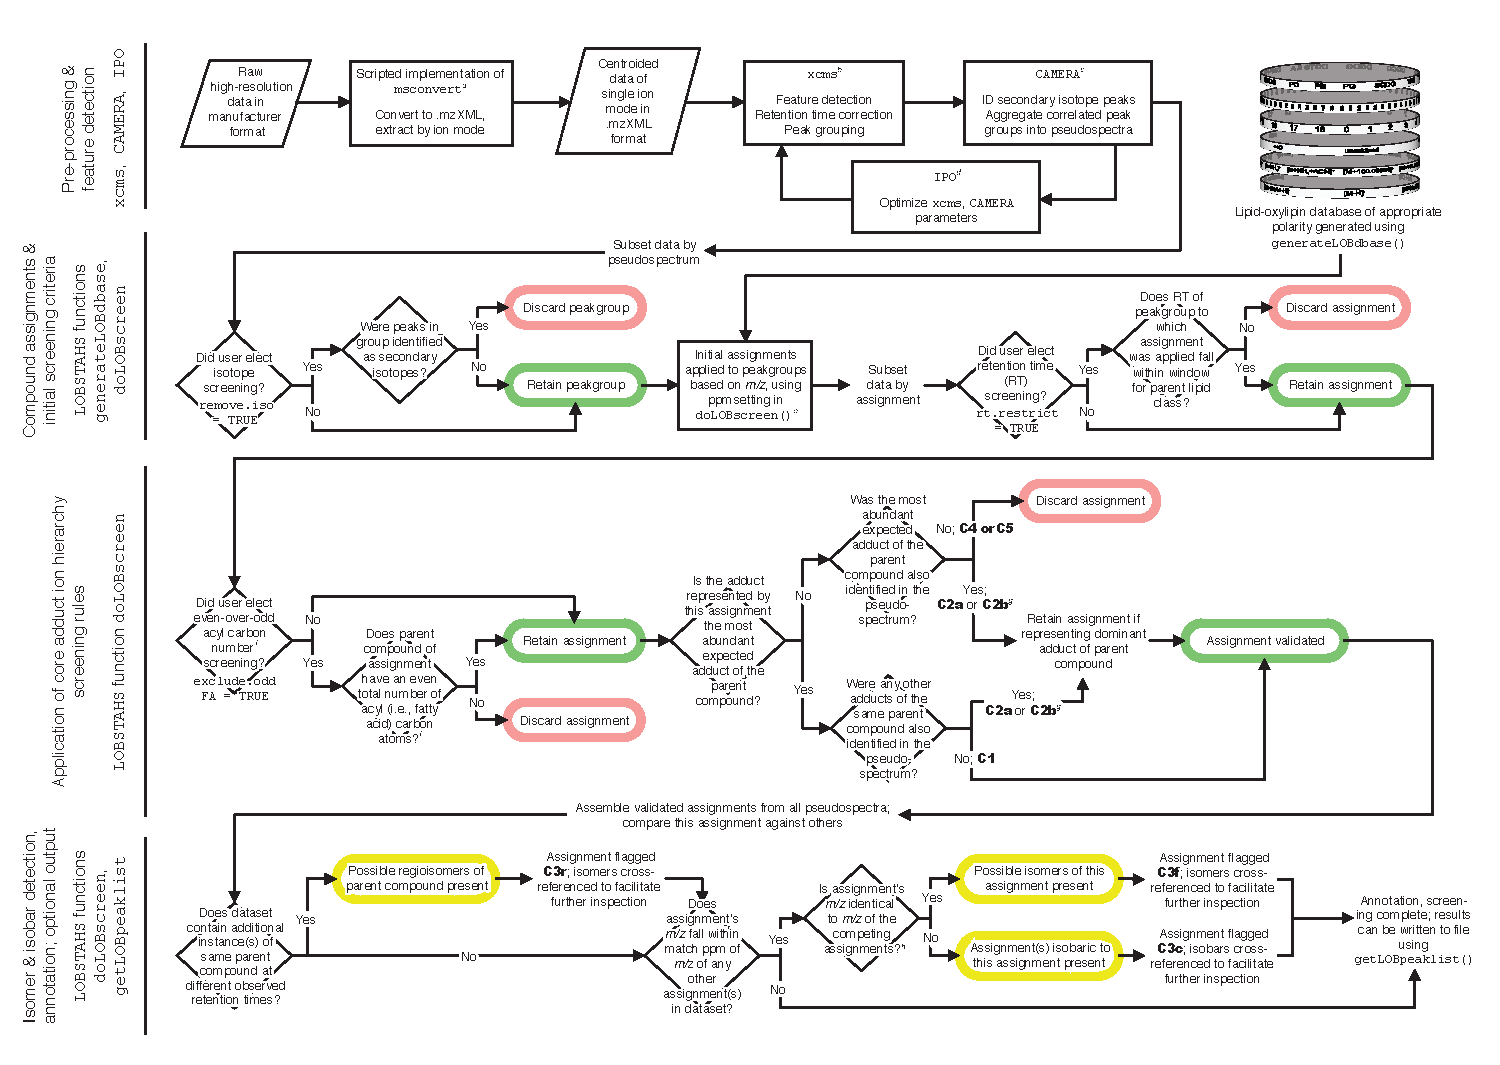
\includegraphics[width=1.05\textwidth]{Fig_3-1.pdf}
\captionsetup{font={footnotesize}}
\caption[Preparation, Screening, and Annotation of HPLC-MS Lipid Data Using LOBSTAHS]{Preparation, Screening, and Annotation of HPLC-MS Lipid Data Using LOBSTAHS. Annotation codes (in bold) may be applied as indicated; these are designed to assist the user in evaluating assignment confidence during subsequent data analysis.\\
\emph{\textsuperscript{a}} We automate several functions of the ProteoWizard msConvert tool (Kessner et al., 2008).\\
\textsuperscript{\emph{b},\emph{c}} xcms (Benton et al., 2010; Smith et al., 2006; Tautenhahn et al., 2008) was chosen for its command-line features and because it permits follow-on use of the R package CAMERA (Kuhl et al., 2012) to identify isotopes.\\
\emph{\textsuperscript{d}} IPO (Libiseller et al., 2015) can be used to optimize the values of parameters for some xcms and CAMERA functions.\\
\emph{\textsuperscript{e}} Multiple assignments will likely exist for many peakgroups in a typical dataset.\\
\emph{\textsuperscript{f}} This criterion may be useful when the subject dataset contains lipids of exclusively eukaryotic origin.\\
\emph{\textsuperscript{g}} In case C2a, the adduct ion hierarchy for the parent compound is completely satisfied; i.e., the pseudospectrum contains peakgroups representing every adduct ion of the compound of greater theoretical abundance than the least abundant adduct ion present. In case C2b, the adduct ion of greatest theoretical abundance and some lesser adduct ion is present, but adduct ions of intermediate abundance are not observed.\\
\textsuperscript{\emph{h}} Both outcomes may apply simultaneously at this decision point if the dataset contains isobars and isomers of the assignment.}
\label{fig:c3n1}
\end{figure}

Next, LOBSTAHS can screen the feature's retention time against a retention time ``window'' defined for the accompanying assignment's parent lipid class. LOBSTAHS includes a set of default retention time window data (\autoref{table:adn4}) for the chromatographic conditions we describe here. Detailed instructions for application of retention time data from other chromatographic methods are included in the Supporting Information. A third filter can then be applied to exclude assignments of IPL, ox-IPL, FFA, and PUA that contain an odd total number of acyl carbon atoms. We envision that this filter would be applied to data of exclusively eukaryotic origin: Since non-acetogenic fatty acid synthesis is confined almost exclusively to bacteria and archaea (Pearson, 2014), FA synthesized by eukaryotes will be composed of an even total number of carbon atoms.

After applying these initial optional criteria, LOBSTAHS then screens each assignment using adduct ion hierarchy data (\autoref{fig:c3n1}, ``Application of core adduct ion hierarchy screening rules''; \autoref{table:adn2}). This screening serves as the primary orthogonal filter to eliminate any confounding secondary isotopes and unassigned lipid-extractable features still remaining in the dataset. During this process, LOBSTAHS uses a series of rules to compare the relative abundance ranks of sets of adduct ion assignments that have the same parent compound. The package makes several annotations using simple codes that indicate the degree to which the assignment complies with the hierarchy rules (\autoref{fig:c3n1}, in bold). Assignments that fail the adduct ion hierarchy screening criteria are excised from the dataset and all remaining assignments in the dataset are then pooled.

Additional rules-based screening is then performed on the pooled data to identify and annotate possible isomers and isobars (\autoref{fig:c3n1}, ``Isomer \& isobar detection, annotation''). Codes can be applied to identify positional or regioisomers (code C3r), functional structural isomers (code C3f), or isobars (code C3c). LOBSTAHS can apply several of these different codes to a given assignment as long as the criterion for each is satisfied. Upon completion of screening, LOBSTAHS produces an R object containing the annotated dataset. Statistical analysis can then be performed in R on the final matrix of compound assignments, or the results can be exported to a .csv file for external analysis.

\section{Experimental Section}

\subsection{Model Dataset Used to Demonstrate the Workflow}

To demonstrate LOBSTAHS, we applied the workflow in \autoref{fig:c3n1} to examine the effect of oxidative stress on a model algal lipidome. For the analysis, we used lipid data collected from cultures of a mutant strain of the marine diatom \emph{Phaeodactylum tricornutum}, which was designed for studies of oxidative stress. In the study (van Creveld et al., 2015), a strain of \emph{P. tricornutum} (CCMP2561; Provasoli-Guillard National Center for Marine Algae and Microbiota) was genetically modified (Rosenwasser et al., 2014) to express a reduction-oxidation sensitive green fluorescent protein (roGFP) at different locations within the cell (Dooley et al., 2004; Hanson et al., 2004). Cultures of the transformants were treated with three concentrations of H\textsubscript{2}O\textsubscript{2} (0, 30, and 150 $\mu$mol L\textsuperscript{-1}) to evaluate the effects of peroxidation; culture conditions are described in van Creveld et al. (2015).

\subsection{Sample Collection and Extraction}

In the experiment, duplicate samples for lipid analysis were collected from each treatment at 4, 8, and 24 h timepoints. Two procedural blanks were also collected. Sample material was collected by vacuum onto 0.7 $\mu$m pore size glass fiber filters (GF/F), which were snap frozen in liquid nitrogen and then stored at -80$^{\circ}$C until thawed for extraction. Extraction was performed using a modified Bligh and Dyer (Bligh and Dyer, 1959) method described in Popendorf et al. (2013); an internal standard (dinitrophenyl-phosphatidylethanolamine, DNP-PE) and a synthetic antioxidant (butylated hydroxytoluene, BHT) were added at time of extraction. Lipid extracts were transferred to 2 mL HPLC vials, topped with argon, and stored at -80$^{\circ}$C prior to analysis. All chemicals used in sample extraction and chromatography were LC/MS grade or higher. Where used, water was obtained from a Milli-Q system without further treatment (EMD Millipore, Billerica, MA, USA).

\subsection{HPLC-ESI-MS Analysis}

Samples from the \emph{P. tricornutum} dataset were analyzed by HPLC-ESI-MS using a modification of the method described in Hummel et al. (2011) Lipid extracts were evaporated to near dryness and reconstituted in a similar volume of 7:3 acetonitrile:isopropanol. Headspace was filled with argon to minimize further oxidation. For HPLC analysis, an Agilent 1200 system (Agilent, Santa Clara, CA, USA) comprising temperature-controlled autosampler (4$^{\circ}$C), binary pump, and diode array detector, was coupled to a Thermo Exactive Plus Orbitrap mass spectrometer (ThermoFisher Scientific, Waltham, MA, USA). Chromatographic conditions, electrospray ionization source settings, MS acquisition settings, and procedures used for calibration of the mass spectrometer are described in the Supporting Information. Using authentic standards and two independent methods for MS feature detection, we determined the average relative mass uncertainty of the Exactive was \textless{} 0.2 ppm (\autoref{table:c3n1}; \autoref{table:adn6}); evaluation of these standards is discussed below.

\subsection{Analysis of \emph{P. tricornutum} Data Using LOBSTAHS}

xcms, CAMERA, and LOBSTAHS were then used to identify and annotate lipidome components in the positive ionization mode data. The R package IPO (Libiseller et al., 2015) was used to optimize settings for several xcms functions, and a 2.5 ppm mass uncertainty tolerance was used to obtain database matches in LOBSTAHS. Using the annotated output we obtained from LOBSTAHS, we then calculated the relative abundances of lipidome constituents present in the 0 and 150 $\mu$M H\textsubscript{2}O\textsubscript{2} treatments at 24 h. Statistical techniques were used to identify biomarkers of oxidative stress. Unless otherwise noted, we restricted our analysis to only ``high confidence'' assignments; these were assignments without structural isomers or isobars given codes of C1 or C2a according to the logic in \autoref{fig:c3n1}. The specific settings used in xcms, CAMERA, and LOBSTAHS, details of statistical methods, and links to scripts we used to obtain results and figures are included in the Supporting Information text and \autoref{table:adn5}.

\section{Results and Discussion}

\subsection{Screening and Annotation of \emph{P. tricornutum} Data in LOBSTAHS}

Using LOBSTAHS, we identified 21,869, or 6.4\%, of the 340,991 mass spectral features initially detected in the dataset using xcms. Sequential application of the various screening criteria allowed us exclude features from the dataset based on specific characteristics (\autoref{table:c3n2}). Of these initial features, 177,053, or 52\%, were immediately eliminated as likely secondary isotope peaks identified by CAMERA. The 163,938 remaining features were then matched at 2.5 ppm against entries in the default positive mode database. We then used LOBSTAHS to perform screening based on feature retention time and assignment total acyl carbon number. LOBSTAHS excluded 7,792 features because the retention time fell outside the range expected for the assignment's parent lipid class. An additional 7,733 features were eliminated because the compound assignment did not contain an even total number of acyl carbon atoms; this optional restriction was applied given the known eukaryotic origin of the data. Adduct ion hierarchy screening was then applied to the remaining 52,337 features. Application of this final orthogonal filter yielded a dataset containing 2,056 compound assignments; these assignments represented 1,969 unique parent compounds (\autoref{table:c3n2}).

\begin{SCfigure}[1][!t]
\centering
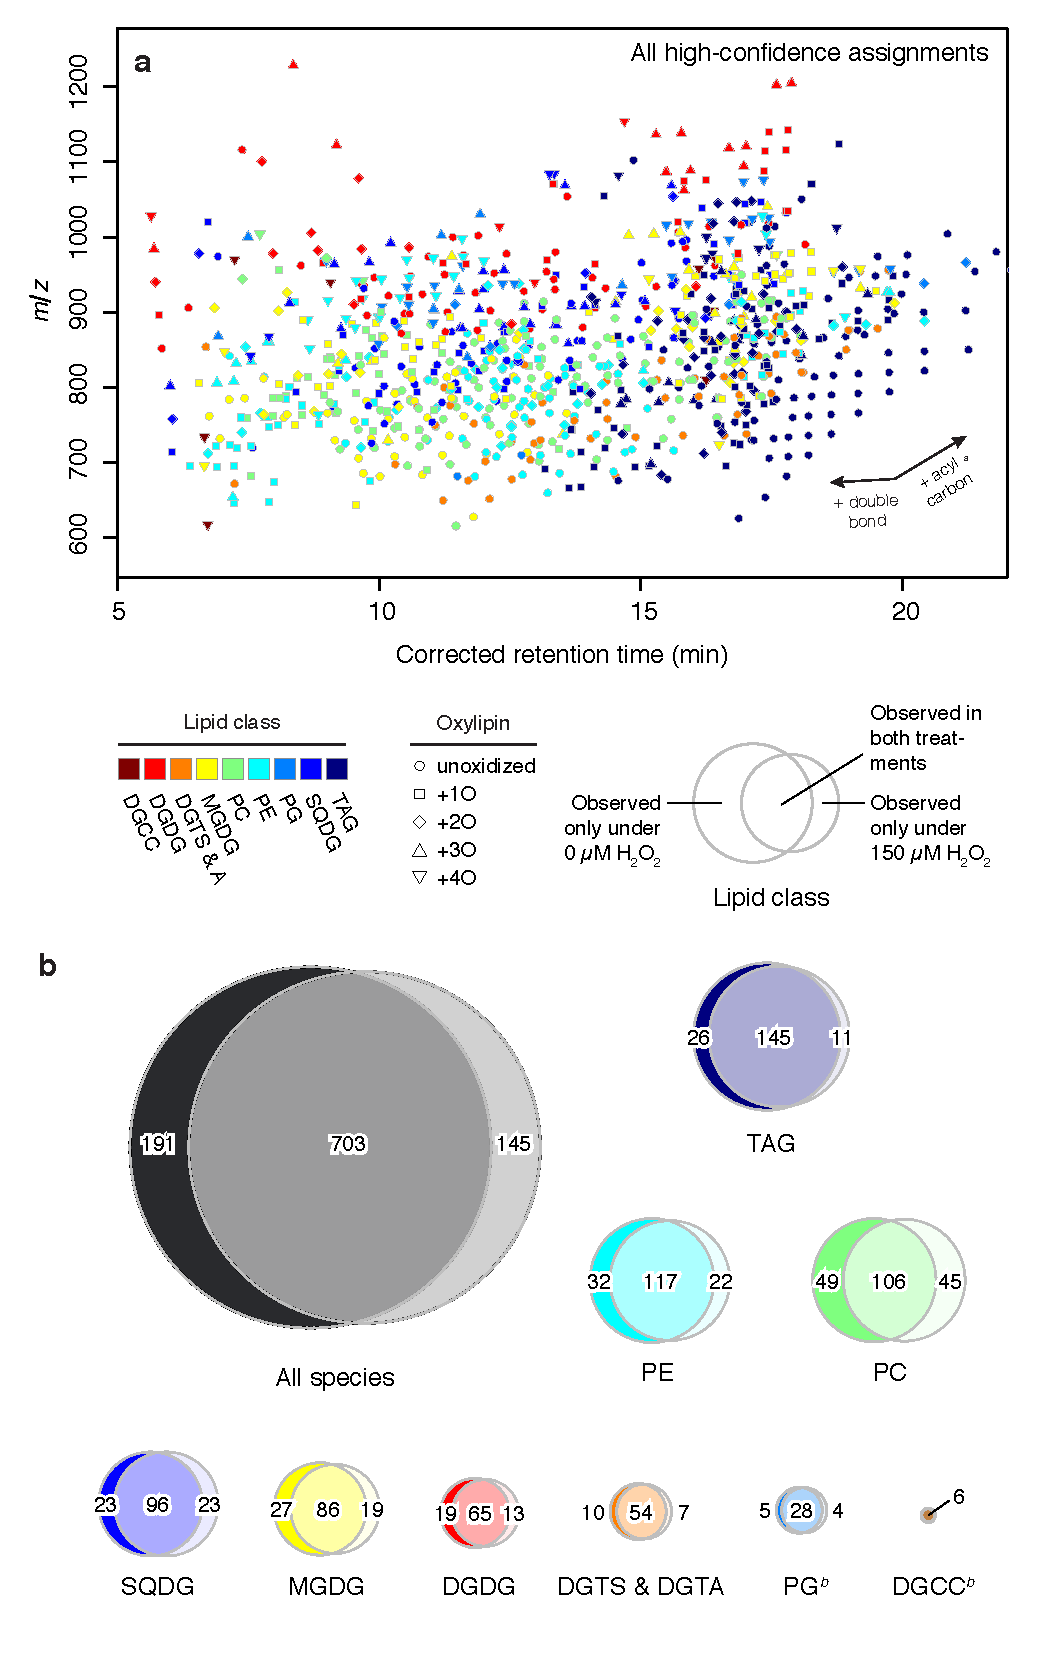
\includegraphics[width=.65\textwidth]{Fig_3-2.pdf}
\captionsetup{font={footnotesize}}
\caption[IPL, ox-IPL, and TAG identified in the \emph{P. tricornutum} dataset]{(a) All IPL, ox-IPL, and TAG identified in the \emph{P. tricornutum} dataset with high confidence (\emph{N} = 1039; figure excludes pigments). (b) Distribution by lipid class of high-confidence assignments made in the 0 and 150 $\mu$M H\textsubscript{2}O\textsubscript{2} treatments at 24 h (\emph{N} = 894 and \emph{N} = 848, respectively). Ellipse size in (b) reflects the number of compounds identified within each class and treatment. The assignments presented in (a) and (b) fully satisfied the LOBSTAHS adduct hierarchy screening criteria (i.e., annotated ``C1'' or ``C2a'' according to the logic in \autoref{fig:c3n1}) and had no competing assignments, such as possible structural isomers, identified in the dataset. Excluded are those compounds having an odd total number of acyl carbon atoms.\\
\emph{\textsuperscript{a}} General direction of movement within \emph{m/z} versus RT plot, for a given lipid class and oxidation state. The direction of movement that results from addition or removal of additional oxygen atom(s) varies by lipid class.\\
\emph{\textsuperscript{b}} Not to scale.}
\label{fig:c3n2}
\end{SCfigure}

The identities of 1,163, or 57\%, of these final database assignments were unique within the scope of our database, meaning the underlying features were matched in the final dataset to only one possible parent compound. 1,149 of these assignments were either IPL, ox-IPL, or TAG (\autoref{fig:c3n2}a); the remainder were photosynthetic pigments. We classified 1,056 of these identifications as ``high confidence,'' indicating that the distribution of adducts present in the constituent features perfectly satisfied the adduct hierarchy rules (\autoref{fig:c3n2}a and symbols with darkest tones in \autoref{fig:adn2}-\autoref{fig:adn10}); these were used in the analysis below.

\subsubsection{Identification and Annotation of Isomers and Isobars}

The remaining 893 assignments (43.4\%) were characterized by some degree of ambiguity, meaning the dataset contained at least one isobar or structural functional isomer of the underlying features (\autoref{table:adn7}; symbols with lightest tones in Figures \autoref{fig:adn2}-\autoref{fig:adn10}). In 752 instances, the dominant adduct of the parent compound was a (functional) structural isomer of the dominant adduct of a different compound assigned from the database (\autoref{table:adn9}, first example). In 195 cases, the dominant adduct ion of the parent compound was an isobar of the primary adduct ion of a different compound (\autoref{table:adn9}, second example). Although these ambiguous assignments represented 43.4\% of all assignments in the screened dataset, they belonged to just 25\% of retained features (27\% of peak groups; \autoref{table:adn7}). The difference was due to the presence of a small number of features (793) whose 54 assignments were doubly ambiguous, i.e., having both isobars and functional structural isomers (symbols with two-tone shading in \autoref{fig:adn2}-\autoref{fig:adn10}; \autoref{table:adn9}, third example). The number of competing assignments for each identified compound varied largely by lipid class. For example, LOBSTAHS found no functional structural isomers for compounds identified in several lipid classes: digalactosyldiacylglycerol (DGDG), phosphatidylethanolamine (PE), and sulfoquinovosyldiacylglycerol (SQDG) (\autoref{fig:adn3}, \autoref{fig:adn7}, and \autoref{fig:adn9}). Doubly ambiguous assignments were confined to only four classes: diacylglyceryl carboxyhydroxymethylcholine (DGCC), diacylglyceryl trimethylhomoserine and diacylglyceryl hydroxymethyl-trimethyl-$\beta$-alanine (DGTS \& DGTA), phosphatidylcholine (PC), and phosphatidylglycerol (PG) (\autoref{fig:adn2}, \autoref{fig:adn4}, \autoref{fig:adn6}, and \autoref{fig:adn8}).

\subsubsection{Annotation of Potential Regioisomers}

LOBSTAHS also identified regioisomers for 352 unique parent compounds in the \emph{P. tricornutum} lipidome (\autoref{table:adn7}; symbols with black dots in \autoref{fig:adn2}-\autoref{fig:adn10}). These were instances in which the same assignment was applied to two or more features appearing at different retention times in the same sample. Many of these assignments were oxylipins and ox-IPL, indicating the presence of multiple oxidized isomers of the same parent IPL that could be used as biomarkers for oxidative stress. Without further analysis, we were unable to determine whether these isomers represented the oxidation of a fatty acid by the same mechanism at a different acyl carbon position, or instead the presence of different oxidized functional groups that yielded equivalent exact masses (e.g., a dihydroxy-, hydroperoxy-, or $\alpha$- or $\gamma$-ketol acid). The level of identification and annotation provided by LOBSTAHS supports a wide range of possible molecular structures for each assignment; an example from the dataset is presented in \autoref{table:adn9}. The data were consistent with studies in both model plant (Buseman et al., 2006; Vu et al., 2012) and animal (Ni et al., 2015) systems that demonstrated the coexistence of a diversity of ox-IPL with both their parent IPL and smaller, traditional oxylipin degradation products.

\subsection{Evaluation of Screening and Identification Performance using Two Methods}

As a means of validating the accuracy and reliability of our approach, we asked LOBSTAHS to identify and annotate all species present in 5 quality control (QC) samples of known composition that were interspersed randomly with samples from the \emph{P. tricornutum} dataset prior to analysis on the mass spectrometer (\autoref{table:c3n1}; \autoref{table:adn6}). The samples contained a mixture of authentic IPL standards that has been used extensively in other work in our laboratory (Popendorf et al., 2013; Van Mooy and Fredricks, 2010). Because the choice of pre-processing software can have a significant impact on feature detection (Cajka and Fiehn, 2016), we conducted parallel analyses with both xcms/CAMERA and an alternative program, MAVEN (Clasquin et al., 2012; Melamud et al., 2010). In both cases, LOBSTAHS correctly identified all components of the standard mixture without ambiguity (\autoref{table:c3n1}; \autoref{table:adn6}). Because purified standards do not exist for long-chain ox-IPL, we were unable to directly evaluate the Type 1 error rate for their identification. As a second means of validation, we compared assignments in the screened dataset to two independent inventories of the \emph{P. tricornutum} lipidome (Abida et al., 2015; Levitan et al., 2015). LOBSTAHS found and identified with high confidence 13 of the 16 most abundant IPL and TAG species in one inventory (Abida et al., 2015), and nearly all those in the other (Levitan et al., 2015). While our approach also correctly identified the three remaining components in the former study (PG 32:1, PG 36, and DGTS \& DGTA 40:10), functional structural isomers or isobars made unambiguous identification impossible without further manual inspection of MS\textsuperscript{2} spectra.

\subsection{Resilience of Core \emph{P. tricornutum} Lipidome under Oxidative Stress}

Evidence of the effect of oxidative stress on the lipidome of \emph{P. tricornutum} was observed through comparison of compounds identified in 0 and 150 $\mu$M H\textsubscript{2}O\textsubscript{2} treatments at 24 h (\autoref{fig:c3n2}, \autoref{fig:c3n3}a,b, and \autoref{table:adn9}). That the two treatments produced only subtle differences in molecular diversity (\autoref{fig:c3n2}b) suggests much of the core lipid inventory remained robust to the imposed oxidative stress. The vast majority of the 949 oxidized and unoxidized lipid moieties we identified in the healthy organism (879, or 92.6\%) could still be identified in the lipidome of the stressed cultures (\autoref{fig:c3n2}b). On the basis of peak area, oxidized lipid moieties accounted for 5-7\% of the \emph{P. tricornutum} lipidome across nearly all treatments and timepoints. Based on the relatively consistent size of this oxidized lipid fraction and its persistence in even the 0 $\mu$M H\textsubscript{2}O\textsubscript{2} treatment, we consider it a quantitative constraint on the baseline level of lipid peroxidation associated with metabolic processes in photosynthetic organisms (Apel and Hirt, 2004; Crastes de Paulet et al., 1988).

\begin{SCfigure}[1][!t]
\centering
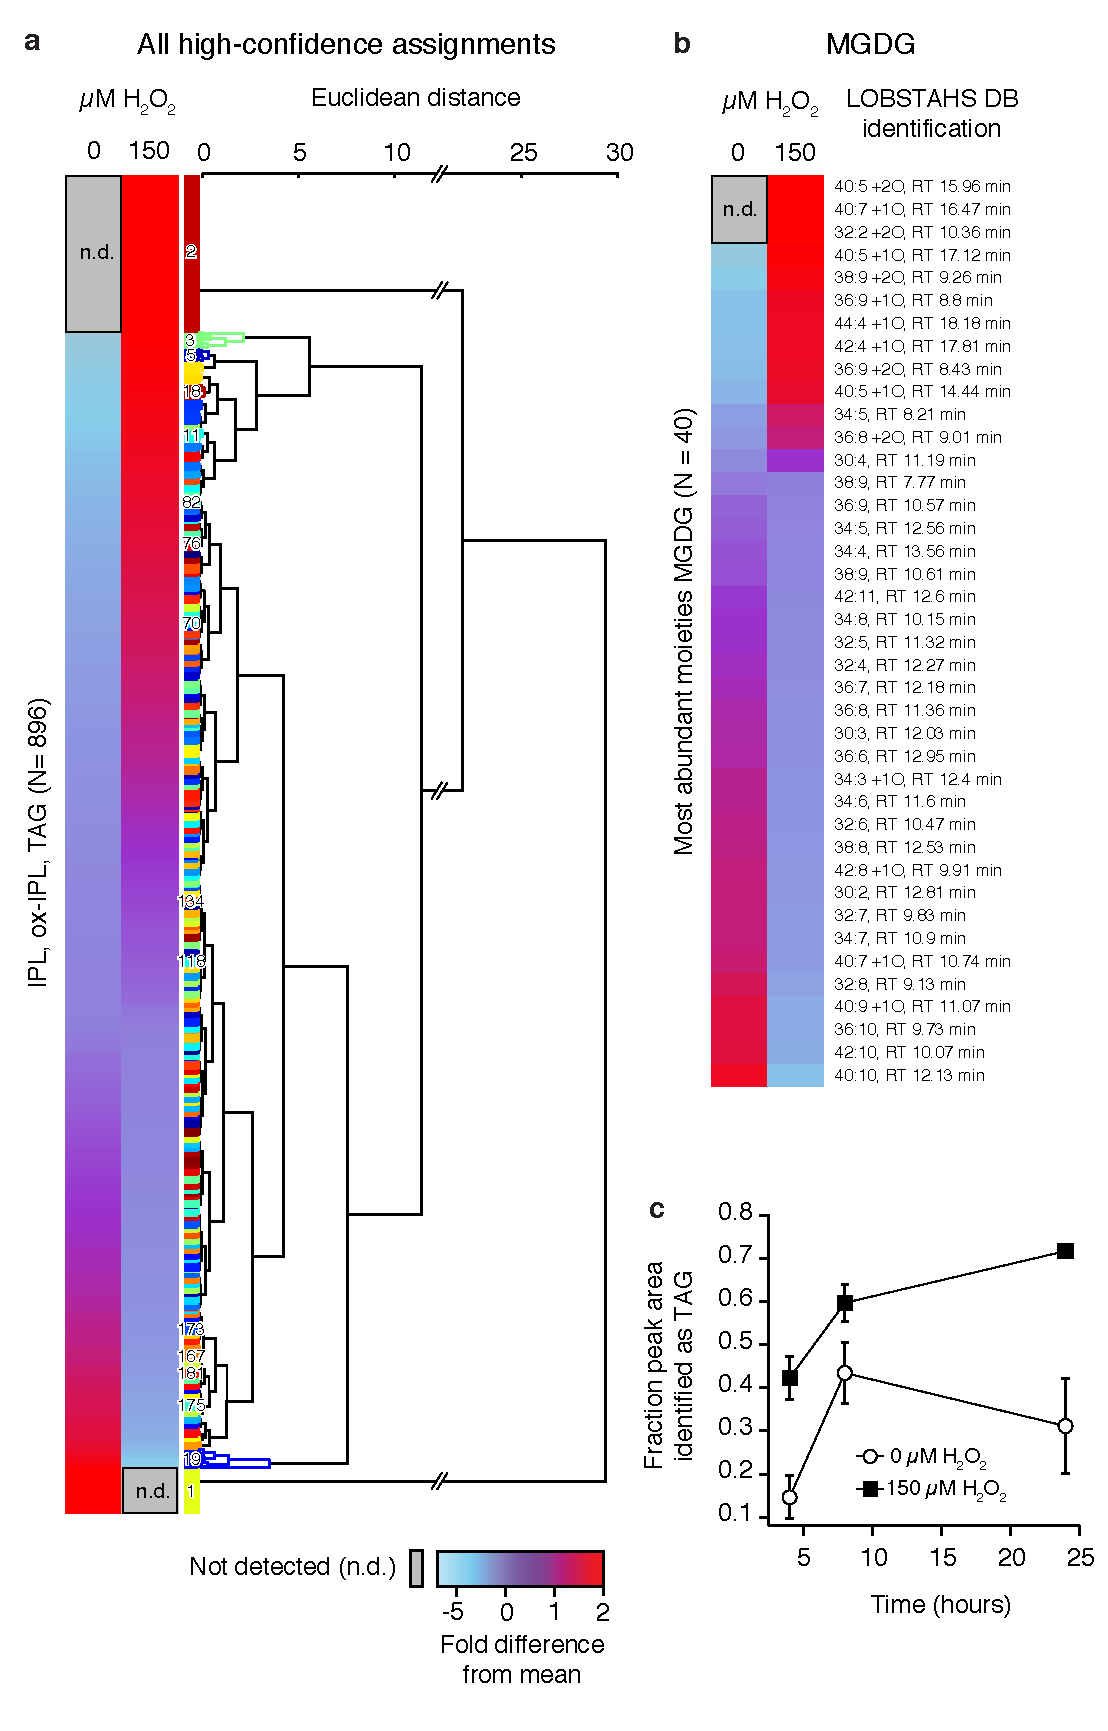
\includegraphics[width=.55\textwidth]{Fig_3-3.pdf}
\captionsetup{font={footnotesize}}
\caption[Remodeling of the \emph{Phaeodactylum tricornutum} lipidome after 24 h, as visualized from data analyzed with LOBSTAHS]{Remodeling of the \emph{Phaeodactylum tricornutum} lipidome after 24 h, as visualized from data analyzed with LOBSTAHS. (a) Heatmap showing relative abundances across two treatments (0 and 150 $\mu$M H\textsubscript{2}O\textsubscript{2}) of all IPL, ox-IPL, and TAG identified with high confidence. Each row (\emph{N} = 896) represents a different compound identified from the database; \autoref{fig:adn11} contains an expanded version of the plot that includes labels for each individual compound. (b) Heatmap detail, showing changes in the most abundant (\emph{N} = 40) moieties of monogalactosyldiacylglycerol (MGDG), a lipid typically localized to the chloroplast. (c) Fraction of total peak area identified as triacylglycerol (TAG) at three timepoints during the experiment. Error bars are $\pm$ SD of two replicates. In (a) and (b), shading shows the relative abundance of each compound as a fold difference of the mean peak area observed in that treatment from the mean peak area of the compound observed across all treatments. Dendrogram clustering and group definitions were determined by similarity profile analysis (Clarke et al., 2008). The numbers and identities of the components assigned to each group in (a) are given in \autoref{table:adn5} and \autoref{fig:adn11}. Solid black lines in the dendrogram indicate branching that was statistically significant (\emph{p} $\leq$ 0.01).}
\label{fig:c3n3}
\end{SCfigure}

\subsection{Differences in Degree of Remodeling Between Lipid Classes and Functional Groupings}

We used similarity profile analysis of the scaled LOBSTAHS data (Clarke et al., 2008) to place the annotated features into 181 groups of components which clustered significantly according to their behavior (\autoref{fig:c3n3} and \autoref{fig:adn1}1). The components of each group are given in \autoref{table:adn8}. We further examined the up- and downregulation of lipidome components under oxidative stress by dividing potential biomarkers into classes based on their molecular headgroups (\autoref{table:adn9}). This allowed us to examine class-specific differences in the number of acyl carbon atoms, acyl carbon-to-carbon double bonds, and oxidation states (i.e., additional oxygen atoms) of component lipids under the two treatments. Differential expression of chemical properties within several classes (\autoref{fig:c3n3}; \autoref{table:adn9}) suggested the \emph{P. tricornutum} lipidome was remodeled in subtle but pervasive ways.

\subsection{Fatty Acid Chain Elongation is an Apparent Response to Oxidative Stress in the Chloroplast}

Oxidative stress appeared to induce elongation of fatty acids throughout the \emph{P. tricornutum} lipidome (\autoref{table:adn9}). Lipid moieties upregulated by oxidative stress had longer fatty acid chains than those that were downregulated. We observed the greatest breadth of structural change in monogalactosyldiacylglycerol (MGDG), a lipid typically localized to the chloroplast (\autoref{table:adn9}; \autoref{fig:c3n3}b). Moieties of MGDG upregulated in the 150 $\mu$M H\textsubscript{2}O\textsubscript{2} treatment had significantly longer fatty acid chains and were more oxidized than those downregulated under oxidative stress; oxidation and elongation were also accompanied by a statistically significant decrease in acyl chain unsaturation (\autoref{table:adn9}). The MGDG moieties responsible for these shifts in class structural properties were confined largely to groups 1, 2, 4, 5, 7, 9, 12, 166, 167, and 180 in our similarity profile analysis (\autoref{fig:c3n3}b and \autoref{fig:adn11}; \autoref{table:adn8}). Lipid oxidation has been previously linked in the diatom \emph{Skeletonema costatum} to lipolytic cleavage of MGDG and phospholipids within the chloroplast, resulting in oxylipin production from free fatty acids (d'Ippolito et al., 2004). While intact oxidized MGDG species have not been previously observed in algae, ox-MGDG have been documented in terrestrial plants upon wounding (Vu et al., 2012). The production of ox-IPL in \emph{Arabidopsis thaliana} may be a means of binding ROS within the cell membrane to limit damage elsewhere (M\`{e}ne-Saffran\'{e} et al., 2009).

\subsection{Fatty Acid Chain Elongation Also Evident in Lipids Localized to Other Cell Compartments}

In addition to observations of fatty acid chain elongation in lipids typical of the chloroplast, significant elongation was also observed in moieties of phosphatidylethanolamine (PE) that were upregulated upon treatment with 150 $\mu$M H\textsubscript{2}O\textsubscript{2}. When lipids typical of the chloroplast (DGDG, SQDG, MGDG, and PG), endoplasmic reticulum (PC, PG, PE), and mitochondrion (PE and PG) were considered separately (Jouhet et al., 2010), we found that lipids with longer chain fatty acids were upregulated in mitochondria but not in the endoplasmic reticulum (\autoref{table:adn9}). While our analysis suggested that oxidative stress in \emph{P. tricornutum} resulted in a global shift toward lipids with longer chain fatty acids, the opposite lipidomic response was observed for \emph{P. tricornutum} under nitrogen stress (Yang et al., 2013). Nitrogen stress resulted in a decrease in both eicosapentaenoic (EPA; 20:5) and docosahexaenoic (DHA; 22:6) acids and a shift toward shorter chain length palmitic (16:0) and palmitoleic (16:1) acids (Yang et al., 2013). We do not view the data we obtained using LOBSTAHS as incompatible with these findings; instead, the result suggests that different sources of stress upon the cell can induce specific and distinct signatures in the lipidome of \emph{P. tricornutum}.

\subsection{Significant Enrichment Observed in TAG}

Whereas the impact of oxidative stress within most lipid classes was confined to relatively modest changes in structural properties, treatment with 150 $\mu$M H\textsubscript{2}O\textsubscript{2} induced a very significant enrichment in the fraction of peak area we identified as triacylglycerols (TAG; \autoref{fig:c3n3}c). Enigmatically, the TAG moieties upregulated in the 150 $\mu$M treatment were significantly less oxidized than those downregulated (\autoref{table:adn9}). We hypothesize that the growth of this chemically reduced TAG pool may be evidence of enhanced \emph{de novo} production of un-oxidized TAG as a response to oxidative stress. Increased TAG synthesis is a known response to nutrient starvation in virtually all algae (Goncalves et al., 2016; Merchant et al., 2012), including in \emph{P. tricornutum} (Abida et al., 2015; Levitan et al., 2015). While increased TAG production in algae has not been previously linked directly to oxidative stress, increased production has been observed as a response to viral infection in the haptophyte alga \emph{Emiliania huxleyi} (Hunter et al., 2015).

\subsection{No Overall Increase Observed in Lipidome Oxidation State}

Enigmatically, we found no statistically significant differences in either the peak area allocated to oxidized lipid moieties or in the fraction of unique compounds identified as oxidized (\autoref{table:adn9}; calculations not shown). One explanation for this finding is that the cultures were not sampled soon enough after treatment with H\textsubscript{2}O\textsubscript{2} to observe oxidation of the lipidome before a rapid antioxidant response was induced in the organism. By 4 hours, the first timepoint at which the experiment was sampled, it is not unreasonable to expect that repair of much of the initial oxidative damage would already have been underway via upregulation of a suite of enzymatic and non-enzymatic plant antioxidant defense mechanisms (Lesser, 2006; Gill and Tuteja, 2010). In \emph{Arabidopsis thaliana}, the lipidomic response to wounding, another source of oxidative stress, was nearly instantaneous; concentrations of several intact oxidized lipid species increased by as much three orders of magnitude within 15 minutes after the treatment was applied (Buseman et al., 2006).

\section{Conclusion}

Using a model dataset, LOBSTAHS allowed us to identify differences in lipid speciation between treatments that could be used as potential indicators oxidative stress in \emph{P. tricornutum}. This potential extended beyond individual oxylipins and ox-IPL to sets of highly interrelated compounds that represented different stages of degradation and oxidation within the same lipidome (\autoref{fig:c3n3} and \autoref{fig:adn11}; \autoref{table:adn8}). While we demonstrated our approach using culture data from a single marine diatom, we designed LOBSTAHS so it can be used with exact-mass HPLC/MS data from virtually any experiment or natural system.

For a minority of features in the screened dataset that had isobars and/or structural isomers (\autoref{table:adn7}; \autoref{fig:adn2}-\autoref{fig:adn10}), we were unable to make unambiguous identifications using LOBSTAHS alone. Many of these could be identified more rigorously through comparison with results from alternative commercial software or by manual inspection using authentic standards or diagnostic MS fragmentation patterns. Our objective, however, was not to definitively characterize a few individual compounds with absolute certainty, but instead to putatively identify a broad range of possible biomarkers for further analysis and discovery with a level of certainty between Level 3 (``Putatively characterized compound classes'') and Level 2 (``Putatively annotated compounds''), using the scheme of Sumner et al. (2007), The overall results we obtained with the \emph{P. tricornutum} dataset demonstrate the ability of LOBSTAHS to assist in this task. The screening and annotation process allowed us to assess a range of levels of confidence on the putative assignments, producing an ample subset of high-confidence compound identifications sufficient to facilitate a detailed statistical analysis. Future integration of methods such as chiral HPLC (Senger et al., 2005) or matching of diagnostic MS\textsuperscript{2} fragmentation spectra, with screening tools such as the one we present here will assist in discovery of biomarkers in larger datasets and with even greater confidence.

\section{Acknowledgments }

We thank Elizabeth Kujawinski, Winn Johnson, and Krista Longnecker for discussions on the analysis of metabolomics datasets and assistance with xcms; Marian Carlson and Matthew Johnson for discussions on the effects of oxidative stress in microorganisms; Assaf Vardi and Daniella Schatz for providing the \emph{P. tricornutum} cell cultures; and Eugene Melamud for answering our many questions about MAVEN. Liz Kujawinski provided thoughtful feedback on an earlier version of the manuscript. Finally, we thank two anonymous reviewers for critical comments that improved the manuscript significantly. This research was supported by the Gordon and Betty Moore Foundation through Grant GBMF3301 to B.A.S.V.M. This research was also funded in part by a grant to B.A.S.V.M. from the Simons Foundation and is a contribution of the Simons Collaboration on Ocean Processes and Ecology (SCOPE). J.R.C. acknowledges support from a U.S. Environmental Protection Agency (EPA) STAR Graduate Fellowship (Fellowship Assistance Agreement no. FP-91744301-0).

\section{Availability of Data and Code }

The current release of the LOBSTAHS package can be compiled using R devtools from source files maintained at \url{https://github.com/vanmooylipidomics/LOBSTAHS}. A readme file and R vignette in the repository contain step-by-step installation and operation instructions. The fully processed \emph{Phaeodactylum tricornutum} dataset is available from \url{https://github.com/vanmooylipidomics/PtH2O2lipids} as the R data package PtH2O2lipids. Both packages are provided under the MIT License. Auxiliary R scripts necessary for pre-processing of data are maintained at \url{https://github.com/vanmooylipidomics/LipidomicsToolbox}. Raw files for the \emph{P. tricornutum} dataset may be downloaded at \url{ftp://ftp.whoi.edu/pub/science/MCG/gbmf/VanMooy/OxylipinAnalysis}; metadata for the dataset are provided at \url{http://www.whoi.edu/page.do?pid=133616\&tid=282\&cid=192529/}. Scripts used for statistical analysis of the \emph{P. tricornutum} dataset and to produce the figures presented in the text are available from \url{https://github.com/jamesrco/LipidomicsDataViz}. See also \autoref{sec:Supplementary Methodological Details Not Described in the Text}.

\clearpage
\begin{singlespace}
\section*{References}
\addtocounter{section}{1}
{\setlength{\parindent}{0pt}
Abida, H., L. J. Dolch, C. Mei, V. Villanova, M. Conte, M. A. Block, G. Finazzi, O. Bastien, L. Tirichine, C. Bowler, F. Rebeille, D. Petroutsos, J. Jouhet and E. Marechal (2015), Membrane glycerolipid remodeling triggered by nitrogen and phosphorus starvation in \emph{Phaeodactylum tricornutum}, \emph{Plant Physiology}, 167(1), 118-36, doi:\href{http://dx.doi.org/10.1104/pp.114.252395}{10.1104/pp.114.252395}.

{\setlength{\parskip}{10pt}

Andreou, A., F. Brodhun and I. Feussner (2009), Biosynthesis of oxylipins in non-mammals, \emph{Progress in Lipid Research}, 48(3-4), 148-170, doi:\href{http://dx.doi.org/10.1016/J.Plipres.2009.02.002}{10.1016/J.Plipres.2009.02.002}.

Andreou, A. and I. Feussner (2009), Lipoxygenases: Structure and reaction mechanism, \emph{Phytochemistry} 70(13-14), 1504-1510, doi:\href{http://dx.doi.org/10.1016/J.Phytochem.2009.05.008}{10.1016/J.Phytochem.2009.05.008}.

Apel, K. and H. Hirt (2004), Reactive oxygen species: Metabolism, oxidative stress, and signal transduction, \emph{Annual Review of Plant Biology}, 55(1), 373-399, doi:\href{http://dx.doi.org/10.1146/annurev.arplant.55.031903.141701}{10.1146/annurev.arpla\\nt.55.031903.141701}.

Balestra, C., L. Alonso-Saez, J. M. Gasol and R. Casotti (2011), Group-specific effects on coastal bacterioplankton of polyunsaturated aldehydes produced by diatoms, \emph{Aquatic Microbial Ecology}, 63(2), 123-131, doi:\href{http://dx.doi.org/10.3354/Ame01486}{10.3354/Ame01486}.

Balvers, M. G., K. C. Verhoeckx, S. Bijlsma, C. M. Rubingh, J. Meijerink, H. M. Wortelboer and R. F. Witkamp (2012), Fish oil and inflammatory status alter the n-3 to n-6 balance of the endocannabinoid and oxylipin metabolomes in mouse plasma and tissues, \emph{Metabolomics} 8(6), 1130-1147, doi:\href{http://dx.doi.org/10.1007/s11306-012-0421-9}{10.1007/s11306-012-0421-9}.

Benton, H. P., E. J. Want and T. M. D. Ebbels (2010), Correction of mass calibration gaps in liquid chromatography-mass spectrometry metabolomics data, \emph{Bioinformatics}, 26(19), 2488-2489.

Bligh, E. G. and W. J. Dyer (1959), A rapid method of total lipid extraction and purification, \emph{Canadian Journal of Biochemistry and Physiology}, 37, 911-917.

Br\"{u}gger, B. (2014), Lipidomics: analysis of the lipid composition of cells and subcellular organelles by electrospray ionization mass spectrometry, \emph{Annual Review of Biochemistry}, 83(1), 79-98, doi:\href{http://dx.doi.org/10.1146/annurev-biochem-060713-035324}{10.1146/annurev-biochem-060713-035324}.

Bruins, M. J., A. D. Dane, K. Strassburg, R. J. Vreeken, J. W. Newman, N. Salem, Jr., C. Tyburczy and J. T. Brenna (2013), Plasma oxylipin profiling identifies polyunsaturated vicinal diols as responsive to arachidonic acid and docosahexaenoic acid intake in growing piglets, \emph{Journal of Lipid Research}, 54(6), 1598-607, doi:\href{http://dx.doi.org/10.1194/jlr.M034918}{10.1194/jlr.M034918}.

Buseman, C. M., P. Tamura, A. A. Sparks, E. J. Baughman, S. Maatta, J. Zhao, M. R. Roth, S. W. Esch, J. Shah, T. D. Williams and R. Welti (2006), Wounding stimulates the accumulation of glycerolipids containing oxophytodienoic acid and dinor-oxophytodienoic acid in Arabidopsis leaves, \emph{Plant Physiology}, 142(1), 28-39, doi:\href{http://dx.doi.org/10.1104/pp.106.082115}{10.1104/pp.106.082115}.

Cajka, T., and O. Fiehn (2016), Toward merging untargeted and targeted methods in mass spectrometry-based metabolomics and lipidomics, \emph{Analytical Chemistry}, 88(1), 524-545, doi:\href{http://dx.doi.org/10.1021/acs.analchem.5b04491}{10.1021/acs.analchem.5b04491}.

Carini, P., B. A. S. Van Mooy, J. C. Thrash, A. White, Y. Zhao, E. O. Campbell, H. F. Fredricks and S. J. Giovannoni (2015), SAR11 lipid renovation in response to phosphate starvation, \emph{Proceedings of the National Academy of Sciences of the United States of America}, 112(25), 7767-7772, doi:\href{http://dx.doi.org/10.1073/pnas.1505034112}{10.1073/pnas.1505034112}.

Casotti, R., S. Mazza, C. Brunet, V. Vantrepotte, A. Ianora and A. Miralto (2005), Growth inhibition and toxicity of the diatom aldehyde 2-trans, 4-trans-decadienal on \emph{Thalassiosira weissflogii} (bacillariophyceae), \emph{Journal of Phycology}, 41(1), 7-20, doi:\href{http://dx.doi.org/10.1111/j.1529-8817.2005.04052.x}{10.1111/j.1529-8817.20\\05.04052.x}.

Clarke, K. R., P. J. Somerfield and R. N. Gorley (2008), Testing of null hypotheses in exploratory community analyses: similarity profiles and biota-environment linkage, \emph{Journal of Experimental Marine Biology and Ecology}, 366(1--2), 56-69, doi:\href{http://dx.doi.org/10.1016/j.jembe.2008.07.009}{10.1016/j.jembe.2008.07.009}.

Clasquin, M. F., E. Melamud and J. D. Rabinowitz (2012), LC-MS data processing with MAVEN: a metabolomic analysis and visualization engine, \emph{Current Protocols in Bioinformatics}, 37, 14.11:14.11.1--14.11.23, doi:\href{http://dx.doi.org/10.1002/0471250953.bi1411s37}{10.1002/0471250953.bi1411s37}.

Crastes de Paulet, A., L. Douste-Blazy and R. Paoletti, eds. (1988), \emph{Free Radicals, Lipoproteins, and Membrane Lipids}, Plenum Publishing Corporation, New York.

d'Ippolito, G., S. Tucci, A. Cutignano, G. Romano, G. Cimino, A. Miralto and A. Fontana (2004), The role of complex lipids in the synthesis of bioactive aldehydes of the marine diatom \emph{Skeletonema costatum}, \emph{Biochimica et Biophysica Acta}, 1686(1-2), 100-107, doi:\href{http://dx.doi.org/10.1016/J.Bblalip.2004.09.002}{10.1016/J.Bbl\\alip.2004.09.002}.

Dooley, C. T., T. M. Dore, G. T. Hanson, W. C. Jackson, S. J. Remington and R. Y. Tsien (2004), Imaging dynamic redox changes in mammalian cells with green fluorescent protein indicators, \emph{Journal of Biological Chemistry}, 279(21), 22284-93, doi:\href{http://dx.doi.org/10.1074/jbc.M312847200}{10.1074/jbc.M312847200}.

Edwards, B. R., K. D. Bidle and B. A. S. Van Mooy (2015), Dose-dependent regulation of microbial activity on sinking particles by polyunsaturated aldehydes: Implications for the carbon cycle, \emph{Proceedings of the National Academy of Sciences of the United States of America}, 112(19), 5909-5914, doi:\href{http://dx.doi.org/10.1073/pnas.1422664112}{10.1073/pnas.1422664112}.

Ejsing, C. S., E. Duchoslav, J. Sampaio, K. Simons, R. Bonner, C. Thiele, K. Ekroos and A. Shevchenko (2006), Automated identification and quantification of glycerophospholipid molecular species by multiple precursor ion scanning, \emph{Analytical Chemistry}, 78(17), 6202-14, doi:\href{http://dx.doi.org/10.1021/ac060545x}{10.1021/ac060545x}.

Fulton, J. M., H. F. Fredricks, K. D. Bidle, A. Vardi, B. J. Kendrick, G. R. DiTullio and B. A. S. Van Mooy (2014), Novel molecular determinants of viral susceptibility and resistance in the lipidome of \emph{Emiliania huxleyi}, \emph{Environmental Microbiology}, 16(4), 1137-1149, doi:\href{http://dx.doi.org/10.1111/1462-2920.12358}{10.1111/1462-2920.12358}.

Gill, S. S., and N. Tuteja (2010), Reactive oxygen species and antioxidant machinery in abiotic stress tolerance in crop plants, \emph{Plant Physiology and Biochemistry}, 48, 909-930.

Girotti, A. W. (1998), Lipid hydroperoxide generation, turnover, and effector action in biological systems, \emph{Journal of Lipid Research}, 39(8), 1529-1542.

Goncalves, E. C., A. C. Wilkie, M. Kirst and B. Rathinasabapathi (2016), Metabolic regulation of triacylglycerol accumulation in the green algae: identification of potential targets for engineering to improve oil yield, \emph{Plant Biotechnology Journal}, 14(8), 1649-60, doi:\href{http://dx.doi.org/10.1111/pbi.12523}{10.1111/pbi.12523}.

Haller, E., G. St\"{u}biger, D. Lafitte, W. Lindner and M. L\"{a}mmerhofer (2014), Chemical recognition of oxidation-specific epitopes in low-density lipoproteins by a nanoparticle based concept for trapping, enrichment, and liquid chromatography-tandem mass spectrometry analysis of oxidative stress biomarkers, \emph{Analytical Chemistry}, 86(19), 9954-9961, doi:\href{http://dx.doi.org/10.1021/ac502855n}{10.1021/ac50\\2855n}.

Hanson, G. T., R. Aggeler, D. Oglesbee, M. Cannon, R. A. Capaldi, R. Y. Tsien and S. J. Remington (2004), Investigating mitochondrial redox potential with redox-sensitive green fluorescent protein indicators, \emph{Journal of Biological Chemistry}, 279(13), 13044-53, doi:\href{http://dx.doi.org/10.1074/jbc.M312846200}{10.1074/jbc.M312846200}.

Hol\v{c}apek, M. (2015), Lipidomics, \emph{Analytical and Bioanalytical Chemistry}, 407(17), 4971-4972, doi:\href{http://dx.doi.org/10.1007/s00216-015-8740-0}{10.1007/s00216-015-8740-0}.

Hummel, J., S. Segu, Y. Li, S. Irgang, J. Jueppner and P. Giavalisco (2011), Ultra performance liquid chromatography and high resolution mass spectrometry for the analysis of plant lipids, \emph{Frontiers in Plant Science}, 2, 54, doi:\href{http://dx.doi.org/10.3389/Fpls.2011.00054}{10.3389/Fpls.2011.00054}.

Hunter, J. E., M. J. Frada, H. F. Fredricks, A. Vardi and B. A. S. Van Mooy (2015), Targeted and untargeted lipidomics of \emph{Emiliania huxleyi} viral infection and life cycle phases highlights molecular biomarkers of infection, susceptibility, and ploidy, \emph{Frontiers in Marine Science}, 2, 81, doi:\href{http://dx.doi.org/10.3389/fmars.2015.00081}{10.3389/fmars.2015.00081}.

Husen, P., K. Tarasov, M. Katafiasz, E. Sokol, J. Vogt, J. Baumgart, R. Nitsch, K. Ekroos and C. S. Ejsing (2013), Analysis of lipid experiments (ALEX): a software framework for analysis of high-resolution shotgun lipidomics data, \emph{PLoS One}, 8(11), e79736, doi:\href{http://dx.doi.org/10.1371/journal.pone.0079736}{10.1371/jo\\urnal.pone.0079736}.

Ianora, A. and A. Miralto (2010), Toxigenic effects of diatoms on grazers, phytoplankton and other microbes: a review, \emph{Ecotoxicology}, 19(3), 493-511, doi:\href{http://dx.doi.org/10.1007/S10646-009-0434-Y}{10.1007/S10646-009-0434-Y}.

Kessner, D., M. Chambers, R. Burke, D. Agus, and P. Mallick (2008), ProteoWizard: open source software for rapid proteomics tools development, \emph{Bioinformatics}, 24, 2534-2536.

Kind, T. and O. Fiehn (2006), Metabolomic database annotations via query of elemental compositions: mass accuracy is insufficient even at less than 1 ppm, \emph{BMC Bioinformatics}, 7, 234, doi:\href{http://dx.doi.org/10.1186/1471-2105-7-234}{10.1186/1471-2105-7-234}.

Kuhl, C., R. Tautenhahn, C. Bottcher, T. R. Larson and S. Neumann (2012), CAMERA: an integrated strategy for compound spectra extraction and annotation of liquid chromatography/mass spectrometry data sets, \emph{Analytical Chemistry}, 84(1), 283-9, doi:\href{http://dx.doi.org/10.1021/ac202450g}{10.1021/ac202450g}.

Kuhn, H. and S. Borngraber (1999), Mammalian 15-lipoxygenases: Enzymatic properties and biological implications, in \emph{Lipoxygenases and Their Metabolites}, edited by S. Nigam and C. R. Pace-Asciak, pp. 5-28, Plenum Publishers, New York.

Jouhet, J., E. Dubots, E. Mar\'{e}chal, and M. Block (2010), Lipid trafficking in plant photosynthetic cells, in \emph{Lipids in Photosynthesis}, edited by H. Wada and N. Murata, pp. 349-372, Springer Netherlands, Dordrecht, The Netherlands.

Lamari, N., M. V. Ruggiero, G. d'Ippolito, W. H. C. F. Kooistra, A. Fontana and M. Montresor (2013), Specificity of lipoxygenase pathways supports species delineation in the marine diatom genus \emph{Pseudo-nitzschia}, \emph{PLoS One,} 8(8), e73281, doi:\href{http://dx.doi.org/10.1371/journal.pone.0073281}{10.1371/journal.pone.0073281}.

Layre, E., L. Sweet, S. Hong, C. A. Madigan, D. Desjardins, D. C. Young, T. Y. Cheng, J. W. Annand, K. Kim, I. C. Shamputa, M. J. McConnell, C. A. Debono, S. M. Behar, A. J. Minnaard, M. Murray, C. E. Barry, 3rd, I. Matsunaga and D. B. Moody (2011), A comparative lipidomics platform for chemotaxonomic analysis of \emph{Mycobacterium tuberculosis}, \emph{Chemistry \& Biology,} 18(12), 1537-49, doi:\href{http://dx.doi.org/10.1016/j.chembiol.2011.10.013}{10.1016/j.chembiol.2011.10.013}.

Lesser, M. P. (2006), Oxidative stress in marine environments: biochemistry and physiological ecology, \emph{Annual Review of Physiology}, 68, 253-278.

Levitan, O., J. Dinamarca, E. Zelzion, D. S. Lun, L. T. Guerra, M. K. Kim, J. Kim, B. A. S. Van Mooy, D. Bhattacharya and P. G. Falkowski (2015), Remodeling of intermediate metabolism in the diatom \emph{Phaeodactylum tricornutum }under nitrogen stress, \emph{Proceedings of the National Academy of Sciences of the United States of America}, 112(2), 412-417, doi:\href{http://dx.doi.org/10.1073/pnas.1419818112}{10.1073/pnas.1419818112}.

Libiseller, G., M. Dvorzak, U. Kleb, E. Gander, T. Eisenberg, F. Madeo, S. Neumann, G. Trausinger, F. Sinner, T. Pieber and C. Magnes (2015), IPO: a tool for automated optimization of XCMS parameters, \emph{BMC Bioinformatics}, 16, 118, doi:\href{http://dx.doi.org/10.1186/s12859-015-0562-8}{10.1186/s12859-015-0562-8}.

Melamud, E., L. Vastag and J. D. Rabinowitz (2010) Metabolomic Analysis and Visualization Engine for LC-MS data, \emph{Analytical Chemistry}, 82(23), 9818-9826, doi:\href{http://dx.doi.org/10.1021/ac1021166}{10.1021/ac1021166}.

M\`{e}ne-Saffran\'{e}, L., L. Dubugnon, A. Chetelat, S. Stolz, C. Gouhier-Darimont and E. E. Farmer (2009), Nonenzymatic oxidation of trienoic fatty acids contributes to reactive oxygen species management in \emph{Arabidopsis}, \emph{Journal of Biological Chemistry}, 284(3), 1702-8, doi:\href{http://dx.doi.org/10.1074/jbc.M807114200}{10.1074/jbc.M807114200}.

Merchant, S. S., J. Kropat, B. Liu, J. Shaw and J. Warakanont (2012), TAG, You're it! \emph{Chlamydomonas} as a reference organism for understanding algal triacylglycerol accumulation, \emph{Current Opinion in Biotechnology}, 23(3), 352-363, doi:\href{http://dx.doi.org/10.1016/j.copbio.2011.12.001}{10.1016/j.copbio.2011.12.001}.

Miralto, A., G. Barone, G. Romano, S. A. Poulet, A. Ianora, G. L. Russo, I. Buttino, G. Mazzarella, M. Laabir, M. Cabrini and M. G. Giacobbe (1999), The insidious effect of diatoms on copepod reproduction, \emph{Nature} 402(6758), 173-176.

Ni, Z., I. Milic and M. Fedorova (2015), Identification of carbonylated lipids from different phospholipid classes by shotgun and LC-MS lipidomics, \emph{Analytical and Bioanalytical Chemistry}, 407(17), 5161-5173, doi:\href{http://dx.doi.org/10.1007/s00216-015-8536-2}{10.1007/s00216-015-8536-2}.

Pearson, A. (2014), Lipidomics for geochemistry, in \emph{Treatise on Geochemistry}, vol. 12, edited by H. D. Holland and K. K. Turekian, 2nd ed., pp. 291-336, Elsevier, Oxford.

Pohnert, G. (2008), Influence of algal secondary metabolites on plankton community structure, in \emph{Algal Chemical Ecology}, edited by C. D. Amsler, pp. 195-202, Springer-Verlag, Berlin.

Popendorf, K. J., H. F. Fredricks and B. A. S. Van Mooy (2013), Molecular ion-independent quantification of polar glycerolipid classes in marine plankton using triple quadrupole MS, \emph{Lipids} 48(2), 185-195, doi:\href{http://dx.doi.org/10.1007/s11745-012-3748-0}{10.1007/s11745-012-3748-0}.

R Core Team (2015), R: a language and environment for statistical computing, R Foundation for Statistical Computing, Vienna, Austria.

Ribalet, F., L. Intertaglia, P. Lebaron and R. Casotti (2008), Differential effect of three polyunsaturated aldehydes on marine bacterial isolates, \emph{Aquatic Toxicology}, 86(2), 249-255, doi:\href{http://dx.doi.org/10.1016/J.Aquatox.2007.11.005}{10.1016/J.Aquatox.2007.11.005}.

Rosenwasser, S., S. Graff van Creveld, D. Schatz, S. Malitsky, O. Tzfadia, A. Aharoni, Y. Levin, A. Gabashvili, E. Feldmesser and A. Vardi (2014), Mapping the diatom redox-sensitive proteome provides insight into response to nitrogen stress in the marine environment. \emph{Proceedings of the National Academy of Sciences of the United States of America}, 111(7), 2740-2745, doi:\href{http://dx.doi.org/10.1073/pnas.1319773111}{10.1073/pnas.1319773111}.

Senger, T., T. Wichard, S. Kunze, C. Gobel, J. Lerchl, G. Pohnert and I. Feussner (2005), A multifunctional lipoxygenase with fatty acid hydroperoxide cleaving activity from the moss \emph{Physcomitrella patens}, \emph{Journal of Biological Chemistry,} 280(9), 7588-7596, doi:\href{http://dx.doi.org/10.1074/jbc.M411738200}{10.1074/jbc.M\\411738200}.

Smith, C. A., E. J. Want, G. O'Maille, R. Abagyan and G. Siuzdak (2006), XCMS: processing mass spectrometry data for metabolite profiling using nonlinear peak alignment, matching, and identification, \emph{Analytical Chemistry}, 78, 779-787.

Sparvero, L. J., A. A. Amoscato, P. M. Kochanek, B. R. Pitt, V. E. Kagan and H. Bayır (2010), Mass-spectrometry based oxidative lipidomics and lipid imaging: applications in traumatic brain injury, \emph{Journal of Neurochemistry}, 115(6), 1322-1336, doi:\href{http://dx.doi.org/10.1111/j.1471-4159.2010.07055.x}{10.1111/j.1471-4159.2010.07055.x}.

Spickett, C. M. and A. R. Pitt (2015), Oxidative lipidomics coming of age: advances in analysis of oxidized phospholipids in physiology and pathology, \emph{Antioxidants \& Redox Signaling}, 22(18), 1646-1666, doi:\href{http://dx.doi.org/10.1089/ars.2014.6098}{10.1089/ars.2014.6098}.

Strassburg, K., A. M. Huijbrechts, K. A. Kortekaas, J. H. Lindeman, T. L. Pedersen, A. Dane, R. Berger, A. Brenkman, T. Hankemeier, J. van Duynhoven, E. Kalkhoven, J. W. Newman and R. J. Vreeken (2012), Quantitative profiling of oxylipins through comprehensive LC-MS/MS analysis: application in cardiac surgery, \emph{Analytical and Bioanalytical Chemistry}, 404(5): 1413-26, doi:\href{http://dx.doi.org/10.1007/s00216-012-6226-x}{10.1007/s00216-012-6226-x}.

Sumner, L., A. Amberg, D. Barrett, M. Beale, R. Beger and C. Daykin (2007), Proposed minimum reporting standards for chemical analysis, \emph{Metabolomics}, 3, 211--221.

Tautenhahn, R., C. Boettcher and S. Neumann (2008), Highly sensitive feature detection for high resolution LC/MS, \emph{BMC Bioinformatics} 9, 504.

Thomas, A., N. H. Patterson, M. M. Marcinkiewicz, A. Lazaris, P. Metrakos and P. Chaurand (2013), Histology-driven data mining of lipid signatures from multiple imaging mass spectrometry analyses: application to human colorectal cancer liver metastasis biopsies, \emph{Analytical Chemistry}, 85(5), 2860-2866, doi:\href{http://dx.doi.org/10.1021/ac3034294}{10.1021/ac3034294}.

Triantaphylides, C., M. Krischke, F. A. Hoeberichts, B. Ksas, G. Gresser, M. Havaux, F. Van Breusegem and M. J. Mueller (2008), Singlet oxygen is the major reactive oxygen species involved in photooxidative damage to plants, \emph{Plant Physiology}, 148(2), 960-968, doi:\href{http://dx.doi.org/10.1104/Pp.108.125690}{10.1104/Pp.108.125690}.

van Creveld, S. G., S. Rosenwasser, D. Schatz, I. Koren and A. Vardi (2015), Early perturbation in mitochondria redox homeostasis in response to environmental stress predicts cell fate in diatoms, \emph{ISME Journal}, 9(2), 385-395, doi:\href{http://dx.doi.org/10.1038/ismej.2014.136}{10.1038/ismej.2014.136}.

Van Mooy, B. A. S. and H. F. Fredricks (2010), Bacterial and eukaryotic intact polar lipids in the eastern subtropical South Pacific: Water-column distribution, planktonic sources, and fatty acid composition, \emph{Geochimica et Cosmochimica Acta}, 74(22), 6499-6516, doi:\href{http://dx.doi.org/10.1016/j.gca.2010.08.026}{10.1016/j.\\gca.2010.08.026}.

Van Mooy, B. A. S., H. F. Fredricks, B. E. Pedler, S. T. Dyhrman, D. M. Karl, M. Koblizek, M. W. Lomas, T. J. Mincer, L. R. Moore, T. Moutin, M. S. Rappe and E. A. Webb (2009), Phytoplankton in the ocean use non-phosphorus lipids in response to phosphorus scarcity, \emph{Nature}, 458(7234), 69-72.

Vardi, A. (2008), Cell signaling in marine diatoms, \emph{Communicative \& Integrative Biology}, 1(2), 134-6.

Vardi, A., B. A. S. Van Mooy, H. F. Fredricks, K. J. Popendorf, J. E. Ossolinski, L. Haramaty and K. D. Bidle (2009), Viral glycosphingolipids induce lytic infection and cell death in marine phytoplankton, \emph{Science}, 326(5954), 861-865, doi:\href{http://dx.doi.org/10.1126/science.1177322}{10.1126/science.1177322}.

Vu, H. S., P. Tamura, N. A. Galeva, R. Chaturvedi, M. R. Roth, T. D. Williams, X. Wang, J. Shah and R. Welti (2012), Direct infusion mass spectrometry of oxylipin-containing Arabidopsis membrane lipids reveals varied patterns in different stress responses, \emph{Plant Physiology}, 158(1), 324-339, doi:\href{http://dx.doi.org/10.1104/pp.111.190280}{10.1104/pp.111.190280}.

Wenk, M. R. (2010), Lipidomics: new tools and applications, \emph{Cell}, 143(6), 888-895, doi:\href{http://dx.doi.org/10.1016/j.cell.2010.11.033}{10.101\\6/j.cell.2010.11.033}.

Yang, Z.-K., Y.-F. Niu, Y.-H. Ma, J. Xue, M.-H. Zhang, W.-D. Yang, J.-S. Liu, S.-H. Lu, Y. Guan, and H.-Y. Li (2013), Molecular and cellular mechanisms of neutral lipid accumulation in diatom following nitrogen deprivation, \emph{Biotechnology for Biofuels}, 6, 67.}}
\end{singlespace}

\clearpage

\begin{landscape}
\begin{footnotesize}
\begin{singlespace}
%\renewcommand*{\arraystretch}{1.3}
\begin{longtable}{ Lp{.08\linewidth} Lp{.07\linewidth} Lp{.07\linewidth} Lp{.08\linewidth} Lp{.08\linewidth} Lp{.08\linewidth} Lp{.08\linewidth} Lp{.08\linewidth} Lp{.11\linewidth} Lp{.1\linewidth} }
\captionsetup{font={normalsize}}
\caption[Evaluation of Lipidomics Method Performance using IPL Standards]{Evaluation of Lipidomics Method Performance using IPL Standards}
\label{table:c3n1}
\endfirsthead
\endhead
\toprule
Lipid Class & Origin of Standard & Moieties Present in Standard\emph{\textsuperscript{a}} & Dominant Positive Mode Adduct Ion & Ion Exact \emph{m/z} & Observed \emph{m/z}\emph{\textsuperscript{b}} & Rel. Mass Uncertainty (ppm)\emph{\textsuperscript{c}} & Correct LOBSTAHS ID? & Confidence in Assignment After Adduct Hierarchy Screening\emph{\textsuperscript{d}} & Structural Isomers or Isobars Present After Screening? \\
\midrule
MGDG & Natural & 34:0 & {[}M+NH\textsubscript{4}{]}\textsuperscript{+} & 776.6246 & 776.6248 & 0.2 & Yes & High & No \\

 &  & 36:0& {[}M+NH\textsubscript{4}{]}\textsuperscript{+} & 804.6559 & 804.6561 & 0.3 & Yes & High & No \\

DNP-PE & Synthetic & 32:0 & {[}M+NH\textsubscript{4}{]}\textsuperscript{+} & 875.5505 & 875.5507 & 0.2 & Yes & High & No \\

SQDG & Natural & 34:3 & {[}M+NH\textsubscript{4}{]}\textsuperscript{+} & 834.5396 & 834.5398 & 0.2 & Yes & High & No \\

 &  & 34:2 & {[}M+NH\textsubscript{4}{]}\textsuperscript{+} & 836.5552 & 836.5554 & 0.2 & Yes & High & No \\

PG & Synthetic & 32:0 & {[}M+NH\textsubscript{4}{]}\textsuperscript{+} & 740.5436 & 740.5438 & 0.3 & Yes & High & No \\

PE & Synthetic & 32:0 & {[}M+H{]}\textsuperscript{+} & 692.5225 & 692.5227 & 0.3 & Yes & High & No \\

PC & Synthetic & 32:0 & {[}M+H{]}\textsuperscript{+} & 734.5694 & 734.5696 & 0.2 & Yes & High & No \\

DGDG & Natural & 34:2 & {[}M+NH\textsubscript{4}{]}\textsuperscript{+} & 934.6462 & 934.6463 & 0.1 & Yes & High & Yes \\

 &  & 36:4 & {[}M+NH\textsubscript{4}{]}\textsuperscript{+} & 958.6462 & 958.6463 & 0.1 & Yes & High & Yes \\

Mean &  &  &  &  &  & 0.2 &  &  & \\
\bottomrule
\captionsetup{font={footnotesize}}
\caption*{\emph{\textsuperscript{a}} Multiple moieties were present in glycolipid standards purified from natural samples; only predominant moieties are shown\\
\emph{\textsuperscript{b}} Mean observed \emph{m/z} ratio in 5 independent samples\\
\emph{\textsuperscript{c}} $\left| {\frac{{{\text{Observed exact mass}} - {\text{Database exact mass}}}}{{{\text{Database exact mass}}}}} \right| \times {10^6}$\\
\emph{\textsuperscript{d}} ``High confidence'': Assignment fully satisfied all adduct hierarchy rules and other screening criteria.
}
\end{longtable}
\end{singlespace}
\end{footnotesize}
\end{landscape}

\clearpage

\begin{singlespace}
%\renewcommand*{\arraystretch}{1.3}
\begin{longtable}{ Lp{.02\linewidth} Lp{.39\linewidth} Lp{.11\linewidth} Lp{.11\linewidth} Lp{.11\linewidth} Lp{.11\linewidth} }
\captionsetup{font={normalsize}}
\caption[Progressive Screening and Annotation of the \emph{P. tricornutum} Dataset using xcms, CAMERA, and LOBSTAHS]{Progressive Screening and Annotation of the \emph{P. tricornutum} Dataset using xcms, CAMERA, and LOBSTAHS}
\label{table:c3n2}
\endfirsthead
\endhead
\toprule
 &  & \multicolumn{4}{ l }{No. Present in Dataset} \\
\cmidrule{3-6}
\multicolumn{2}{ l }{Operation(s) Applied} & Peaks & Peak Groups & Database Assign-ments\emph{\textsuperscript{a}}& Unique Parent Compounds \\
\midrule	
\multicolumn{2}{ l }{xcms and CAMERA} &  &  &  \\

 &  &  &  &  &  \\

 & Initial feature detection; pre-processing & 340,991 & 18,314 & --- & --- \\

 &  &  &  &  &  \\

\multicolumn{2}{ l }{LOBSTAHS} &  &  &  &  \\

 &  &  &  &  &   \\

 & Eliminate secondary isotope peaks & 163,938 & 12,146 & --- & --- \\

 &  &  &  &  &  \\

 & Apply initial compound assignments from database & 67,862 & 5,077 & 15,929 & 14,076 \\

 &  &  &  &  &  \\

 & Apply RT screening criteria & 60,070 & 4,451 & 13,504 & 11,779 \\

 &  &  &  &  &  \\

 & Exclude IP-DAG/ TAG with odd total no. of acyl C atoms & 52,337 & 3,871 & 7,458 & 6,283 \\

 &  &  &  &  &  \\

 & Adduct ion hierarchy screening & 21,869 & 1,595 & 2,056\emph{\textsuperscript{b}} & 1,969 \\
\bottomrule
\captionsetup{font={footnotesize}}
\caption*{\emph{\textsuperscript{a}} Figure reflects all assignments from database, including photosynthetic pigments.\\
\emph{\textsuperscript{b}} 1,163, or 57\%, of these had no competing assignments such as functional structural isomers or isobars; these 1,163 assignments represented 990 unique parent compounds.
}
\end{longtable}
\end{singlespace}

%% This is an example first chapter.  You should put chapter/appendix that you
%% write into a separate file, and add a line \include{yourfilename} to
%% main.tex, where `yourfilename.tex' is the name of the chapter/appendix file.
%% You can process specific files by typing their names in at the 
%% \files=
%% prompt when you run the file main.tex through LaTeX.

\begingroup%
\makeatletter%
\cleardoublepage%
\let\newpage\relax%
\let\clearpage\relax%
\vspace*{\fill}%
\vspace*{\dimexpr-50\p@-\baselineskip}% Remove the initial
%% -default- 50pt gap (plus 1 line) 
\chapter[Mechanisms and Biogeochemical Significance of Lipid Photooxidation in Coastal Surface Waters of West Antarctica]{Mechanisms and \\Biogeochemical Significance of Lipid Photooxidation in Coastal Surface Waters of West Antarctica}
\label{chap4}
\let\thefootnote\relax\footnote{{\setlength{\parindent}{0pt}In preparation as:\\\\Collins, J. R., H. F. Fredricks, J. M. Diaz, C. Moreno, K. L. Longnecker, A. Marchetti, C. M. Hansel, H. W. Ducklow, and B. A. S. Van Mooy. Mechanisms and biogeochemical significance of lipid photooxidation in coastal surface waters of West Antarctica.}}
\vspace*{\fill}%
\endgroup%

\clearpage
\section{Abbreviations}
\begin{tabbing}
\hspace*{3cm}\=\hspace*{3cm}\= \kill
\textbf{AQY}\> Apparent quantum yield\\
\textbf{BHT}\> Butylated hydroxytoluene\\
\textbf{DCM}\> Dichloromethane\\
\textbf{DGCC}\> Diacylglyceryl carboxyhydroxymethylcholine\\
\textbf{DGDG}\> Digalactosyldiacylglycerol\\
\textbf{DGTA}\> Diacylglyceryl hydroxymethyl-trimethyl-$\beta$-alanine\\
\textbf{DGTS}\> Diacylglyceryl trimethylhomoserine\\
\textbf{DHA}\> Docosahexaenoic acid\\
\textbf{DNP-PE}\> Dinitrophenyl-phosphatidylethanolamine\\
\textbf{ESI}\> Electrospray ionization\\
\textbf{FFA}\> Free fatty acid\\
\textbf{FSFA}\> Fully saturated fatty acid\\
\textbf{GlyPCho}\> Glycerophosphocholine\\
\textbf{HAc}\> Acetic acid\\
\textbf{HPLC}\> High-performance liquid chromatography\\
\textbf{HRAM}\> High resolution, accurate mass\\
\textbf{IP-DAG}\> Intact polar diacylglycerol\\
\textbf{IPL}\> Intact polar lipid\\
\textbf{LPC}\> Lysophosphatidycholine\\
\textbf{MeOH}\> Methanol\\
\textbf{MDA}\> Malondialdehyde\\
\textbf{MGDG}\> Monogalactosyldiacylglycerol\\
\textbf{MUFA}\> Monounsaturated fatty acid\\
\textbf{DUFA}\> Diunsaturated fatty acid\\
\textbf{Ox-IPL}\> Oxidized intact polar lipid\\
\textbf{Ox-PC}\> Oxidized phosphatidylcholine\\
\textbf{PC}\> Phosphatidylcholine\\
\textbf{PCho}\> Phosphocholine\\
\textbf{PE}\> Phosphatidylethanolamine\\
\textbf{PG}\> Phosphatidylglycerol\\
\textbf{PTFE}\> Polytetrafluoroethylene\\
\textbf{PUFA}\> Polyunsaturated fatty acid\\
\textbf{SQDG}\> Sulfoquinovosyldiacylglycerol\\
\textbf{TAG}\> Triacylglycerol\\
\textbf{TBA}\> Thiobarbituric acid\\
\textbf{Tris}\> Tris(hydroxymethyl)aminomethane\\
\textbf{UVA}\> Ultraviolet-A (315-400 nm)\\
\textbf{UVB}\> Ultraviolet-B (290-315 nm)\\
\textbf{UVR}\> Ultraviolet radiation
\end{tabbing}
\clearpage
\section{Abstract}

The seasonal depletion of stratospheric ozone over the Southern Hemisphere allows abnormally high doses of ultraviolet radiation (UVR) to reach surface waters of the West Antarctic Peninsula in the austral spring, creating a natural laboratory for the study of lipid peroxidation in the shallow mixed layer of the marginal ice zone. We combined results from field experiments in a model liposome system with diverse environmental data --- including high-resolution, accurate-mass HPLC-ESI-MS analysis of lipid samples and \emph{in situ} measurements of ultraviolet irradiance --- to answer several questions about the mechanisms and biogeochemical significance of lipid photooxidation in the marine environment. In our experiments, we examined the photolability of various moieties of the intact polar diacylglycerol (IP-DAG) phosphatidylcholine (PC), a structural component of membranes in a broad range of microorganisms. We observed statistically significant rates of photooxidation only when the molecule contained the C\textsubscript{22:6} PUFA docosahexaenoic acid (DHA); maximum rates of photodegradation were induced by a combination of natural UVB- and UVA-range radiation. Concurrently, we observed the ingrowth of a diversity of oxylipins and oxidized IP-DAG derived from the parent molecule. While we found no evidence for direct bacterial metabolism of intact lipids, our results did suggest the oxidized degradation products were more amenable to heterotrophic assimilation, in line with previous studies that have observed a photochemical priming effect within the dissolved organic carbon pool. We used our experimental results and several other measured properties to calculate a series of broadband polychromatic apparent quantum yields (AQY) for photooxidation of PUFA-containing IP-DAG in coastal waters of West Antarctica. Samples from the water column indicated that the galactolipid DGDG, the sulfolipid SQDG and the phospholipids PC and PG accounted for the majority of IP-DAG in the particulate ($\geq$ 0.2 $\mu$m) size fraction; between 3.4 and 5.3 \% of the IP-DAG contained fatty acids that were both highly polyunsaturated (i.e., each containing $\geq$ 5 double bonds). By applying the AQY to our water column data, we estimated that 50 $\pm$ 11 pmol IP-DAG L\textsuperscript{-1} d\textsuperscript{-1} (31 $\pm$ 7 $\mu$g C m\textsuperscript{-3} d\textsuperscript{-1}) were oxidized by photochemical processes in WAP surface waters. This rate represented 2-8 \% of the total bacterial production observed in surface waters immediately following the retreat of the sea ice.
\clearpage

\section{Introduction}

The seasonal depletion of stratospheric ozone over the Southern Hemisphere allows abnormally high doses of ultraviolet radiation (UVR) to reach the land and ocean surface in much of Antarctica. This phenomenon will continue until at least 2060, despite the prohibition on many ozone depleting pollutants under the Montreal Protocol (IPCC, 2005; Laube et al., 2014). Ultraviolet radiation, particularly radiation in the ultraviolet-B band (UVB; wavelengths 290-315 nm), can be a source of acute stress to organisms in marine ecosystems. The documented effects of UVB radiation on marine plankton include shifts in bulk cellular lipid composition, reduced cell growth rates, direct damage to DNA, and cell mortality (Davidson and Marchant, 1994; Davidson et al., 1994; Helbling et al., 1996; Hessen et al., 1997; Karentz, 1994; Mock and Kroon, 2002; Neale et al., 1994; Pr\'{e}zelin et al., 1994; Skerratt et al., 1998; Vernet et al., 1994). In the West Antarctic Peninsula (WAP) specifically, UVB exposure has been correlated with declines in primary production (Schofield et al., 1995).

Ultraviolet radiation can also initiate photochemical reactions in marine surface waters that are globally significant for ocean biogeochemistry (D. J. Kieber et al., 1989; Mopper and Zhou, 1990; Mopper and Kieber, 2000; Mopper et al., 1991; Moran and Zepp, 1997; Stubbins et al., 2012). For example, Fichot and Benner (2014) recently estimated that photochemical processes were responsible for $8_{ + 4}^{ - 3}$ \% of the total remineralization of terrestrial dissolved organic carbon (``tDOC'') exported by the Mississippi-Atchafalaya river system to the Louisiana shelf. Miller and Zepp (1995) concluded that photooxidation of DOC was a dominant sink for organic carbon in the surface ocean, based on several measurements of dissolved inorganic carbon production in coastal waters. Mopper and Kieber (2000) have synthesized findings from several sources to estimate that photodegradation of dissolved organic matter in the surface ocean can supply between 50 and \textgreater{} 100 \% of the carbon utilized by heterotrophic bacteria.

Within the cell, UV stress arises primarily from the photochemical production of reactive oxygen species (ROS), which can cause oxidative damage to critical classes of biochemicals such as DNA and proteins (Moreau et al., 2016; Worrest, 1983). Acyl-containing lipids such as intact polar diacylglycerols (IP-DAG) are also vulnerable to peroxidation by ROS, owing to their function and location as structural components of cell and organelle membranes (Crastes de Paulet et al., 1988; Kramer et al., 1991; Murphy, 1983). Phytoplankton that inhabit high-latitude waters such as those of the WAP may contain as much as 30 \% lipid; this lipidome is often dominated by triacylglycerols (TAG) and IP-DAG containing polyunsaturated fatty acids (PUFA, i.e., those containing $\geq$ 2 double bonds; Nichols et al., 1989; Palmisano et al., 1988; Skerratt et al., 1998). Compared with their monounsaturated or saturated counterparts, PUFA are particularly susceptible to photooxidation, and to peroxidation generally (Girotti, 1990; 1998; Wagner et al., 1994).

It is from these PUFA that a class of highly bioactive oxidized lipids, collectively termed oxylipins, are formed. Oxylipins have been extensively characterized in diatoms (Barofsky and Pohnert, 2007; Fontana et al., 2007a; Leflaive and Ten-Hage, 2009; Miralto et al., 1999; Wichard et al., 2005), which are the phytoplankton that typically dominate sea-ice and ice-edge communities during early stages of blooms in Antarctic waters. The body of literature on diatom-derived oxylipins is expansive, but almost all studies of their synthesis are focused on enzymatic pathways (Cutignano et al., 2011; d'Ippolito et al., 2004; d'Ippolito et al., 2009; Fontana et al., 2007a; Fontana et al., 2007b; Nanjappa et al., 2014). Diatom-derived oxylipins can be highly bioactive, and their impact on zooplankton grazers has been the subject of intense study (Fontana et al., 2007b; Ianora and Miralto, 2010; Lauritano et al., 2012; Miralto et al., 1999). Diatom-derived oxylipins clearly impair the reproductive success of copepods (Ianora et al., 2004; Miralto et al., 1999), which are key members of the zooplanktonic community in Antarctic waters. Short-term stress responses have also been demonstrated (Lauritano et al., 2011). Oxylipins can also affect growth rates of marine heterotrophic bacteria (Ribalet et al., 2008) and regulate metabolism of bacteria associated with sinking particles (Edwards et al., 2015).

While the biological production and bioactivity of diatom-derived oxylipins has received significant scientific attention in oceanography, remarkably little is known about non-enzymatic generation of these molecules or other oxidized lipid derivatives in the ocean. UVR-induced oxylipin production via ROS has been extensively characterized in plants and other organisms (Girotti, 1990; Girotti, 1998; Halliwell and Chirico, 1993), but not in diatoms. Neither the biological nor abiotic production of other, larger oxidized lipid products such as intact oxidized polar lipids (ox-IPL; e.g., Domingues et al., 2008; O'Donnell, 2011; Spickett and Pitt, 2015) has ever been investigated in the ocean --- or, for that matter, in the environment at all, outside of some highly innovative work in model terrestrial plant systems (Buseman et al., 2006; Vu et al., 2012). While lipid peroxidation has been implicated in studies of UVR stress in Antarctic organisms and ecosystems, it has to our knowledge never been characterized at the molecular level, nor its significance explored at the ecosystem scale in the Antarctic. Groundbreaking work by Rontani and others (Christodoulou et al., 2010; Marchand and Rontani, 2001; Rontani, 1999; 2001; Rontani et al., 1998; Rontani et al., 2016; Rontani et al., 2012a; Rontani et al., 2012b) has established that the photooxidation of mono- and di-unsaturated fatty acids in surface ocean biomass is a process significant enough to be detected via certain short-chain oxylipin biomarkers in sinking marine particulate material. Rontani and others have used these biomarkers to make estimates of the overall photooxidation state of the organic matter present in these particles, but there are virtually no estimates at the ecosystem scale of the rate at which organic matter in the surface ocean can be degraded via lipid photooxidation compared with many other processes that contribute to remineralization.

In this study, we combined results from experiments in a model system with diverse environmental data, including high-resolution, accurate-mass HPLC-ESI-MS analysis of lipid samples and \emph{in situ} time-series measurements of ultraviolet irradiance, to address several research objectives that spanned a range of scales from individual molecules to a full ecosystem. First, by exposing liposomes to different light treatments under natural conditions, we sought to determine whether the photooxidation of IP-DAG was dependent on molecular structure --- i.e., would a higher degree of unsaturation in the fatty acids of a particular molecule make it more amenable to photooxidation under environmental conditions? We also investigated the effect of lipid photooxidation on natural communities of heterotrophic bacteria, and conversely, whether the presence of these bacteria would enhance apparent overall rates of lipid degradation. Second, we sought to characterize the diversity, quantities, and structures of various products of lipid photooxidation by applying the data analysis methods described in \autoref{chap3} (Collins et al., 2016) to the HPLC-ESI-MS data from our liposome experiments. In particular, we wanted to know whether the production of certain oxidation products was quantitatively related to the duration and strength of UV exposure. Using the same MS and data analysis methods, we also sought to characterize the lipidome of plankton from the WAP water column to determine what fraction of the particulate ($\geq$ 0.2 $\mu$m) lipid biomass would likely be amenable to degradation by photooxidation. Finally, we computed broadband polychromatic apparent quantum yields (AQY) for photooxidation of IP-DAG under natural environmental conditions. These were applied to the water column lipid data and our measurements of irradiance to estimate the significance of lipid photooxidation within the carbon cycle of the WAP ecosystem.

\section{Experimental Section}
\subsection{UV Photooxidation Experiments}
\label{ssec:UV Photooxidation Experiments}

Five lipid photooxidation experiments were conducted in the austral spring of 2013 under natural sunlight at Palmer Station, a U.S. Antarctic Program facility on Anvers Island, West Antarctica (64$^{\circ}$46$'$27$''$ S, 64$^{\circ}$03$'$11$''$ W; \autoref{fig:c4n1}). In the experiments, vials of standard borosilicate laboratory glass (40 mL EPA vials of usable vol. 42 mL; Fisher Scientific, USA) and fused quartz glass (34.5 mL; Technical Glass Products, Painesville Twp., Ohio, USA) were used to expose liposomes of various species of phosphatidylcholine (PC) to different wavelengths of incoming solar radiation (\autoref{table:aen1}). \begin{SCfigure}[1][!p]
\centering
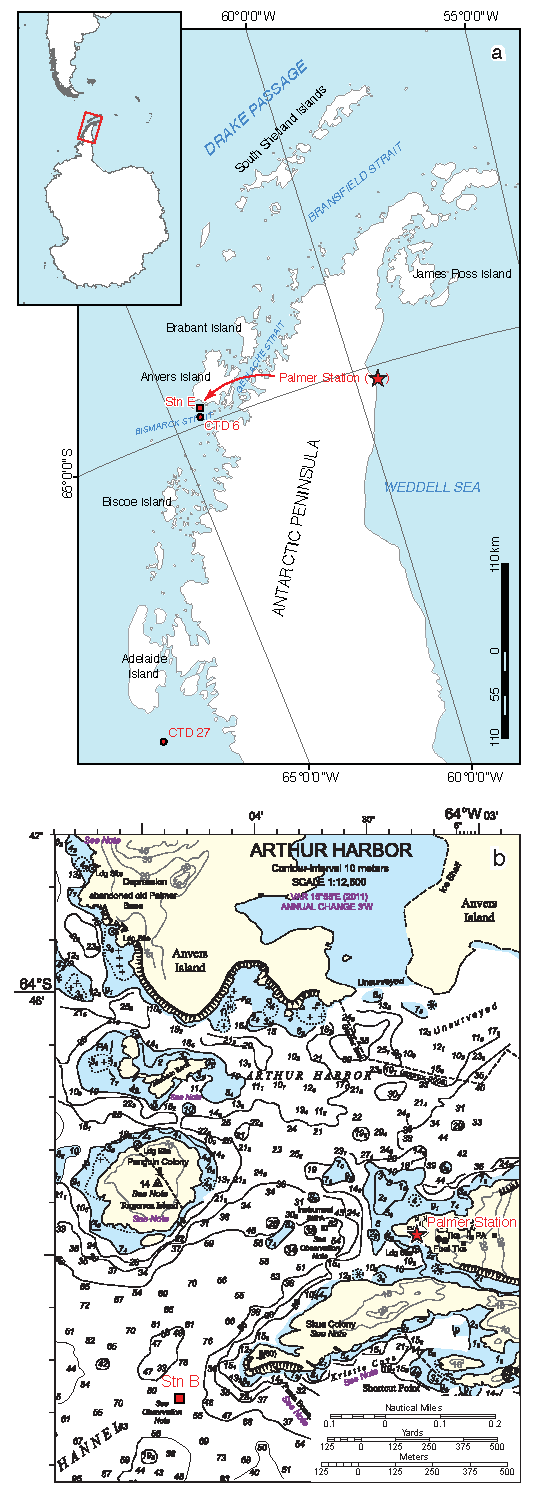
\includegraphics[width=.5\textwidth]{Fig_4-1.pdf}
\captionsetup{font={footnotesize}}
\caption[Map showing locations of sampling stations]{(a) Map of the West Antarctic Peninsula, showing locations of sampling stations referenced in the text (Palmer Long Term Ecological Research study stations B and E, 
\includegraphics[height=\fontcharht\font`\B]{images/Fig_4-Inline1.pdf}; CTD casts 6 and 27 during cruse LMG 14-01, 
\includegraphics[height=\fontcharht\font`\B]{images/Fig_4-Inline2.pdf}) and of Palmer Station (
\includegraphics[height=\fontcharht\font`\B]{images/Fig_4-Inline3.pdf}). Inset shows extent of map view in relation to Antarctica and South America. (b) Detail from inset of U.S. National Geospatial Intelligence Agency (NGA) nautical chart 29123 (INT 9105), showing bathymetry and major marine features in immediate vicinity of Palmer Station.}
\label{fig:c4n1}
\end{SCfigure}Whereas the borosilicate glass attenuated a significant fraction of incoming radiation at wavelengths \textless{} 315 nm, the quartz transmitted nearly all incoming radiation in the UVB band (290-315 nm); we thus refer hereafter to the two treatments as ``-- UVB'' and ``+ UVB,'' respectively (\autoref{fig:c4n2}). To simulate surface-layer conditions in the adjacent coastal ocean, incubations were conducted in a large, outdoor, green-bottomed aquarium at a water depth of 0.6 m. The aquarium was left open to the sky for the duration of each experiment. The station's seawater intake system was used to circulate fresh seawater through the aquarium at a rate sufficient to gently agitate the incubation vessels; the rate of circulation also served to maintain the water at a constant temperature. Samples representing various light and microbial community treatments (described below) were sacrificed in triplicate at time points throughout the day while incoming solar radiation was measured \emph{in situ}. Total exposure times in the experiments ranged from 8.2 to 12.4 hours.

\subsubsection{Preparation of Phosphatidylcholine Liposomes}

For the experiments, artificial lipid membranes were prepared from liposomes of various species of phosphatidylcholine (PC; \autoref{fig:aen1}), a membrane lipid common to nearly all phyla, including marine microbial eukaryotes and prokaryotes. The use of liposomes prepared from molecular species of the investigator's choosing allows him or her to constrain the initial composition, fate, and potential products of lipid oxidation in experiments where a high degree of control and specificity is desired (Reis and Spickett, 2012). As a consequence, liposomes are frequently used as structural analogs for membrane lipids (Wagner et al., 1994) in studies of lipid function and oxidation in both plant (e.g., Zhou et al., 2009) and human (e.g., Thomas et al., 2010) cells; more recently, a liposome model was also used to investigate the antioxidant capacity of pigments produced by a marine bacterium (Correa-Llant\'{e}n et al., 2012). Experiments with liposomes can be particularly useful in photochemical studies when distinguishing among the many pathways through which lipids can be oxidized (Stratton and Liebler, 1997).

For this study, an Avanti Mini-Extruder and seven species of synthetic phosphatidylcholine containing fatty acid moieties of varying unsaturation and chain length (full list, \autoref{table:aen1}; molecular structures, \autoref{fig:aen1}) were obtained from Avanti Polar Lipids, Inc. (Alabaster, AL, USA). To improve yield during the extruding process, liposomes were prepared from lipid films rather than from the simple dry lipid mixture recommended by the manufacturer. Detailed protocols for preparation of both films and liposomes are available online; a link is provided at the end of the manuscript. To prepare the films, known quantities of each lipid dissolved in chloroform (approx. 200 $\mu$L) were dispensed into 20 mL precombusted, round-bottomed, screw-top glass vials using a solvent-washed glass syringe. The chloroform was then evaporated under a constant stream of nitrogen gas while the vial was revolved continuously by hand around its major axis. By gradual evaporation of the chloroform in this manner, the lipid was deposited as a thin film along the inside wall of each vial. Residual chloroform was removed via vacuum centrifugation (30 minutes), the vials flushed with argon, and screw-top threads sealed with Teflon (PTFE) film. The vials were then capped and stored until needed (in all instances, \textless{} 2 months) at --20$^{\circ}$C. The final quantity of lipid in each tube ranged from 500-2000 $\mu$g, depending on the species.

Fresh liposomes were extruded from these films 1-2 hours before the start of each experiment according to a modified version of the manufacturer protocol. Briefly, for each lipid to be evaluated, a film was retrieved from cold storage and hydrated with 500 $\mu$L of a buffer solution containing 260 mM NaCl and 50 mM Tris (both reagent grade, Fisher Scientific, USA). The tube was then incubated for one hour at 60$^{\circ}$C while subjected to gentle agitation. Using the Avanti Mini-Extruder, liposomes were then extruded from the lipid suspension by forcing the suspension multiple times through a single-use 0.2 $\mu$m polycarbonate membrane. The extruder was maintained at 60-70$^{\circ}$C by means of a hot plate. The protocol was repeated for as many lipids as required. Extruder components and syringes were rinsed between use and a new membrane was used for each lipid.

\subsubsection{Experimental Design and Treatments}

A different combination of liposomes was selected for each experiment (\autoref{table:aen1}) and extruded separately as described above. The different liposome suspensions were then combined into a single volume and gently mixed. The combined suspension was then dispensed into a precombusted glass beaker containing fresh natural seawater that had been passed three times through a 0.2 $\mu$m pore size Durapore hydrophilic membrane filter (Whatman); our intent was to exclude both phytoplankton and most of the heterotrophic bacteria, while retaining any dissolved organic matter present. The raw seawater was collected from the nearby harbor by means of a peristaltic pump; tubing was flushed with a 5 \% hydrochloric acid solution prior to sampling. In two of the five experiments (20 Nov. and 14 Dec. 2013), we employed an additional seawater matrix to evaluate whether the process of microbial degradation might enhance rates of lipid photooxidation. In these experiments, we divided the liposome suspension between equal volumes of the 0.2 $\mu$m-filtered seawater and seawater which had been passed three times through a GF/F glass fiber filter (nominal pore size 0.7 $\mu$m; Whatman). In the 0.7 $\mu$m-filtered fraction, we sought to exclude the majority of large-celled eukaryotic phytoplankton. We refer hereafter to the two treatments as ``-- het. bact.'' and ``+ het. bact.,'' respectively.\begin{SCfigure}[1][!b]
\centering
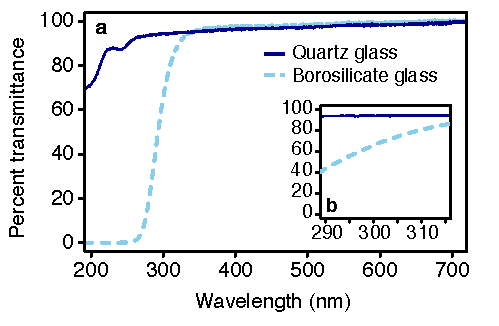
\includegraphics[width=.5\textwidth]{Fig_4-2.pdf}
\captionsetup{font={footnotesize}}
\caption[Transmission spectra of glass incubation vessels used in lipid photooxidation experiments]{(a) Transmission spectra of the glass incubation vessels used in lipid photooxidation experiments measured used a dual-path benchtop spectrophotometer. (b) Inset, showing transmissivities in the UVB spectral band (290-315 nm).}
\label{fig:c4n2}
\end{SCfigure}

After the liposome suspension was dispensed into one or both volume(s) of filtered seawater, a sufficient number of incubation vessels of the proper glass quality (quartz or borosilicate glass) were filled with the liposome-seawater solution(s) to permit evaluation in triplicate at several time points of all possible treatment combinations (-- and + UVB, and, in the case of the 20 Nov. and 14 Dec. experiments, -- and + het. bact.). To eliminate headspace, vials were filled to slightly overflowing. The mouths of the vials were then covered with PTFE film prior to stoppering (quartz vials) or securing with screw caps (borosilicate vials). Black electrical tape was used to further seal the outsides of the stoppers or screw caps to ensure vials did not inadvertently open during incubation. Sets of triplicate samples were also reserved in additional borosilicate glass vials for parallel incubation in the dark at \emph{in situ} temperature (hereafter, we refer to these as -- and + het. bact. ``dark controls'').

\subsubsection{Sampling and Extraction Protocol}

Samples were sacrificed and analyzed in triplicate at predesignated time points and the lipid content was recovered by liquid-liquid extraction. Each sample was transferred to a precombusted 200 mL glass separatory funnel and 30 $\mu$L of a synthetic IP-DAG (dinitrophenyl-phosphatidylethanolamine, or DNP-PE; Avanti) was immediately added at known concentration as an internal standard. 20 mL dichloromethane (HPLC grade; Sigma-Aldrich) was then added, followed by 50 $\mu$L of 45.4 mM butylated hydroxytoluene (BHT; 99.8 \%, Acros Organics) in HPLC-grade methanol (CHROMASOLV for HPLC; Sigma-Aldrich). This allowed us to achieve an effective concentration of the antioxidant of 0.0025\% (\emph{w/v}) in the organic phase (Yao et al., 2008). The funnel was then stoppered and mixed vigorously three times; phases were allowed to separate briefly between mixing. The organic phase (ca. 20 mL) was then collected into a precombusted glass vial and reduced in volume to approx. 1.5 mL using a nitrogen blowdown system. The final extract was transferred to a precombusted HPLC vial, topped with argon, and then stored at --80$^{\circ}$C until ready for analysis.

\subsubsection{Supplementary Assays Employed During Certain Experiments}

We employed additional assays during the 20 Nov. and 14 Dec. 2013 experiments to (1) validate our observations of lipid photooxidation with a standard measurement of lipid peroxidation and (2) interrogate bacterial metabolic activity in our + het. bact. treatments (i.e., those containing the 0.7 $\mu$m seawater filtrate). First, we adapted a commercial biomedical assay kit (ab118970 Lipid Peroxidation/MDA Assay Kit; Abcam Inc., Cambridge, UK) to detect the presence in our samples of malondialdehyde (MDA), a low-molecular-weight oxidation end-product of both enzymatically catalyzed (Armstrong and Browne, 1994) and abiotic (Janero, 1990) lipid peroxidation in a variety of organisms. The assay was carried out according to the manufacturer protocol for tissue/cell samples using 400 $\mu$L sample, 300 $\mu$L of the provided lysis buffer, and 6 $\mu$L BHT; a 510/535 nm excitation/emission filter pair was used for fluorometric detection and quantification of the MDA-thiobarbituric acid (TBA) adduct. In addition, activities of four bacterial exoenzymes (lipase, alkaline phosphatase, $\alpha$-D-glucosidase, aminopeptidase) were monitored throughout the experiments using a series of fluorogenic substrates (Hoppe, 1993) as described in Edwards et al. (2011). Briefly, pre-prepared 96-well plates containing the substrates were inoculated with aliquots of sample from each treatment; the plates were incubated in darkness at the same temperature as the water in the aquarium. The hydrolysis of these substrates and the attendant release of the free fluorophores 4-methylumbelliferone and 7-amino-4-methylcoumarin was monitored over time using a Tecan Infinite F200 Pro plate reader. External standard curves were used to convert fluorescence values to concentration units; enzyme hydrolysis rates were then calculated by linear regression from the observed changes in concentration. A detailed enzyme assay protocol and interactive MATLAB script for calculation of hydrolysis rates from raw fluorescence data are available online at \url{https://github.com/jamesrco/ExoenzymeHydroCalc}.

\subsection{Measurements of Incoming Irradiance}
\label{ssec:Measurements of Incoming Irradiance}

During the photooxidation experiments, an Ocean Optics Jaz spectrometer (ILX-511B detector; Ocean Optics Inc., Dunedin, FL, USA) was used to record incident irradiances \emph{in situ} at 0.3 nm bandwidth from 200-850 nm. Measurements were made in the aquarium at the same 0.6 m depth as the incubation vessels using an upward-facing plane irradiance cosine corrector and 5 or 10 m fiber optic cables that had been factory calibrated for absolute irradiance measurements from 210-850 nm. Irradiances were recorded at 1 min. intervals in units of $\mu$W cm\textsuperscript{-2}. The Jaz device was also used to record irradiances at 0.6 m for several extended periods from October-December 2013. Daily spectral integrals of total UVB and UVA irradiance (the time- and wavelength-integrated daily irradiance received between 290-315 nm and 315-400 nm, respectively, in a 24-hour period; reported in kJ m\textsuperscript{-2} d\textsuperscript{-1}) were calculated from these data for comparison with incident earth-surface irradiances recorded simultaneously at Palmer Station as part of the U.S. National Oceanic and Atmospheric Administration's (NOAA) Antarctic UV Monitoring Network (Bernhard et al., 2005; 2010; \autoref{fig:c4n3}).
\begin{figure}[!p]
\centering
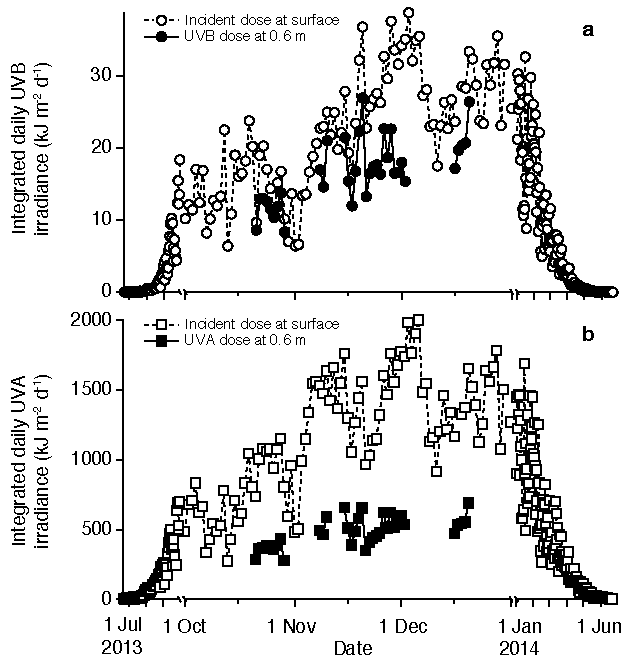
\includegraphics[width=.78\textwidth]{Fig_4-3.pdf}
\captionsetup{font={footnotesize}}
\caption[Daily doses of UVA and UVB radiation received at Palmer Station in 2013-2014]{Time- and wavelength-integrated daily doses of (a) UVB (290-315 nm) and (b) UVA (315-400 nm) radiation received at Palmer Station from 1 July 2013 to 30 June 2014. Open circles and squares: Incident doses measured at the earth surface from SUV-100 spectroradiometer data (courtesy U.S. National Oceanic and Atmospheric Administration (NOAA) Antarctic UV Monitoring Network, NOAA Global Monitoring Division, Boulder, CO, USA). Closed circles and squares (sections with expanded \emph{x}-axis): Downwelling UVB and UVA radiation received at 0.6 m below the ocean's surface, measured using a calibrated Ocean Optics Jaz spectrometer as described in the text. The largest daily dose of UVB radiation was received on 3 December 2013 even though the seasonal minimum in total column ozone (154.82 Dobson units) was recorded on 12 October 2013.}
\label{fig:c4n3}
\end{figure}

\subsubsection{Water Column Irradiance Profiles; Calculation of Downwelling Attenuation Coefficients (\emph{K\textsubscript{d}})}
\label{sssec:Water Column Irradiance Profiles; Calculation of Downwelling Attenuation Coefficients}

Finally, in 2013 and 2015, the Jaz was used to make several profiles of downwelling irradiance in the water column adjacent to Palmer Station in Arthur Harbor (e.g., \autoref{fig:c4n4}). All profiles were made at Station B, a sampling location occupied twice weekly during the austral summer as part the Palmer Long Term Ecological Research (PAL-LTER) study (\autoref{fig:c4n1}b). To achieve minimum boat shadow while making the profile measurements, the fiber optic cable and light sensor (cosine corrector) were streamed away from the small boat in a direction that was both to windward and toward the sun; the boat was then allowed to drift downwind from the measurement location to a suitable stand-off distance. Spectra were obtained at a range of depths from 0 to 8 m on days when few or no clouds were present. A series of concurrent surface irradiance measurements made with a LI-COR PAR sensor (model LI-193SA; LI-COR Biosciences, Lincoln, NE, USA) was used to correct the spectra made as part of these profiles for any changes in incident light intensity that occurred between measurements. The PAR sensor was mounted in a fixed location on the small boat such that it enjoyed a constant, unobstructed path to the sun. The corrected irradiances were used to calculate a series of wavelength-dependent downwelling attenuation coefficients, ${K_d}(\lambda )$, for wavelengths from 290-700 nm, according to:
\begin{equation} \label{eq:c4e1}
{I_z}(\lambda ) = {I_0}(\lambda ){e^{ - {K_d}(\lambda )z}}
\end{equation}
where ${I_z}(\lambda )$ is the spectral irradiance at depth $z$ and ${I_0}(\lambda )$ is the spectral irradiance just below the sea surface. Values of ${K_d}(\lambda )$ are given in \autoref{table:aen2}. Where necessary for apparent quantum yield (AQY) calculations (\autoref{ssec:Calculation of Broadband Polychromatic Apparent Quantum Yields (AQY)}, below), we also converted downwelling irradiances to wavelength-specific photon fluxes (${E_p}(\lambda )$, in units of $\mu$mol photons m\textsuperscript{-2} s\textsuperscript{-1}) using the equation
\begin{equation} \label{eq:c4e2}
{E_p}(\lambda ) = I(\lambda ) \times \lambda  \times 0.836 \times {10^{ - 2}}
\end{equation}
where $\lambda$ is a given wavelength in nm, ${I}(\lambda )$ is the irradiance in W m\textsuperscript{-2}, and the additional numerical coefficients are used to effect necessary conversions via Planck's equation and Avogadro's number.
\begin{figure}[!t]
\centering
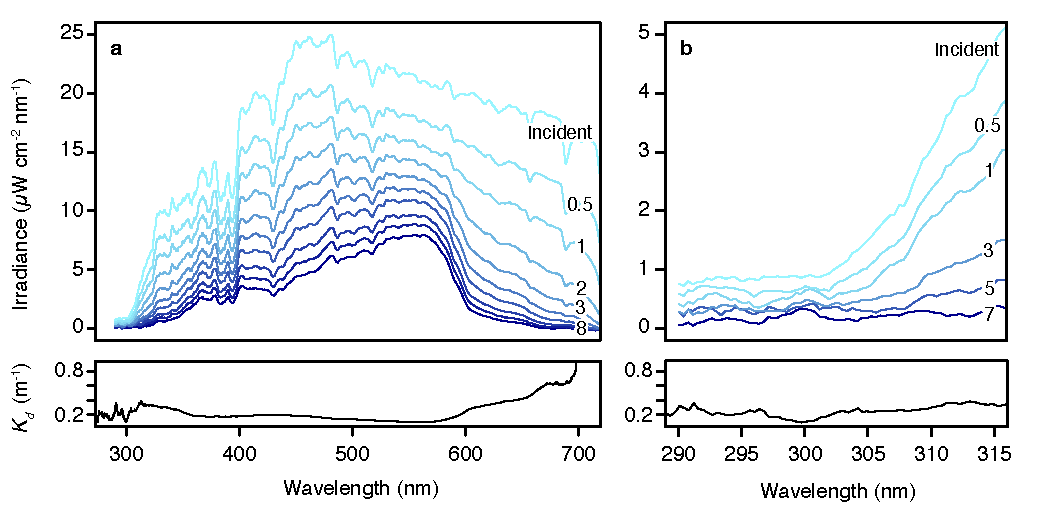
\includegraphics[width=1\textwidth]{Fig_4-4.pdf}
\captionsetup{font={footnotesize}}
\caption[Wavelength-specific measurements of downwelling irradiance in Arthur Harbor]{Wavelength-specific measurements of downwelling irradiance in Arthur Harbor (PAL-LTER Station B) on 15 December 2015. Labels refer to depths in meters below the sea surface. (a) UV-visible spectra (290-700 nm) at 10 depths. Data from 1-8 m are plotted at 1 m intervals. (b) Inset showing UVB-band (290-315 nm) irradiances at selected depths. Bottom panels show downwelling attenuation coefficients for each wavelength, ${K_d}(\lambda )$, which were calculated from the data according to \autoref{eq:c4e1} in the text. ${K_d}(\lambda )$ for wavelengths 280-700 nm are given in \autoref{table:aen2}.}
\label{fig:c4n4}
\end{figure}

\subsection{Benchtop Absorbance and Transmissivity Measurements}
\label{ssec:Benchtop Absorbance and Transmissivity Measurements}

Wavelength-specific absorbances of various PC lipid standards (dissolved in HPLC-grade methanol; \autoref{fig:c4n5}) and seawater samples from surface waters in Arthur Harbor (\autoref{fig:aen2}) were measured in the laboratory using a dual-path UV-visible spectrophotometer (Thermo Nicolet Evolution 300; ThermoFisher Scientific). 100 mm quartz cuvettes were used for all measurements. HPLC-grade methanol and 0.2 $\mu$m-filtered oligotrophic ocean seawater (collected from 50 m at the Bermuda-Atlantic Time Series site, 32$^{\circ}$ 10' N, 64$^{\circ}$ 30' W) were used as references for the two sample types, respectively. Absorbance spectra of the liposome standards (\autoref{fig:c4n5}a,b) were used to calculate wavelength-specific decadic molar extinction coefficients (${\varepsilon _i}(\lambda )$, in units of M\textsuperscript{-1} cm\textsuperscript{-1}; \autoref{fig:c4n5}c) using the equation
\begin{equation} \label{eq:c4e3}
{\varepsilon _i}(\lambda ) = {A_i}(\lambda ) \times {C_i} \times \ell 
\end{equation}
where ${A_i}(\lambda )$ is the absorption at wavelength $\lambda$, $\ell$ is the pathlength (10 cm), and ${C_i}$ is the concentration of the relevant analyte (liposome standard) in units of mol L\textsuperscript{-1}. Raw absorbances of the seawater samples (${A_{SW}}(\lambda )$) were used to calculate wavelength-specific seawater absorbance coefficients (${a_{SW}}(\lambda )$, in units of m\textsuperscript{-1}; \autoref{fig:aen2}) according to:
\begin{equation} \label{eq:c4e4}
{a_{SW}}(\lambda ) = {A_{SW}}(\lambda ) \times 2.303/\ell 
\end{equation}
Transmission spectra of the glass incubation vessels (\autoref{ssec:UV Photooxidation Experiments}, above; \autoref{fig:c4n2}) were recorded using the same instrument on which the liposome and seawater absorbance spectra were acquired.

\subsection{Laboratory Determination of H\textsubscript{2}O\textsubscript{2} and O\textsubscript{2}\textsuperscript{-} Photoproduction and Decay}
\label{ssec:Laboratory Determination of ROS Photoproduction and Decay}

In a series of subsequent experiments in the laboratory in Woods Hole, net hydrogen peroxide (H\textsubscript{2}O\textsubscript{2}) and superoxide (O\textsubscript{2}\textsuperscript{-}) photoproduction rates were estimated in surface seawater samples from Arthur Harbor. H\textsubscript{2}O\textsubscript{2} concentrations were determined using the colorimetric Ampliflu Red method described in Zhang et al. (2016a). O\textsubscript{2}\textsuperscript{-} concentrations were measured with a continuous-flow FeLume Mini system (Waterville Analytical, Waterville, ME, USA) configured as described in Zhang et al. (2016b). In the experiments, previously frozen, 0.7 $\mu$m-filtered seawater samples were excited at a series of wavelengths using the spectrophotometer described in \autoref{ssec:Benchtop Absorbance and Transmissivity Measurements}; concentrations of H\textsubscript{2}O\textsubscript{2}) and superoxide (O\textsubscript{2}\textsuperscript{-} were then measured using the methods described above. To evaluate photoproduction rates of H\textsubscript{2}O\textsubscript{2}, we excited samples at 280, 310, and 360 nm based on the findings of Kieber et al. (2014); for O\textsubscript{2}\textsuperscript{-}, we evaluated a broader wavelength range (50-nm-wavelength increments from 300-500 nm; Powers and Miller, 2015). Sample water was passed through beam of the spectrophotometer using a peristaltic pump and 10 mm pathlength flow-cell while the xenon lamp was operated in continuous (i.e., not flash) mode at the desired wavelength. Opaque (black) tubing was used, and all other components were triple-shielded using aluminum foil. Downstream of the spectrophotometer beam, the sample was either pumped directly into the FeLume (for O\textsubscript{2}\textsuperscript{-}) or expediently assayed for H\textsubscript{2}O\textsubscript{2}. The intensity of the xenon lamp output in the UVB range (determined using the Jaz spectrometer described in \autoref{sssec:Water Column Irradiance Profiles; Calculation of Downwelling Attenuation Coefficients}) was roughly equivalent to the downwelling UVB irradiances we observed at 1 m in Arthur Harbor (the lamp output at 290 nm was 0.43 $\mu$W cm\textsuperscript{-2}, compared with 0.42 $\mu$W cm\textsuperscript{-2} at 1 m in the profile presented in \autoref{fig:c4n4}). At wavelengths \textgreater{} 315 nm, the spectrophotometer output was significantly less intense than what was observed in the water column. In a final set of experiments, the ability of Arthur Harbor seawater to quench (i.e., degrade) H\textsubscript{2}O\textsubscript{2} and O\textsubscript{2}\textsuperscript{-} was estimated by measuring concentrations of the two ROS after spiking the samples with progressively larger concentrations of potassium superoxide (KO\textsubscript{2}).
\begin{SCfigure}[1][!t]
\centering
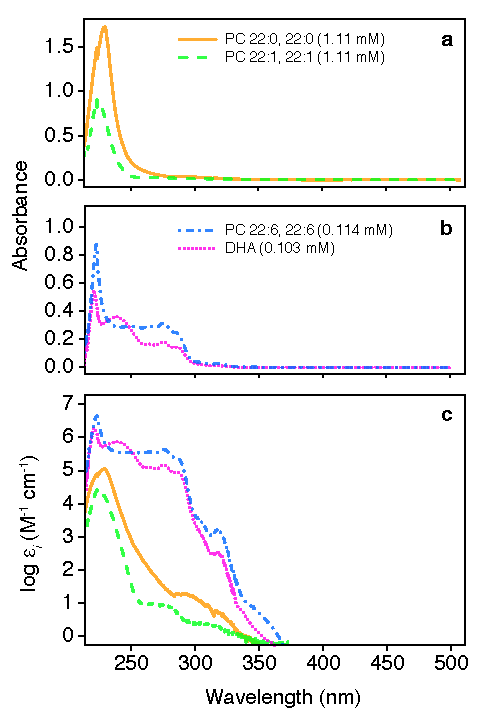
\includegraphics[width=.56\textwidth]{Fig_4-5.pdf}
\captionsetup{font={footnotesize}}
\caption[Wavelength-specific absorbances and decadic molar extinction coefficients of phosphatidylcholine and DHA]{Effect of acyl unsaturation on photochemical potential in the membrane lipid phosphatidylcholine (PC) and constituent fatty acid docosahexaenoic acid (DHA). (a) Wavelength-specific absorbances of equimolar (1.11 mM) concentrations of PC 22:0, 22:0 and PC 22:1, 22:1 (\emph{cis}-$\Delta$\textsuperscript{13}) dissolved in methanol. (b) Wavelength-specific absorbances of PC 22:6, 22:6 (\emph{all-cis}-$\Delta$\textsuperscript{4},$\Delta$\textsuperscript{7},$\Delta$\textsuperscript{10},$\Delta$\textsuperscript{13},$\Delta$\textsuperscript{16},$\Delta$\textsuperscript{19}) and DHA at concentrations in methanol of 0.114 and 0.103 mM, respectively. (c) Decadic molar extinction coefficients, ${\varepsilon _i}(\lambda )$, for the four species, calculated according to \autoref{eq:c4e3} in the text. Note logarithmic scale on the \emph{y}-axis.}
\label{fig:c4n5}
\end{SCfigure}

\subsection{Water Column Sample Collection}

In addition to the photooxidation experiments, several water samples were collected for lipid analysis in 2013-2014 from waters of the adjacent harbor (at LTER Station B; \autoref{fig:c4n1}b) and on an oceanographic research cruise off the West Antarctic Peninsula (PAL-LTER cruise LMG1401 aboard the \emph{R/V Laurence M. Gould}). Persistent sea ice in the immediate vicinity of Palmer Station prevented regular collection of samples there until mid-December 2013; samples from the \emph{Gould} cruise were collected in January 2014 at distances of 50-300 km from shore. Samples for analysis of particulate (i.e., cell-bound) lipids were retrieved from depth using standard oceanographic sampling equipment and then collected by vacuum filtration onto 0.2 $\mu$m pore size Durapore membrane filters; these were frozen immediately at --80$^{\circ}$C. For analysis of total lipids, we used the liquid-liquid method described above to extract 2000 mL of seawater into 200 mL dichloromethane in a 2 L separatory funnel; 120 $\mu$L of DNP-PE and 100 $\mu$L BHT were added as internal standard and preservative antioxidant, respectively. Extraction of particulate samples was performed using a modified Bligh and Dyer (Bligh and Dyer, 1959) method described in Popendorf et al. (2013). Extracts were processed and then stored at --80$^{\circ}$C as described above.

\subsection{High-Resolution HPLC-ESI-MS Analysis}

Lipid extracts were analyzed by HPLC-ESI-MS with data dependent-MS\textsuperscript{2} acquisition on a high-resolution, accurate mass Thermo Q Exactive Hybrid Quadrupole-Orbitrap mass spectrometer (ThermoFisher Scientific, Waltham, MA, USA) coupled to an Agilent 1200 HPLC system (Agilent, Santa Clara, CA, USA) comprising a temperature-controlled autosampler (4$^{\circ}$C), binary pump, and diode array detector. Chromatographic conditions were modified from Hummel et al. (2011). High-resolution mass data were acquired in both positive and negative ionization modes; following the full spectrum scan in each mode, the five ions of highest intensity were selected using the quadrupole for MS\textsuperscript{2} fragmentation. Full details, including chromatographic conditions, electrospray ionization source settings, MS acquisition settings, and mass spectrometer calibration procedures, are described in the Supporting Information (\autoref{ssec:Mass Spectrometer Acquisition Settings}); the method allowed us to achieve an effective mass accuracy of \textless{} 0.2 ppm, as reported in Collins et al. (2016). All chemicals used in sample extraction and chromatography were LC/MS grade or higher. Where used, water was obtained from a Milli-Q system without further treatment (EMD Millipore, Billerica, MA, USA).

\subsubsection{Identification and Quantification of Lipids \& Oxidized Lipids}
\label{sssec:Chap 4 - Identification and Quantification of Lipids and Oxidized Lipids}

HPLC-ESI-MS data were processed in R (R Core Team, 2016) using msConvert (Kessner et al., 2008), xcms (Benton et al., 2010; C. A. Smith et al., 2006; Tautenhahn et al., 2008), and CAMERA (Kuhl et al., 2012) according to the steps described in Collins et al. (2016). The R package IPO (Libiseller et al., 2015) was used to optimize some xcms settings. The LOBSTAHS lipidomics discovery software (Collins et al., 2016) was used to extract and putatively identify MS features in both the experimental and environmental data. In data from the liposome experiments, we identified the added PC species, any possible degradation products, and the internal standard, DNP-PE. For intact PC species, DNP-PE, and constituent fatty acids, we confirmed each LOBSTAHS identification using two additional means: (1) via comparison of data-dependent MS\textsuperscript{2} spectra with those from authentic standards or published reference spectra and (2) by requiring the presence of the same compound identity in data acquired in the opposite HPLC-ESI-MS ionization mode. We confirmed the basic identities of the LPC and ox-PC species based on the presence of four or more diagnostic PC headgroup fragments in the relevant MS\textsuperscript{2} spectrum. In the more complex environmental samples and in single-species culture data, we confirmed all LOBSTAHS identities at the lipid class level (e.g., PC versus PE, or MGDG versus TAG) using a new, experimental LOBSTAHS feature which automatically detects diagnostic product ion fragments and constant neutral losses (as given in Popendorf et al., 2013) in the available data-dependent MS\textsuperscript{2} spectra for each sample. In addition, we required the presence of the same LOBSTAHS compound identity in data acquired in the opposite HPLC-ESI-MS ionization mode, as described above for the experimental data.

After identification, quantification of analytes was performed using a series of standard curves. For quantification of IP-DAG, authentic standards were obtained either from natural extracts or from the same source (Avanti Polar Lipids) as the lipids used in the liposomes (Popendorf et al., 2013; Van Mooy and Fredricks, 2010). For quantification of docosahexaenoic acid (DHA), an authentic standard was obtained from Nu-Chek Prep Inc. (Elysian, MN, USA). For LPC and ox-PC species, we applied the standard curve for the corresponding intact, unoxidized molecule; authentic standards are commercially available for only a small fraction of the many possible intact ox-PC species and their isomers. The concentration of each analyte was then normalized to the concentration in the same sample of the internal standard.

\subsection{Calculation of Broadband Polychromatic Apparent Quantum Yields (AQY)}
\label{ssec:Calculation of Broadband Polychromatic Apparent Quantum Yields (AQY)}

We combined the removal rates (where observed) of PC species determined in the liposome experiments, \emph{in situ} photon flux measurements, and other parameters described above to calculate a series of broadband (as in, e.g., Fichot and Benner, 2014) polychromatic apparent quantum yields, ${\Phi _{{\lambda _1}:{\lambda _2}}}$, where
\begin{singlespace}
\begin{equation} \label{eq:c4e5}
{\Phi _{{\lambda _1}:{\lambda _2}}} = \frac{{{\text{moles of a given lipid }}i{\text{ transformed}}}}{\begin{gathered}
  {\text{no. of moles of photons between wavelenths }} \\ 
  {\lambda _1}{\text{ and }}{\lambda _{\text{2}}}{\text{ absorbed due to the presence of }}i \\ 
\end{gathered} }
\end{equation}
\end{singlespace} 
\hfill\break
We calculated these yields according to the equation:
\begin{equation} \label{eq:c4e6}
{\Phi _{{\lambda _1}:{\lambda _2}}} = \frac{{\frac{{ - d[i]}}{{dt}}}}{{[i]\int\limits_{{\lambda _1}}^{{\lambda _2}} {{K_s}(\lambda )d\lambda } }}
\end{equation}
where ${\Phi _{{\lambda _1}:{\lambda _2}}}$ is the broadband polychromatic AQY in units of mol (mol photons)\textsuperscript{-1}, $ - d[i]/dt$ is the change in concentration of lipid \emph{i} in a given experimental treatment, $[i]$ is the concentration of \emph{i} measured in the experiment at \emph{t} = 0 (i.e., prior to photon exposure), and ${K_s}(\lambda )$ are the time-integrated specific absorbances of \emph{i} calculated at wavelengths from ${\lambda _1}$ to ${\lambda _2}$. Our experimental design allowed us to calculate AQY for three wavelength ranges: ${\Phi _{290:315}}$ (or ${\Phi _{UVB}}$, for radiation received in the UVB band), ${\Phi _{315:395.5}}$ (${\Phi _{UVA}}$, for radiation received in the UVA band), and ${\Phi _{290:395.5}}$ (or ${\Phi _{UVR}}$, a yield based on the total received UV radiation).

We used a different definition of $ - d[i]/dt$ for calculation of the three AQY; these hewed closely to the observed transmittance spectra of the various treatment vessels (\autoref{fig:c4n2}). In all three cases, we assumed the change in concentration of PC 22:6, 22:6 in the dark control treatment (-39 $\pm$ 23 pmol mL\textsuperscript{-1} hr\textsuperscript{-1}; \autoref{table:c4n1} and \autoref{fig:c4n6}a) represented the baseline rate of autooxidation, a process common to all lipids containing unsaturated acyl moieties but often more significant in those containing highly polyunsaturated fatty acids (Girotti, 1998). For ${\Phi _{UVR}}$, we therefore defined $ - d[i]/dt$ as the change in concentration observed in the +UVB (quartz glass) treatment relative to the change in the dark control. For calculation of ${\Phi _{UVA}}$, we applied the concentration change observed in the --UVB (borosilicate glass) treatment, again correcting for the dark oxidation rate. Finally, for calculation of ${\Phi _{UVB}}$, the efficiency of photooxidation attributable only to UVB radiation, we defined $ - d[i]/dt$ as the difference between the changes in concentration observed in the -- UVB and + UVB treatments. ${K_s}(\lambda )$ were calculated after Pereira et al. (2007) according to the equation
\begin{equation} \label{eq:c4e7}
{K_s}(\lambda ) = \frac{{E_{p,\Sigma }^o(\lambda )T(\lambda ){\varepsilon _i}(\lambda )(1 - {{10}^{ - {a_{SW}}(\lambda ){z_{eff}}}})}}{{{a_{SW}}(\lambda ){z_{eff}}}}
\end{equation}	
where $E_{p,\Sigma }^o(\lambda )$ is the total number of photons of wavelength $\lambda$ received per unit area over the course of the experiment, i.e.,
\begin{equation} \label{eq:c4e8}
E_{p,\Sigma }^o = \int\limits_{t = 0}^{t = f} {E_p^o(\lambda )dt} 
\end{equation}	
$T(\lambda )$ is the transmissivity (as a fraction) of the incubation vessel wall material at wavelength $\lambda$, ${\varepsilon _i}(\lambda )$ is the experimentally-determined decadic molar extinction coefficient at wavelength $\lambda$ (from \autoref{eq:c4e3}), and ${a_{SW}}(\lambda )$ and $(1 - {10^{ - {a_{SW}}(\lambda ){z_{eff}}}})$ are the wavelength-specific absorbance coefficient (m\textsuperscript{-1}) and fraction of radiation absorbed by the seawater in the incubation vessel along the effective path length ${z_{eff}}$, respectively. For ${z_{eff}}$, we applied one-half the inner diameter of the incubation vessels ($0.5\times2$ cm = 1 cm) since the vessels were left to rest almost exclusively on their sides during the experiments and were exposed to sunlight from above.

\subsubsection{Determination of Uncertainties in AQY Estimates}
\label{sssec:Determination of Uncertainties in AQY Estimates}

We used a series of Monte Carlo-style computational simulations to determine uncertainties in our final estimates of AQY. The method used was similar to that described in Collins et al. (2015). First, where possible, we determined uncertainties for all individual parameters in \autoref{eq:c4e6}, \autoref{eq:c4e7}, and \autoref{eq:c4e8} from experimental replication or, in the case of data obtained from single samples using the benchtop spectrophotometer, repeated analytical measurements. We then conducted a series of 10,000 simulations in which a new value for each parameter was chosen at random from a normal distribution constructed from the parameter's mean value and analytical or observational uncertainty as its standard deviation. In each simulation, the randomly chosen values from these normal distributions were used to obtain a different estimate of the AQY from \autoref{eq:c4e6}, \autoref{eq:c4e7}, and \autoref{eq:c4e8}. The final uncertainty in each AQY estimate was determined from the standard deviation of the set of estimates generated during the simulation. The R code we used to conduct the simulation is available online; a link is provided in the Supporting Information. Although we constructed normal distributions for each parameter in the simulations, we could not be absolutely certain the underlying populations were normally distributed because of the small sample sizes.

\subsection{Lipid Photooxidation Rate Estimates}

Finally, we estimated rates of lipid photooxidation in natural waters of the West Antarctic Peninsula by combining our estimates of AQY with direct observations of subsurface irradiance and measured concentrations of specific lipids. Rates were estimated for two fractions of the lipids we measured in WAP waters: IP-DAG containing (1) polyunsaturated (i.e., $\geq$ 3 double bonds) and (2) highly polyunsaturated (i.e., $\geq$ 5 double bonds) fatty acids at both positions (\emph{sn-­}1 and \emph{sn-}2) on the IP-DAG glycerol backbone. Photooxidation rates ($ - d[i]/dt$; units of pmol lipid or pmol C d\textsuperscript{-1}) were calculated according to \autoref{eq:c4e6}, where ${\Phi _{{\lambda _1}:{\lambda _2}}}$ was the broadband polychromatic AQY for the UVB spectrum (${\Phi _{290:315}}$, or ${\Phi _{UVB}}$) and $[i]$ was the measured concentration (in pmol L\textsuperscript{-1}) of lipids in the respective fraction. We calculated the necessary ${K_s}(\lambda )$ according to
\begin{equation} \label{eq:c4e9}
{K_s}(\lambda ) = \frac{{E_{p,\Sigma }^o(\lambda ){\varepsilon _i}(\lambda )(1 - {{10}^{ - {K_d}(\lambda ){z_{surf}}}})}}{{{K_d}(\lambda ){z_{surf}}}}
\end{equation}	
where $E_{p,\Sigma }^o(\lambda )$ was a daily flux ($\mu$mol photons m\textsuperscript{-2} d\textsuperscript{-1}) calculated from the time-series of \emph{in situ} irradiance measurements described in \autoref{ssec:Measurements of Incoming Irradiance}, ${\varepsilon _i}(\lambda )$ was the experimentally-determined decadic molar extinction coefficient for the unsaturated compound, PC 22:6, 22:6, at wavelength $\lambda$, ${K_d}(\lambda )$ was the appropriate downwelling attenuation coefficient for Arthur Harbor calculated in \autoref{eq:c4e1}, and ${z_{surf}}$ was the depth of the well-mixed surface layer (5 m). We applied the measured ${\varepsilon _i}(\lambda )$ for PC 22:6, 22:6 to all lipids containing multiple polyunsaturated fatty acids based on our observations of the effect of polyunsaturation on specific absorbance in IP-DAG (\autoref{fig:c4n5}); in addition, it would have been highly impractical within the scope of the present work to measure specific ${\varepsilon _i}(\lambda )$ for the hundreds of different IP-DAG we observed in the natural samples.

\section{Results}
\subsection{Irradiance Observations; UV Penetration Through Shallow Mixed Layer}
\label{ssec:Irradiance Observations; UV Penetration Through Shallow Mixed Layer}

Comparison of daily UVB-band integrals calculated from our \emph{in situ} data (\autoref{fig:c4n3}a, filled circles) with integrals calculated from the incident NOAA data (\autoref{fig:c4n3}a, open circles) indicated that 70 $\pm$ 11 \% of the UVB radiation received at the earth's surface reached the 0.6 m depth at which we conducted our experiments (mean $\pm$ SD of 35 daily observations). A parallel calculation using UVA-band integrals indicated that 37 $\pm$ 3 \% of incident UVA radiation was received at 0.6 m (\autoref{fig:c4n3}b). While these findings are inconsistent with evidence from the majority of marine systems that UVB radiation is attenuated more rapidly with depth than lower-energy UVA radiation (Tedetti and Semp\'{e}r\'{e}, 2006), Figueroa (2002) found that ${K_d}(\lambda )$ for UVA wavelengths exceeded those for UVB wavelengths at two coastal sites very near Palmer Station.

Our profile measurements of downwelling irradiance (\autoref{fig:c4n4}) indicated that much of the UVB radiation at wavelengths \textless{} 300 nm was quickly attenuated in the water column; however, some UVB and a significant proportion of UVA radiation penetrated to depths of \textgreater{} 5 m. Our data confirm the findings of Moreau et al. (2015), who found that ecologically relevant doses of UVB radiation (i.e., doses $\geq$ 1 \% of surface intensity, the same standard used for determination of euphotic zone depth) were received at depths as great as 12 m in some West Antarctic Peninsula waters. Perhaps most importantly, this optical penetration was sufficient to expose nearly all of the shallow early-season mixed layer (\autoref{fig:aen3}) to robust doses of UV radiation throughout the study period. Typical mid-season mixed layer depths in Arthur Harbor range from 10-20 m (Tortell et al., 2014). Yet shallow MLDs of just 5-10 m, such as those we observed in 2013, are not unusual in the early spring following the breakup and retreat of the sea ice, which can create a highly stratified surface layer that traps both nutrients and ice-attached algae at the ocean's surface as they are released from the melting ice (Perrette et al., 2011; W. O. Smith and Nelson, 1985; 1986). A comparable surface lens may also be present throughout the season in coastal waters that receive significant inputs of glacial meltwater and in offshore waters at the persistent marginal ice zone (Carvalho et al., 2016; Huang et al., 2012). CTD profiles from PAL-LTER Station B (\autoref{fig:aen3}) indicate that the 2013-2014 season was not atypical in this regard, although the ice retreat occurred much later than usual.
\begin{SCfigure}[1][!t]
\centering
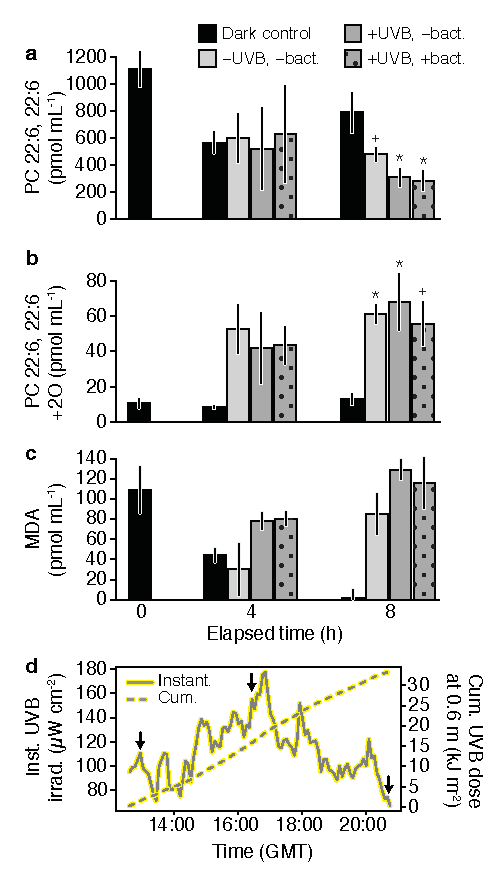
\includegraphics[width=.6\textwidth]{Fig_4-6.pdf}
\captionsetup{font={footnotesize}}
\caption[Results from a lipid photooxidation experiment conducted with phosphatidylcholine (PC) liposomes]{Results from a lipid photooxidation experiment conducted with phosphatidylcholine (PC) liposomes at Palmer Station on 14 December 2013. Concentrations after 4 and 8 h of (a) PC 22:6, 22:6, (b) an intact oxidation product (PC 22:6, 22:6 +2O; identified at chromatographic retention time 10.4 min.), and (c) malondialdehyde, a commonly-used indicator of lipid peroxidation activity. Error bars: $\pm$ SE of mean (initial concentrations, \emph{N} = 4 replicates; all other treatments and time points, \emph{N} = 3). Symbols in (a) and (b) indicate statistical significance of mean from initial concentration (value at \emph{t} = 0) according to Tukey's ``Honest Significant Difference'' method with $\alpha$ = 0.05: \emph{p} $\leq$ 0.05 (+), \emph{p} $\leq$ 0.01 (*). (d) Instantaneous (solid line) and cumulative (dashed line) UVB-band downwelling irradiance measured at the incubation depth (0.6 m). Arrows in (d) correspond to the times in (a)-(c) at which samples were sacrificed.}
\label{fig:c4n6}
\end{SCfigure}

\subsection{Rates of Photooxidation in Phosphatidylcholine Liposome Experiments}

Rates of photooxidation under exposure to natural sunlight were statistically significant in only one of the seven PC species we considered in our liposome experiments: PC 22:6, 22:6 (\emph{all-cis}-$\Delta$\textsuperscript{4},$\Delta$\textsuperscript{7},$\Delta$\textsuperscript{10},$\Delta$\textsuperscript{13},$\Delta$\textsuperscript{16},$\Delta$\textsuperscript{19}) (\autoref{fig:c4n6}a, showing results from experiment on 14 December 2013). Photooxidation rates of 80 $\pm$ 16, 98 $\pm$ 17 and 100 $\pm$ 17 pmol mL\textsuperscript{-1} hr\textsuperscript{-1} of the molecule were observed in the --UVB --het. bact., +UVB --het bact., and +UVB +het. bact. treatments, respectively (mean $\pm$ SE; \autoref{table:c4n1}). While we observed no statistical difference between these three rates, the rates in all three treatments were significantly different than the rate observed in the control treatment, 39 $\pm$ 23 pmol mL\textsuperscript{-1} hr\textsuperscript{-1} (\emph{p} $\leq$ 0.05; \autoref{table:c4n1}). In a second experiment for which results were not statistically significant (\autoref{table:aen1}), we recorded a photooxidation rate for liposomes of the same molecule of 57 $\pm$ 45 pmol mL\textsuperscript{-1} hr\textsuperscript{-1} in the +UVB --het bact. treatment. The consistently negative results we observed in the six other molecular species were confirmed in each case in at least two independent experiments (\autoref{table:aen1}). Differences in photooxidation rates were assessed within each experiment using Tukey's ``Honest Significant Difference'' method ($\alpha$ = 0.05), which takes into account the total variance in an experimental dataset when making multiple, simultaneous pairwise comparisons among treatments and timepoints (Yandell, 1997). Based on concentrations of PC 22:6, 22:6 observed in \emph{t} = 0 samples from the experiment for which we present results in \autoref{fig:c4n6} and \autoref{table:c4n1}, we recovered 80.5 \% of our starting lipid film as liposomes (\emph{t} = 0 concentration, 1108 $\pm$ 125 pmol mL\textsuperscript{-1}; calculated concentration based on known mass of lipid film, 1376.1 pmol mL\textsuperscript{-1}).

\subsection{Role and Activity of Heterotrophic Bacteria}
\subsubsection{No Evidence for Direct Bacterial Metabolism of Unoxidized Lipids}
\begin{figure}[!p]
\centering
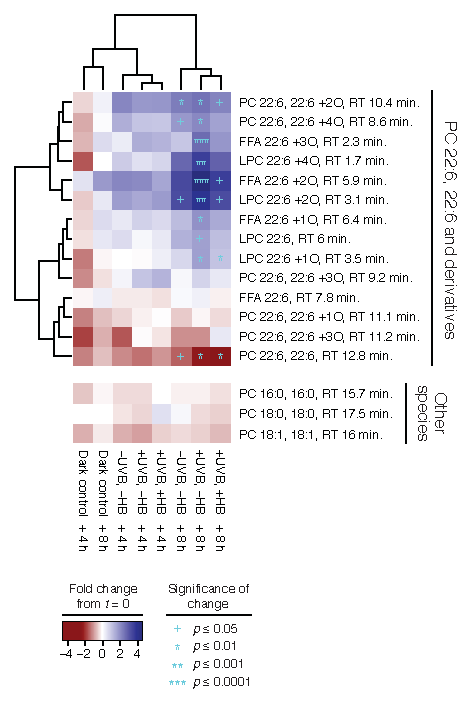
\includegraphics[width=.8\textwidth]{Fig_4-7.pdf}
\end{figure}

We observed a small marginal enhancement in the apparent degradation rate of PC 22:6, 22:6 liposomes in the +UVB treatment when heterotrophic bacteria were present, but this increase was not statistically significant (\autoref{fig:c4n6}a; \autoref{table:c4n1}). We had initially hypothesized that (1) bacterial metabolism of intact lipids present in the liposomes might enhance apparent overall degradation rates as the organisms responded to the addition of a new potential food source and that (2) bacterial metabolism might be further stimulated by photodegradation of the added lipids into smaller, less complex metabolites that could be more readily assimilated as substrates for growth. Several studies (e.g., Karl and Resing, 1993; D. J. Kieber et al., 1989) have suggested that photochemical degradation of dissolved organic matter in the surface ocean can stimulate the microbial loop by breaking down large, biologically refractory molecules into smaller, more bioavailable components. Despite some evidence that high doses of UVR can severely inhibit rates of metabolism in marine heterotrophic bacteria (Santos et al., 2011), two thorough reviews of the relevant literature (Jeffrey et al., 2000; Moreau et al., 2016) suggest that no single generalization can be made about the effect of ultraviolet radiation on marine bacterial communities: The \begin{figure} [!t]
\captionsetup{font={footnotesize}}
\captionof{figure}[Changes in the concentration of PC 22:6, 22:6 and various molecular derivatives during the liposome photooxidation experiment presented in \autoref{fig:c4n6}]{(preceding page) Changes in the concentration of PC 22:6, 22:6 and various molecular derivatives during the liposome photooxidation experiment presented in \autoref{fig:c4n6}. For a given treatment and time point on the \emph{x}-axis, cell color shows the fold change in concentration of each molecule on the \emph{y}-axis relative to the concentration observed at the initial experimental timepoint. Fold-change calculations are based on mean concentrations measured at each treatment and time point in at least 3 replicates. The order of both rows (analytes) and columns (treatment-time point combinations) reflects application of an unsupervised clustering algorithm. The dendrogram shows similarity (by Euclidean distance) among analytes and treatments/time points. Symbols in cyan indicate the statistical significance of the difference of each mean concentration relative to the mean concentration at the initial time point according to Tukey's ``Honest Significant Difference'' method with $\alpha$ = 0.05: \emph{p} $\leq$ 0.05 (+), \emph{p} $\leq$ 0.01 (*), \emph{p} $\leq$ 0.001 (**), \emph{p} $\leq$ 0.0001 (***). The lower subplot shows changes in concentration observed in the other PC species evaluated in the same experiment; no significant changes were observed in any of the species containing fully saturated or monounsaturated fatty acids. The heatmap was generated in R (R Core Team, 2016) using the gplots (Warnes et al., 2016) package.}
\label{fig:c4n7}
\end{figure}correlations (or lack thereof) observed in a given marine ecosystem between bacterial metabolism and the quantity or intensity of UVR are determined by the interaction of several complex biological, chemical and physical processes, any of which may operate in opposition to one another. Accordingly, we could find no direct evidence to support our first hypothesis that bacteria would directly degrade the liposomes. We observed no statistically significant enhancement of bacterial exoenzyme activities in either of the +het. bact. treatments compared with the basal activities we observed in dark vials containing 0.7 $\mu$m filtered seawater (Tukey HSD test with $\alpha$ = 0.05; not shown). This negative result extended to the activity of lipase, an enzyme in which we would have expected to see an increase in activity if significant numbers of bacteria were attempting to directly access carbon in intact IP-DAG. It is possible we did not observe any significant hydrolysis of the lipase activity indicator (4-methylumbelliferone-butyrate-heptanoate-palmitate) because of competition between the substrate and the liposomes themselves.

\subsubsection{Some Support for Bacterial Metabolism of Oxidized Degradation Products}
\label{sssec:Some Support for Bacterial Metabolism of Oxidized Degradation Products}

We did find some indirect evidence in our results to support the second hypothesis, i.e., that photooxidation could stimulate bacterial metabolism via degradation of intact lipids into smaller, more labile components. For example, in comparing the +UVB --het. bact. treatment to the corresponding +UVB treatment that included heterotrophic bacteria, we noted greater and more significant net production rates in the former of nearly all the PC 22:6, 22:6 degradation products that we could identify in our HPLC-MS data (compare rightmost two columns in \autoref{fig:c4n7}). Assuming the gross rate of photooxidation in the two treatments was the same, one possible interpretation of these results is that some fraction of the oxidized compounds produced in the +het. bact. treatment was removed via heterotrophic metabolism. This interpretation is challenged by recent work showing heterotrophic bacteria cannot use oxylipins such as polyunsaturated aldehydes (PUA) --- the highly bioactive derivatives of fatty acids that are considered the ``terminal'' products of lipid peroxidation --- as a viable food source (Edwards et al., 2015; Ribalet et al., 2008). However, these studies did not evaluate the ability of heterotrophic bacteria to metabolize any of the many other compounds, such as LPC or intact ox-PC species, which we show here can be produced as intermediates in the course of photooxidation (\autoref{fig:c4n7}). There is evidence that marine bacteria can use simpler aldehydes as a carbon source (Sun et al., 2011), while the bacterial metabolisms of ox-IPL and lysophosopholipids have not been specifically investigated.

\subsection{Malondialehyde Assay Results Generally Confirm Other Findings}
\begin{figure}[!t]
\centering
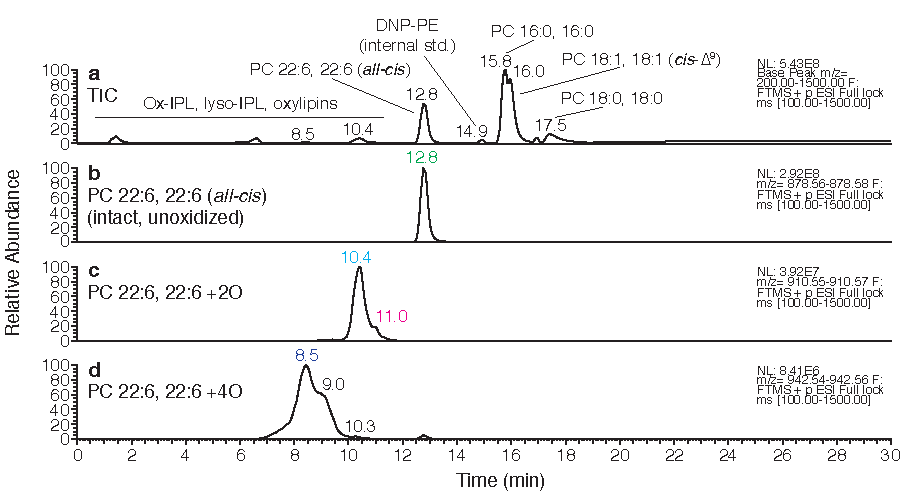
\includegraphics[width=1\textwidth]{Fig_4-8.pdf}
\captionsetup{font={footnotesize}}
\caption[Lipids and oxidized lipids identified in the lipid photooxidation experiment presented in \autoref{fig:c4n6}]{Lipids and oxidized lipids identified in a lipid photooxidation experiment on 14 December 2013. (a) Total ion chromatogram showing all lipids identified in one of three replicate samples of the + UVB -- het. bact. treatment at the final experimental time point (8 h) shown in \autoref{fig:c4n6}. (b)-(d) Extracted ion chromatograms showing the unoxidized PC 22:6, 22:6 parent molecule and two intact oxidized degradation products (ox-PC). Major features are identified by retention time; colored annotations in (b)-(d) correspond to colors used in column headings in \autoref{fig:c4n9} and \autoref{fig:aen4}. Analysis of full-scan and dd-MS\textsuperscript{2} spectra corresponding chromatographically to the different shoulders of the compound peaks in (c) and (d) suggests multiple positional isomers of each species were present in the sample.}
\label{fig:c4n8}
\end{figure}

The results we obtained using the commercial malondialdehyde (MDA) assay kit generally confirmed our other findings. Significantly higher concentrations of MDA were observed in samples of all three light treatments at \emph{t} +8 h compared to the dark control sample sacrificed at the same timepoint (\autoref{fig:c4n6}c). These concentrations (85 $\pm$ 20, 129 $\pm$ 9, and 116 $\pm$ 25 pmol mL\textsuperscript{-1} in the --UVB --het. bact., +UVB --het. bact., and +UVB +het. bact. treatments, respectively; mean $\pm$ SE of three replicates) were of the same order of magnitude as the concentrations of most of the more specific oxidation products we identified in the same samples using our HRAM HPLC-ESI-MS method (\autoref{fig:c4n6}b, \autoref{fig:c4n7}). The elevated concentrations of MDA we observed at the final timepoint in our -- and + UVB treatments, combined with the progressive decrease we observed over time in samples of the dark treatment, suggested new MDA production was supported almost exclusively by photooxidation after decay of the initial concentration present at the outset of the experiment (\autoref{fig:c4n6}c, \emph{t} = 0). We attribute the MDA measured in samples at the initial timepoint to incidental oxidation of PC 22:6, 22:6 and other lipids that occurred during the multiple-hour-long process of liposome preparation. As in the results we recorded for PC 22:6, 22:6 (\autoref{fig:c4n6}a), we noted no significant difference in MDA production in the +UVB +het. bact. treatment compared with the +UVB --het. bact. treatment (\autoref{fig:c4n6}c). Correa-Llant\'{e}n et al. (2012) observed MDA concentrations on the order of $\sim$ 5 nM after exposing a concentrated suspension of PC liposomes to natural UVB radiation; in that study, experimental addition of a photoprotective pigment also demonstrated that lipid photooxidation was significant abiotic source of MDA.

\subsection{Diversity of Photodegradation Products Identified by HRAM HPLC-ESI-MS}
\begin{figure}[!ph]
\centering
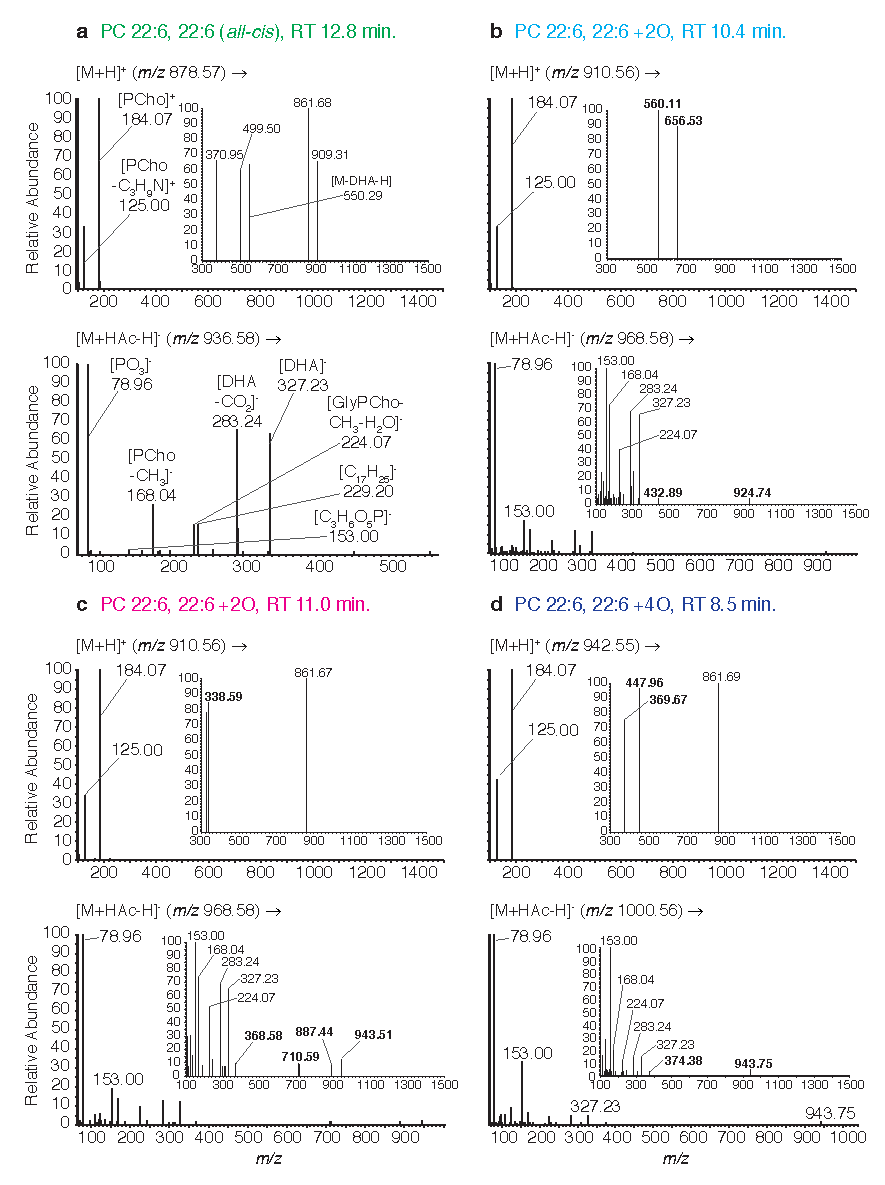
\includegraphics[width=1\textwidth]{Fig_4-9.pdf}
\end{figure}

We used the LOBSTAHS software and several other criteria (described in \autoref{sssec:Chap 4 - Identification and Quantification of Lipids and Oxidized Lipids}, above) to identify lipid degradation products in samples from the experiment presented in \autoref{fig:c4n6}. In the experiment, removal of the unoxidized PC 22:6, 22:6 molecule via photooxidation was accompanied by statistically significant rates of ingrowth of several unoxidized and oxidized derivatives (\autoref{fig:c4n7}, \autoref{fig:c4n8}a; \autoref{table:c4n1}). The former category included significant concentrations of lysophosphatidylcholine (LPC), while the latter included ox-PC species, oxylipins, and several ox-LPC species. The application of an unsupervised clustering algorithm to the data showed that changes in concentration in the various compounds were indicative of expected similarities between both treatments and timepoints (\autoref{fig:c4n7}). While the HPLC-MS data revealed several potential molecules of interest, we focused our efforts on a group of intact oxidized PC (ox-PC) species, a diverse class of molecules which have received increasing attention in human biomedicine (O'Donnell, 2011; Reis and Spickett, 2012; Spickett and Dever, 2005), some terrestrial plant studies (Vu et al., 2012), and other model systems (Ishida et al., 2004), but virtually no attention in oceanography or other avenues of environmental research. While research into the role of oxidized lipids has traditionally focused on the structural diversity and bioactivities of oxylipins --- the short-chain derivatives of fatty acids which are considered the ``terminal'' degradation products of lipid peroxidation processes (Andreou et al., 2009; Cutignano et al., 2011; G\"{o}bel and Feussner, 2009) --- an even broader potential structural and functional diversity exists among larger, more complex intact oxidized PC species and among other oxidized glycerophospholipids (L. T. Morgan et al., 2010; Spickett and Pitt, 2015).

\begin{figure} [!t]
\captionsetup{font={footnotesize}}
\captionof{figure}[Data-dependent MS\textsuperscript{2} spectra of PC 22:6, 22:6 and three oxidized degradation products]{(preceding page) Data-dependent MS\textsuperscript{2} spectra of (a) PC 22:6, 22:6 and (b)-(d) the three oxidized degradation products identified in the + UVB -- het. bact. sample presented in \autoref{fig:c4n8}. The top and bottom plots in each subpanel show, respectively, the positive and negative ionization mode fragmentation spectra for the major adduct of each analyte. Labeled features in (a) are the major ions diagnostic of the intact, unoxidized parent molecule; some of these are diagnostic PC headgroup fragments that also appear in (b)-(d). Boldface \emph{m/}z annotations in (b)-(d) indicate fragment ions unique to each oxidized species. Text colors used in column headings correspond to those used in \autoref{fig:c4n8} and \autoref{fig:aen4}. An expanded version of \autoref{fig:c4n9} is presented in \autoref{fig:aen4}.}
\label{fig:c4n9}
\end{figure}

Analysis of extracted ion chromatograms and data-dependent MS\textsuperscript{2} spectra allowed us to putatively identify a series of progressively more oxidized ox-PC species in a representative +UVB --het. bact. sample at the final experimental timepoint (\autoref{fig:c4n8}, \autoref{fig:c4n9}, and \autoref{fig:aen4}). The accuracy of our mass spectrometer and diagnostic headgroup fragments in the dd-MS\textsuperscript{2} spectra (\autoref{fig:c4n9} and \autoref{fig:aen4}) allowed us to first confirm the identities of these compounds at the level of chemical formula and lipid class. Consistent with the expected effect of increasing molecular polarity on retention time (RT) under reverse-phase chromatographic conditions (O'Donnell et al., 2009), we also observed a decrease in RT of each analyte in the series in proportion to the number of additional oxygen atoms it contained (\autoref{fig:c4n8}b-d; \autoref{table:c4n1}). Further increasing our confidence, an analogous relationship between RT and oxidation state was noted for each of the other types of oxidized species we identified (i.e., ox-LPC and the oxidized free fatty acid derivatives; \autoref{table:c4n1}).

Finally, unique ions observed the MS\textsuperscript{2} spectra for each putatively identified feature (\autoref{fig:c4n9}, S4) indicated either that (a) various positional isomers of each oxidized lipid were present, or (b) the exact nature of the oxidation was different in each case (e.g., the addition of two hydroxyl groups would yields ion of the same \emph{m/z} as one featuring a single hydroperoxy functional group). These unique fragments were distinguished from the common headgroup fragments characteristic of the PC lipid class and other fragments, such as those representing unoxidized DHA, which were present in nearly all of the species (\autoref{fig:c4n9}, S4). Based on previous findings (Milic et al., 2012; O'Donnell, 2011; Reis and Spickett, 2012; Sala et al., 2015; Spickett et al., 2011), we suspect that the apparent diversity of species within each oxidized lipid class reflects a combination of the two situations. We suspect that the compound, non-Gaussian peak shapes we observed for the PC 22:6, 22:6 +2O and PC 22:6, 22:6 +4O species (\autoref{fig:c4n8}c,d) indicate the presence of multiple, near-co-eluting ox-PC regioisomers (i.e., species with same oxidation state and type of oxidized functional group; Domingues et al., 2009; Reis et al., 2005). The presence of multiple isomers of each oxidized species in the sample is highly probable, given the multiple \emph{bis-}allylic positions in the parent molecule and the nonselective, abiotic origin of the peroxidation. Far fewer positional isomers are produced in the case of biologically mediated peroxidation of polyunsaturated fatty acids; this is because the lipoxygenase enzymes responsible for production of short-chain oxylipins tend to have high affinity for specific positions in the acyl chains of their target substrate (Andreou and Feussner, 2009; Brash, 1999; Cutignano et al., 2011; Feussner and Wasternack, 2002).

Because our choice of primary MS method did not yield fragmentation spectra for any of our analytes at levels \textgreater{} MS\textsuperscript{2}, we were unable to further characterize the structures of the ox-PC species we identified in our samples. While fragments diagnostic of specific oxidation types and positions are sometimes observed in the MS\textsuperscript{2} spectra of oxidized phospholipids, spectra obtained from successive fragmentation of target ions at levels \textgreater{} MS\textsuperscript{2} are needed to definitively resolve the structures of many ox-PC species. A significant and growing body of literature offers a wealth of information for analysis of MS\textsuperscript{3} and higher-level data obtained under a variety of HPLC-MS methods in both positive and negative ionization modes (Berliner et al., 2009; Buseman et al., 2006; Domingues et al., 2008; Ishida et al., 2004; Milic et al., 2012; L. T. Morgan et al., 2010; Ni et al., 2015; O'Donnell, 2011; Reis and Spickett, 2012; Sala et al., 2015; Spickett and Dever, 2005; Spickett et al., 2011; Thomas et al., 2010; Yin et al., 2009). Future work will extend the scope of this thesis by examining selected samples on an ion-trap instrument where MS\textsuperscript{n} fragmentation is possible. Authentic standards might also have been used to confirm the identities of some of the species in our samples, but (unlike their shorter-chain molecular cousins, the oxylipins) commercial standards do not exist for the vast majority of ox-PC species. Instead, standards must be obtained either through purification and concentration of fractions from natural samples, or by air oxidation of unoxidized IP-DAG, followed by SnCl\textsubscript{2} reduction and collection of fractions (A. H. Morgan et al., 2010); both of these methods are time-consuming and resource intensive, making the use of ox-PC standards within the scope of the present work prohibitive. The combination of methods we employed still allowed us to make putative identifications of our unknown analytes with a confidence falling somewhere between levels 2 and 3 in the proposed scheme of Sumner et al. (2007) for metabolite identification.

\subsection{Distributions and Acyl Saturation State of IP-DAG in Samples from Waters of the West Antarctic Peninsula}
\begin{figure}[!p]
\centering
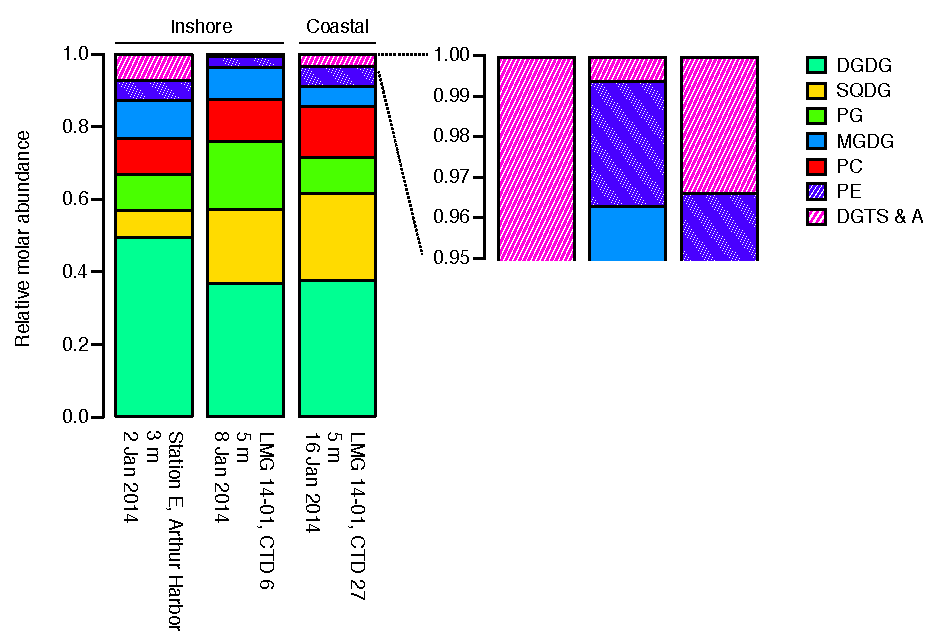
\includegraphics[width=1\textwidth]{Fig_4-10.pdf}
\captionsetup{font={footnotesize}}
\caption[Relative molar distribution of seven classes of IP-DAG in representative samples of particulate biomass from waters of the West Antarctic Peninsula]{Relative molar distribution of seven classes of intact polar diacylglycerol (IP-DAG) in representative samples of particulate biomass (fraction \textgreater{} 0.2 $\mu$m) from waters of the West Antarctic Peninsula. Samples were collected in 2014 from an inshore station (PAL-LTER Station E, 64.82$^{\circ}$ S, 064.055$^{\circ}$ W) and two coastal stations whose biogeochemistry was representative of oceanic influence (cruise LMG 14-01 CTDs 6 and 27, 64.88$^{\circ}$ S, 064.289$^{\circ}$ W and 68.159$^{\circ}$ S, 068.946$^{\circ}$ W, respectively; \autoref{fig:c4n1}). The CTD 6 (8 Jan) sample was obtained during a significant bloom event. Lipids were identified using the LOBSTAHS software (Collins et al., 2016) in conjunction with several additional criteria described in the text; 318 different compounds are represented in the figure. Quantification of lipids was performed using authentic standards. In addition to compounds in the seven lipid classes presented here, we identified several species of diacylglyceryl carboxyhydroxymethylcholine (DGCC) in the samples; these were excluded from the dataset used to generate the figure because we did not have a suitable authentic standard available at the time of analysis. DGCC accounted for \textless{} 11 \% of the total raw IP-DAG peak area in the Station E and CTD 27 samples, and 26.1 \% of the total IP-DAG peak area in the sample from CTD 6. The full, annotated list of the lipids identified in each culture is available online at \url{https://github.com/jamesrco/LipidPhotoOxBox/blob/master/data/nice/LOBSTAHS_lipid_identities/PAL1314_LMG1401_particulate_IP-DAG_pmol_L.final.csv} or upon request from the author.}
\label{fig:c4n10}
\end{figure}

After characterizing the diversity of PC species in HPLC-MS data from our liposome experiments, we applied the same strategy to identify the lipids present in five samples of particulate organic matter ($\geq$ 0.2 $\mu$m) collected from WAP surface waters during the austral spring of 2013-2014. Of the 4,393 different unoxidized and oxidized lipids we identified in the five samples, we used response factors determined from authentic standards to quantify 318 molecules in a subset that encompassed seven different classes of IP-DAG. Triacylglycerols (TAG) accounted for the vast majority (70.0 $\pm$ 8.8 \%, mean $\pm$ SD) of the total identifiable lipid peak area in the five samples. Results from three samples representative of different bloom conditions (\autoref{fig:c4n10} and \autoref{fig:c4n11}) indicated that species of the galactolipid DGDG, one of the four primary IP-DAG in the chloroplast membranes of photosynthetic organisms, accounted for the vast majority of the intact polar lipids we quantified in the data using authentic standards. Significant quantities of the sulfolipid SQDG and the phospholipids PC and PG were also present (\autoref{fig:c4n10}). A comparison of these results with profiles of IP-DAG in four diatom species isolated from WAP waters during the same season (\autoref{fig:aen5}) suggests that other taxa (e.g., heterotrophic bacteria or cryptomonads, which are becoming increasingly prevalent in WAP waters during the spring and summer; Ducklow et al., 2013; Montes-Hugo et al., 2009) contributed equally or more significantly to the surface ocean particulate lipid reservoir during the period. We also identified several oxidized lipid species in the water column samples; these included all of the intact oxidized degradation products of PC 22:6, 22:6 that had we observed in our liposome experiments. Features representing PC 22:6, 22:6 +1O (two obvious isomers), PC 22:6, 22:6 +2O, PC 22:6, 22:6 +3O, and PC 22:6, 22:6 +4O were detected at 7.2, 3.9, 5.1, 0.5, and 0.8 \%, respectively, of the abundance of PC 22:6, 22:6 (percentages are average values across the five samples; a full, annotated list of all identified compounds and their raw chromatographic peak areas are \href{https://github.com/jamesrco/LipidPhotoOxBox/tree/master/data/nice/LOBSTAHS_lipid_identities}{available online}).
\begin{figure}[!p]
\centering
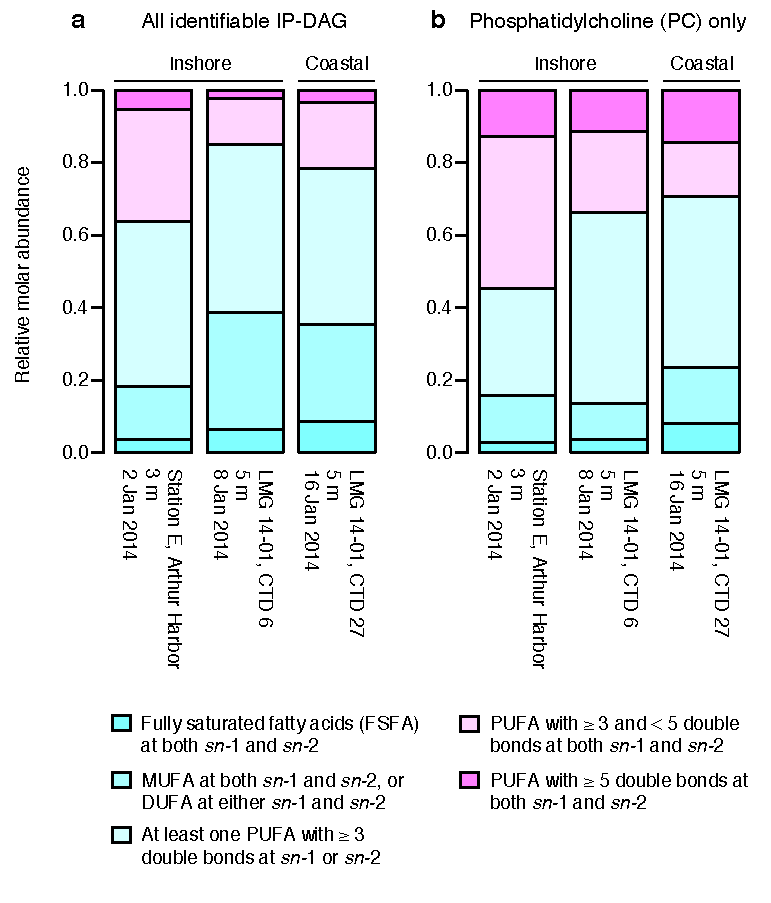
\includegraphics[width=.75\textwidth]{Fig_4-11.pdf}
\captionsetup{font={footnotesize}}
\caption[Fatty acid composition of IP-DAG in the sample presented in \autoref{fig:c4n10}]{Fatty acid composition of (a) all identifiable IP-DAG and (b) phosphatidylcholine (PC) species in the particulate biomass samples presented in \autoref{fig:c4n10}. Because the current version of the LOBSTAHS software resolves the identities of IP-DAG only to the level of bulk fatty acid composition (i.e., the sum of the properties of the substituents at both the \emph{sn}-1 and \emph{sn}-2 positions), we were unable to determine which fatty acids were present in each molecule without significant additional inspection of fragmentation spectra or saponification for analysis of fatty acid methyl esters (FAMES). However, we were able to categorize the saturation state of the IP-DAG according to the simplified scheme we present here after verifying (by inspection of fragmentation spectra) that the maximum degree of unsaturation of any single fatty acid present in these species was six (present in the form of docosahexaenoic acid, or DHA).}
\label{fig:c4n11}
\end{figure}

As a second means of analysis with direct relevance to the project described in this chapter, we binned the IP-DAG species in each water column sample into five categories based on the saturation state of their attached fatty acids (\autoref{fig:c4n11}). Molecular species containing highly polyunsaturated fatty acids (i.e., those with $\geq$ 5 double bonds) at both substituent positions accounted for 5.3, 2.3, and 3.4 \% of the IP-DAG in samples from PAL-LTER Station E and LMG 14-01 CTD stations 6 and 27, respectively (percentages calculated on basis of molar concentration; \autoref{fig:c4n11}a). Lipids containing two fatty acids of moderate polyunsaturation (i.e., $\geq$ 3 but \textless{} 5 double bonds) accounted for 31.1, 12.7, and 18.2 \% of IP-DAG in the three samples. When we examined the acyl saturation state of molecular species belonging to single classes of IP-DAG, it became apparent that PUFA were not evenly distributed throughout the WAP metalipidome (e.g., PUFA were concentrated more heavily in species of PC than in the IP-DAG pool as a whole; \autoref{fig:c4n11}b). Comparison of these results with a similar analysis of fatty acid distribution among IP-DAG classes in the four diatom isolates (\autoref{fig:aen6}) again showed that the lipids of these diatoms did not dictate the composition of the overall WAP lipid pool, despite these species being traditionally responsible for most early-season blooms in WAP waters.

\section{Discussion}
\subsection{Apparent Dependence of Photolability on Acyl Polyunsaturation}
\label{ssec:Apparent Dependence of Photolability on Acyl Polyunsaturation}

PC 22:6, 22:6 was the only species we evaluated that contained polyunsaturated fatty acids (PUFA) with more than two double bonds (\autoref{table:aen1}; molecular structures, \autoref{fig:aen1}). Our laboratory measurements of decadic molar absorptivity show that the capacity of PC 22:6, 22:6 to absorb light in both the UVB and UVA spectral bands exceeded by nearly two orders of magnitude those of direct molecular analogs containing fully saturated (PC 22:0, 22:0) and monounsaturated (PC 22:1, 22:1) fatty acids of the same chain length (\autoref{fig:c4n5}c). The large difference we observed between the molar absorptivity of the hexa-unsaturated compound and its more saturated analogs was corroborated by similar results previously reported for other sequences of related phospholipids (McHowat et al., 1996; Spector et al., 1996). In addition, UV-visible absorbance measurements of docosahexaenoic acid, the constituent fatty acid of PC 22:6, 22:6, indicated that the parent molecule's light-absorbing capacity was due primarily to the presence of the highly unsaturated acyl moiety and not the polar headgroup (\autoref{fig:c4n5}b,c). Absorbance measurements of the lipid standards were repeated for verification in three independent experiments over the course of two months. While no molar absorptivity data have been published for PC 22:6, 22:6, the ${\varepsilon _i}(\lambda )$ we calculated for DHA agreed generally with values found in the literature (Whitcutt, 1957). In the only investigation directly analogous to the work in this thesis chapter, R. J. Kieber et al. (1997) investigated the photochemical reactivity of highly polyunsaturated free fatty acids in seawater under exposure to natural sunlight. In that study, photodegradation rates of C\textsubscript{16} and C\textsubscript{18} PUFA were nearly 10 times those of the species' monounsaturated counterparts and --- perhaps most instructively for purposes of interpreting the present results --- the investigators observed almost no photodegradation in the saturated member of the C\textsubscript{16} series, palmitic acid. Rontani et al. (1998) observed a similar trend for a series of C\textsubscript{18:1}-C\textsubscript{18:3} fatty acids isolated from algal cultures; while that experiment did not include any PUFA with more than three double bonds, the degradation rate constant the authors observed for the C\textsubscript{18:3} species was more than six times that observed for C\textsubscript{18:1}.

While Wagner et al. (1994) did not specifically investigate the \emph{photochemical} lability of fatty acids, they hypothesized that the ``oxidizability'' of a given PUFA --- the overall susceptibility of its hydrogen atoms to abstraction by radical species such as $\bullet$OH --- was proportional not simply to the number of double bonds in the fatty acid, but to the number of \emph{bis-}allylic positions in the fatty acid chain. Applying this hypothesis in a series of experiments, the authors found that the addition of each new double bond which created a \emph{bis-}allylic carbon atom increased exponentially the rate at which a given fatty acid was oxidized. The bond dissociation energy of a doubly allylic C-H bond was reported to be just 314-335 kJ mol\textsuperscript{-1}, compared with 368 kJ mol\textsuperscript{-1} for a singly allylic bond and 423 kJ mol\textsuperscript{-1} for an alkyl C-H bond (Gardner, 1989; Koppenol, 1990).

\subsubsection{Other Sources of Evidence for Preferential Photooxidation of PUFA-Containing Lipids}

Beyond the previous results we reviewed in in the above paragraphs (\autoref{ssec:Apparent Dependence of Photolability on Acyl Polyunsaturation}), we could find no empirical evidence in the literature for a quantitative relationship between IP-DAG molecular structure (specifically, the degree of acyl unsaturation) and photochemical lability in the environment or under environmentally relevant experimental conditions. Several lines of evidence generally substantiate the enhanced photochemical lability of acyl lipids bearing polyunsaturated fatty acids over closely related molecules with lower degrees of unsaturation. First, an extensive body of research spanning diverse scientific disciplines has long ranked polyunsaturated fatty acids among the cellular lipid components most susceptible to photooxidation (Girotti, 1990; Heath and Packer, 1968; Rontani, 1999) and transformation by reactive oxygen species (ROS) generally (Frankel, 1980; 1987; Girotti, 1998; Li and Schwarz, 2012; Mene-Saffrane et al., 2009). Some evidence for a quantitative relationship between acyl unsaturation and photochemical lability in IP-DAG exists in human biomedicine, where artificial near-IR radiation can be used to trigger release of pharmaceutical compounds from liposomes for targeted, intracellular drug delivery. In one study that investigated the intracellular release of a cancer chemotherapy medication encapsulated in PC liposomes, a quantitative, negative relationship was observed between the degree of unsaturation of the fatty acids used in the liposomes and the time required to achieve 50 \% release of the drug into the cell (Luo et al., 2016). Earlier work (Pashkovskaya et al., 2010) suggested the mere presence of unsaturated acyl moieties could dramatically enhance the apparent photochemical lability of the entire liposome pool used for drug delivery, a finding consistent with evidence that autooxidation of saturated lipid moieties can be initiated by lipid radicals derived from oxidation of nearby PUFA (Girotti, 1998).

Of course, there is abundant evidence from incubation experiments with both single-species cultures and whole communities of phytoplankton that PUFA are preferentially underexpressed in marine microorganisms that are subjected to high doses of UV radiation (Hessen et al., 1997). Whether this is predominantly because cell membranes containing these PUFA are abiotically oxidized at a greater rate under UV radiation, or because UV radiation inhibits the organisms' ability to synthesize these critical compounds is not clear; both mechanisms appear to be important (Goes et al., 1994). Hessen et al. (1997) and Wang and Chai (1994) both noted that phytoplankton membrane lipids containing eicosapentaenoic acid (EPA, 20:5$\omega$3) and DHA were particularly susceptible to photooxidation, confirming our results in the present study (\autoref{fig:c4n6}a; \autoref{table:c4n1} and \autoref{table:aen1}); Wang and Chai found that an acute dose of strong UVB radiation elicited a stronger response than application of a less intense dose over a longer time period. After exposing cultures of three Antarctic marine phytoplankton to different levels of UVB radiation, Skerratt et al. (1998) found some evidence that UVB exposure could reduce intercellular ratios of unsaturated to saturated fatty acids; however, the response to UVB exposure was species-specific and depended heavily on the dosage. For example, while the ratio of PUFA : FSFA remained virtually unchanged in the diatom \emph{Odontella weissflogii} after two days of exposure to elevated concentrations of UVB radiation, the percentage of total fatty acids identified as PUFA in the diatom \emph{Chaetoceros simplex} decreased from 37 to 31 \%. Guih\'{e}neuf et al. (2010) also noted that the response of different phytoplankton species to UVB radiation appeared highly species specific, observing significant reductions in EPA and DHA-containing phospho- and glycolipids in one species (\emph{Pavlova lutheri}) yet very little change in another (\emph{Odontella aurita}).

\subsection{Possible Mechanisms Supporting Observed Rates of Photooxidation}

Although the original scope of this chapter did not extend to identification of the mechanism(s) responsible for the photooxidation we observed in the liposome experiments, several conclusions can be drawn from synthesis of available environmental and optical data, the results of two \emph{ad hoc} experiments, and previous findings regarding photochemical processes in waters of the WAP and other polar marine ecosystems. First, our results show that photooxidation could have been supported by both indirect (i.e., via ROS produced through reactions with chromophoric substances) and direct (i.e., via the action of a photon directly upon a molecule) processes. We observed penetration through nearly the entire mixed layer (see \autoref{ssec:Irradiance Observations; UV Penetration Through Shallow Mixed Layer}, above) of significant radiation in both the UVA and UVB spectral bands, indicating ample photons were available in the surface water column to initiate or catalyze a variety of reactions; nearly 70 \% of incident UVB radiation (\autoref{fig:c4n3}a and \autoref{fig:c4n4}) and 40 \% of UVA radiation (\autoref{fig:c4n3}b and \autoref{fig:c4n4}) were observed to reach a depth of 0.6 m. Based on the abundance of UVA radiation in the water column and the 314-335 kJ mol\textsuperscript{-1} bond energy previously reported for the doubly allylic C-H bonds in model PUFA (Gardner, 1989; Koppenol, 1990), we suggest direct photolysis of PC 22:6, 22:6 could have contributed significantly to overall rates of PUFA photooxidation throughout much of the shallow surface layer. The 314-335 kJ mol\textsuperscript{-1} bond energy is equivalent to that carried by UVA-band photons of $\lambda$ between 357 and 381 nm; quanta of this energy were abundant to depths of at least 8 m in the waters of Arthur Harbor (\autoref{fig:c4n4}).

Of the many possible indirect mechanisms that could have supplemented direct photolysis in immediate surface waters during the period of our study, the generation (and peroxidation thereby) of hydroxyl radical from photoexcitation of existing nitrate and nitrite stocks was almost certainly significant. Qian et al. (2001) found that UVA + UVB excitation of DOM, combined with UVB excitation of relatively high NO\textsubscript{3}\textsuperscript{-} concentrations often typical of Southern Ocean waters, led to enhanced rates of $\bullet$OH production in surface waters of the WAP. While we did not measure production rates or steady-state concentrations of $\bullet$OH in the present study, the daily doses of UVB radiation received at Palmer Station in the spring of 2013 were similar to those received on many days during the season in which Qian et al. conducted their study. Furthermore, in 2013-2014, surface concentrations of NO\textsubscript{3}\textsuperscript{-} + NO\textsubscript{2}\textsuperscript{-} remained at or above 15 $\mu$M at PAL-LTER Stations B and E until early January, providing a sufficient reservoir of the chromophore to sustain production of hydroxyl radical at biogeochemically significant rates (public PAL-LTER data; not shown). While a combined concentration of the two nutrients of just 1.2 $\mu$M was measured at Station E following a bloom event in mid-January, concentrations at both stations increased again soon after the event to yield a seasonal average of 15.0 $\mu$M at depths \textless{} 5 m. The ability of $\bullet$OH to abstract hydrogen atoms from PUFA has been well-demonstrated (Porter et al., 1995; Wagner et al., 1994) and we therefore do not devote additional discussion to the topic here.

While photochemical generation of other ROS such as \textsuperscript{1}O\textsubscript{2}, H\textsubscript{2}O\textsubscript{2}, and O\textsubscript{2}\textsuperscript{-} might certainly have augmented the two photochemical sinks we discuss in the paragraph above, we believe it unlikely that photochemically produced H\textsubscript{2}O\textsubscript{2} and O\textsubscript{2}\textsuperscript{-} contributed significantly to overall rates of lipid degradation in our experiments. Photoexcitation in the laboratory of previously frozen, 0.7 $\mu$m-filtered water samples from Arthur Harbor (the experiments described in \autoref{ssec:Laboratory Determination of ROS Photoproduction and Decay}) yielded negative results at all wavelengths; photoproduction rates of H\textsubscript{2}O\textsubscript{2} and O\textsubscript{2}\textsuperscript{-} remained below detection in all instances. We still could not detect any superoxide after spiking the sample with 10-200 nM KO\textsubscript{2}; this suggested the seawater contained a strong abiotic quenching agent capable of scavenging the two ROS. However, the outcome of this brief experiment is challenged by the findings of both Yocis et al. (2000), who measured H\textsubscript{2}O\textsubscript{2} photoproduction rates of 2.1 to 9.6 nM H\textsubscript{2}O\textsubscript{2} hr\textsuperscript{-1} in fresh, unfiltered West Antarctic waters, and of Kieber et al. (2014), who made similar findings. Thus, a biological source of H\textsubscript{2}O\textsubscript{2} might have contributed to rates of lipid oxidation in natural waters outside of our experimental construct; water column concentrations of 10-100 nM H\textsubscript{2}O\textsubscript{2} were observed at Palmer Station during the 2015-2016 field season (although, H\textsubscript{2}O\textsubscript{2} concentrations in dense algal biomass were as high as 200 nM; J. Bowman, \emph{Pers. comm.}). The 2015-2016 water column concentrations were consistent with the concentrations measured in surface waters at several offshore PAL-LTER stations during the early 1990s (12-21 nM; Resing et al., 1993). We did not make measurements of singlet oxygen in the course of this work, and it is likely the species contributed significantly to the rates of photooxidation we report here. Type II (i.e., \textsuperscript{1}O\textsubscript{2}-mediated) photooxidation of lipids has been proposed as the dominant pathway for photooxidation in marine systems of monounsaturated fatty acids and photosynthetic pigments (Rontani, 1999)

\subsection{Biogeochemical Significance of Lipid Photooxidation in Surface Waters of the West Antarctic Peninsula}
\subsubsection{Choice of Apparent Quantum Yield for Use in Calculations}

Using the oxidation rates we obtained from our liposome experiments and several other measured properties, we calculated three broadband polychromatic AQY for photooxidation of PUFA-containing IP-DAG in coastal waters of West Antarctica (\autoref{table:c4n2}). Uncertainities were determined as described in \autoref{sssec:Determination of Uncertainties in AQY Estimates}. Based on our findings that UVB radiation did not significantly enhance rates of photooxidation in PUFA-containing IP-DAG beyond those rates observed in the presence of UVA radiation alone (\autoref{fig:c4n6}; \autoref{table:c4n1}), we chose to apply in our subsequent calculations the broadband AQY ${\Phi _{UVA}}$, which parameterizes the photooxidation rate as a function of the total radiation received in the UVA spectral band. Our laboratory measurements confirmed the capacity of PC 22:6, 22:6 to absorb light over a broad wavelength range that extended far into the UVA spectrum (\autoref{fig:c4n5}). Because we could find no AQY (polychromatic or otherwise) in the literature for IP-DAG or polyunsaturated fatty acids, the best empirical evidence outside the present study comes from the rate constants calculated by Christodoulou et al. (2010), Rontani et al. (1998), and others. In applying a yield that accounts for multiple processes operating across a wide spectrum, we proceed from the conclusion of the former authors, who found that maximum degradation rates of polyunsaturated lipids in senescent phytoplanktonic cells were induced by both a combination of visible light (photosynthetically active radiation wavelengths) and UVA radiation. To obtain a conservative estimate of the possible impact of lipid photooxidation on the organic matter inventory in surface waters of the West Antarctic Peninsula, we applied our broadband AQY to the most polyunsaturated fraction of the IP-DAG identified in our water column samples (\autoref{fig:c4n11}). For comparison, we made a series of parallel calculations in which we applied the same AQY to the larger, moderately polyunsaturated fraction of the IP-DAG inventory. We assumed in our calculations that the residence times of suspended and slowly sinking particulate organic matter in the mixed layer were long (i.e., on timescales of days) compared with the timescale over which photodegradation was observed to act in our liposome experiments (i.e., 8.2-12.4 hr).
\begin{figure}[!p]
\centering
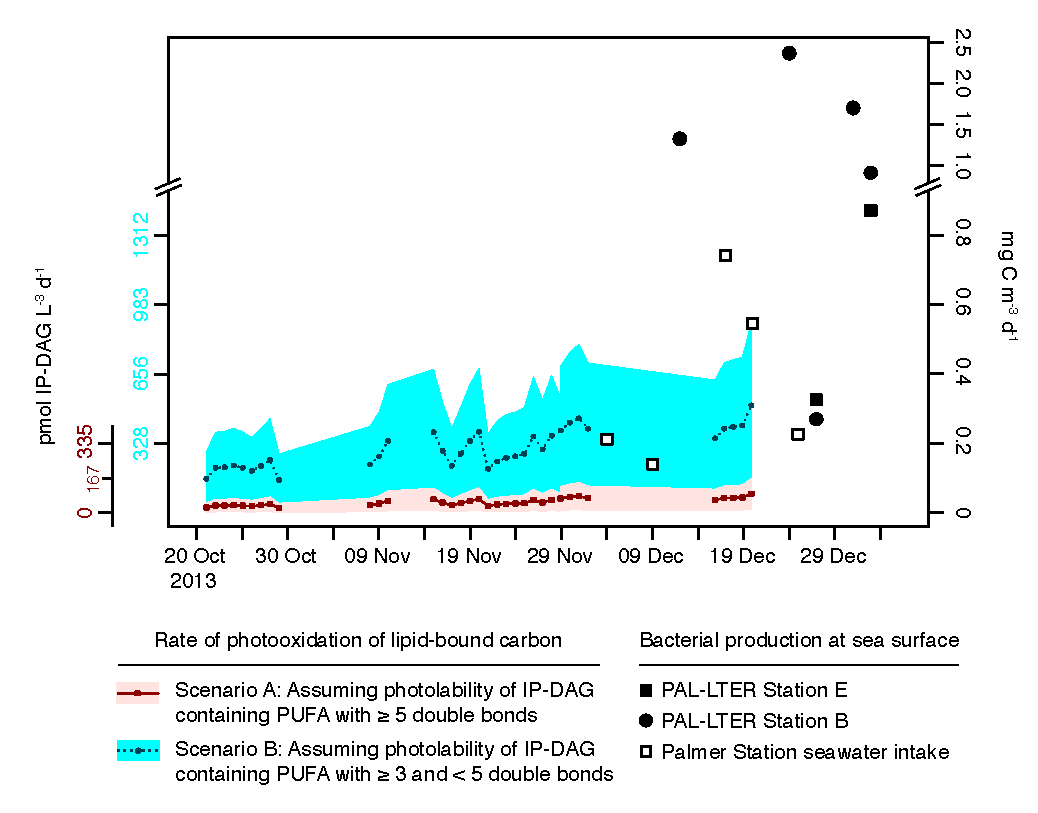
\includegraphics[width=1\textwidth]{Fig_4-12.pdf}
\captionsetup{font={footnotesize}}
\caption[Potential rates of lipid photooxidation in particulate organic matter of West Antarctic Peninsula surface waters]{Potential rates of lipid photooxidation in particulate organic matter of West Antarctic Peninsula surface waters over a 2-month period in the austral spring of 2013. High-resolution, \emph{in situ} time-series observations of downwelling irradiance and a broadband polychromatic apparent quantum yield (AQY) for IP-DAG species containing highly polyunsaturated fatty acids (${\Phi _{UVA}}$) were applied to separate fractions of lipids identified using the LOBSTAHS software to generate two sets of photooxidation rate estimates. In the first, most conservative scenario (red markers and solid trace), we applied the irradiance time series and AQY to only those IP-DAG containing PUFA with $\geq$ 5 double bonds at both the \emph{sn}-1 and \emph{sn}-2 backbone positions. In the second, more permissive scenario (cyan markers and dashed trace), we assumed the AQY could also be applied to molecular species containing PUFA with $\geq$ 3 but \textless{} 5 double bonds. ${\Phi _{UVA}}$ represents the reaction yield for lipid photooxidation based on the quantity of UV radiation received between 315 to 395.5 nm; estimation of ${\Phi _{UVA}}$ and the associated uncertainty is described in \autoref{ssec:Calculation of Broadband Polychromatic Apparent Quantum Yields (AQY)} of the text. The shaded regions represented the propagated uncertainties in each estimate determined using a series of Monte Carlo simulations. Lipid photooxidation rates (left-hand \emph{y-}axis) were converted units of mg C m\textsuperscript{-3} d\textsuperscript{-1} based on the mean carbon content of the IP-DAG identified in each unsaturation fraction; these were 49.3 $\pm$ 0.5 and 50.6 $\pm$ 0.6 mol C : mol lipid for the polyunsaturated (cyan) and highly polyunsaturated (red) fractions, respectively. Presented for comparison are volumetric rates of bacterial production for West Antarctic Peninsula surface waters, obtained using the \textsuperscript{3}H-leucine incorporation method (large individual symbols, from PAL-LTER data; Bowman et al., 2016). Note the break and change in scale of the \emph{y-}axis.}
\label{fig:c4n12}
\end{figure}
\subsubsection{Photooxidation Rates in Austral Spring of Same Order of Magnitude as Bacterial Production}

Our results (\autoref{fig:c4n12}) suggest that photooxidation of IP-DAG containing highly polyunsaturated fatty acids represents a biogeochemically significant process in this ecosystem of a magnitude commensurate with that of bacterial production. While limiting the scope of our findings to the early spring --- when nearly all of the suspended particulate biomass in the shallow mixed layer receives enhanced doses of UV radiation through a depleted stratospheric ozone layer --- we estimate conservatively that, on average, 50 $\pm$ 11 pmol IP-DAG L\textsuperscript{-1} d\textsuperscript{-1} was oxidized in the mixed layer by photochemical processes (this is the equivalent of 0.031 $\pm$ 0.007 mg C m\textsuperscript{-3} d\textsuperscript{-1}; \autoref{fig:c4n12}, red markers and solid red trace). Under the second, less conservative scenario --- in which we applied the AQY to a larger subset of the IP-DAG inventory --- we estimate that roughly 6 times this quantity of lipid organic matter was potentially oxidized through photochemical mechanisms (295 $\pm$ 66 pmol IP-DAG L\textsuperscript{-1} d\textsuperscript{-1}, equivalent to 0.17 $\pm$ 0.04 mg C m\textsuperscript{-3} d\textsuperscript{-1}; \autoref{fig:c4n12}, cyan markers and dashed trace). For comparison, average surface ($\leq$ 5 m) rates of bacterial production at the three PAL-LTER stations in the period before 4 January 2014 were 0.38 $\pm$ 0.26, 1.3 $\pm$ 0.8, and 0.60 $\pm$ 0.4 mg C m\textsuperscript{-3} d\textsuperscript{-1} (Palmer Station seawater intake, PAL-LTER Station B, and PAL-LTER Station E, respectively, assuming a conversion factor of 1.5 kg C (mol leucine)\textsuperscript{-1} and isotope dilution of 1; \autoref{fig:c4n12}, larger symbols). We thus calculate that, during the early spring, lipid photooxidation might represent a flux of between 2-8 \% (conservative scenario) or 13-45 \% (alternative scenario) of the strength of bacterial carbon metabolism in WAP surface waters. We suspect that even our less conservative calculations might still represent an underestimate of the overall significance of lipid photooxidation in WAP waters because we did not apply our model to any fraction of the lipid biomass allocated to triacylglycerols, which accounted for 70-75 \% of the total identifiable chromatographic peak area in the water column samples. Although the AQY was derived from photooxidation experiments in PC, we justify its application to other classes of IP-DAG on the basis of evidence (from human systems) that changes in headgroup do not dramatically affect \emph{in situ} oxidation rates so long as the attached PUFA are of high unsaturation (Reis and Spickett, 2012).

We converted our photooxidation rate estimates from units of lipid (i.e., pmol IP-DAG m\textsuperscript{-3} d\textsuperscript{-1}) to carbon based on the carbon content of the IP-DAG identified in each unsaturation fraction; these were 49. 3 $\pm$ 0.5 and 50.6 $\pm$ 0.6 mol C : mol lipid for the polyunsaturated (cyan) and highly polyunsaturated (red) fractions, respectively. In doing so, we assumed that photooxidation of given lipid would in most instances lead to the eventual remineralization of the molecule's constituent carbon. Because lipid peroxidation proceeds by a free radical chain reaction mechanism (Girotti, 1990; Halliwell and Chirico, 1993), we assumed that, in the environment, the vast majority of initial oxidation products --- such as the ox-PC we have identified in this study --- would further degrade into smaller molecular components, while also initiating the degradation of other nearby lipids (and other molecules) that contain easily abstracted hydrogen atoms (Crastes de Paulet et al., 1988). The significant fraction of these smaller molecules that enter the dissolved organic matter pool will remain near the ocean's surface where, as previous work has demonstrated, they may be oxidized abiotically to dissolved inorganic carbon (Miller and Zepp, 1995). Equally as likely, these smaller, more labile molecules may be assimilated and remineralized by heterotrophic bacteria in the water column; this fate is support by considerable previous work (reviewed in D. J. Kieber, 2000) and our findings in \autoref{sssec:Some Support for Bacterial Metabolism of Oxidized Degradation Products}. However, we acknowledge here the many adaptations to oxidative stress possessed by phytoplankton, including considerable capacity to dissipate ROS and dozens of mechanisms for repair of damage to oxidized biomolecules (Roy, 2000). It is thus possible, as Rontani et al. (2016) have suggested based on observations in the Arctic, that the lipids in living phytoplankton cells may be much less susceptible to photooxidation than lipids in senescent or dead biomass. We do note that in the 2016 study, Rontani et al. did not look for evidence of photooxidation in intact lipids (i.e., ox-IPL) or in the oxidized products of lipids containing fatty acids with more than one double bond.

Our results nevertheless suggest that the shallow mixed layers which can form in the marginal ice zone provide a sort of ``optical incubator'' for UVR-induced lipid peroxidation in the WAP. In this model, particulate organic matter, including both ice-attached and free-living phytoplankton and bacteria, is exposed for extended periods to intense UV radiation at the immediate sea surface, increasing photooxidation rates of photolabile compounds such as PUFA-containing IP-DAG. Rontani et al. (2016) applied a version of this model to a recent analysis of lipid biomarkers in surface-layer biomass and shallowly deployed sediment traps (5 and 30 m) at the MIZ in the Canadian Arctic, finding that extended exposure to UVR of slowly-sinking aggregates derived from senescent sea-ice algae left a strong imprint on the photodegradation state of the lipid pool.

\subsection{Future Implications for the West Antarctic Peninsula Marine Ecosystem}

Three significant, relatively recent changes in the ecosystem of the West Antarctic Peninsula (Ducklow et al., 2013; Saba et al., 2014) make it difficult to predict how (or whether) lipid photooxidation will impact rates of primary production or carbon export in the future. First, shifts in the species composition of the phytoplankton community responsible for primary production in waters of the West Antarctic Peninsula --- particularly, increases in the prevalence of cryptophytes (or cryptomonads; phytoplankton of the phylum Cryptophyta) at the expense of the diatoms traditionally responsible for most of the carbon fixation (Montes-Hugo et al., 2009) --- will likely drive shifts in the lipid composition of surface ocean biomass during and after the annual retreat of the sea ice. While much is known about the lipid profiles of diatoms generally and species native to Antarctica in particular (e.g., \autoref{fig:aen5} and \autoref{fig:aen6}), relatively little comparable data exists for cryptophytes, apart from a few select species which have been investigated extensively for their potential as a feedstock for biodiesel production. DGDG is the most abundant IP-DAG in at least one cryptophyte, \emph{Chroomonas salina} (Henderson and Mackinlay, 1989).

Second, should the significant warming of WAP waters that has been observed in recent decades continue (Ducklow et al., 2013), the increase in average sea surface temperature could drive changes in the saturation state of the marine lipid pool independent of any change attributable to shifts in species distribution. Experimental results in cultures of several different marine phytoplankton species show that even modest increases in temperature can drive significant decreases in the proportion of overall membrane lipids that contain polyunsaturated fatty acids (Guschina and Harwood, 2006). This general relationship between saturation state and temperature has been demonstrated specifically in cultures of \emph{C. salina} (Henderson and Mackinlay, 1989). While the lipid inventories at several sites along the West Antarctic Peninsula presently include robust concentrations of IP-DAG with sufficient PUFA to support biogeochemically significant rates of photooxidation (\autoref{fig:c4n11} and \autoref{fig:c4n12}), warmer waters and an ecological shift toward phytoplankton species of largely uncharacterized lipid composition could alter the significance of photooxidation in the ecosystem.

Third, reductions in the duration and extent of sea ice cover that have accompanied the increase in WAP sea surface temperatures (Meredith and King, 2005) will likely diminish the strength of ice-associated and ice-attached diatom communities and their relative contribution to the overall lipid pool. The lipids produced by ice-attached diatom communities are different in many ways from those produced by diatoms which make their living in the water column (Fahl and Kattner, 1993; Falk-Petersen et al., 1998; Mock and Kroon, 2002). Because primary production in WAP waters is typically distinguished by bloom events that begin at the receding sea ice edge in spring or early summer (Ducklow et al., 2013; Vernet et al., 2008), warming water and concomitant changes in annual sea-ice dynamics could also advance the timing of blooms to earlier in spring and shift their locations further south, which could lead to ever greater temporal and spatial coincidence between maximum UVR exposure and peak phytoplankton abundances. A final, more recent trend --- the reduction in the size of and severity of the seasonal ozone anomaly over Antarctica, driven by recovery in stratospheric O\textsubscript{3} stocks (Solomon et al., 2016) --- could represent a significant negative feedback on photooxidation, further complicating any attempt to predict the overall significance of the process in a future ecosystem state.

\section{Conclusions and Additional Biogeochemical Implications}

While we show here that lipid photooxidation is a biogeochemically significant process that can impact the turnover of carbon in the surface ocean on scales commensurate with bacterial remineralization, it was ultimately beyond the scope of this thesis to determine whether the photooxidation of lipids containing polyunsaturated fatty acids leaves any significant imprint on the quality or the magnitude of organic matter exported to the ocean's depths. While we did not observe statistically significant rates of photooxidation in monounsaturated IP-DAG, a significant body of literature has shown that MUFA-derived oxylipins (i.e., free fatty acid derivatives cleaved from their lipid headgroup) do contribute to the oxidized lipid pool in surface waters, sinking particles, and seafloor marine sediments on scales which are all environmentally relevant (Marchand and Rontani, 2001; Rontani, 1999; Rontani et al., 2016; Rontani et al., 2012a; Rontani et al., 2012b). In Antarctic waters specifically, there is reason to presume that oxidation and removal of certain lipids at the ocean's surface could affect the quality of the lipid biomass that is exported to depth. Hayakawa et al. (1996) used a moored sediment trap at a site in Breid Bay, East Antarctica (trap depth 111 m; water depth 300 m) to examine the fatty acid content of sinking particles at 3.5-day intervals over three months, finding that the composition of the material bore the direct imprint of biogeochemical events at the ocean's surface. PUFA accounted for an average of 8.6 \% of fatty acids in all samples collected over the course of the study, but \textgreater{} 16 \% of the total during two diatom blooms which were observed at the site in the austral spring. EPA (20:5$\omega$3) alone accounted for 7.3 and 9.1 \% of the total during the two bloom events. Of course, one must also consider the possible impact that UV-induced PUFA photooxidation (and/or suppression of PUFA biosynthesis) in living phytoplankton might have for grazing zooplankton and, in turn, higher trophic level consumers. Ha et al. (2014) found that experimentally-induced reductions in the PUFA quotient of lipids in a sub-Antarctic natural phytoplankton assemblage --- particularly, reductions in the concentrations of DHA and EPA --- were passed in part to amphipods that fed on the phytoplankton deficient in essential fatty acids.

Finally, this study does not even begin to address the diversity of possible infochemical impacts that the many new oxidized phospholipid compounds we putatively identify (\autoref{fig:c4n7}, \autoref{fig:c4n8}, \autoref{fig:c4n9}, and \autoref{fig:aen4}) might have on intracellular processes, interactions between microoorganisms in the water column, or on the remineralization of sinking marine particles. Edwards et al. (2015) demonstrated the significant impact that modest concentrations of a single class of well-characterized oxylipin could have on the rate at which sinking marine particles were remineralized; given the hundreds of other oxylipins and many different intact oxidized phospholipids with significant known or hypothesized bioactivities in humans (Reis and Spickett, 2012; Spickett and Dever, 2005; Spickett and Pitt, 2015) and terrestrial plants (Vu et al., 2012), it is highly probable that some of these same compounds or their close analogs must play similar or as-yet-unimagined roles in the ocean.

\section{Acknowledgements}

We thank the captains, crew, and science support staff of the ARSV \emph{Laurence M. Gould}, the science support staff at Palmer Station during the 2013-2014 and 2015-2016 field seasons, and many current and former PAL-LTER team members for assistance with field sampling and sample analysis. We thank Jeff Bowman, Ollie Zafiriou, and Collin Ward for various discussions that focused our hypotheses and sampling plan. We also thank Kevin Becker, Peter Blandori, Nicole Couto, Julia Diaz, Scott Doney, Bethanie Edwards, Matthew Erickson, Tina Haskins, Meredith Helfrich, Oliver Ho, Fiona Hopewell, Carolyn Lipke, Austin Melillo, Justin Ossolinski, Naomi Shelton, Jeremy Tagliaferre, and Sebastian Vivancos for various analytical and logistical assistance. Oligotrophic seawater from the BATS site was kindly provided by Dan Repeta. Assistance with data from the Antarctic Ultraviolet Monitoring Network was provided by Patrick Disterhoft and the radiation group of NOAA's Global Monitoring Division, 325 Broadway, Boulder, CO, 80303. J.R.C. acknowledges support from a U.S. Environmental Protection Agency (EPA) STAR Graduate Fellowship (Fellowship Assistance agreement FP-91744301-0). The contents of this research have not been formally reviewed by EPA. The views expressed in this manuscript are solely those of the authors, and EPA does not endorse any products or commercial services mentioned therein. This work was also supported by U.S. National Science Foundation award OCE-1059884 to B.A.S.V.M., the Gordon and Betty Moore Foundation through grant GBMF3301 to B.A.S.V.M., and a WHOI Ocean Ventures Fund award to J.R.C. The field work conducted at Palmer Station and aboard the ARSV \emph{Laurence M. Gould} was supported by the Palmer LTER study (U.S. NSF awards OPP-9011927, 9632763, 0217282, 0823101, and GEO-PLR 1440435).

\section{Availability of Data, Code, and Supplementary Methodological Details}

The R scripts and processed data files required to reproduce the results and figures in this work are available online at \url{https://github.com/jamesrco/LipidPhotoOxBox}. Methodological details, additional figures, and an additional table, are included as supporting information. All PAL-LTER data used in this manuscript were downloaded from the Palmer LTER Datazoo at \url{http://oceaninformatics.ucsd.edu/datazoo/data/pallter/datasets}. Raw MS data files (\textgreater{} 200 MB) and raw spectral data collected using the Jaz instrument are available upon request from the author. Processed MS data, aggregated Jaz spectra, and detailed protocols for liposome preparation and the exoenzyme assays are available via the GitHub link above. NOAA spectroradiometer data were downloaded from \url{http://www.esrl.noaa.gov/gmd/grad/antuvdata/}.
\clearpage
\begin{singlespace}
\section*{References}
\addtocounter{section}{1}
{\setlength{\parindent}{0pt}
Andreou, A., and I. Feussner (2009), Lipoxygenases - Structure and reaction mechanism, \emph{Phytochemistry}, \emph{70}(13-14), 1504-1510, doi:\href{http://dx.doi.org/10.1016/J.Phytochem.2009.05.008}{10.1016/J.Phytochem.2009.05.008}.

{\setlength{\parskip}{10pt}

Andreou, A., F. Brodhun, and I. Feussner (2009), Biosynthesis of oxylipins in non-mammals, \emph{Progress in Lipid Research}, \emph{48}(3-4), 148-170, doi:\href{http://dx.doi.org/10.1016/J.Plipres.2009.02.002}{10.1016/J.Plipres.2009.02.002}.

Armstrong, D., and R. Browne (1994), The analysis of free radicals, lipid peroxides, antioxidant enzymes and compounds related to oxidative stress as applied to the clinical chemistry laboratory, in \emph{Free Radicals in Diagnostic Medicine: A Systems Approach to Laboratory Technology, Clinical Correlations, and Antioxidant Therapy}, edited by D. Armstrong, pp. 43-58, Springer US, Boston, MA, doi:\href{http://dx.doi.org/10.1007/978-1-4615-1833-4_4}{10.1007/978-1-4615-1833-4\_4}.

Barofsky, A., and G. Pohnert (2007), Biosynthesis of polyunsaturated short chain aldehydes in the diatom \emph{Thalassiosira rotula}, \emph{Organic Letters}, \emph{9}(6), 1017-1020, doi:\href{http://dx.doi.org/10.1021/ol063051v}{10.1021/ol063051v}.

Benton, H. P., E. J. Want, and T. M. D. Ebbels (2010), Correction of mass calibration gaps in liquid chromatography-mass spectrometry metabolomics data, \emph{Bioinformatics}, \emph{26}(19), 2488-2489.

Berliner, J. A., N. Leitinger, and S. Tsimikas (2009), The role of oxidized phospholipids in atherosclerosis, \emph{Journal of Lipid Research}, \emph{50}(Suppl), S207-S212, doi:\href{http://dx.doi.org/10.1194/jlr.R800074-JLR200}{10.1194/jlr.R800074-JLR200}.

Bernhard, G., C. R. Booth, and J. C. Ehramjian (2005), UV climatology at Palmer Station, Antarctica, based on Version 2 NSF network data, paper presented at Ultraviolet Ground- and Space-based Measurements, Models, and Effects V, 588607, pp. 588607-588612, Proc. SPIE Int. Soc. Opt. Eng.

Bernhard, G., C. R. Booth, and J. C. Ehramjian (2010), Climatology of ultraviolet radiation at high latitudes derived from measurements of the National Science Foundation's Ultraviolet Spectral Irradiance Monitoring Network, in \emph{UV Radiation in Global Climate Change: Measurements, Modeling and Effects on Ecosystems}, edited by W. Gao, J. R. Slusser and D. L. Schmoldt, pp. 48-72, Springer Berlin Heidelberg, Berlin, Heidelberg, doi:\href{http://dx.doi.org/10.1007/978-3-642-03313-1_3}{10.1007/978-3-642-03313-1\_3}.

Bligh, E. G., and W. J. Dyer (1959), A rapid method of total lipid extraction and purification, \emph{Canadian Journal of Biochemistry and Physiology}, \emph{37}, 911-917.

Bowman, J. S., T. J. Vick-Majors, R. Morgan-Kiss, C. Takacs-Vesbach, H. W. Ducklow, and J. C. Priscu (2016), Microbial community dynamics in two polar extremes: The lakes of the McMurdo Dry Valleys and the West Antarctic Peninsula marine ecosystem, \emph{Bioscience}, \emph{66}(10), 829-847, doi:\href{http://dx.doi.org/10.1093/biosci/biw103}{10.1093/biosci/biw103}.

Brash, A. R. (1999), Lipoxygenases: Occurrence, functions, catalysis, and acquisition of substrate, \emph{Journal of Biological Chemistry}, \emph{274}(34), 23679-23682, doi:\href{http://dx.doi.org/10.1074/Jbc.274.34.23679}{10.1074/Jbc.274.34.23679}.

Buseman, C. M., et al. (2006), Wounding stimulates the accumulation of glycerolipids containing oxophytodienoic acid and dinor-oxophytodienoic acid in \emph{Arabidopsis} leaves, \emph{Plant Physiology}, \emph{142}(1), 28-39, doi:\href{http://dx.doi.org/10.1104/pp.106.082115}{10.1104/pp.106.082115}.

Carvalho, F., J. Kohut, M. J. Oliver, R. M. Sherrell, and O. Schofield (2016), Mixing and phytoplankton dynamics in a submarine canyon in the West Antarctic Peninsula, \emph{Journal of Geophysical Research: Oceans}, \emph{121}(7), 5069-5083, doi:\href{http://dx.doi.org/10.1002/2016JC011650}{10.1002/2016JC011650}.

Christodoulou, S., F. Joux, J.-C. Marty, R. Semp\'{e}r\'{e}, and J.-F. Rontani (2010), Comparative study of UV and visible light induced degradation of lipids in non-axenic senescent cells of \emph{Emiliania huxleyi}, \emph{Marine Chemistry}, \emph{119}(1-4), 139-152, doi:\href{http://dx.doi.org/10.1016/j.marchem.2010.01.007}{10.1016/j.marchem.2010.01.007}.

Collins, J. R., B. R. Edwards, H. F. Fredricks, and B. A. S. Van Mooy (2016), LOBSTAHS: An adduct-based lipidomics strategy for discovery and identification of oxidative stress biomarkers, \emph{Analytical Chemistry}, \emph{88}, 7154-7162, doi:\href{http://dx.doi.org/10.1021/acs.analchem.6b01260}{10.1021/acs.analchem.6b01260}.

Collins, J. R., B. R. Edwards, K. Thamatrakoln, J. E. Ossolinski, G. R. DiTullio, K. D. Bidle, S. C. Doney, and B. A. S. Van Mooy (2015), The multiple fates of sinking particles in the North Atlantic Ocean, \emph{Global Biogeochemical Cycles}, \emph{29}, 1471-1494, doi:\href{http://dx.doi.org/10.1002/2014GB005037}{10.1002/2014GB005\\037}.

Correa-Llant\'{e}n, D., M. Amen\'{a}bar, and J. Blamey (2012), Antioxidant capacity of novel pigments from an Antarctic bacterium, \emph{Journal of Microbiology}, \emph{50}(3), 374-379, doi:\href{http://dx.doi.org/10.1007/s12275-012-2029-1}{10.1007/s12\\275-012-2029-1}.

Crastes de Paulet, A., L. Douste-Blazy, and R. Paoletti (Eds.) (1988), \emph{Free Radicals, Lipoproteins, and Membrane Lipids}, 407 pp., Plenum Publishing Corporation, New York.

Cutignano, A., N. Lamari, G. d'Ippolito, E. Manzo, G. Cimino, and A. Fontana (2011), Lipoxygenase products in marine diatoms: a concise analytical method to explore the functional potential of oxylipins, \emph{Journal of Phycology}, \emph{47}(2), 233-243, doi:\href{http://dx.doi.org/10.1111/j.1529-8817.2011.00972.x}{10.1111/j.1529-8817.2011.00972.x}.

d'Ippolito, G., S. Tucci, A. Cutignano, G. Romano, G. Cimino, A. Miralto, and A. Fontana (2004), The role of complex lipids in the synthesis of bioactive aldehydes of the marine diatom \emph{Skeletonema costatum}, \emph{Biochimica Et Biophysica Acta-Molecular and Cell Biology of Lipids}, \emph{1686}(1-2), 100-107, doi:\href{http://dx.doi.org/10.1016/J.Bblalip.2004.09.002}{10.1016/J.Bblalip.2004.09.002}.

d'Ippolito, G., N. Lamari, M. Montresor, G. Romano, A. Cutignano, A. Gerecht, G. Cimino, and A. Fontana (2009), 15S-lipoxygenase metabolism in the marine diatom \emph{Pseudo-nitzschia delicatissima}, \emph{New Phytologist}, \emph{183}(4), 1064-1071, doi:\href{http://dx.doi.org/10.1111/j.1469-8137.2009.02887.x}{10.1111/j.1469-8137.2009.02887.x}.

Davidson, A. T., and H. J. Marchant (1994), The impact of ultraviolet radiation on \emph{Phaeocystis} and selected species of marine diatoms, in \emph{Ultraviolet Radiation in Antarctica: Measurements and Biological Effects}, edited by C. S. Weiler and P. A. Penhale, American Geophysical Union, Washington, D.C.

Davidson, A. T., D. Bramich, H. J. Marchant, and A. Mcminn (1994), Effects of UV-B irradiation on growth and survival of Antarctic marine diatoms, \emph{Marine Biology}, \emph{119}(4), 507-515.

Domingues, M. R. M., A. Reis, and P. Domingues (2008), Mass spectrometry analysis of oxidized phospholipids, \emph{Chemistry and Physics of Lipids}, \emph{156}(1-2), 1-12, doi:\href{http://dx.doi.org/10.1016/j.chemphyslip.2008.07.003}{10.1016/j.chemphy\\slip.2008.07.003}.

Domingues, M. R. M., C. Sim\~{o}es, J. P. da Costa, A. Reis, and P. Domingues (2009), Identification of 1-palmitoyl-2-linoleoyl-phosphatidylethanolamine modifications under oxidative stress conditions by LC-MS/MS, \emph{Biomedical Chromatography}, \emph{23}(6), 588-601, doi:\href{http://dx.doi.org/10.1002/bmc.1157}{10.1002/b\\mc.1157}.

Ducklow, H. W., et al. (2013), West Antarctic Peninsula: An ice-dependent coastal marine ecosystem in transition, \emph{Oceanography}, \emph{26}(3), 190-203.

Edwards, B. R., K. D. Bidle, and B. A. S. Van Mooy (2015), Dose-dependent regulation of microbial activity on sinking particles by polyunsaturated aldehydes: Implications for the carbon cycle, \emph{Proceedings of the National Academy of Sciences}, \emph{112}(19), 5909-5914, doi:\href{http://dx.doi.org/10.1073/pnas.1422664112}{10.1073/pnas.1422664112}.

Edwards, B. R., C. M. Reddy, R. Camilli, C. A. Carmichael, K. Longnecker, and B. A. S. Van Mooy (2011), Rapid microbial respiration of oil from the Deepwater Horizon spill in offshore surface waters of the Gulf of Mexico, \emph{Environmental Research Letters}, \emph{6}(3), doi:\href{http://dx.doi.org/10.1088/1748-9326/6/3/035301}{10.1088/1748-9326/6/3/035301}.

Fahl, K., and G. Kattner (1993), Lipid Content and fatty acid composition of algal communities in sea-ice and water from the Weddell Sea (Antarctica), \emph{Polar Biology}, \emph{13}(6), 405-409, doi:\href{http://dx.doi.org/10.1007/bf01681982}{10.1007/bf01681982}.

Falk-Petersen, S., J. R. Sargent, J. Henderson, E. N. Hegseth, H. Hop, and Y. B. Okolodkov (1998), Lipids and fatty acids in ice algae and phytoplankton from the Marginal Ice Zone in the Barents Sea, \emph{Polar Biology}, \emph{20}(1), 41-47.

Feussner, I., and C. Wasternack (2002), The lipoxygenase pathway, \emph{Annual Review of Plant Biology}, \emph{53}, 275-297, doi:\href{http://dx.doi.org/10.1146/Annurev.Arplant.53.100301.135248}{10.1146/Annurev.Arplant.53.100301.135248}.

Fichot, C. G., and R. Benner (2014), The fate of terrigenous dissolved organic carbon in a river-influenced ocean margin, \emph{Global Biogeochemical Cycles}, \emph{28}(3), 300-318, doi:\href{http://dx.doi.org/10.1002/2013GB004670}{10.1002/201\\3GB004670}.

Figueroa, F. L. (2002), Bio-optical characteristics of Gerlache and Bransfield Strait waters during an Antarctic summer cruise, \emph{Deep Sea Research Part II: Topical Studies in Oceanography}, \emph{49}(4-5), 675-691, doi:\href{http://dx.doi.org/10.1016/S0967-0645(01)00118-7}{10.1016/S0967-0645(01)00118-7}.

Fontana, A., G. d'Ippolito, A. Cutignano, A. Miralto, A. Ianora, G. Romano, and G. Cimino (2007a), Chemistry of oxylipin pathways in marine diatoms, \emph{Pure and Applied Chemistry}, \emph{79}(4), 481-490, doi:\href{http://dx.doi.org/10.1351/pac200779040481}{10.1351/pac200779040481}.

Fontana, A., G. d'Ippolito, A. Cutignano, G. Romano, N. Lamari, A. M. Gallucci, G. Cimino, A. Miralto, and A. Ianora (2007b), LOX-induced lipid peroxidation mechanism responsible for the detrimental effect of marine diatoms on zooplankton grazers, \emph{ChemBioChem}, \emph{8}(15), 1810-1818, doi:\href{http://dx.doi.org/10.1002/Cbic.200700269}{10.1002/Cbic.200700269}.

Frankel, E. N. (1980), Lipid oxidation, \emph{Progress in Lipid Research}, \emph{19}(1-2), 1-22.

Frankel, E. N. (1987), Secondary products of lipid oxidation, \emph{Chemistry and Physics of Lipids}, \emph{44}(2-4), 73-85.

Gardner, H. W. (1989), Oxygen radical chemistry of polyunsaturated fatty acids, \emph{Free Radical Biology and Medicine}, \emph{7}(1), 65-86.

Girotti, A. W. (1990), Photodynamic lipid peroxidation in biological systems, \emph{Photochemistry and Photobiology}, \emph{51}(4), 497-509, doi:\href{http://dx.doi.org/10.1111/J.1751-1097.1990.Tb01744.X}{10.1111/J.1751-1097.1990.Tb01744.X}.

Girotti, A. W. (1998), Lipid hydroperoxide generation, turnover, and effector action in biological systems, \emph{Journal of Lipid Research}, \emph{39}(8), 1529-1542.

G\"{o}bel, C., and I. Feussner (2009), Methods for the analysis of oxylipins in plants, \emph{Phytochemistry}, \emph{70}(13-14), 1485-1503, doi:\href{http://dx.doi.org/10.1016/j.phytochem.2009.07.040}{10.1016/j.phytochem.2009.07.040}.

Goes, J. I., N. Handa, S. Taguchi, and T. Hama (1994), Effect of UV-B radiation on the fatty acid composition of the marine phytoplankter \emph{Tetraselmis sp.}: Relationahip to cellular pigments, \emph{Marine Ecology Progress Series}, \emph{114}, 259-274.

Guih\'{e}neuf, F., M. Fouqueray, V. Mimouni, L. Ulmann, B. Jacquette, and G. Tremblin (2010), Effect of UV stress on the fatty acid and lipid class composition in two marine microalgae \emph{Pavlova lutheri} (Pavlovophyceae) and \emph{Odontella aurita} (Bacillariophyceae), \emph{Journal of Applied Phycology}, \emph{22}(5), 629-638, doi:\href{http://dx.doi.org/10.1007/s10811-010-9503-0}{10.1007/s10811-010-9503-0}.

Guschina, I. A., and J. L. Harwood (2006), Lipids and lipid metabolism in eukaryotic algae, \emph{Progress in Lipid Research}, \emph{45}(2), 160-186.

Ha, S.-Y., H.-M. Joo, S.-H. Kang, I.-Y. Ahn, and K.-H. Shin (2014), Effect of ultraviolet irradiation on the production and composition of fatty acids in plankton in a sub-Antarctic environment, \emph{Journal of Oceanography}, \emph{70}(1), 1-10, doi:\href{http://dx.doi.org/10.1007/s10872-013-0207-3}{10.1007/s10872-013-0207-3}.

Halliwell, B., and S. Chirico (1993), Lipid peroxidation: Its mechanism, measurement, and significance, \emph{American Journal of Clinical Nutrition}, \emph{57}(5), S715-S725.

Hayakawa, K., N. Handa, N. Ikuta, and M. Fukuchi (1996), Downward fluxes of fatty acids and hydrocarbons during a phytoplankton bloom in the austral summer in Breid Bay, Antarctica, \emph{Organic Geochemistry}, \emph{24}(5), 511-521, doi:\href{http://dx.doi.org/10.1016/0146-6380(96)00047-2}{10.1016/0146-6380(96)00047-2}.

Heath, R. L., and L. Packer (1968), Photoperoxidation in isolated chloroplasts: I. Kinetics and stoichiometry of fatty acid peroxidation, \emph{Archives of Biochemistry and Biophysics}, \emph{125}(1), 189-198, doi:\href{http://dx.doi.org/10.1016/0003-9861(68)90654-1}{10.1016/0003-9861(68)90654-1}.

Helbling, E. W., H. C. Eilertsen, V. E. Villafane, and O. Holm-Hansen (1996), Effects of UV radiation on post-bloom phytoplankton populations in Kvalsund, north Norway, \emph{Journal of Photochemistry and Photobiology B-Biology}, \emph{33}(3), 255-259.

Henderson, R. J., and E. E. Mackinlay (1989), Effect of temperature on lipid composition of the marine cryptomonad \emph{Chroomonas salina}, \emph{Phytochemistry}, \emph{28}(11), 2943-2948, doi:\href{http://dx.doi.org/10.1016/0031-9422(89)80258-4}{10.1016/0031-9422(89)80258-4}.

Hessen, D. A. G., H. De Lange, and E. Van Donk (1997), UV-induced changes in phytoplankton cells and its effects on grazers, \emph{Freshwater Biology}, \emph{38}(3), 513-524, doi:\href{http://dx.doi.org/10.1046/j.1365-2427.1997.00223.x}{10.1046/j.1365-2427.1997.00223.x}.

Hoppe, H.-G. (1993), Use of fluorogenic model substrates for extracellular enzyme activity (EEA) measurement of bacteria, in \emph{Handbook of Methods in Aquatic Microbial Ecology}, edited by P. F. Kemp, J. J. Cole, B. F. Sherr and E. B. Sherr, pp. 423-431, CRC Press, Boca Raton, Florida.

Huang, K., H. Ducklow, M. Vernet, N. Cassar, and M. L. Bender (2012), Export production and its regulating factors in the West Antarctica Peninsula region of the Southern Ocean, \emph{Global Biogeochemical Cycles}, \emph{26}(2), GB2005, doi:\href{http://dx.doi.org/10.1029/2010gb004028}{10.1029/2010gb004028}.

Hummel, J., S. Segu, Y. Li, S. Irgang, J. Jueppner, and P. Giavalisco (2011), Ultra performance liquid chromatography and high resolution mass spectrometry for the analysis of plant lipids, \emph{Frontiers in Plant Science}, \emph{2}(54), doi:\href{http://dx.doi.org/10.3389/Fpls.2011.00054}{10.3389/Fpls.2011.00054}.

Ianora, A., and A. Miralto (2010), Toxigenic effects of diatoms on grazers, phytoplankton and other microbes: a review, \emph{Ecotoxicology}, \emph{19}(3), 493-511, doi:\href{http://dx.doi.org/10.1007/S10646-009-0434-Y}{10.1007/S10646-009-0434-Y}.

Ianora, A., et al. (2004), Aldehyde suppression of copepod recruitment in blooms of a ubiquitous planktonic diatom, \emph{Nature}, \emph{429}(6990), 403-407, doi:\href{http://dx.doi.org/10.1038/nature02526}{10.1038/nature02526}.

Intergovernmental Panel on Climate Change (IPCC) (2005), Safeguarding the Ozone Layer and the Global Climate System: Issues related to hydrofluorocarbons and perfluorocarbons. Cambridge, England. \url{https://www.ipcc.ch/pdf/special-reports/sroc/sroc_full.pdf}. Accessed January 17, 2017.

Ishida, M., T. Yamazaki, T. Houjou, M. Imagawa, A. Harada, K. Inoue, and R. Taguchi (2004), High-resolution analysis by nano-electrospray ionization Fourier transform ion cyclotron resonance mass spectrometry for the identification of molecular species of phospholipids and their oxidized metabolites, \emph{Rapid Communications in Mass Spectrometry}, \emph{18}(20), 2486-2494, doi:\href{http://dx.doi.org/10.1002/rcm.1650}{10.1002/rcm.1650}.

Janero, D. R. (1990), Malondialdehyde and thiobarbituric acid-reactivity as diagnostic indices of lipid peroxidation and peroxidative tissue injury, \emph{Free Radical Biology and Medicine}, \emph{9}(6), 515-540, doi:\href{http://dx.doi.org/10.1016/0891-5849(90)90131-2}{10.1016/0891-5849(90)90131-2}.

Jeffrey, W. H., J. P. Kase, and S. W. Wilhelm (2000), UV radiation effects on heterotrophic bacterioplankton and viruses in marine ecosystems, in \emph{The Effects of UV Radiation in the Marine Environment}, edited by S. J. de Mora, S. Demers and M. Vernet, pp. 206-236, Cambridge University Press, Cambridge.

Karentz, D. (1994), Ultraviolet tolerance mechanisms in Antarctic marine organisms, in \emph{Ultraviolet Radiation in Antarctica: Measurements and Biological Effects}, edited by C. S. Weiler and P. A. Penhale, American Geophysical Union, Washington, D.C.

Karl, D. M., and J. Resing (1993), Palmer LTER: Hydrogen peroxide in the Palmer-LTER region: IV. Photochemical interactions with dissolved organic matter, \emph{Antarctic Journal of the United States}, \emph{28}(5).

Kessner, D., M. Chambers, R. Burke, D. Agus, and P. Mallick (2008), ProteoWizard: open source software for rapid proteomics tools development, \emph{Bioinformatics}, \emph{24}, 2534-2536, doi:\href{http://dx.doi.org/10.1093/bioinformatics/btn323}{10.1093/bioinformatics/btn323}.

Kieber, D. J. (2000), Photochemical production of biological substrates, in \emph{The Effects of UV Radiation in the Marine Environment}, edited by S. J. de Mora, S. Demers and M. Vernet, pp. 130-148, Cambridge University Press, Cambridge.

Kieber, D. J., J. McDaniel, and K. Mopper (1989), Photochemical source of biological substrates in sea water: implications for carbon cycling, \emph{Nature}, \emph{341}(6243), 637-639.

Kieber, D. J., G. W. Miller, P. J. Neale, and K. Mopper (2014), Wavelength and temperature-dependent apparent quantum yields for photochemical formation of hydrogen peroxide in seawater, \emph{Environmental Science: Processes \& Impacts}, \emph{16}(4), 777-791, doi:\href{http://dx.doi.org/10.1039/C4EM00036F}{10.1039/C4EM0\\0036F}.

Kieber, R. J., L. H. Hydro, and P. J. Seaton (1997), Photooxidation of triglycerides and fatty acids in seawater: Implication toward the formation of marine humic substances, \emph{Limnology and Oceanography}, \emph{42}(6), 1454-1462, doi:\href{http://dx.doi.org/10.4319/lo.1997.42.6.1454}{10.4319/lo.1997.42.6.1454}.

Koppenol, W. H. (1990), Oxyradical reactions: from bond-dissociation energies to reduction potentials, \emph{FEBS Letters}, \emph{264}(2), 165-167, doi:\href{http://dx.doi.org/10.1016/0014-5793(90)80239-F}{10.1016/0014-5793(90)80239-F}.

Kramer, G. F., H. A. Norman, D. T. Krizek, and R. M. Mirecki (1991), Influence of UV-B radiation on polyamines, lipid peroxidation and membrane lipids in cucumber, \emph{Phytochemistry}, \emph{30}(7), 2101-2108, doi:\href{http://dx.doi.org/10.1016/0031-9422(91)83595-C}{10.1016/0031-9422(91)83595-C}.

Kuhl, C., R. Tautenhahn, C. Bottcher, T. R. Larson, and S. Neumann (2012), CAMERA: an integrated strategy for compound spectra extraction and annotation of liquid chromatography/mass spectrometry data sets, \emph{Analytical Chemistry}, \emph{84}(1), 283-289, doi:\href{http://dx.doi.org/10.1021/ac202450g}{10.1021/ac20245\\0g}.

Laube, J. C., et al. (2014), Newly detected ozone-depleting substances in the atmosphere, \emph{Nature Geoscience}, \emph{7}, 266-269, doi:\href{http://dx.doi.org/10.1038/ngeo2109}{10.1038/ngeo2109}.

Lauritano, C., Y. Carotenuto, A. Miralto, G. Procaccini, and A. Ianora (2012), Copepod population-specific response to a toxic diatom diet, \emph{PLOS ONE}, \emph{7}(10), e47262, doi:\href{http://dx.doi.org/10.1371/journal.pone.0047262}{10.1371/j\\ournal.pone.0047262}.

Lauritano, C., M. Borra, Y. Carotenuto, E. Biffali, A. Miralto, G. Procaccini, and A. Ianora (2011), Molecular evidence of the toxic effects of diatom diets on gene expression patterns in copepods, \emph{PLOS ONE}, \emph{6}(10), doi:\href{http://dx.doi.org/10.1371/journal.pone.0026850}{10.1371/journal.pone.0026850}.

Leflaive, J., and L. Ten-Hage (2009), Chemical interactions in diatoms: role of polyunsaturated aldehydes and precursors, \emph{New Phytologist}, \emph{184}(4), 794-805, doi:\href{http://dx.doi.org/10.1111/j.1469-8137.2009.03033.x}{10.1111/j.1469-8137.2009.03033.x}.

Li, Y., and P. B. Schwarz (2012), Use of a ferrous oxidation-xylenol orange (FOX) assay to determine lipoxygenase activity in barley and malt, \emph{Journal of the American Society of Brewing Chemists}, \emph{70}(4), 287-289, doi:\href{http://dx.doi.org/10.1094/asbcj-2012-1011-01}{10.1094/asbcj-2012-1011-01}.

Libiseller, G., et al. (2015), IPO: a tool for automated optimization of XCMS parameters, \emph{BMC Bioinformatics}, \emph{16}, 118, doi:\href{http://dx.doi.org/10.1186/s12859-015-0562-8}{10.1186/s12859-015-0562-8}.

Luo, D., N. Li, K. A. Carter, C. Lin, J. Geng, S. Shao, W.-C. Huang, Y. Qin, G. E. Atilla-Gokcumen, and J. F. Lovell (2016), Rapid light-triggered drug release in liposomes containing amall amounts of unsaturated and porphyrin-phospholipids, \emph{Small}, \emph{12}(22), 3039-3047, doi:\href{http://dx.doi.org/10.1002/smll.201503966}{10.1002/smll.201503966}.

Marchand, D., and J.-F. Rontani (2001), Characterisation of photo-oxidation and autoxidation products of phytoplanktonic monounsaturated fatty acids in marine particulate matter and recent sediments, \emph{Organic Geochemistry}, \emph{32}(2), 287-304, doi:\href{http://dx.doi.org/10.1016/S0146-6380(00)00175-3}{10.1016/S0146-6380(00)00175-3}.

McHowat, J., J. H. Jones, and M. H. Creer (1996), Quantitation of individual phospholipid molecular species by UV absorption measurements, \emph{Journal of Lipid Research}, \emph{37}(11), 2450-2460.

Mene-Saffrane, L., L. Dubugnon, A. Chetelat, S. Stolz, C. Gouhier-Darimont, and E. E. Farmer (2009), Nonenzymatic oxidation of trienoic fatty acids contributes to reactive oxygen species management in \emph{Arabidopsis}, \emph{Journal of Biological Chemistry}, \emph{284}(3), 1702-1708, doi:\href{http://dx.doi.org/10.1074/jbc.M807114200}{10.1074/jbc.M807114200}.

Meredith, M. P., and J. C. King (2005), Rapid climate change in the ocean west of the Antarctic Peninsula during the second half of the 20th century, \emph{Geophysical Research Letters}, \emph{32}(19), L19604, doi:\href{http://dx.doi.org/10.1029/2005GL024042}{10.1029/2005GL024042}.

Milic, I., M. Fedorova, K. Teuber, J. Schiller, and R. Hoffmann (2012), Characterization of oxidation products from 1-palmitoyl-2-linoleoyl-sn-glycerophosphatidylcholine in aqueous solutions and their reactions with cysteine, histidine and lysine residues, \emph{Chemistry and Physics of Lipids}, \emph{165}(2), 186-196, doi:\href{http://dx.doi.org/10.1016/j.chemphyslip.2011.12.009}{10.1016/j.chemphyslip.2011.12.009}.

Miller, W. L., and R. G. Zepp (1995), Photochemical production of dissolved inorganic carbon from terrestrial organic matter: Significance to the oceanic organic carbon cycle, \emph{Geophysical Research Letters}, \emph{22}(4), 417-420, doi:\href{http://dx.doi.org/10.1029/94GL03344}{10.1029/94GL03344}.

Miralto, A., et al. (1999), The insidious effect of diatoms on copepod reproduction, \emph{Nature}, \emph{402}(6758), 173-176.

Mock, T., and B. M. A. Kroon (2002), Photosynthetic energy conversion under extreme conditions---II: the significance of lipids under light limited growth in Antarctic sea ice diatoms, \emph{Phytochemistry}, \emph{61}(1), 53-60, doi:\href{http://dx.doi.org/10.1016/S0031-9422(02)00215-7}{10.1016/S0031-9422(02)00215-7}.

Montes-Hugo, M., S. C. Doney, H. W. Ducklow, W. Fraser, D. Martinson, S. E. Stammerjohn, and O. Schofield (2009), Recent changes in phytoplankton communities associated with rapid regional climate change along the Western Antarctic Peninsula, \emph{Science}, \emph{323}(5920), 1470-1473, doi:\href{http://dx.doi.org/10.1126/science.1164533}{10.1126/science.1164533}.

Mopper, K., and X. Zhou (1990), Hydroxyl radical photoproduction in the sea and its potential impact on marine processes, \emph{Science}, \emph{250}(4981), 661-664, doi:\href{http://dx.doi.org/10.2307/2878494}{10.2307/2878494}.

Mopper, K., and D. J. Kieber (2000), Marine photochemistry and its impact on carbon cycling, in \emph{The Effects of UV Radiation in the Marine Environment}, edited by S. J. de Mora, S. Demers and M. Vernet, pp. 101-129, Cambridge University Press, Cambridge.

Mopper, K., X. Zhou, R. J. Kieber, D. J. Kieber, R. J. Sikorski, and R. D. Jones (1991), Photochemical degradation of dissolved organic carbon and its impact on the oceanic carbon cycle, \emph{Nature}, \emph{353}(6339), 60-62.

Moran, M. A., and R. G. Zepp (1997), Role of photoreactions in the formation of biologically labile compounds from dissolved organic matter, \emph{Limnology and Oceanography}, \emph{42}(6), 1307-1316, doi:\href{http://dx.doi.org/10.4319/lo.1997.42.6.1307}{10.4319/lo.1997.42.6.1307}.

Moreau, S., F. Vidussi, G. Ferreyra, and B. Mostajir (2016), Ecological impacts of ultraviolet-B radiation on marine ecosystems, in \emph{Stressors in the Marine Environment}, edited by M. Solan and N. Whiteley, Oxford University Press, Oxford, doi:\href{http://dx.doi.org/10.1093/acprof:oso/9780198718826.003.0015}{10.1093/acprof:oso/978019871\\8826.003.0015}.

Moreau, S., B. Mostajir, S. B\'{e}langer, I. R. Schloss, M. Vancoppenolle, S. Demers, and G. A. Ferreyra (2015), Climate change enhances primary production in the western Antarctic Peninsula, \emph{Global Change Biology}, \emph{21}(6), 2191-2205, doi:\href{http://dx.doi.org/10.1111/gcb.12878}{10.1111/gcb.12878}.

Morgan, A. H., et al. (2010), Quantitative assays for esterified oxylipins generated by immune cells, \emph{Nature Protocols}, \emph{5}(12), 1919-1931, doi:\href{http://dx.doi.org/10.1038/nprot.2010.162}{10.1038/nprot.2010.162}.

Morgan, L. T., C. P. Thomas, H. Kuhn, and V. B. O'Donnell (2010), Thrombin-activated human platelets acutely generate oxidized docosahexaenoic-acid-containing phospholipids via 12-lipoxygenase, \emph{Biochemical Journal}, \emph{431}(1), 141-148, doi:\href{http://dx.doi.org/10.1042/bj20100415}{10.1042/bj20100415}.

Murphy, T. M. (1983), Membranes as targets of ultraviolet radiation, \emph{Physiologia Plantarum}, \emph{58}(3), 381-388, doi:\href{http://dx.doi.org/10.1111/j.1399-3054.1983.tb04198.x}{10.1111/j.1399-3054.1983.tb04198.x}.

Nanjappa, D., G. d'Ippolito, C. Gallo, A. Zingone, and A. Fontana (2014), Oxylipin diversity in the diatom family \emph{Leptocylindraceae} reveals DHA derivatives in marine diatoms, \emph{Marine Drugs}, \emph{12}(1), doi:\href{http://dx.doi.org/10.3390/md12010368}{10.3390/md12010368}.

Neale, P. J., M. P. Lesser, and J. J. Cullen (1994), Effects of ultraviolet radiation on the photosynthesis of phytoplankton in the vicinity of McMurdo Station, Antarctica, in \emph{Ultraviolet Radiation in Antarctica: Measurements and Biological Effects}, edited by C. S. Weiler and P. A. Penhale, American Geophysical Union, Washington, D.C.

Ni, Z., I. Milic, and M. Fedorova (2015), Identification of carbonylated lipids from different phospholipid classes by shotgun and LC-MS lipidomics, \emph{Analytical and Bioanalytical Chemistry}, \emph{407}(17), 5161-5173, doi:\href{http://dx.doi.org/10.1007/s00216-015-8536-2}{10.1007/s00216-015-8536-2}.

Nichols, P. D., A. C. Palmisano, M. S. Rayner, G. A. Smith, and D. C. White (1989), Changes in the lipid composition of Antarctic sea-ice diatom communities during a spring bloom: an indication of community physiological status, \emph{Antarctic Science}, \emph{1}(2), 133-140.

O'Donnell, V. B. (2011), Mass spectrometry analysis of oxidized phosphatidylcholine and phosphatidylethanolamine, \emph{Biochimica et Biophysica Acta}, \emph{1811}(11), 818-826, doi:\href{http://dx.doi.org/10.1016/j.bbalip.2011.07.018}{10.1016/j.\\bbalip.2011.07.018}.

O'Donnell, V. B., B. Maskrey, and G. W. Taylor (2009), Eicosanoids: Generation and detection in mammalian cells, in \emph{Lipid Signaling Protocols}, edited by B. Larijani, R. Woscholski and C. A. Rosser, pp. 1-19, Humana Press, Totowa, NJ, doi:\href{http://dx.doi.org/10.1007/978-1-60327-115-8_1}{10.1007/978-1-60327-115-8\_1}.

Palmisano, A. C., M. P. Lizotte, G. A. Smith, P. D. Nichols, D. C. White, and C. W. Sullivan (1988), Changes in photosynthetic carbon assimilation in Antarctic sea-ice diatoms during spring bloom: variation in synthesis of lipid classes, \emph{Journal of Experimental Marine Biology and Ecology}, \emph{116}(1), 1-13, doi:\href{http://dx.doi.org/10.1016/0022-0981(88)90241-9}{10.1016/0022-0981(88)90241-9}.

Pashkovskaya, A., E. Kotova, Y. Zorlu, F. Dumoulin, V. Ahsen, I. Agapov, and Y. Antonenko (2010), Light-triggered liposomal release: membrane permeabilization by photodynamic action, \emph{Langmuir}, \emph{26}(8), 5726-5733, doi:\href{http://dx.doi.org/10.1021/la903867a}{10.1021/la903867a}.

Pereira, V. J., H. S. Weinberg, K. G. Linden, and P. C. Singer (2007), UV degradation kinetics and modeling of pharmaceutical compounds in laboratory grade and surface water via direct and indirect photolysis at 254 nm, \emph{Environmental Science \& Technology}, \emph{41}(5), 1682-1688, doi:\href{http://dx.doi.org/10.1021/es061491b}{10.1021/es061491b}.

Perrette, M., A. Yool, G. D. Quartly, and E. E. Popova (2011), Near-ubiquity of ice-edge blooms in the Arctic, \emph{Biogeosciences}, \emph{8}(2), 515-524, doi:\href{http://dx.doi.org/10.5194/Bg-8-515-2011}{10.5194/Bg-8-515-2011}.

Popendorf, K. J., H. F. Fredricks, and B. A. S. Van Mooy (2013), Molecular ion-independent quantification of polar glycerolipid classes in marine plankton using triple quadrupole MS, \emph{Lipids}, \emph{48}(2), 185-195, doi:\href{http://dx.doi.org/10.1007/s11745-012-3748-0}{10.1007/s11745-012-3748-0}.

Porter, N. A., S. E. Caldwell, and K. A. Mills (1995), Mechanisms of free radical oxidation of unsaturated lipids, \emph{Lipids}, \emph{30}(4), 277-290.

Powers, L. C., and W. L. Miller (2015), Hydrogen peroxide and superoxide photoproduction in diverse marine waters: A simple proxy for estimating direct CO2 photochemical fluxes, \emph{Geophysical Research Letters}, \emph{42}(18), 7696-7704, doi:\href{http://dx.doi.org/10.1002/2015GL065669}{10.1002/2015GL065669}.

Pr\'{e}zelin, B. B., N. P. Boucher, and R. C. Smith (1994), Marine primary production under the influence of the Antarctic ozone hole: Icecolors '90, in \emph{Ultraviolet Radiation in Antarctica: Measurements and Biological Effects}, edited by C. S. Weiler and P. A. Penhale, pp. 159-186, American Geophysical Union, Washington, D.C.

Qian, J. G., K. Mopper, and D. J. Kieber (2001), Photochemical production of the hydroxyl radical in Antarctic waters, \emph{Deep Sea Research Part I: Oceanographic Research Papers}, \emph{48}(3), 741-759, doi:\href{http://dx.doi.org/10.1016/S0967-0637(00)00068-6}{10.1016/S0967-0637(00)00068-6}.

R Core Team (2016), R: a language and environment for statistical computing, R Foundation for Statistical Computing, Vienna, Austria.

Reis, A., and C. M. Spickett (2012), Chemistry of phospholipid oxidation, \emph{Biochimica et Biophysica Acta - Biomembranes}, \emph{1818}(10), 2374-2387, doi:\href{http://dx.doi.org/10.1016/j.bbamem.2012.02.002}{10.1016/j.bbamem.2012.02.002}.

Reis, A., M. R. M. Domingues, F. M. L. Amado, A. J. V. Ferrer-Correia, and P. Domingues (2005), Separation of peroxidation products of diacyl-phosphatidylcholines by reversed-phase liquid chromatography--mass spectrometry, \emph{Biomedical Chromatography}, \emph{19}(2), 129-137, doi:\href{http://dx.doi.org/10.1002/bmc.429}{10.1002/bmc.429}.

Resing, J., G. Tien, R. M. Letelier, D. M. Karl, and D. Jones (1993), Palmer LTER: Hydrogen peroxide in the Palmer-LTER region: II. Water column distributions, \emph{Antarctic Journal of the United States}, \emph{28}(5).

Ribalet, F., L. Intertaglia, P. Lebaron, and R. Casotti (2008), Differential effect of three polyunsaturated aldehydes on marine bacterial isolates, \emph{Aquatic Toxicology}, \emph{86}(2), 249-255, doi:\href{http://dx.doi.org/10.1016/J.Aquatox.2007.11.005}{10.1016/J.Aquatox.2007.11.005}.

Rontani, J.-F. (1999), Photodegradation of lipidic compounds during the senescence of phytoplankton, in \emph{Environmental Photochemistry}, edited by P. Boule, pp. 263-284, Springer Berlin Heidelberg, Berlin, Heidelberg, doi:\href{http://dx.doi.org/10.1007/978-3-540-69044-3_10}{10.1007/978-3-540-69044-3\_10}.

Rontani, J.-F. (2001), Visible light-dependent degradation of lipidic phytoplanktonic components during senescence: a review, \emph{Phytochemistry}, \emph{58}(2), 187-202, doi:\href{http://dx.doi.org/10.1016/S0031-9422(01)00202-3}{10.1016/S0031-9422(01)00202-3}.

Rontani, J.-F., P. Cuny, and V. Grossi (1998), Identification of a ``pool'' of lipid photoproducts in senescent phytoplanktonic cells, \emph{Organic Geochemistry}, \emph{29}(5-7), 1215-1225, doi:\href{http://dx.doi.org/10.1016/S0146-6380(98)00073-4}{10.1016/S0146-6380(98)00073-4}.

Rontani, J.-F., S. T. Belt, T. A. Brown, R. Amiraux, M. Gosselin, F. Vaultier, and C. J. Mundy (2016), Monitoring abiotic degradation in sinking versus suspended Arctic sea ice algae during a spring ice melt using specific lipid oxidation tracers, \emph{Organic Geochemistry}, \emph{98}, 82-97, doi:\href{http://dx.doi.org/10.1016/j.orggeochem.2016.05.016}{10.1016/j.orggeochem.2016.05.016}.

Rontani, J.-F., B. Charriere, M. Petit, F. Vaultier, H. J. Heipieper, H. Link, G. Chaillou, and R. Sempere (2012a), Degradation state of organic matter in surface sediments from the Southern Beaufort Sea: a lipid approach, \emph{Biogeosciences}, \emph{9}(9), 3513-3530, doi:\href{http://dx.doi.org/10.5194/Bg-9-3513-2012}{10.5194/Bg-9-3513-2012}.

Rontani, J.-F., B. Charriere, A. Forest, S. Heussner, F. Vaultier, M. Petit, N. Delsaut, L. Fortier, and R. Sempere (2012b), Intense photooxidative degradation of planktonic and bacterial lipids in sinking particles collected with sediment traps across the Canadian Beaufort Shelf (Arctic Ocean), \emph{Biogeosciences}, \emph{9}(11), 4787-4802, doi:\href{http://dx.doi.org/10.5194/Bg-9-4787-2012}{10.5194/Bg-9-4787-2012}.

Roy, S. (2000), Strategies for the minimisation of UV-induced damage, in \emph{The Effects of UV Radiation in the Marine Environment}, edited by S. J. de Mora, S. Demers and M. Vernet, pp. 177-205, Cambridge University Press, Cambridge.

Saba, G. K., et al. (2014), Winter and spring controls on the summer food web of the coastal West Antarctic Peninsula, \emph{Nature Communications}, \emph{5}, 4318, doi:\href{http://dx.doi.org/10.1038/ncomms5318}{10.1038/ncomms5318}.

Sala, P., S. P\"{o}tz, M. Brunner, M. Tr\"{o}tzm\"{u}ller, A. Fauland, A. Triebl, J. Hartler, E. Lankmayr, and H. K\"{o}feler (2015), Determination of oxidized phosphatidylcholines by hydrophilic interaction liquid chromatography coupled to Fourier Transform mass spectrometry, \emph{International Journal of Molecular Sciences}, \emph{16}(4), 8351.

Santos, A. L., I. Henriques, N. C. M. Gomes, A. Almeida, A. Correia, and A. Cunha (2011), Effects of ultraviolet radiation on the abundance, diversity and activity of bacterioneuston and bacterioplankton: insights from microcosm studies, \emph{Aquatic Sciences}, \emph{73}(1), 63-77, doi:\href{http://dx.doi.org/10.1007/s00027-010-0160-9}{10.1007/s00027-010-0160-9}.

Schofield, O., B. M. A. Kroon, and B. B. Pr\'{e}zelin (1995), Impact of ultraviolet-B radiation on photosystem II activity and its relationship to the inhibition of carbon fixation rates for Antarctic ice algae communities, \emph{Journal of Phycology}, \emph{31}, 703-715.

Skerratt, J. H., A. D. Davidson, P. D. Nichols, and T. A. McMeekin (1998), Effect of UV-B on lipid content of three Antarctic marine phytoplankton, \emph{Phytochemistry}, \emph{49}(4), 999-1007, doi:\href{http://dx.doi.org/10.1016/s0031-9422(97)01068-6}{10.1016/s0031-9422(97)01068-6}.

Smith, C. A., E. J. Want, G. O'Maille, R. Abagyan, and G. Siuzdak (2006), XCMS: processing mass spectrometry data for metabolite profiling using nonlinear peak alignment, matching, and identification, \emph{Analytical Chemistry}, \emph{78}, 779-787.

Smith, W. O., and D. M. Nelson (1985), Phytoplankton bloom produced by a receding ice edge in the Ross Sea: Spatial coherence with the density field, \emph{Science}, \emph{227}(4683), 163-166, doi:\href{http://dx.doi.org/10.1126/Science.227.4683.163}{10.1126/Science.227.4683.163}.

Smith, W. O., and D. M. Nelson (1986), Importance of ice edge phytoplankton production in the Southern Ocean, \emph{Bioscience}, \emph{36}(4), 251-257, doi:\href{http://dx.doi.org/10.2307/1310215}{10.2307/1310215}.

Solomon, S., D. J. Ivy, D. Kinnison, M. J. Mills, R. R. Neely, and A. Schmidt (2016), Emergence of healing in the Antarctic ozone layer, \emph{Science}, \emph{353}(6296), 269-274, doi:\href{http://dx.doi.org/10.1126/science.aae0061}{10.1126/scienc\\e.aae0061}.

Spector, M. S., K. R. K. Easwaran, G. Jyothi, J. V. Selinger, A. Singh, and J. M. Schnur (1996), Chiral molecular self-assembly of phospholipid tubules: A circular dichroism study, \emph{Proceedings of the National Academy of Sciences of the United States of America}, \emph{93}(23), 12943-12946.

Spickett, C. M., and G. Dever (2005), Studies of phospholipid oxidation by electrospray mass spectrometry: From analysis in cells to biological effects, \emph{BioFactors}, \emph{24}(1-4), 17-31, doi:\href{http://dx.doi.org/10.1002/biof.5520240103}{10.1002/biof.5520240103}.

Spickett, C. M., and A. R. Pitt (2015), Oxidative lipidomics coming of age: advances in analysis of oxidized phospholipids in physiology and pathology, \emph{Antioxidants \& Redox Signaling}, \emph{22}(18), 1646-1666, doi:\href{http://dx.doi.org/10.1089/ars.2014.6098}{10.1089/ars.2014.6098}.

Spickett, C. M., A. Reis, and A. R. Pitt (2011), Identification of oxidized phospholipids by electrospray ionization mass spectrometry and LC-MS using a QQLIT instrument, \emph{Free Radical Biology and Medicine}, \emph{51}(12), 2133-2149, doi:\href{http://dx.doi.org/10.1016/j.freeradbiomed.2011.09.003}{10.1016/j.freeradbiomed.2011.09.003}.

Stratton, S. P., and D. C. Liebler (1997), Determination of singlet oxygen-specific versus radical-mediated lipid peroxidation in photosensitized oxidation of lipid bilayers: Effect of beta-carotene and alpha-tocopherol, \emph{Biochemistry}, \emph{36}(42), 12911-12920, doi:\href{http://dx.doi.org/10.1021/Bi9708646}{10.1021/Bi9708\\646}.

Stubbins, A., J. Niggemann, and T. Dittmar (2012), Photo-lability of deep ocean dissolved black carbon, \emph{Biogeosciences}, \emph{9}(5), 1661-1670, doi:\href{http://dx.doi.org/10.5194/bg-9-1661-2012}{10.5194/bg-9-1661-2012}.

Sumner, L., A. Amberg, D. Barrett, M. Beale, R. Beger, and C. Daykin (2007), Proposed minimum reporting standards for chemical analysis, \emph{Metabolomics}, \emph{3}, 211-221.

Sun, J., L. Steindler, J. C. Thrash, K. H. Halsey, D. P. Smith, A. E. Carter, Z. C. Landry, and S. J. Giovannoni (2011), One carbon metabolism in SAR11 pelagic marine bacteria, \emph{PLOS ONE}, \emph{6}(8), e23973, doi:\href{http://dx.doi.org/10.1371/journal.pone.0023973}{10.1371/journal.pone.0023973}.

Tautenhahn, R., C. Boettcher, and S. Neumann (2008), Highly sensitive feature detection for high resolution LC/MS, \emph{BMC Bioinformatics}, \emph{9}, 504.

Tedetti, M., and R. Semp\'{e}r\'{e} (2006), Penetration of ultraviolet radiation in the marine environment. A review, \emph{Photochemistry and Photobiology}, \emph{82}(2), 389-397, doi:\href{http://dx.doi.org/10.1562/2005-11-09-IR-733}{10.1562/2005-11-09-IR-733}.

Thomas, C. P., L. T. Morgan, B. H. Maskrey, R. C. Murphy, H. K\"{u}hn, S. L. Hazen, A. H. Goodall, H. A. Hamali, P. W. Collins, and V. B. O'Donnell (2010), Phospholipid-esterified eicosanoids are generated in agonist-activated human platelets and enhance tissue factor-dependent thrombin generation, \emph{Journal of Biological Chemistry}, \emph{285}(10), 6891-6903, doi:\href{http://dx.doi.org/10.1074/jbc.M109.078428}{10.1074/jbc.M109.078428}.

Tortell, P. D., E. C. Asher, H. W. Ducklow, J. A. L. Goldman, J. W. H. Dacey, J. J. Grzymski, J. N. Young, S. A. Kranz, K. S. Bernard, and F. M. M. Morel (2014), Metabolic balance of coastal Antarctic waters revealed by autonomous \emph{p}CO\textsubscript{2} and $\Delta$O\textsubscript{2}/Ar measurements, \emph{Geophysical Research Letters}, \emph{41}(19), 6803-6810, doi:\href{http://dx.doi.org/10.1002/2014GL061266}{10.1002/2014GL061266}.

Van Mooy, B. A. S., and H. F. Fredricks (2010), Bacterial and eukaryotic intact polar lipids in the eastern subtropical South Pacific: Water-column distribution, planktonic sources, and fatty acid composition, \emph{Geochimica et Cosmochimica Acta}, \emph{74}(22), 6499-6516, doi:\href{http://dx.doi.org/10.1016/j.gca.2010.08.026}{10.1016/j.\\gca.2010.08.026}.

Vernet, M., E. A. Brody, O. Holm-Hansen, and B. G. Mitchell (1994), The response of Antarctic phytoplankton to ultraviolet radiation: Absorbtion, photosynthesis, and taxonomic composition, in \emph{Ultraviolet Radiation in Antarctica: Measurements and Biological Effects}, edited by C. S. Weiler and P. A. Penhale, American Geophysical Union, Washington, D.C.

Vernet, M., D. Martinson, R. Iannuzzi, S. Stammerjohn, W. Kozlowski, K. Sines, R. Smith, and I. Garibotti (2008), Primary production within the sea-ice zone west of the Antarctic Peninsula: I---Sea ice, summer mixed layer, and irradiance, \emph{Deep Sea Research Part II: Topical Studies in Oceanography}, \emph{55}(18-19), 2068-2085, doi:\href{http://dx.doi.org/10.1016/J.Dsr2.2008.05.021}{10.1016/J.Dsr2.2008.05.021}.

Vu, H. S., P. Tamura, N. A. Galeva, R. Chaturvedi, M. R. Roth, T. D. Williams, X. Wang, J. Shah, and R. Welti (2012), Direct infusion mass spectrometry of oxylipin-containing \emph{Arabidopsis} membrane lipids reveals varied patterns in different stress responses, \emph{Plant Physiology}, \emph{158}(1), 324-339, doi:\href{http://dx.doi.org/10.1104/pp.111.190280}{10.1104/pp.111.190280}.

Wagner, B. A., G. R. Buettner, and C. P. Burns (1994), Free radical-mediated lipid peroxidation in cells: Oxidizability is a function of cell lipid \emph{bis}-allylic hydrogen content, \emph{Biochemistry}, \emph{33}(15), 4449-4453, doi:\href{http://dx.doi.org/10.1021/Bi00181a003}{10.1021/Bi00181a003}.

Wang, K. S., and T.-j. Chai (1994), Reduction in omega-3 fatty acids by UV-B irradiation in microalgae, \emph{Journal of Applied Phycology}, \emph{6}(4), 415-422, doi:\href{http://dx.doi.org/10.1007/bf02182158}{10.1007/bf02182158}.

Warnes, G. R., et al. (2015), gplots: Various R Programming Tools for Plotting Data, R package, version 3.0.1.

Whitcutt, J. M. (1957), South African pilchard oil. 6. The isolation and structure of a docosahexaenoic acid from South African pilchard oil, \emph{Biochemical Journal}, \emph{67}(1), 60-64, doi:\href{http://dx.doi.org/10.1042/bj0670060}{10.1042/bj0670060}.

Wichard, T., S. A. Poulet, and G. Pohnert (2005), Determination and quantification of alpha-, beta-, gamma-, and delta-unsaturated aldehydes as pentafluorobenzyl-oxime derivates in diatom cultures and natural phytoplankton populations: application in marine field studies, \emph{Journal of Chromatography B-Analytical Technologies in the Biomedical and Life Sciences}, \emph{814}(1), 155-161, doi:\href{http://dx.doi.org/10.1016/j.jchromb.2004.10.021}{10.1016/j.jchromb.2004.10.021}.

Worrest, R. C. (1983), Impact of solar ultraviolet-B radiation (290-320 nm) upon marine microalgae, \emph{Physiologia Plantarum}, \emph{58}(3), 428-434, doi:\href{http://dx.doi.org/10.1111/j.1399-3054.1983.tb04204.x}{10.1111/j.1399-3054.1983.tb04204.x}.

Yandell, B. S. (1997), \emph{Practical Data Analysis for Designed Experiments}, CRC Press.

Yao, A. A., I. Coulibaly, G. Lognay, M.-L. Fauconnier, and P. Thonart (2008), Impact of polyunsaturated fatty acid degradation on survival and acidification activity of freeze-dried \emph{Weissella paramesenteroides} LC11 during storage, \emph{Applied Microbiology and Biotechnology}, \emph{79}(6), 1045-1052, doi:\href{http://dx.doi.org/10.1007/s00253-008-1497-z}{10.1007/s00253-008-1497-z}.

Yin, H., B. E. Cox, W. Liu, N. A. Porter, J. D. Morrow, and G. L. Milne (2009), Identification of intact oxidation products of glycerophospholipids \emph{in vitro} and \emph{in vivo} using negative ion electrospray iontrap mass spectrometry, \emph{Journal of Mass Spectrometry}, \emph{44}(5), 672-680, doi:\href{http://dx.doi.org/10.1002/jms.1542}{10.1002/jms.1542}.

Yocis, B. H., D. J. Kieber, and K. Mopper (2000), Photochemical production of hydrogen peroxide in Antarctic waters, \emph{Deep Sea Research Part I: Oceanographic Research Papers}, \emph{47}(6), 1077-1099, doi:\href{http://dx.doi.org/10.1016/S0967-0637(99)00095-3}{10.1016/S0967-0637(99)00095-3}.

Zhang, T., C. M. Hansel, B. M. Voelker, and C. H. Lamborg (2016a), Extensive dark biological production of reactive oxygen species in brackish and freshwater ponds, \emph{Environmental Science \& Technology}, \emph{50}(6), 2983-2993, doi:\href{http://dx.doi.org/10.1021/acs.est.5b03906}{10.1021/acs.est.5b03906}.

Zhang, T., J. Diaz, C. Brighi, R. Parsons, S. McNally, A. Apprill, and C. Hansel (2016b), Dark production of extracellular superoxide by the coral Porites astreoides and representative symbionts, \emph{Frontiers in Marine Science}, \emph{3}(232), doi:\href{http://dx.doi.org/10.3389/fmars.2016.00232}{10.3389/fmars.2016.00232}.

Zhou, F., S. Liu, Z. Hu, T. Kuang, H. Paulsen, and C. Yang (2009), Effect of monogalactosyldiacylglycerol on the interaction between photosystem II core complex and its antenna complexes in liposomes of thylakoid lipids, \emph{Photosynthesis Research}, \emph{99}(3), 185-193, doi:\href{http://dx.doi.org/10.1007/s11120-008-9388-9}{10.1007/s11120-008-9388-9}.}}
\end{singlespace}

\clearpage

\begin{landscape}
\begin{footnotesize}
\begin{singlespace}
%\renewcommand*{\arraystretch}{1.3}
\begin{longtable}{ Lp{.13\linewidth} Lp{.04\linewidth} Lp{.06\linewidth} Lp{.06\linewidth} Lp{.06\linewidth} Lp{.08\linewidth} Lp{.07\linewidth} Lp{.09\linewidth} Lp{.13\linewidth} Lp{.1\linewidth} }
\captionsetup{font={normalsize}}
\caption[Fate of Molecular Species Identified During UVB-Induced Oxidation of a PUFA-Containing Phospholipid]{Fate of Molecular Species Identified During UVB-Induced Oxidation of a PUFA-Containing Phospholipid\textsuperscript{a}}
\label{table:c4n1}
\endfirsthead
\endhead
\toprule
\multirow{3}{\linewidth}[1.1em]{Molecular Species} & \multirow{3}{\linewidth}[0em]{Cor-rected Ret. Time (min.)} & \multirow{3}{\linewidth}[0.6em]{Observed \emph{m/z}\textsuperscript{b}} & \multirow{3}{\linewidth}[0.6em]{Calculated \emph{m/z}\textsuperscript{c}} & \multirow{3}{\linewidth}[0em]{Uncer-tainty of Data-base Match (ppm)\textsuperscript{d}} & \multicolumn{5}{ l }{Rate of Change in Concentration\textsuperscript{e} (pmol mL\textsuperscript{-1} hr\textsuperscript{-1} $\pm$ SE)} \\
\cmidrule{6-10}
 &  &  &  &  & \multicolumn{5}{ l }{Treatment} \\
\cmidrule{6-10}
 &  &  &  &  & Control (dark) -- het. bact. & Control (dark) + het. bact. & -- UVB -- het. bact.\textsuperscript{f} & + UVB -- het. bact.\textsuperscript{g} & + UVB + het. bact.\textsuperscript{h}\\
\midrule
PC 22:6/22:6 & 12.8 & 878.5693 & 878.5694 & 0.1 & -39 $\pm$ 23 & -27 $\pm$ 34 & \textbf{-77 $\pm$ 16} & \textbf{-98 $\pm$ 17*} & \textbf{-100 $\pm$ 17*} \\
PC 22:6/22:6 +1O & 11.1 & 894.5647 & 894.5643 & 0.4 & ns\textsuperscript{i} & ns & ns & ns & ns \\
PC 22:6/22:6 +2O & 10.4 & 910.5595 & 910.5593 & 0.3 & ns & ns & \textbf{6.1 $\pm$ 0.7*} & \textbf{7.0 $\pm$ 1.9*} & \textbf{5.5 $\pm$ 15} \\
PC 22:6/22:6 +3O & 9.2 & 926.5546 & 926.5542 & 0.5 & ns & ns & ns & ns & ns \\
PC 22:6/22:6 +4O & 8.6 & 942.5493 & 942.5491 & 0.2 & ns & ns & \textbf{2.2 $\pm$ 0.3} & \textbf{2.9 $\pm$ 0.9*} & ns \\
LPC\textsuperscript{j} 22:6 & 6 & 626.3496 & 626.3463 & 5.2 & ns & ns & ns & \textbf{4.6 $\pm$ 1.6} & ns \\
LPC 22:6 +1O & 3.5 & 626.3441 & 642.3413 & 4.5 & ns & ns & ns & \textbf{0.1 $\pm$ 0.04*} & ns \\
LPC 22:6 +2O & 3.1 & 658.3384 & 658.3362 & 3.4 & ns & ns & \textbf{0.6 $\pm$ 0.05} & \textbf{1.1 $\pm$ 0.3**} & \textbf{0.6 $\pm$ 0.1} \\
LPC 22:6 +4O & 1.7 & 690.3319 & 690.326 & 8.6 & ns & ns & ns & \textbf{0.7 $\pm$ 0.2**} & ns \\
DHA\textsuperscript{k} & 7.8 & 327.2328 & 327.233 & 0.5 & ns & ns & ns & ns & ns \\
DHA +1O & 6.4 & 343.2283 & 343.2279 & 1.2 & ns & ns & ns & \textbf{0.02 $\pm$ 0.006*} & ns \\
DHA +2O & 5.9 & 359.2231 & 359.2228 & 0.8 & ns & ns & ns & \textbf{0.05 $\pm$ 0.01***} & \textbf{0.02 $\pm$ 0.004} \\
DHA +3O & 2.3 & 375.218 & 375.2177 & 0.8 & ns & ns & ns & \textbf{0.007 $\pm$ 0.002***} & ns \\
\bottomrule
\captionsetup{font={footnotesize}}
\caption*{\textsuperscript{a} Experiment conducted on 14 Dec 2013; results from the other four liposome experiments are summarized in \autoref{table:aen1}.\\
\textsuperscript{b} Mean \emph{m/z} of features in peak group to which this compound assignment was made. PC 22:6/22:6 and derivative ox-PC species were identified in positive ionization mode as {[}M+H{]}\textsuperscript{+} adducts; LPC and ox-LPC were identified in negative ion mode as {[}M+HAc-H{]}\textsuperscript{-} adducts; DHA and oxidized derivatives were identified in negative ion mode as {[}M-H{]}\textsuperscript{-} adducts.\\
\textsuperscript{c} For PC 22:6/22:6 and ox-PC species, \emph{m/z} of {[}M+H{]}\textsuperscript{+} adduct; for DHA and derivatives, \emph{m/z} of {[}M-H{]}\textsuperscript{-} adduct; for LPC and derivatives, \emph{m/z} of {[}M+HAc-H{]}\textsuperscript{-} adduct.\\
\textsuperscript{d} $\left| {\frac{{{\text{Observed exact mass}} - {\text{Database exact mass}}}}{{{\text{Database exact mass}}}}} \right| \times {10^6}$\\
\textsuperscript{e} Time difference of 8.2 hr; for other than the intact parent molecule (PC 22:6, 22:6), changes are reported only where mean final concentration was significantly different from mean initial concentration according to Tukey's ``Honest Significant Difference'' method with $\alpha$ = 0.05: \emph{p} $\leq$ 0.05 (\textbf{bold}), \emph{p} $\leq$ 0.01 (*), \emph{p} $\leq$ 0.001 (**), \emph{p} $\leq$ 0.0001 (***); rates are reported as mean $\pm$ SE of results in \emph{N} $\geq$ 3 replicates.\\
\textsuperscript{f} Borosilicate glass vessel; 0.2 $\mu$m filtered seawater \textsuperscript{g} Quartz glass vessel; 0.2 $\mu$m filtered seawater \textsuperscript{h} Quartz glass vessel; 0.7 $\mu$m filtered seawater\\
\textsuperscript{i} ns: not significant\\
\textsuperscript{j} LPC: lysophosphatidylcholine \textsuperscript{k} DHA: docosahexaenoic acid, 22:6(n-3)}
\end{longtable}
\end{singlespace}
\end{footnotesize}
\end{landscape}

\clearpage

\begin{singlespace}
\begin{normalsize}
%\renewcommand*{\arraystretch}{1.3}
\begin{longtable}{ Lp{.1\linewidth} Lp{.27\linewidth} Lp{.27\linewidth} Lp{.27\linewidth} }
\captionsetup{font={normalsize}}
\caption[Empirical Broadband Polychromatic Apparent Quantum Yields for Photooxidation of IP-DAG Containing Highly Polynsaturated Fatty Acids (PUFA)]{Empirical Broadband Polychromatic Apparent Quantum Yields for Photooxidation of IP-DAG Containing Highly Polynsaturated Fatty Acids (PUFA)}
\label{table:c4n2}
\endfirsthead
\endhead
\toprule
 & Broadband Spectrum Used for AQY Determination (nm) & Apparent Quantum Yield (mol lipid oxidized : mol photons absorbed) & Uncertainty\textsuperscript{a} \\
\midrule	

${\Phi _{UVB}}$ & 290-315 & 2.6 & $_{ - 2.6}^{ + 5.2}$ \\

${\Phi _{UVA}}$ & 315-395.5 & 0.50 & 0.39  \\

${\Phi _{UVR}}$ & 290-395.5 & 0.54 & 0.28 \\

\bottomrule
\captionsetup{font={footnotesize}}
\caption*{\emph{\textsuperscript{a}} Determined using a series of Monte Carlo simulations; methods are described in \autoref{sssec:Determination of Uncertainties in AQY Estimates}.
}
\end{longtable}
\end{normalsize}
\end{singlespace}
%% This is an example first chapter.  You should put chapter/appendix that you
%% write into a separate file, and add a line \include{yourfilename} to
%% main.tex, where `yourfilename.tex' is the name of the chapter/appendix file.
%% You can process specific files by typing their names in at the 
%% \files=
%% prompt when you run the file main.tex through LaTeX.

\begingroup%
\makeatletter%
\cleardoublepage%
\let\newpage\relax%
\let\clearpage\relax%
\vspace*{\fill}%
\vspace*{\dimexpr-50\p@-\baselineskip}% Remove the initial
%% -default- 50pt gap (plus 1 line) 
\chapter{Conclusions and Directions for Further Research}
\label{chap5}
\vspace*{\fill}%
\endgroup%

\clearpage
Using a combination of field experiments, modeling approaches, geochemical analyses, and a new, high-throughput lipidomics method for identification of lipid biomarkers, this thesis examined the biogeochemical significance, in both absolute and relative terms, of various pathways of organic matter remineralization in the ocean. The results in \autoref{chap2} and \autoref{chap4} suggest that both biological and abiotic processes can augment or facilitate the degradation of organic matter by aerobic respiration at scales which are significant for ocean biogeochemistry. \autoref{chap3}, \autoref{chap4}, and \autoref{AppB} illustrate two ways in which lipids and their oxidation products can be combined as biomarkers to estimate the magnitude or significance of these processes.

As with any work of science, however, the findings in this thesis raise many more questions than they answer. Many of these questions center on the methods employed to reach these findings, and the various assumptions made. In this Conclusion, I briefly discuss the implications of some of these choices and offer some recommendations for future work in the relevant areas of research. If different values were assumed for conversion constants, or a different (non-normal) distribution was assumed for the population underlying some dataset, what additional (or different) insights might be gleaned from the same data? Or, for example, are there particular refinements that could be made to the data analysis methods employed in this thesis to open new avenues of discovery?

The results of Chapter 2 hinged on a number of assumptions discussed to varying degrees in the published manuscript. However, a reanalysis of the data --- or a similar future study --- might benefit from reconsideration of the size distribution of sinking particles and their resultant downward velocities. The average particle sinking velocities ($W_{avg}$) used throughout Chapter 2 and in most similar studies are assumed to represent the mean sinking velocities of populations of particles which are normally distributed in terms of size. However, there is considerable evidence (e.g., Alonso-Gonz\'{a}lez et al., 2010; Riley et al., 2012; Villa-Alfageme et al., 2014) that the size distribution of sinking marine particles in many systems is non-normal. If the model specified in \autoref{eq:c2e5} and \autoref{eq:c2e6} were reformulated to account for multiple particle size fractions, each with their own mean sinking velocities, one could use size-fractionated measurements of particle-attcached respiration to obtain estimates of \emph{k\textsubscript{S}}\textsubscript{,\emph{D},\emph{Z}} for each fraction. These estimates could then be used to assess the relative importance of various degradation processes within different reservoirs of particulate and colloidal organic matter.

In addition, one might expand or modify the approach in \autoref{chap2} to more fully account for temporal and spatial discontinuities that may exist between the supply and consumption of particulate organic matter in some marine systems. For example, the effect of vertically migrating zooplankton --- assumed to be negligible at the stations studied in this thesis --- can introduce spatial discontinuities between the mass balance sources and sinks implicit in such a model. In many systems, such as in the North Pacific Subtropical Gyre and Southern Ocean, zooplankton can transport large amounts of carbon across depths between the sea surface and mesopelagic ocean (Steinberg et al., 2008a; Steinberg et al., 2008b). Alternatively, in instances where the quantity of organic matter delivered to depth from the surface ocean far exceeds the capacity of the microbial population to metabolize it, significant temporal discontinuities may exist between sources and sinks. Several examples (Azam et al., 1994; Ducklow et al., 1993; Lancelot and Billen, 1984; Ortega-Retuerta et al., 2014) were discussed briefly in \autoref{ssec:Bacterial Production}, but such dynamics --- and the means by which they can be included in the types of models employed in this thesis --- warrant further consideration. To truly understand these lags and their effect, one would have to undertake a long-term study of particulate organic matter dynamics in a particular system at very high temporal resolution --- a logistically and financially daunting proposition, yet one which could be based on infrastructure already in place as a result of the National Science Foundation's Long Term Ecological Research (LTER) programs and Ocean Observatories Initiative (OOI).

\begin{SCfigure}[1][!t]
\centering
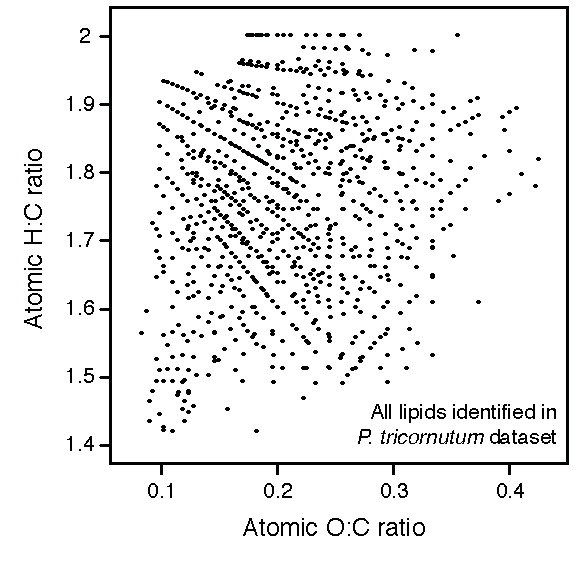
\includegraphics[width=.5\textwidth]{Fig_5-1.pdf}
\captionsetup{font={footnotesize}}
\caption[Basic Van Krevelen plot of the lipid data shown in \autoref{fig:c3n2}a]{Basic Van Krevelen plot of the lipid data shown in \autoref{fig:c3n2}a. Atomic O:C and H:C ratios of the various compounds were determined from elemental formulae.}
\label{fig:c5n1}
\end{SCfigure}

\begin{SCfigure}[1][!t]
\centering
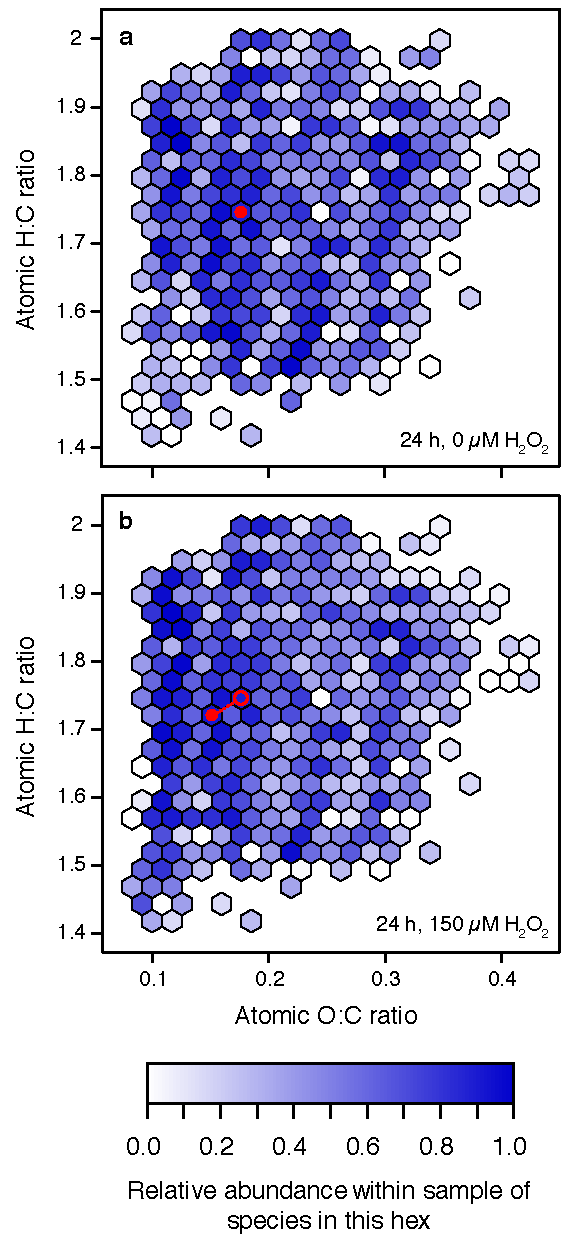
\includegraphics[width=.5\textwidth]{Fig_5-2.pdf}
\captionsetup{font={footnotesize}}
\caption[Hexagonal bin plots in Van Krevelen space of the data shown in \autoref{fig:c3n2}a and \autoref{fig:c5n1}]{Hexagonal bin plot in Van Krevelen space of the data shown in \autoref{fig:c3n2}b and \autoref{fig:c5n1}. Clustering of compounds into hexagonal bins preserves the integrity of the underlying data while reducing complexity to facilitate visual intepretation. (a) and (b) show the compounds identified in \emph{P. tricornutum} after 24 h in, respectively, the 0 $\mu$M H\textsubscript{2}O\textsubscript{2} control and 150 $\mu$M H\textsubscript{2}O\textsubscript{2} treatments. Color density indicates the relative abundance (via log transform and then normalization) of the identified lipid mass within each hex. The filled red symbols show the position in each sample of the bivariate median of the density field; the median position was determined by progressive erosion of hexes in each bin plot. The open red symbol in (b) shows the position of the median in (a), indicating a shift in bulk chemical composition of the \emph{P. tricornutum} lipidome toward the southwest under oxidative stress. This shift reflects the same major trends observed using the hierarchical clustering approach for which results are presented in \autoref{table:adn9} (i.e., apparent acyl elongation and an increase in acyl unsaturation under oxidative stress). Hexagonal binning and identification of the centroid via erosion were peformed using the hexbin package for R (Carr et al., 2015).}
\label{fig:c5n2}
\end{SCfigure}

The utility of the HPLC-MS data screening approach presented in \autoref{chap3} (i.e., \href{https://github.com/vanmooylipidomics/LOBSTAHS}{the LOBSTAHS software}) is limited in its current form by an incomplete understanding of the chemistry that determines the adduct formation hierarchies at the heart of the method. The default adduct ion hierarchies used to identify lipids in \autoref{chap3} and \autoref{chap4}, and \autoref{AppB} (i.e., those given in \autoref{table:adn2}) were determined empirically from repeated observations in the laboratory, and I recommend in \autoref{chap3} that other users of the software make their own empirical observations of formation patterns in all target lipid classes prior to commencing any analysis. However, a mechanistic understanding of the role of chemical structure in determining adduct ion formation patterns in different polar lipids would allow new users to predict hierarchies without direct observations. While relative and absolute adduct ion abundances are often reported in the literature, surprisingly little scientific attention has been given to the underlying chemistry that produces these patterns. This lack of attention is due in no small part to the fact that adduct formation --- and differences in response factors among the different adduct ions of the same precursor --- have been viewed largely as a nuisance to be minimized or a scientific transaction cost associated with HPLC-MS analysis. A few notable exceptions do exist, such as an excellent two-part study by Schug and McNair (Schug and McNair, 2002; 2003), who concluded that differences in adduct ion formation patterns between compounds could be explained by comparison of the acid dissociation constants (p\emph{K\textsubscript{a}}), octanol-water partition coefficients (\emph{K}\textsubscript{\emph{i}ow}) and surface activities of the analytes and the pH, concentration, and type of solvent system. The work by Schug and McNair could provide the basis for a more specific future study of adduct ion formation mechanisms in polar lipids, the results of which could be used to build a predictive tool within LOBSTAHS.

A second limitation of the current approach bears not on its design, but instead on how the hundreds of compounds that can be identified in a single sample are visualized and interpreted. For example, the data presented in \autoref{fig:c3n2} could be reexamined in a Van Krevelen ratio-ratio space, which would allow the user to begin associating changes between treatments with implied chemical mechanisms (\autoref{fig:c5n1}). However, trends can be difficult to discern in a ``simple'' Van Krevelen plot that contains $>$ 10\textsuperscript{3} features, as \autoref{fig:c5n1} illustrates. Alternatively, a hexagonal binning approach could be used to compare the results of different treatments in Van Krevelen space (\autoref{fig:c5n2}); clustering of compounds into hexagonal bins preserves the integrity of the underlying data while reducing complexity to facilitate visual interpretation. In \autoref{fig:c5n2}, the shift in Van Krevelen space of the multivariate median of the data under treatment with 150 $\mu$M H\textsubscript{2}O\textsubscript{2} (red symbol) is indicative of the same major trends that were observed in the \emph{P. tricornutum} experiment using the hierarchical clustering approach for which results are presented in \autoref{table:adn9} (i.e., apparent acyl elongation and an increase in acyl unsaturation under oxidative stress).

\begin{figure}[!th]
\centering
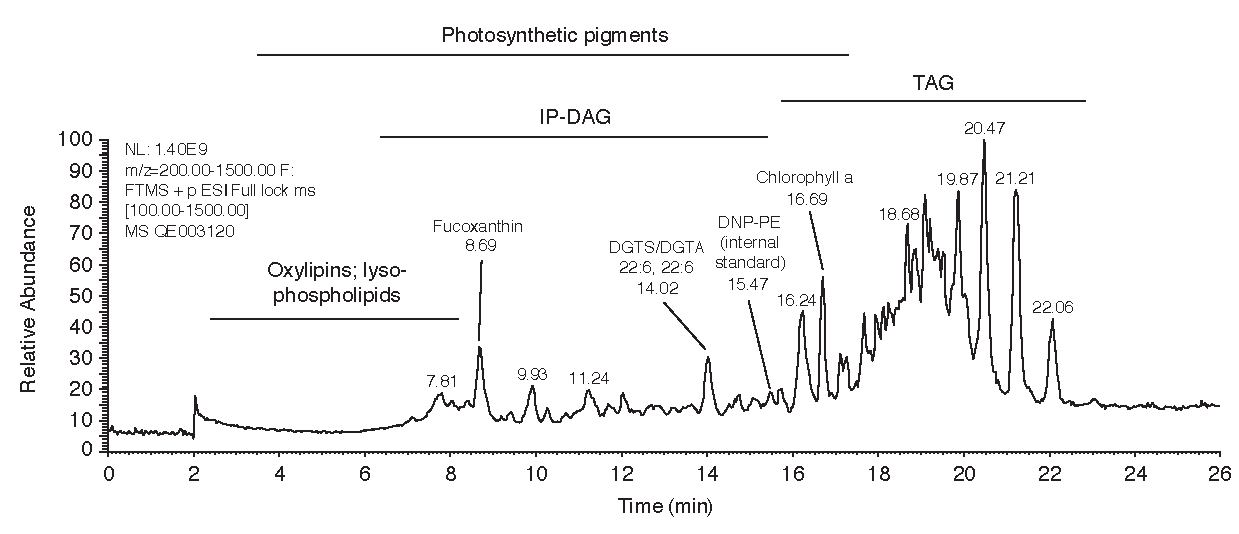
\includegraphics[width=1\textwidth]{Fig_5-3.pdf}
\captionsetup{font={footnotesize}}
\caption[Total ion current chromatogram of a typical marine lipid sample, with annotation of major features]{Total ion current chromatogram (all features, \emph{m/z} 200-1500, positive ionization mode) of a marine lipid sample typical of those described in \autoref{chap4} and \autoref{AppB}. Annotations show major features and retention time ranges for various classes of lipid . This figure shows the same water column sample from Station E, Arthur Habor, West Antarctica, which is presented in the leftmost position in \autoref{fig:c4n10} and \autoref{fig:c4n11}. HRAM-HPLC-ESI-MS analysis and subsequent identification and screening of lipids were performed as described in \autoref{chap4} and \autoref{AppE}.}
\label{fig:c5n3}
\end{figure}

Finally, the results presented in \autoref{chap3}, \autoref{chap4}, and \autoref{AppB} point to a more fundamental limitation of methods such as that described in \autoref{chap3}: The extent to which the mass spectral features in a given set of lipid data can be definitively characterized as individual compounds. One way to evaluate such methods is to examine the fraction of chromatographic peak area that can be identified by the method in a sample of typical complexity. Some performance statistics for the method described in \autoref{chap3} are given in \autoref{table:c3n2}; however, these are based on the number of mass spectral features present in the \emph{P. tricornutum} dataset at various stages of data analysis. Instead, \autoref{table:c5n1} shows the fractions of total chromatographic peak area in a typical environmental lipid sample from \autoref{chap4} (\autoref{fig:c5n3}) that were identified using LOBSTAHS at different levels of certainty. This accounting indicates that LOBSTAHS is capable in its current incarnation of identifying roughly half of the total peak area in the sample recorded for ions between 200 and 1500 \emph{m/z}. That roughly half of the total peak area remains unidentified in a typical sample --- as these results show --- is ample inspiration for improvements to the method. The HPLC-MS features in this unidentified fraction may very well represent additional compounds we would typically consider to be lipids. But it is well worth considering the nonselective nature of a lipid extraction, such as the modified Bligh and Dyer approach used throughout this work: The wide range of \emph{K}\textsubscript{\emph{i}ow} among natural organic compounds (Schwarzenbach et al., 2003) suggests many other hydrophobic molecules we typically do not consider to be lipids will likely almost always be present in the retained organic phase introduced into the mass spectrometer. The development of new methods to characterize this unidentified organic matter --- and improvements to current methods --- will continue to be a key focus of efforts in both biogeochemistry and human biochemistry.

In spite of these limitations, the results in this thesis --- particularly those in \autoref{chap4} and \autoref{AppB} --- demonstrate the potential of high-throughput lipid identification methods to assist biogeochemists and environmental scientists in assessing the impact of various processes and changes in marine ecosystems across a variety of spatial and temporal scales. The results in \autoref{chap4} indicate that changes and differences in ecosystem metalipidome composition can be used to assess shifts in microbial community structure and quantify the effect of various stressors on those communities. Based on this utility, one could make a strong case for the inclusion of such lipid data as a standard time-series measurement within the PAL-LTER and other LTER studies. A full exploitation of these molecules' potential in the context of the PAL-LTER study would require (1) a series of additional experiments to identify compounds diagnostic of various other sources of abiotic and biological stress and (2) characterization of the lipidomes of additional microorganisms important to the ecosystem, particularly those of the cryptomonads which have become an increasingly important component of spring and summer phytoplankton blooms. A commitment to sharing of data and a continuing emphasis on open-source software development will facilitate the production of both improvements and new methods that address these challenges.

\clearpage
\begin{singlespace}
\section*{References}
\addtocounter{section}{1}
{\setlength{\parindent}{0pt}
Alonso-Gonz\'{a}lez, I. J., J. Ar\'{i}stegui, C. Lee, A. Sanchez-Vidal, A. Calafat, J. Fabr\'{e}s, P. Sangr\'{a}, P. Masqu\'{e}, A. Hern\'{a}ndez-Guerra, and V. Ben\'{i}tez-Barrios (2010), Role of slowly settling particles in the ocean carbon cycle, \emph{Geophysical Research Letters}, \emph{37}(13), L13608, doi:\href{http://dx.doi.org/10.1029/2010GL043827}{10.1029/2010GL043827}.

{\setlength{\parskip}{10pt}

Azam, F., D. C. Smith, G. F. Steward, and \AA{}. Hagstr\"{o}m (1994), Bacteria-organic matter coupling and its significance for oceanic carbon cycling, \emph{Microbial Ecology}, \emph{28}(2), 167-179, doi:\href{http://dx.doi.org/10.1007/BF00166806}{10.1007/BF00166806}.

Ducklow, H. W., D. L. Kirchman, H. L. Quinby, C. A. Carlson, and H. G. Dam (1993), Stocks and dynamics of bacterioplankton carbon during the spring bloom in the eastern North Atlantic Ocean, \emph{Deep Sea Research Part II: Topical Studies in Oceanography}, \emph{40}(1-2), 245-263, doi:\href{http://dx.doi.org/10.1016/0967-0645(93)90016-G}{10.1016/0967-0645(93)90016-G}.

Carr, D., N. Lewin-Koh, and M. Maechler (2015), hexbin: Hexagonal Binning Routines, R package version 1.27.1. 

Lancelot, C., and G. Billen (1984), Activity of heterotrophic bacteria and its coupling to primary production during the spring phytoplankton bloom in the Southern Bight of the North Sea, \emph{Limnology \& Oceanography}, \emph{29}(4), 721-730.

Ortega-Retuerta, E., C. G. Fichot, K. R. Arrigo, G. L. Van Dijken, and F. Joux (2014), Response of marine bacterioplankton to a massive under-ice phytoplankton bloom in the Chukchi Sea (Western Arctic Ocean), \emph{Deep Sea Research Part II: Topical Studies in Oceanography}, \emph{105}, 74-84, doi:\href{http://dx.doi.org/10.1016/j.dsr2.2014.03.015}{10.1016/j.dsr2.2014.03.015}.

Riley, J. S., R. Sanders, C. Marsay, F. A. C. Le Moigne, E. P. Achterberg, and A. J. Poulton (2012), The relative contribution of fast and slow sinking particles to ocean carbon export, \emph{Global Biogeochemical Cycles}, \emph{26}(1), GB1026, doi:\href{http://dx.doi.org/10.1029/2011GB004085}{10.1029/2011GB004085}.

Schug, K., and H. M. McNair (2002), Adduct formation in electrospray ionization. Part 1: Common acidic pharmaceuticals, \emph{Journal of Separation Science}, \emph{25}(12), 759-766, doi:\href{http://dx.doi.org/10.1002/1615-9314(20020801)25:12<759::AID-JSSC760>3.0.CO;2-M}{10.100\\2/1615-9314(20020801)25:12<759::AID-JSSC760>3.0.CO;2-M}.

Schug, K., and H. M. McNair (2003), Adduct formation in electrospray ionization mass spectrometry: II. Benzoic acid derivatives, \emph{Journal of Chromatography A}, \emph{985}(1-2), 531-539, doi:\href{http://dx.doi.org/10.1016/S0021-9673(02)01732-6}{10.1016/S0021-9673(02)01732-6}.

Schwarzenbach, R. P., P. M. Gschwend, and D. M. Imboden (2003), Organic liquid-water partitioning, in \emph{Environmental Organic Chemistry}, 2nd ed., pp. 213-244, John Wiley \& Sons Limited, Hoboken, N.J.

Steinberg, D. K., J. S. Cope, S. E. Wilson, and T. Kobari (2008a), A comparison of mesopelagic mesozooplankton community structure in the subtropical and subarctic North Pacific Ocean, \emph{Deep Sea Research Part II: Topical Studies in Oceanography}, \emph{55}(14-15), 1615-1635, doi:\href{http://dx.doi.org/10.1016/J.Dsr2.2008.04.025}{10.1016/J.Dsr2.2008.04.025}.

Steinberg, D. K., B. A. S. Van Mooy, K. O. Buesseler, P. W. Boyd, T. Kobari, and D. M. Karl (2008b), Bacterial vs. zooplankton control of sinking particle flux in the ocean's twilight zone, \emph{Limnology \& Oceanography}, \emph{53}(4), 1327-1338.

Villa-Alfageme, M., F. de Soto, F. A. C. Le Moigne, S. L. C. Giering, R. Sanders, and R. Garc\'{i}a-Tenorio (2014), Observations and modeling of slow sinking particles in the twilight zone, \emph{Global Biogeochemical Cycles}, \emph{28}(11), 1327-1342, doi:\href{http://dx.doi.org/10.1002/2014GB004981}{10.1002/2014GB0\\04981}.}}
\end{singlespace}

\clearpage

\begin{footnotesize}
\begin{singlespace}
\begin{flushleft}
%\renewcommand*{\arraystretch}{1.3}
\begin{longtable}{ Lp{.01\linewidth} Lp{.01\linewidth} Lp{.53\linewidth} Lp{.1\linewidth} Lp{.1\linewidth} Lp{.1\linewidth} }
\captionsetup{font={normalsize}}
\caption[Identification of Chromatographic Peak Area in a Typical Marine Lipid Sample]{Identification of Chromatographic Peak Area in a Typical Marine Lipid Sample}
\label{table:c5n1}
\endfirsthead
\endhead
\toprule
 &  &  & Peak Area $\times10^{9}$ & Fraction Total Peak Area & Fraction Total Putatively Identified Lipids \\
\midrule
%\multicolumn{3}{ p {.55\linewidth} }{Total peak area, 200-1500 m/z, all the way to baseline}  & 462 &  &  \\
\multicolumn{3}{ p {.55\linewidth} }{Total peak area, \emph{m/z} 200-1500} & 153 & 1.00 &  --- \\
\multicolumn{3}{ p {.55\linewidth} }{All lipids putatively identified using LOBSTAHS\textsuperscript{a}}  & 72 & 0.47 & 1.00 \\
 & \multicolumn{2}{ p {.54\linewidth} }{High-confidence compound assignments validated using multiple screening criteria\textsuperscript{b}} &  &  &  \\
 &  & Unoxidized IP-DAG & 7.8 & 0.05 & 0.11 \\
 &  & Photosynthetic pigments & 3.1 & 0.02 & 0.04 \\
 &  & Unoxidized TAG & 55 & 0.36 & 0.77 \\
 &  & DNPPE (internal standard) & 0.4 & $<$ 0.01 & 0.01 \\
 & \multicolumn{2}{ p {.54\linewidth} }{Other\textsuperscript{c}} & 5.4 & 0.04 & 0.07 \\
\bottomrule
\captionsetup{font={footnotesize}}
\caption*{Data in this table are presented for the water column sample shown in the leftmost position in \autoref{fig:c4n10} and \autoref{fig:c4n11}; the corresponding chromatogram is presented in \autoref{fig:c5n3}. HRAM-HPLC-ESI-MS analysis and subsequent identification and screening of lipids were performed as described in \autoref{chap4} and \autoref{AppE}.\\
\textsuperscript{a} See \autoref{chap3} and \autoref{sssec:Chap 4 - Identification and Quantification of Lipids and Oxidized Lipids}. A full list of the LOBSTAHS compound assignments applied to the data can be downloaded from \url{https://github.com/jamesrco/LipidPhotoOxBox/blob/master/data/nice/LOBSTAHS_lipid_identities/PAL1314_LMG1401_particulate_all_LOBSTAHS_IDs_pos.csv} (sample ``QE003120'').\\
\textsuperscript{b} \autoref{sssec:Chap 4 - Identification and Quantification of Lipids and Oxidized Lipids} describes the additional screening criteria we applied. The list of final, high-confidence IP-DAG identified in the sample (\emph{N} = 318; abundances in units of pmol L\textsuperscript{-1}) is contained in \url{https://github.com/jamesrco/LipidPhotoOxBox/blob/master/data/nice/LOBSTAHS_lipid_identities/PAL1314_LMG1401_particulate_IP-DAG_pmol_L.final.csv}.\\
\textsuperscript{c} Includes oxidized lipids, oxylipins, lyso lipids, and low-confidence compound assignments of unoxidized species.\\
}
\end{longtable}
\end{flushleft}
\end{singlespace}
\end{footnotesize}
\appendix
\include{AppA}
\include{AppB}
\include{AppC}
\include{AppD}
\include{AppE}
\include{AppF}

\end{document}

